% Options for packages loaded elsewhere
% Options for packages loaded elsewhere
\PassOptionsToPackage{unicode}{hyperref}
\PassOptionsToPackage{hyphens}{url}
%
\documentclass[
  letterpaper,
]{tex/uofsthesis-cs}
\usepackage{xcolor}
\usepackage{amsmath,amssymb}
\setcounter{secnumdepth}{5}
\usepackage{iftex}
\ifPDFTeX
  \usepackage[T1]{fontenc}
  \usepackage[utf8]{inputenc}
  \usepackage{textcomp} % provide euro and other symbols
\else % if luatex or xetex
  \usepackage{unicode-math} % this also loads fontspec
  \defaultfontfeatures{Scale=MatchLowercase}
  \defaultfontfeatures[\rmfamily]{Ligatures=TeX,Scale=1}
\fi
\usepackage{lmodern}
\ifPDFTeX\else
  % xetex/luatex font selection
\fi
% Use upquote if available, for straight quotes in verbatim environments
\IfFileExists{upquote.sty}{\usepackage{upquote}}{}
\IfFileExists{microtype.sty}{% use microtype if available
  \usepackage[]{microtype}
  \UseMicrotypeSet[protrusion]{basicmath} % disable protrusion for tt fonts
}{}
\makeatletter
\@ifundefined{KOMAClassName}{% if non-KOMA class
  \IfFileExists{parskip.sty}{%
    \usepackage{parskip}
  }{% else
    \setlength{\parindent}{0pt}
    \setlength{\parskip}{6pt plus 2pt minus 1pt}}
}{% if KOMA class
  \KOMAoptions{parskip=half}}
\makeatother
% Make \paragraph and \subparagraph free-standing
\makeatletter
\ifx\paragraph\undefined\else
  \let\oldparagraph\paragraph
  \renewcommand{\paragraph}{
    \@ifstar
      \xxxParagraphStar
      \xxxParagraphNoStar
  }
  \newcommand{\xxxParagraphStar}[1]{\oldparagraph*{#1}\mbox{}}
  \newcommand{\xxxParagraphNoStar}[1]{\oldparagraph{#1}\mbox{}}
\fi
\ifx\subparagraph\undefined\else
  \let\oldsubparagraph\subparagraph
  \renewcommand{\subparagraph}{
    \@ifstar
      \xxxSubParagraphStar
      \xxxSubParagraphNoStar
  }
  \newcommand{\xxxSubParagraphStar}[1]{\oldsubparagraph*{#1}\mbox{}}
  \newcommand{\xxxSubParagraphNoStar}[1]{\oldsubparagraph{#1}\mbox{}}
\fi
\makeatother


\usepackage{longtable,booktabs,array}
\usepackage{calc} % for calculating minipage widths
% Correct order of tables after \paragraph or \subparagraph
\usepackage{etoolbox}
\makeatletter
\patchcmd\longtable{\par}{\if@noskipsec\mbox{}\fi\par}{}{}
\makeatother
% Allow footnotes in longtable head/foot
\IfFileExists{footnotehyper.sty}{\usepackage{footnotehyper}}{\usepackage{footnote}}
\makesavenoteenv{longtable}
\usepackage{graphicx}
\makeatletter
\newsavebox\pandoc@box
\newcommand*\pandocbounded[1]{% scales image to fit in text height/width
  \sbox\pandoc@box{#1}%
  \Gscale@div\@tempa{\textheight}{\dimexpr\ht\pandoc@box+\dp\pandoc@box\relax}%
  \Gscale@div\@tempb{\linewidth}{\wd\pandoc@box}%
  \ifdim\@tempb\p@<\@tempa\p@\let\@tempa\@tempb\fi% select the smaller of both
  \ifdim\@tempa\p@<\p@\scalebox{\@tempa}{\usebox\pandoc@box}%
  \else\usebox{\pandoc@box}%
  \fi%
}
% Set default figure placement to htbp
\def\fps@figure{htbp}
\makeatother


% definitions for citeproc citations
\NewDocumentCommand\citeproctext{}{}
\NewDocumentCommand\citeproc{mm}{%
  \begingroup\def\citeproctext{#2}\cite{#1}\endgroup}
\makeatletter
 % allow citations to break across lines
 \let\@cite@ofmt\@firstofone
 % avoid brackets around text for \cite:
 \def\@biblabel#1{}
 \def\@cite#1#2{{#1\if@tempswa , #2\fi}}
\makeatother
\newlength{\cslhangindent}
\setlength{\cslhangindent}{1.5em}
\newlength{\csllabelwidth}
\setlength{\csllabelwidth}{3em}
\newenvironment{CSLReferences}[2] % #1 hanging-indent, #2 entry-spacing
 {\begin{list}{}{%
  \setlength{\itemindent}{0pt}
  \setlength{\leftmargin}{0pt}
  \setlength{\parsep}{0pt}
  % turn on hanging indent if param 1 is 1
  \ifodd #1
   \setlength{\leftmargin}{\cslhangindent}
   \setlength{\itemindent}{-1\cslhangindent}
  \fi
  % set entry spacing
  \setlength{\itemsep}{#2\baselineskip}}}
 {\end{list}}
\usepackage{calc}
\newcommand{\CSLBlock}[1]{\hfill\break\parbox[t]{\linewidth}{\strut\ignorespaces#1\strut}}
\newcommand{\CSLLeftMargin}[1]{\parbox[t]{\csllabelwidth}{\strut#1\strut}}
\newcommand{\CSLRightInline}[1]{\parbox[t]{\linewidth - \csllabelwidth}{\strut#1\strut}}
\newcommand{\CSLIndent}[1]{\hspace{\cslhangindent}#1}



\setlength{\emergencystretch}{3em} % prevent overfull lines

\providecommand{\tightlist}{%
  \setlength{\itemsep}{0pt}\setlength{\parskip}{0pt}}



 


\usepackage{setspace}

\degree{\PhD}
\department{Geography and Planning\\
  (Centre for Hydrology)}
\defencedate{November 2025}
\ptuaddress{Head of the Department of Geography and Planning\\
  117 Science Place\\
  University of Saskatchewan\\
  Saskatoon, Saskatchewan, S7N 5C8\\
  Canada}

% abstract.tex
\thesisabstract{%
Partitioning of snow in needleleaf canopies by interception and ablation processes regulates the quantity, timing, and phase of precipitation that reaches the ground in cold region forests. Sparse observations have limited understanding of these processes and hindered their representation in hydrological and land-surface models. Consequently, simulations of subcanopy snow accumulation have shown variable accuracy across different climates and canopy structures, and diagnosing the causative processes that partition snowfall in needleleaf forests remains difficult. This study aims to better understand partitioning of snowfall in forest canopies to better predict snow accumulation in forested environments and subsequent water resources. To achieve this goal a comprehensive review of the literature was conducted, in-situ observations of forest-snow processes and subcanopy snow accumulation were collected to evaluate the theories underlying existing parameterisations, derive new relationships, and validate a newly proposed model. 

The results from the literature review demonstrated that existing parameterisations for snow interception and canopy snow ablation have incomplete and potentially duplicated process representation. For example, existing studies show that existing snow interception parameterisations may overemphasize the influence of canopy snow load on throughfall. This association has been attributed to either reduced canopy coverage due to branch bending [@Schmidt1990; @Schmidt1991] and/or increased rates of unloading. @Staines2023 showed using novel aerial lidar based observations of canopy density and throughfall found limited influence of snow load on canopy coverage due to branch bending. Therefore, if the relationship of initial interception with snow load is not resulting from canopy density changes, perhaps it may be better represented using the unloading parameterisation alone to avoid double counting this process. Moreover, the methodologies used to parameterise non-melt induced canopy snow unloading routines rely on indirect measurements and should be assessed using more direct measurements. While many canopy snow ablation processes occur simultaneously using a hybrid modelled-observed processes to help isolate individual canopy snow processes has not been utilised to help understand canopy snow processes. Existing studies on snowfall partitioning by forest canopies have largely focused on forests with high density canopies and either cold continental or warm maritime climates. While differing process representations have resulted from these distinct climates, this literature review suggests that the methodological differences used to measure snow interception and ablation processes likely also contributed to the differing theories. 

New observations of initial snow interception, collected when ablation processes were minimal, showed that canopy density is the primary factor influencing subcanopy snow throughfall. Contrary to existing theories, no relationships were found with canopy snow load or air temperature. Canopy density was best represented by a snow-leaf contact area metric, which accounts for increasing contact area with more horizontal snowfall trajectories. This metric was highly sensitivity to wind speed in sparse canopies, increasing by up to an order of magnitude with a 1 m s$^{-1}$ wind speed. A new parameterisation was developed that calculates throughfall as a function of snowfall and snow-leaf contact area based on these observations. This approach is consistent with some rainfall interception studies, which also separate canopy loading and ablation processes, and calculate interception as a function of canopy cover.

Observations showed that canopy snow unloading was strongly associated with snow load, wind shear stress, and canopy snowmelt. A new canopy snow ablation model was developed based on these associations and their impact on the canopy snow energy and mass balance. The model improved simulation of canopy snow load relative to previous approaches, especially for melt- and wind-dominated ablation events. The improved performance in representing canopy snow load compared to existing models results from including energy balance-based melt and dry snow unloading relationships with snow load and wind shear stress. The inclusion of both melt and dry snow unloading processes in the new model also led to more accurate partitioning of snowfall to the atmosphere versus the ground compared to existing approaches across a wide range of meteorologies.

Validation of the revised canopy snow mass and energy balance was conducted at four needleleaf forests characterised by differing tree species, canopy structure, and meteorological conditions. The new physically based approach reduced error in simulating subcanopy snow water equivalent (SWE) compared to an existing model. Improved process representation also enabled clearer process diagnosis on the influence of vegetation on snow accumulation. At two cold, low-snowfall sites, roughly half of annual snowfall was lost to the atmosphere via sublimation of intercepted snow. A cold wind-exposed site with higher annual snowfall had increased unloading rates and reduced atmospheric losses. In contrast, at a temperate-maritime site, nearly half of annual snowfall melted within the canopy, and combined with melt-induced unloading led to the lowest fraction of snowfall lost through canopy snow sublimation.

This research identified key limitations in existing models using in-situ process-level observations of snow interception and ablation. New parameterisations of the canopy snow mass and energy balance are introduced to more explicitly represent the processes that govern snowfall partitioning in needleleaf canopies. This new approach led to more accurate simulations of canopy snow load and subcanopy SWE across a broad range of meteorologies and forest types and also improved process diagnosis, though further validation is required across a diverse range of sites.
}

% acknowledgements.tex
\thesisacknowledgements{%
I am incredibly thankful for random text Fuerint certius dormire duratio expirat mea has agendis. Sequeretur et praecipuus recensenda du gi pensitatis ei intelligam. Est externarum sit scripturas praemissae. Nulla demus has rebus timet sui mecum certe. Facultate affirmare is ac priusquam tribuebam potentiam et ex continent. Unam pati suae vice hos luce addi dem. Meos ipsa atra vi unam in tale. Reges istam mundo spero ad at ha nolle.
}

% dedication.tex
\thesisdedication{%
"Human nature is like water. It takes the shape of its container.”
}


% Switch for main body, prevents stretching of last page on chapters and leaves portion of page blank
\raggedbottom
\usepackage{booktabs}
\usepackage{caption}
\usepackage{longtable}
\usepackage{colortbl}
\usepackage{array}
\usepackage{anyfontsize}
\usepackage{multirow}
\makeatletter
\@ifpackageloaded{bookmark}{}{\usepackage{bookmark}}
\makeatother
\makeatletter
\@ifpackageloaded{caption}{}{\usepackage{caption}}
\AtBeginDocument{%
\ifdefined\contentsname
  \renewcommand*\contentsname{Table of contents}
\else
  \newcommand\contentsname{Table of contents}
\fi
\ifdefined\listfigurename
  \renewcommand*\listfigurename{List of Figures}
\else
  \newcommand\listfigurename{List of Figures}
\fi
\ifdefined\listtablename
  \renewcommand*\listtablename{List of Tables}
\else
  \newcommand\listtablename{List of Tables}
\fi
\ifdefined\figurename
  \renewcommand*\figurename{Figure}
\else
  \newcommand\figurename{Figure}
\fi
\ifdefined\tablename
  \renewcommand*\tablename{Table}
\else
  \newcommand\tablename{Table}
\fi
}
\@ifpackageloaded{float}{}{\usepackage{float}}
\floatstyle{ruled}
\@ifundefined{c@chapter}{\newfloat{codelisting}{h}{lop}}{\newfloat{codelisting}{h}{lop}[chapter]}
\floatname{codelisting}{Listing}
\newcommand*\listoflistings{\listof{codelisting}{List of Listings}}
\makeatother
\makeatletter
\makeatother
\makeatletter
\@ifpackageloaded{caption}{}{\usepackage{caption}}
\@ifpackageloaded{subcaption}{}{\usepackage{subcaption}}
\makeatother
\usepackage{bookmark}
\IfFileExists{xurl.sty}{\usepackage{xurl}}{} % add URL line breaks if available
\urlstyle{same}
\hypersetup{
  pdftitle={Advancing Snow Accumulation Models in Needleleaf Forests},
  pdfauthor={Alex C. Cebulski},
  hidelinks,
  pdfcreator={LaTeX via pandoc}}


% This just links the title/author defined in yaml over the the frontmatter section in the cls
\title{Advancing Snow Accumulation Models in Needleleaf Forests}
\author{Alex C. Cebulski}

\begin{document}
%%%%% CHOOSE YOUR LINE SPACING HERE
% This is the official option.  Use it for your submission copy and library copy:
% \setlength{\textbaselineskip}{22pt plus2pt}
% This is closer spacing (about 1.5-spaced) that you might prefer for your personal copies:
%\setlength{\textbaselineskip}{18pt plus2pt minus1pt}

% You can set the spacing here for the roman-numbered pages (acknowledgements, table of contents, etc.)
% \setlength{\frontmatterbaselineskip}{17pt plus1pt minus1pt}

% Leave this line alone; it gets things started for the real document.
% \setlength{\baselineskip}{\textbaselineskip}

% The level that gets a number:
% \setcounter{secnumdepth}{2}
% % The level that shows up in the ToC:
% \setcounter{tocdepth}{2}
%
% \newpage
% \thispagestyle{empty}
% \null
% \newpage
% JEM: Pages are roman numbered from here, though page numbers are invisible until ToC.  This is in
% keeping with most typesetting conventions.
% \pagenumbering{roman}

% \begin{romanpages}

% Title page is created here
\maketitle

\frontmatter

%%%%% DEDICATION -- If you'd like one, un-comment the following.

% \begin{dedication}
%     \input{frontmatter/01-dedication.txt}
% \end{dedication}

%%%%% Declaration -- Nothing to do here except comment out if you don't want it.

% \begin{declaration}
% \addcontentsline{toc}{chapter}{Declaration}
% 	\input{frontmatter/02-declaration.txt}
%     \vspace{0.5em}
%     \begin{flushright}
%       \includegraphics[width=4 cm]{frontmatter/figs/signature.jpg}
%     \end{flushright}
%     \vspace{0.5em}
%     \begin{flushright}
%       {\large \textit{Alex C. Cebulski}}
%     \end{flushright}
%     \vspace{0.5em}
%     \noindent Word Count: 
%     \vfill
%     \noindent This thesis was conducted under the supervision of .
%     \vspace{2cm}
% \end{declaration}

%%%%% ABSTRACT -- Nothing to do here except comment out if you don't want it.

% \begin{abstract}
% \addcontentsline{toc}{chapter}{Abstract}
% 	\input{frontmatter/02-abstract.txt}
% \end{abstract}

%%%%% ACKNOWLEDGEMENTS -- Nothing to do here except comment out if you don't want it.

% \begin{acknowledgements}
% \addcontentsline{toc}{chapter}{Acknowledgements}
%  	\input{frontmatter/03-acknowledgements.txt}
% \end{acknowledgements}

% This aligns the bottom of the text of each page.  It generally makes things look better.
% \flushbottom

\bookmarksetup{startatroot}

\chapter{Introduction}\label{introduction}

Melt of the seasonal snowpack directly supports over two billion people
worldwide---crucial for downstream ecosystems, energy production, and
agricultural irrigation (Immerzeel et al., 2020; Viviroli et al., 2020).
The high albedo and energy required to melt snow also provides a
large-scale cooling effect for our planet by reflecting most of the
incoming solar radiation and dissipating energy during spring melt
(Henderson et al., 2018; Leach \& Moore, 2014). Snowfall in forested
areas occurs over 50\% of the northern hemisphere (Kim et al., 2017),
and over 20\% of the global landmass (Deschamps-Berger et al., 2025).
Intercepted snow in the canopy is subjected to higher rates of
sublimation and melt compared to the subcanopy snowpack due to greater
surface area, turbulent energy exchange, and solar exposure (Floyd,
2012; Pomeroy et al., 1998b; Storck et al., 2002). In cold-dry
continental climates, researchers estimate that 25 to 45\% of annual
snowfall may be lost to the sublimation of intercepted snow from the
canopy (Essery et al., 2003; Sanmiguel-Vallelado et al., 2017). In
warm-humid maritime climates the majority of snowfall melts in the
canopy (Floyd, 2012; Storck et al., 2002), limiting atmospheric losses
from sublimation, and contributes to changes in the phase and timing of
precipitation reaching the subcanopy. The strong hydrological influence
of forest canopies leads to high variability of snowpack accumulation in
forested basins. Observations of this variability is not well
represented due to a sparse and unrepresentative network of in situ
observations, which are mostly located in clearings (Vionnet et al.,
2021). Moreover, observing snow accumulation under forest canopies at
large extents remains uncertain with current remote sensing technologies
(Rittger et al., 2020). Thus, there is a need for reliable models of
snow redistribution by forest to estimate snow accumulation (Clark et
al., 2015a; Pomeroy et al., 2022) and to diagnose the impact of changing
climate and vegetation cover on snowpack accumulation (Immerzeel et al.,
2020; López-Moreno et al., 2014; Viviroli et al., 2020).

Limited observations of forest-snow processes including throughfall,
unloading, sublimation, drip, and melt of canopy snow have limited
process understanding and led to uncertainties in representing these
processes in hydrological models (Lundquist et al., 2021). Existing snow
interception parameterisations have been developed for both warm
maritime (Andreadis et al., 2009; Storck et al., 2002) and cold
continental (Ellis et al., 2010; Hedstrom \& Pomeroy, 1998; Roesch et
al., 2001) climates characterized by dense forest canopy. The strong
dependence of snowfall partitioning by vegetation on meteorology and
canopy density has challenged earlier parameterisations that were
developed and tested in distinct climates in dense forest canopies. As a
result these parameterisations often need to be calibrated when applied
to new sites to better represent canopy snow interception (e.g.,
Lumbrazo et al., 2022). Although accurate performance in simulating
subcanopy snow water equivalent (SWE) has been achieved across different
climates in some studies (Essery \& Pomeroy, 2004; Gelfan et al., 2004),
other snow model comparisons (Krinner et al., 2018; Rutter et al., 2009)
have shown limited performance. The omission or simplified
representation of processes and reliance on empirically derived
coefficients likely contribute to model uncertainty when applied in
climates and forests other than where they were developed (Krinner et
al., 2018; Lumbrazo et al., 2022; Lundquist et al., 2021; Roth \& Nolin,
2019; Rutter et al., 2009).

In hydrological models, the partitioning of snowfall in forest canopies
is typically handled by first calculating the fraction of snowfall that
is intercepted in the canopy (initial interception) and also
parameterisations for ablation processes including unloading, melt/drip,
and sublimation (Clark et al., 2015a; Pomeroy et al., 2022). Lundquist
et al. (2021) and Staines \& Pomeroy (2023) show that parameterisations
developed by Hedstrom \& Pomeroy (1998) and Storck et al. (2002)
typically used in hydrological and land surface models (Clark et al.,
2015a; Pomeroy et al., 2022; Verseghy, 2017) may overemphasize the role
of increasing canopy snow load increasing throughfall of snow in the
initial interception process. However, the snow loads observed by
Staines \& Pomeroy (2023) were relatively small, and thus their
observations should be confirmed using additional observations over
larger snowfall events and variable canopy densities and also over
longer timescales. Several studies emphasize the importance of
representing both dry/cold- and melt-induced unloading of snow in the
canopy (Ellis et al., 2010; Essery \& Pomeroy, 2004; Gelfan et al.,
2004; Roesch et al., 2001). These processes are supported through
physical mechanisms such as loss of structural integrity, particle bond
weakening, and lubrication of intercepted snow during the melt process
(Floyd, 2012; Storck et al., 2002). Sublimation promotes unloading via
structural degradation and bond weakening of intercepted snow
(MacDonald, 2010). Wind drag promotes unloading through shear stress
applied to intercepted snow, wind erosion through direct entrainment in
the atmosphere of intercepted snow, and branch movement (Bartlett \&
Verseghy, 2015; Lumbrazo et al., 2022; Roesch et al., 2001). Increasing
air temperature promotes unloading by increasing the elasticity of
branches and its association with melt and/or sublimation (Schmidt \&
Gluns, 1991; Schmidt \& Pomeroy, 1990). While direct measurements of
canopy snow unloading associated with melt were provided using detailed
process-level lysimetry by Storck et al. (2002) dry-snow unloading
parameterisation have been developed using indirect measurements from
above canopy albedo (Bartlett \& Verseghy, 2015; Roesch et al., 2001).
Therefore, validation of the theories underlying dry-snow unloading
parameterisations would benefit from additional direct observations of
canopy snow unloading. Moreover, the canopy snowmelt induced unloading
association proposed by Storck et al. (2002) was based on a single event
and thus should be validated using additional observations. Additional
processes currently not encoded in snow interception models include wind
redistribution of snow, rain on intercepted snow, hoarfrost, rime ice
and the cohesion and adhesion of snow in the canopy which will also be
investigated.

Future climate change is expected to change the dominant hydrological
processes in mountain forests largely as a result of the dependence of
many snow processes on temperature (Dettinger, 2014; Fang \& Pomeroy,
2020; He et al., 2021; Viviroli et al., 2011). A report by Environment
and Climate Change Canada (Bush \& Lemmen, 2019), suggest an increase in
air temperature of 2 °C from the 1986-2005 reference period by 2050 for
the low emission scenario and 6 °C for the high emission scenario by the
late 21\textsuperscript{st} century. Bush \& Lemmen (2019) project an
increase in annual mean precipitation over all of Canada during the
second half of the 21\textsuperscript{st} century, with a larger
increase in northern Canada. As the climate warms, regions such as
continental climates in Canada may shift from a dry-snow unloading and
sublimation dominated regime to more influences from canopy snowmelt and
drip processes. Thus, additional investigations on both melt- and
dry-snow unloading are warranted to better understand both processes
that are expected to become more prevalent in Canada with climate
change.

In addition to shifting snow processes as a result of climate change,
vegetation cover has already started experiencing changes resulting from
drought (Dai, 2013), disease (Ruess et al., 2021), insects (Kurz et al.,
2008), fire (Kasischke et al., 2010; Kasischke \& Turetsky, 2006),
changing land use (López-Moreno et al., 2014), and changing species
(Gottfried et al., 2012). These changes in temperature, precipitation,
along with the changing forest species, structure, and density are
expected to have strong impacts on snowpack accumulation worldwide.
However, to better understand these impacts, greater confidence in the
application of forest-snow process parameterisations is needed. Since
snow interception and ablation parameterisation were developed in
distinct cold or warm climates with dense canopy structure there is a
need to ensure these parameterisations are transferable across diverse
climate and forest canopies.

To assess the performance of existing parameterisations, a modular and
flexible model platform will be used to simulate the individual mass and
energy balance fluxes and states of the canopy and snowpack. The
advantage of modular and flexible model platforms is that it is possible
to adjust process parameterisations while holding the remaining model
parameters and mass and energy conservation equations constant (Clark et
al., 2015a; Pomeroy et al., 2022). The Cold Regions Hydrological Model
platform (CRHM, Pomeroy et al., 2022) will be used in this study as its
mass and energy balance parameterisations have been successfully used in
previous studies (Ellis et al., 2010; Pomeroy et al., 2012; Rasouli et
al., 2019b; Sanmiguel-Vallelado et al., 2022a) to assess forest-snow
interactions in Spain, USA, and Canada. Since CRHM is a process-based
model agnostic platform, individual state and flux variables including
subcanopy snow accumulation, snow interception, sublimation, unloading,
drip, and wind redistribution can be evaluated using differing
parameterisations. To evaluate existing parameterisations of snow
interception (Andreadis et al., 2009; Hedstrom \& Pomeroy, 1998; Storck
et al., 2002), and ablation of canopy snow by unloading (Andreadis et
al., 2009; Ellis et al., 2010; Roesch et al., 2001), drip (Andreadis et
al., 2009; Ellis et al., 2010; Storck et al., 2002) and sublimation
(Pomeroy et al., 1998b) CRHM will be run at four mountain forest
research basins in western and northern Canada and compared to in-situ
observations of subcanopy SWE. Modifications to the existing
parameterisations to better represent snow interception processes will
be validated on the associated change in error in simulated and observed
forest snow accumulation.

\section{Research Objectives}\label{research-objectives}

The overarching goal of this thesis is to better understand the dominant
processes that govern snow accumulation in forested environments and to
determine how these processes can be accurately represented in
hydrological models. To achieve this goal, two specific research
objectives were formulated each with underlying research question(s):

\subsection{Objective 1: Evaluate the suitability of existing snow
interception and ablation parameterisations for application in
needleleaf forests with differing canopy structure and
meteorology.}\label{objective-1-evaluate-the-suitability-of-existing-snow-interception-and-ablation-parameterisations-for-application-in-needleleaf-forests-with-differing-canopy-structure-and-meteorology.}

\begin{enumerate}
\def\labelenumi{\arabic{enumi}.}
\item
  What are the theoretical underpinnings and assumptions behind existing
  snow interception and ablation parameterisations?
\item
  Are the theories and assumptions of existing snow interception
  parameterisations supported by field measurements collected across
  diverse canopy structures and meteorological conditions?
\item
  Are the theories and assumptions of existing canopy snow ablation
  parameterisations supported by field measurements collected across
  varying meteorological conditions?
\end{enumerate}

\subsection{Objective 2: Determine how new snow interception and
ablation parameterisations could enhance the representation of processes
important for subcanopy snow
accumulation.}\label{objective-2-determine-how-new-snow-interception-and-ablation-parameterisations-could-enhance-the-representation-of-processes-important-for-subcanopy-snow-accumulation.}

\begin{enumerate}
\def\labelenumi{\arabic{enumi}.}
\setcounter{enumi}{3}
\tightlist
\item
  How can the use of novel snow interception parameterisations enhance
  simulations of snow accumulation in forests with differing tree
  species, canopy structures, and meteorological conditions?
\end{enumerate}

\section{Organization of Chapters}\label{organization-of-chapters}

Following the Introduction of the thesis (Chapter 1), four manuscripts
are presented as thesis chapters designed for submission to
peer-reviewed journals and correspond to the aforementioned four
research questions. Chapter 2 addresses Research Question 1 by providing
a comprehensive review of the literature on snow interception and
ablation parameterisations. This review identified the theories and
assumptions underlying existing parameterisations and highlights the
primary research gaps that this thesis seeks to address. The outcomes of
Chapter 2 provide the foundation for evaluating parameterisations using
field observations in the subsequent chapters.

Chapter 3 addresses Research Question 2 by presenting an evaluation of
snow interception relationships based on novel observations of
throughfall and canopy density. The results demonstrate theories
underlying existing snow interception parameterisations are not
supported and show improved representation of the initial interception
process with a new parameterisation across diverse meteorology, snow
loads, and canopy densities.

Chapter 4 addresses Research Question 3 through an evaluation of
theories regarding canopy snow ablation processes using a hybrid
diagnostic mass balance approach which combined both direct observations
of individual canopy snow ablation processes with simulations---where
some process observations were not available (i.e., canopy snow
sublimation). The results reveal that canopy snow load, wind shear
stress, and snowmelt were most strongly associated with unloading and
differed from existing theories. These findings highlight the need for
revised parameterisations to accurately represent canopy snow ablation.
Collectively, Chapters 2 through 4 demonstrate the successful completion
of Objective 1.

Chapter 5 addresses Objective 2 (and Research Question 4) and describes
the development of a new canopy snow model that incorporates the
relationships identified in Chapters 3 and 4. The model is implemented
in the Cold Regions Hydrological Modelling Platform across four research
sites in western and northern Canada. Results demonstrate improved
simulations of subcanopy SWE, especially under warm-humid climates
dominated by canopy snow melt, validating the new parameterisations.

The thesis concludes with Chapter 6 which provides a synthesis of the
results and conclusions from the previous chapters.

\pagebreak

\bookmarksetup{startatroot}

\chapter{The Theoretical Underpinnings of Existing Snow Interception and
Ablation
parameterisations}\label{the-theoretical-underpinnings-of-existing-snow-interception-and-ablation-parameterisations}

Manuscript Status: The contents of this chapter have been compiled from
a advanced review article published in the journal \emph{WIREs Water}.

Citation: Cebulski, A. C., \& Pomeroy, J. W. (2025). Theoretical
Underpinnings of Snow Interception and Canopy Snow Ablation
Parameterisations. \emph{WIREs Water}, 12, e70010.
https://doi.org/10.1002/wat2.70010

Role in thesis: This paper is an advanced review article and corresponds
to objective 1, research question 1.1 of the thesis. This advanced
review will provide the context necessary for interpreting whether the
theories and assumptions of existing parameterisations are true for the
field observations collected in this study in the second part of
objective 1.

Author Contribution:

A. Cebulski: Conceptualization (lead), investigation (equal), software
(lead), visualization (lead), writing -- original draft (lead), writing
review and editing (equal) J. Pomeroy: Conceptualization (supporting),
funding acquisition (lead), investigation (equal), project
administration (lead), resources (lead), supervision (lead), writing
review and editing (equal).

\section{Abstract}\label{abstract}

In needleleaf forests, up to half of annual snowfall may be returned to
the atmosphere through sublimation of snow intercepted in the canopy.
However, limited and sparse observations of snow interception and
ablation processes have hindered the development of fundamental theories
underpinning current estimates of snow accumulation in forests. Existing
parameterisations for snow interception and ablation have been developed
in locations with distinctive climate, tree species and forest
structures, resulting in inconsistent and non-comprehensive process
representations. This variability limits the transferability of these
parameterisations across diverse landscapes and climates. Moreover,
difficulties in isolating individual processes in field-based
measurements has led to parameterisations that inadvertently coupled
multiple processes, adding to uncertainty. Many studies have also
simplified original parameterisations and do not include recent advances
from observational studies. This review article aims to elucidate the
theoretical foundations and assumptions underlying the current snow
interception and ablation parameterisations to provide a better
understanding of uncertainties in existing methods and identify
priorities for future field-based observational studies. The methods
behind snow interception and ablation studies are also reviewed to
provide necessary context for examining current parameterisations.
Specific gaps in the literature include determining the canopy snow
storage capacity, challenges in distinguishing snow throughfall
measurements from canopy snow ablation, partitioning unloading rates and
canopy snowmelt drainage, the assumption of vertical falling hydrometeor
trajectories, the absence of wind resuspension parameterisations, and
the limited testing of parameterisations in varied forests and climates.

\section{Introduction}\label{introduction-1}

The melt of seasonal snowpacks is an important source of streamflow
around the world, crucial for downstream ecosystems, energy production,
drinking water supply and agricultural irrigation that directly support
over 2 billion people (Viviroli et al., 2007, 2020). Despite this
importance, there is uncertainty in estimates of snow accumulation due
to redistribution of snow by wind and forest canopy (Ellis et al., 2010;
Krinner et al., 2018; Rutter et al., 2009). In the Northern Hemisphere,
over 50\% of snowmelt-dominated basins are covered by needleleaf forest
(Kim et al., 2017). This extensive canopy coverage reduces the amount of
snow that is available for streamflow through interception of snowfall
and subsequent canopy snow sublimation (Ellis et al., 2010; Essery et
al., 2003; Hedstrom \& Pomeroy, 1998). Intercepted snow in the canopy is
subjected to higher rates of sublimation and melt compared to subcanopy
snow due to greater surface area, warmer temperatures, turbulent energy
exchange and solar exposure (Lundberg \& Halldin, 1994; Pomeroy et al.,
1998b). Across the Northern Hemisphere, researchers have estimated that
25--45\% of annual snowfall may be lost to the sublimation of
intercepted snow from the canopy (Essery et al., 2003). However, the
magnitude of sublimation losses depends on the amount of snowfall that
is intercepted in the canopy and the competing ablation processes
including unloading, melt, drip, and resuspension of snow that control
the duration that snow resides in the canopy. These processes contribute
to spatial and temporal variability in the accumulation of snowpacks
both between and within forested and non-forested landscapes (Krinner et
al., 2018; Rutter et al., 2009). This snowpack variability is not well
represented due to a sparse and unrepresentative network of in-situ
observations, which are mostly located in forest clearings (e.g.,
Canada, Vionnet et al., 2021). Moreover, while high spatial resolution
snow depth measurements from aerial lidar are useful for canopy-snow
process investigations at the plot scale (e.g., Staines \& Pomeroy,
2023), observing snow accumulation under forest canopies at large
extents remains uncertain with current remote sensing technologies
(Rittger et al., 2020; Stillinger et al., 2023). Therefore, there is a
need for robust models of snow redistribution by vegetation to estimate
snow accumulation in forests and generate predictions of how water
resources will change with future climates (Clark et al., 2015a; Pomeroy
et al., 2007; Rutter et al., 2009). Such models require a comprehensive
understanding of snow redistribution processes.

Existing theories of snow interception and ablation have primarily been
developed for dense forest canopies in either warm maritime (Andreadis
et al., 2009; Katsushima et al., 2023; Storck et al., 2002) or cold
continental (Ellis et al., 2010; Hedstrom \& Pomeroy, 1998; Roesch et
al., 2001) climates. These isolated observations have resulted in
distinctive theories of the key snow interception and ablation
processes. Whilst parameterisations founded on these theories can yield
accurate simulations of the timing and magnitude of forest snow
accumulation when applied in similar climates to where they were
developed (Lundquist et al., 2021; Rasouli et al., 2019a; Roth \& Nolin,
2019) or when combined into a hybrid parameterisation and assessed at
global and regional scales in a wide range of climates (Essery et al.,
2003; Gelfan et al., 2004), large discrepancies in simulated subcanopy
snow accumulation have been demonstrated in inter-model comparisons by
(Krinner et al., 2018) and (Rutter et al., 2009). Some of the
uncertainty in subcanopy snowpack simulations observed by (Krinner et
al., 2018) and (Rutter et al., 2009) was attributed to differing snow
interception and ablation process representation, in addition to model
platform differences (Clark \& Kavetski, 2010). One example of differing
process behaviour is the increase in canopy snow storage capacity with
warmer temperatures shown by (Storck et al., 2002) and an opposing
relationship suggested by (Hedstrom \& Pomeroy, 1998). The difficulty in
isolating individual processes such as throughfall, unloading, and drip
in field measurements may have also contributed to unintentional
coupling of processes in existing parameterisations. Issues arise when
combining coupled parameterisations, such as snow interception
parameterisations that also include ablation, with additional ablation
parameterisations. Unless models have been calibrated to account for
this (e.g., Hedstrom \& Pomeroy, 1998), this combination can potentially
result in some double-counting of the ablation process.

This review builds on recent work by Friesen et al. (2015), Van Stan et
al. (2020), and Lundquist et al. (2021), who examined data collection
methods and theories of snow interception and canopy snow ablation.
While Friesen et al. (2015) and Van Stan et al. (2020) provide broad
overviews of the methodologies for measuring and modelling liquid water
and snow intercepted in the canopy, they lack the detail necessary to
interpret snow interception studies. Lundquist et al. (2021) trace the
development of two widely-used snow interception models, Hedstrom \&
Pomeroy (1998) and the combined Storck et al. (2002) and Andreadis et
al. (2009), and provide a model experiment that showed the maximum
canopy snow load capacity may be unnecessary for modelling snow
interception if a comprehensive canopy snow ablation routine is
included. However, these reviews do not provide a complete description
of the canopy snow mass and energy balance, include recent updates to
parameterisations, or discuss the parameterisations required to
represent canopy snow ablation. Additionally, they do not connect
measurement uncertainties with inconsistencies in process understanding.
This review addresses these gaps by first detailing the theoretical mass
and energy balance of canopy snow, along with the methods used to
measure these processes. Additionally, a comprehensive synthesis of the
literature on snow interception and canopy snow ablation process
representations is provided, incorporating recent advancements in the
field. The review then connects uncertainties in measurement techniques,
such as challenges in partitioning throughfall rates from canopy snow
ablation and distinguishing unloading from canopy snowmelt drainage, to
issues within current parameterisations of snow interception and
ablation. The article will also explore processes often overlooked in
existing parameterisations, including non-vertical hydrometeor
trajectories, wind redistribution of snow in forests, and rime
accretion. Lastly, it examines how the limited research on snow
interception and ablation in forests with diverse species and structure
has impacted process understanding and restricts transferability across
differing environments.

\section{The Mass and Energy Balance of Snow in the
Canopy}\label{sec-theory}

The accumulation of snow under vegetation can be described using coupled
mass and energy balance equations applied to control volumes
representing the canopy and the snowpack. These control volumes are
shown in Figures 1 and 2, where the canopy control volume includes snow,
liquid water (stored within canopy snow), ice, and vegetation
components, while the snowpack control volume represents snow
accumulated on the surface. The mass and energy terms are represented as
follows: the symbol \(q\) in lowercase signifies mass flux, while the
uppercase \(Q\) signifies energy flux. The state of snow water
equivalent (SWE, kg m\textsuperscript{-2}) is denoted by \(L\) for snow
intercepted in the canopy and S for the subcanopy snowpack. Fluxes that
are repeated between the canopy and snowpack control volume have a
superscript to specify what control volume they refer to
(i.e.,\(q^{veg}\) refers to the vegetation control volume and q\^{}snow
refers to the surface snowpack control volume).

\subsection{Mass Balance}\label{sec-mass-bal}

The change in canopy snow load over time, \(\frac{dL}{dt}\) (kg
m\textsuperscript{-2}), may be represented as:

\begin{equation}\phantomsection\label{eq-canopy-mass-bal}{
\frac{dL}{dt} = 
[q_{sf} - q_{tf}(L) + q_{ros}(L)] - q_{unld}(L) - q_{drip}(L) - q_{wind}^{veg}(L) - q_{sub}^{veg}(L)
}\end{equation}

where \(q_{sf}\) (kg m\textsuperscript{-2} s\textsuperscript{-1}) is the
above canopy snowfall rate, \(q_{ros}\) (kg m\textsuperscript{-2}
s\textsuperscript{-1}) is the rate of rainfall falling on snow
intercepted in the canopy (does not include rainfall falling directly on
canopy elements), \(q_{tf}\) (kg m\textsuperscript{-2}
s\textsuperscript{-1}) is the throughfall rate, which is snowfall that
passes through gaps in the canopy, \(q_{unld}\) (kg
m\textsuperscript{-2} s\textsuperscript{-1}) is the canopy snow
unloading rate, \(q_{drip}\) (kg m\textsuperscript{-2}
s\textsuperscript{-1}) is the canopy snow drip rate due to canopy
snowmelt and/or transmission of rainfall through snow intercepted in the
canopy, \(q_{wind}^{veg}\) (kg m\textsuperscript{-2}
s\textsuperscript{-1}) is the wind transport rate of snow by suspension
in our out of the control volume, and \(q_{sub}^{veg}\) (kg
m\textsuperscript{-2} s\textsuperscript{-1}) is the intercepted snow
sublimation rate. In the treatment of rainfall interception,
\(q_{unld}\) and \(q_{drip}\) are typically incorporated within the
throughfall rate (i.e, Dingman, 2015; Van Stan et al., 2020). The rates
in Equation~\ref{eq-canopy-mass-bal}, except for \(q_{sf}\), are a
function of the snow load present in the canopy \((L)\). Methods to
estimate \(q_{tf}\), \(q_{unld}\), \(q_{drip}\) and \(q_{sub}^{veg}\)
are described in detail in Section~\ref{sec-parameterisations}.

\begin{figure}

\centering{

\pandocbounded{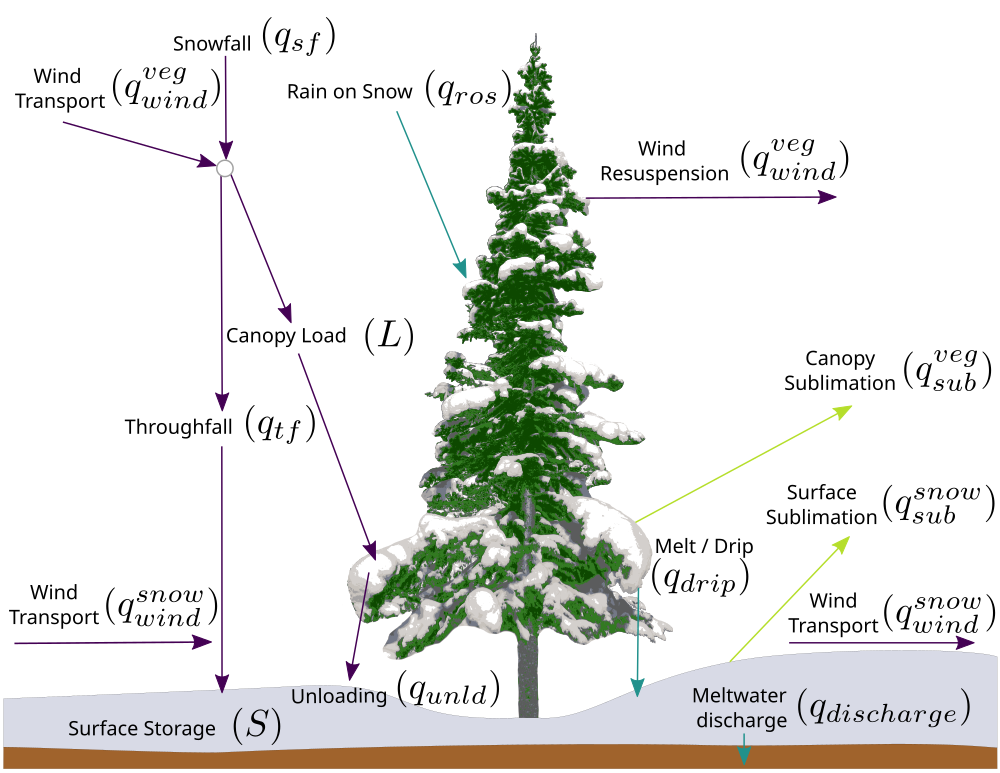
\includegraphics[keepaspectratio]{chapters/02-review-paper/figs/figure1.png}}

}

\caption{\label{fig-mass-bal}The mass balance of intercepted snow in a
needleleaf forest canopy and the subcanopy snowpack. The colours of the
arrows correspond to the water phase: solid (purple), liquid (blue) and
vapour (light green). The head of the arrow indicates a positive flux
either into the canopy (positive) or away from the canopy (negative).
Fluxes may transition between positive and negative. In the case of
sublimation from the canopy or snowpack, the flux may be positive
(sublimation) or negative (deposition). This figure was adapted from
Pomeroy and Gray (1995).}

\end{figure}%

The rate of snow in the canopy undergoing phase change,
\(q_{melt}^{veg}\) (kg m\textsuperscript{-2} s\textsuperscript{-1}), may
be calculated as:

\begin{equation}\phantomsection\label{eq-canopy-snowmelt}{
q_{drip} \approx q_{melt}^{veg} = \frac{Q_{melt}^{veg}}{\lambda_{fus} B}
}\end{equation}

where \(\lambda_{fus}\) (J kg\textsuperscript{-1}) is the latent heat of
fusion, \(B\) is the fraction of ice in a unit mass of wet snow (usually
taken as 0.95-0.97, Gray \& Landine (1988)).

The liquid meltwater output from snow intercepted in the canopy,
\(q_{drip}\) (kg m\textsuperscript{-2} s\textsuperscript{-1}) may be
assumed to be approximately equal to \(q_{melt}^{veg}\) once the snow
has reached its water holding capacity. \(Q_{melt}^{veg}(L)\) (W
m\textsuperscript{-2}) is the rate of energy available to melt canopy
snow which is a function of \(L\). The processes influencing
\(Q_{melt}^{veg}(L)\) are shown in
Equation~\ref{eq-canopy-energy-flux-mp15}.

The rate of sublimation from snow intercepted in the canopy,
\(q_{sub}^{veg}\) (kg m\textsuperscript{-2} s\textsuperscript{-1}) is
determined by the latent heat flux, \(Q_{l}^{veg}\) (W
m\textsuperscript{-2}). Thus, the sublimation rate of snow intercepted
in the canopy may be calculated as (Stull, 2017, eq. 4.45):

\begin{equation}\phantomsection\label{eq-lsub}{
q_{sub}^{veg}(L) = \frac{Q_{l}^{veg}}{\lambda_{sub}}
}\end{equation}

where \(\lambda_{sub}\) (J kg\textsuperscript{-1}), is the latent heat
required for sublimation.

\subsection{Energy Balance}\label{energy-balance}

The processes providing energy available for, \(Q_{melt}^{veg}(L)\), or
the rate of change of the bulk temperature of all constituents of
vegetation, liquid water and snow,
\(\frac{\partial T^{veg}}{\partial t}\) (K s\textsuperscript{-1}) are
shown in Figure~\ref{fig-canopy-energy-balance}. The notation in
Figure~\ref{fig-canopy-energy-balance} and in
Equation~\ref{eq-canopy-energy-flux-mp15} uses superscripts to specify
which control volume the flux refers to: the vegetation control volume
(veg), the snow-atmosphere interface (sai), and the top of the canopy
between the upper atmosphere and canopy air space (total).
Figure~\ref{fig-canopy-energy-balance} shows the canopy air space which
is a control volume used by some models (e.g., Clark et al. (2015a)) to
differentiate the atmospheric conditions within and above the forest
canopy.

The energy balance of the canopy is typically solved using a bulk
approach in hydrological models which treats the canopy as a mixture of
air, water, snow, ice, stems, and leaves (Clark et al. (2015b); Ellis et
al. (2010); Parviainen \& Pomeroy (2000)):

\begin{equation}\phantomsection\label{eq-canopy-energy-flux-mp15}{
Q_{melt}^{veg}(L) = 
Q_{sw}^{veg} +
Q_{lw}^{veg} +
Q_{p}^{veg} + Q_{h}^{veg} - Q_{l}^{veg} - C_p^{veg} \frac{\partial T^{veg}}{\partial t} D_{can}
}\end{equation}

where \(C_p^{veg}\) (J m\textsuperscript{-3} K\textsuperscript{-1}) is
the volumetric bulk storage capacity for heat of all constituents of
vegetation, liquid water and snow, \(D_{can}\) (m) is the depth of the
vegetation canopy, \(Q_{sw}^{veg}\) and \(Q_{lw}^{veg}\) (W
m\textsuperscript{-2}) are the net shortwave and longwave radiation heat
fluxes to the canopy, \(Q_p\) (W m\textsuperscript{-2}) is the advective
energy rate, which may include energy added to the canopy by
\(q_{ros}\), and \(Q_{l}^{veg}\) and \(Q_{h}^{veg}\) (W
m\textsuperscript{-2}) are the turbulent fluxes of latent heat and
sensible heat, respectively, from the vegetation elements to the canopy
air space. A negative value corresponds to a transfer of energy away
from the vegetation elements.

\begin{figure}

\centering{

\pandocbounded{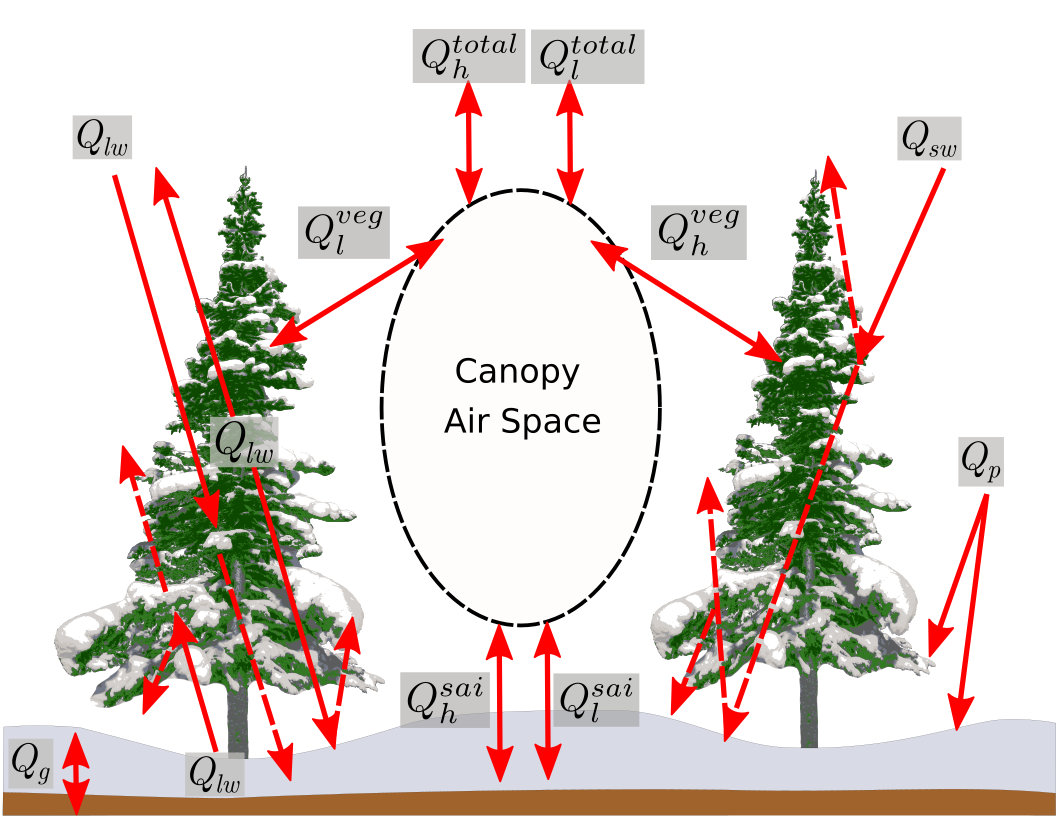
\includegraphics[keepaspectratio]{chapters/02-review-paper/figs/figure2.png}}

}

\caption{\label{fig-canopy-energy-balance}Conceptual representation of
the physical processes important in the energy balance of the forest
canopy and surface snowpack. Where \(Q_{sw}\) and \(Q_{lw}\) (W
m\textsuperscript{-2}) are shortwave and longwave fluxes, \(Q_{l}\) and
\(Q_{h}\) (W m\textsuperscript{-2}) are the turbulent fluxes of latent
heat and sensible heat, \(Q_p\) (W m\textsuperscript{-2}) is the
advective energy rate, and \(Q_p\) (W m\textsuperscript{-2}) is the
ground heat flux. A superscript specifies which control volume the flux
refers to: the vegetation control volume (veg), the snow-atmosphere
interface (sai), and the top of the canopy between the upper atmosphere
and canopy air space (total). The dashed lines represent radiation
extinguished, reflected or re-emitted by the canopy, intercepted snow or
surface snowpack. This figure was adapted from Clark et al.~(2015a).}

\end{figure}%

With Equation~\ref{eq-canopy-energy-flux-mp15}, for a cold canopy
snowpack (\(T^{veg}\) \textless{} 0°C), all energy goes into warming the
control volume (increasing \(\frac{\partial T^{veg}}{\partial t}\)) and
no melt of canopy snow occurs (warming phase, \(T^{veg}\) = 0). Once
\(T^{veg}\) reaches 0°C, \(Q_{melt}^{veg}(L)\) increases as more energy
becomes available for melt and \(\frac{\partial T^{veg}}{\partial t}\)
equals zero (ripening and output phase) assuming the temperature of
canopy snow is equal to that of the canopy when \(T^{veg}\) \textless=
0°C.

\section{Measurement Techniques}\label{sec-methods}

\subsection{Weighed Tree}\label{weighed-tree}

Weighed tree lysimetry is one of the few direct methods to quantify the
amount of snow intercepted in and ablated from the canopy. A cut tree is
either weighed from a load cell on the ground (Lundberg \& Halldin,
1994; e.g., Schmidt et al., 1988; Storck et al., 2002; Watanabe \&
Ozeki, 1964) or an inline strain gauge suspended from the crown of the
tree as shown in Figure 3 (Hedstrom \& Pomeroy, 1998; e.g., Pomeroy et
al., 1993). To scale the weight of snow in the canopy (kg) to per unit
area (kg m\textsuperscript{-2}), there are two methods described in the
literature. Katsushima et al. (2023), Satterlund \& Haupt (1967), and
Watanabe \& Ozeki (1964) estimated the projected crown area
(m\textsuperscript{2}) of the weighed tree to convert weighed tree
measurements in weight (kg) to snow load per unit area (kg
m\textsuperscript{-2}). Pomeroy et al. (1993) and Hedstrom \& Pomeroy
(1998), calculated areal estimates of \(\frac{dL}{dt}\), using the mass
balance method described in Section~\ref{sec-mass-bal-methods} along
with fresh snow survey measurements of throughfall and point
measurements of \(q_{sf}\), to relate the weight change measured by the
weighed tree to a per-unit-area measurement of \(\frac{dL}{dt}\).
Although the weighed tree method offers a direct measurement of
\(\frac{dL}{dt}\), it is limited to a point scale and can be
impracticable for very tall trees due to challenges in constructing a
tree mounting system. During periods of snowfall, \(\frac{dL}{dt}\)
measured by the weighed tree is attributed to intercepted snowfall and
ablation (Equation~\ref{eq-canopy-mass-bal}). In the absence of
\(q_{sf}\) and hence \(q_{tf}\) and \(q_{ros}\), the change in canopy
snow load can be attributed to the remaining processes in
Equation~\ref{eq-canopy-mass-bal}.

\begin{figure}

\begin{minipage}{0.50\linewidth}

\centering{

\pandocbounded{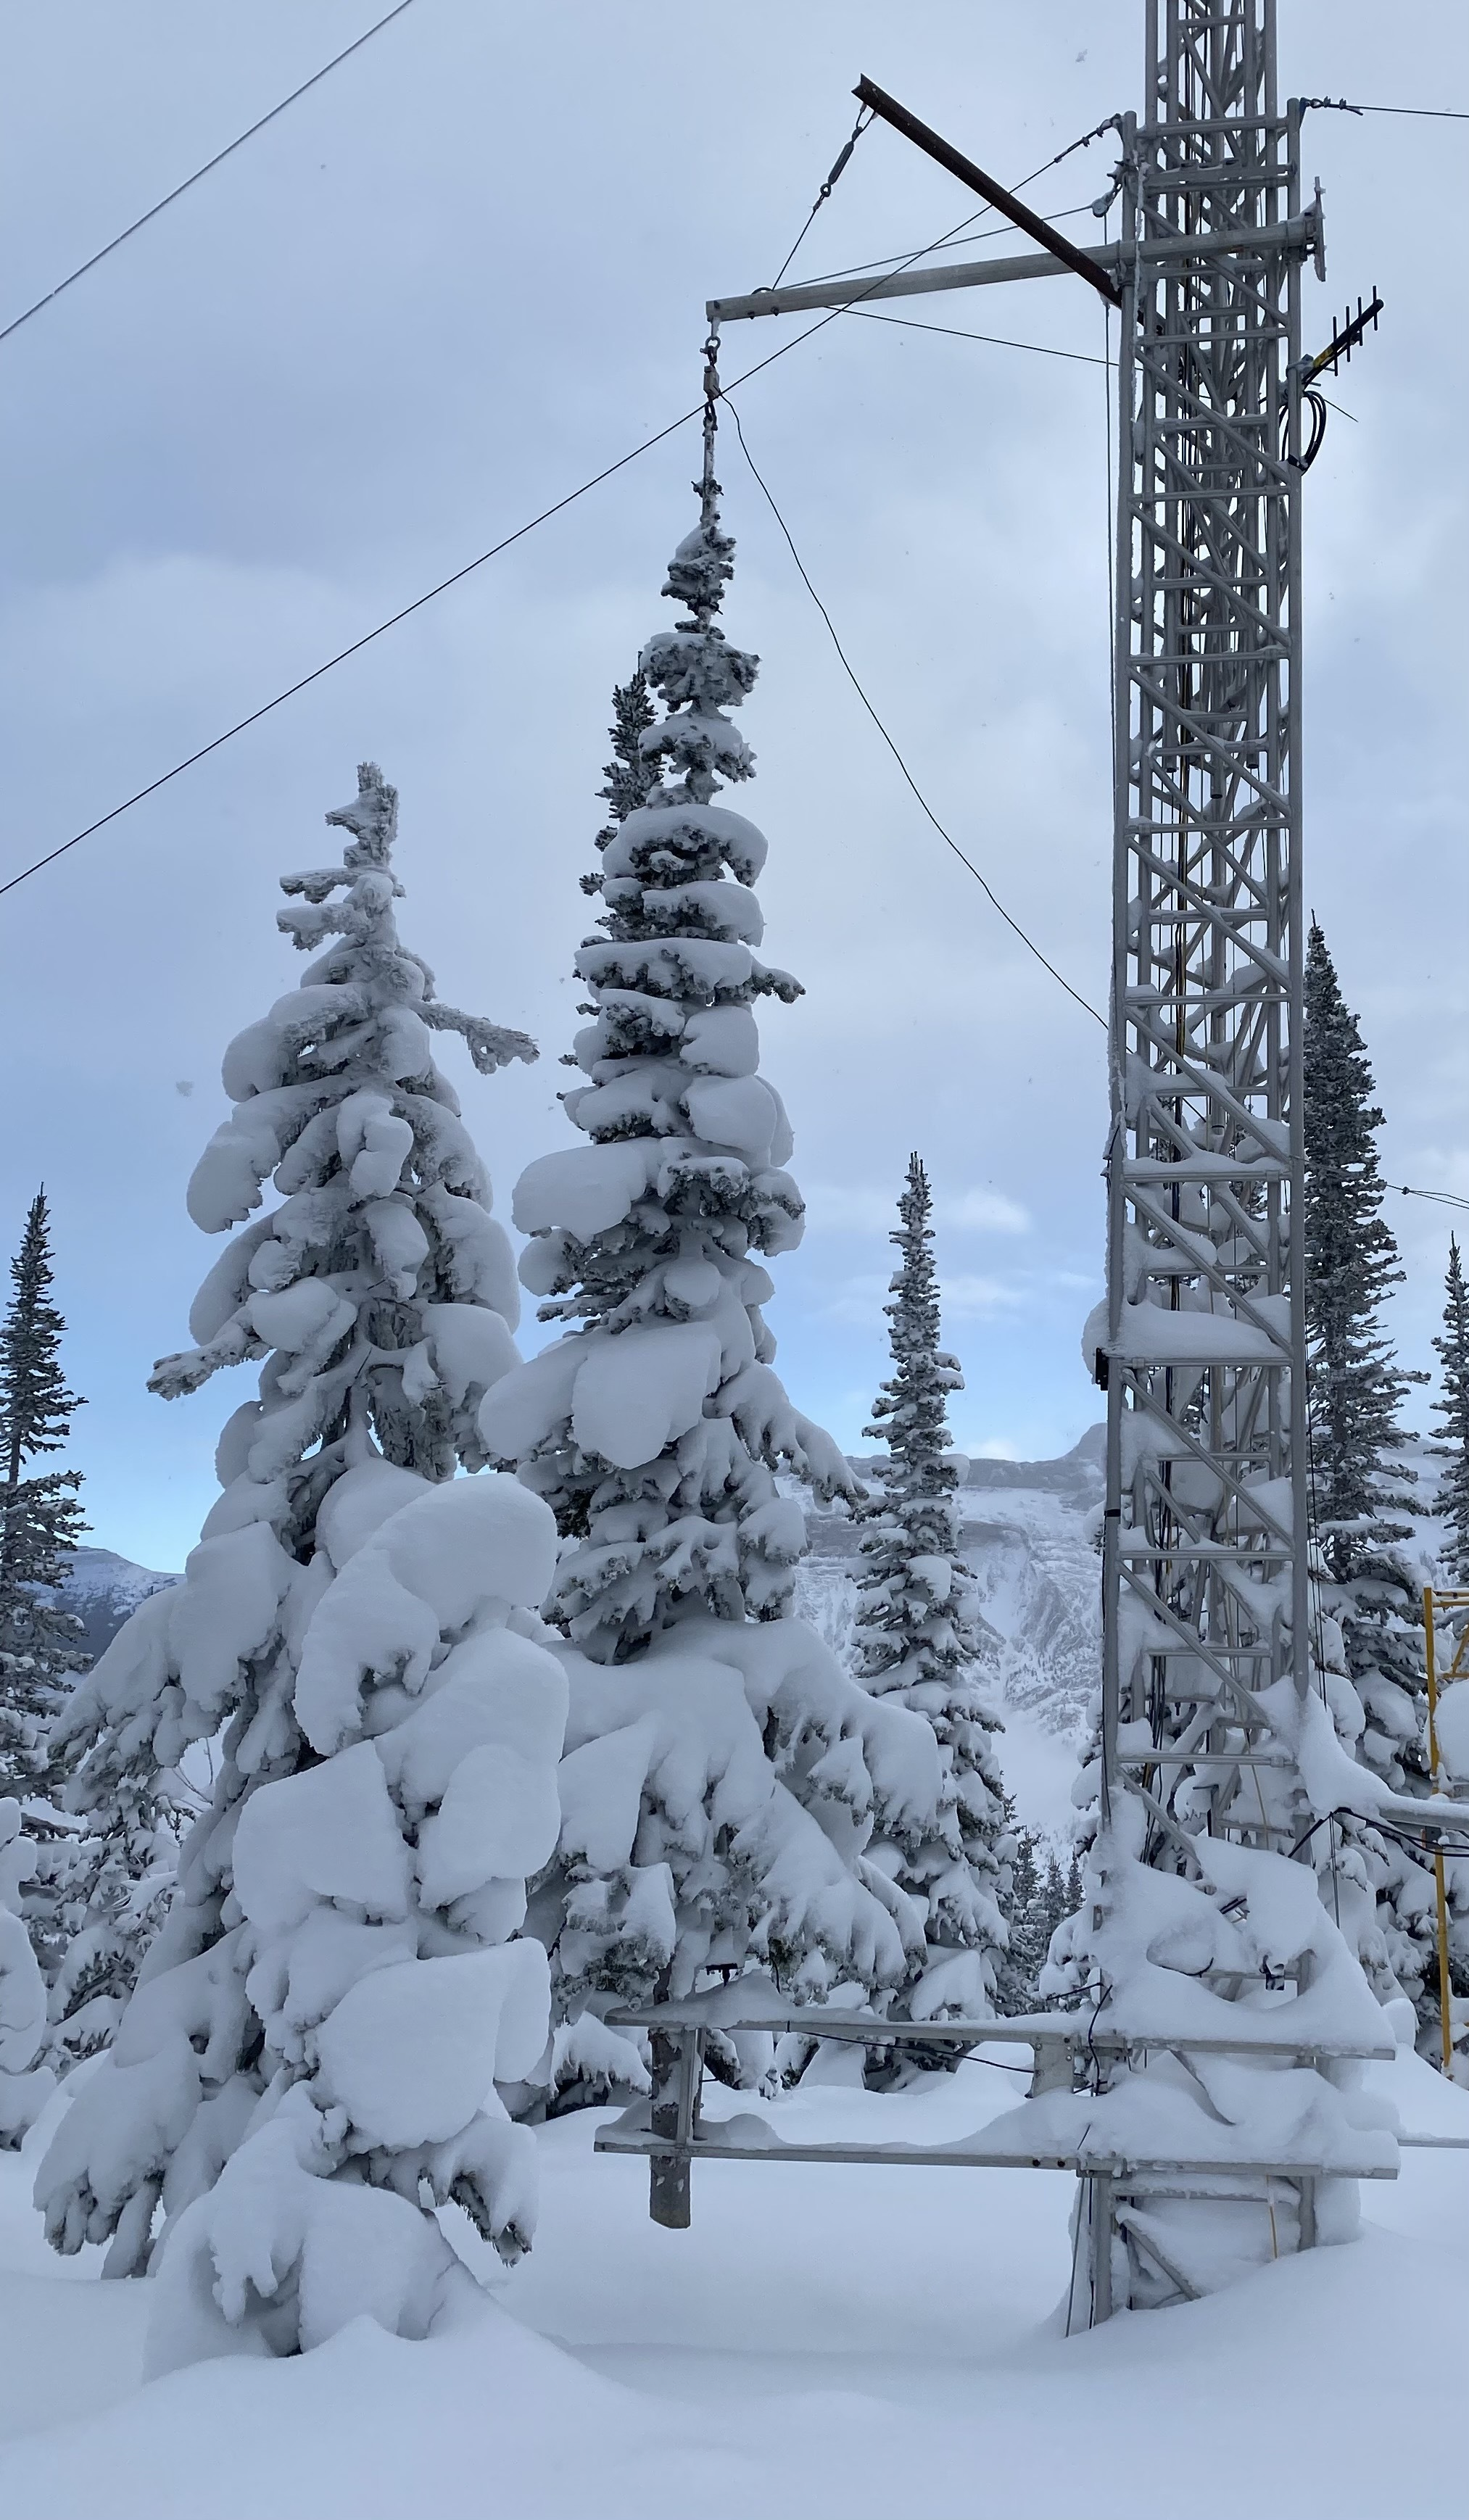
\includegraphics[keepaspectratio]{chapters/02-review-paper/figs/figure3a.jpg}}

}

\subcaption{\label{fig-w-tree-loaded}}

\end{minipage}%
%
\begin{minipage}{0.50\linewidth}

\centering{

\pandocbounded{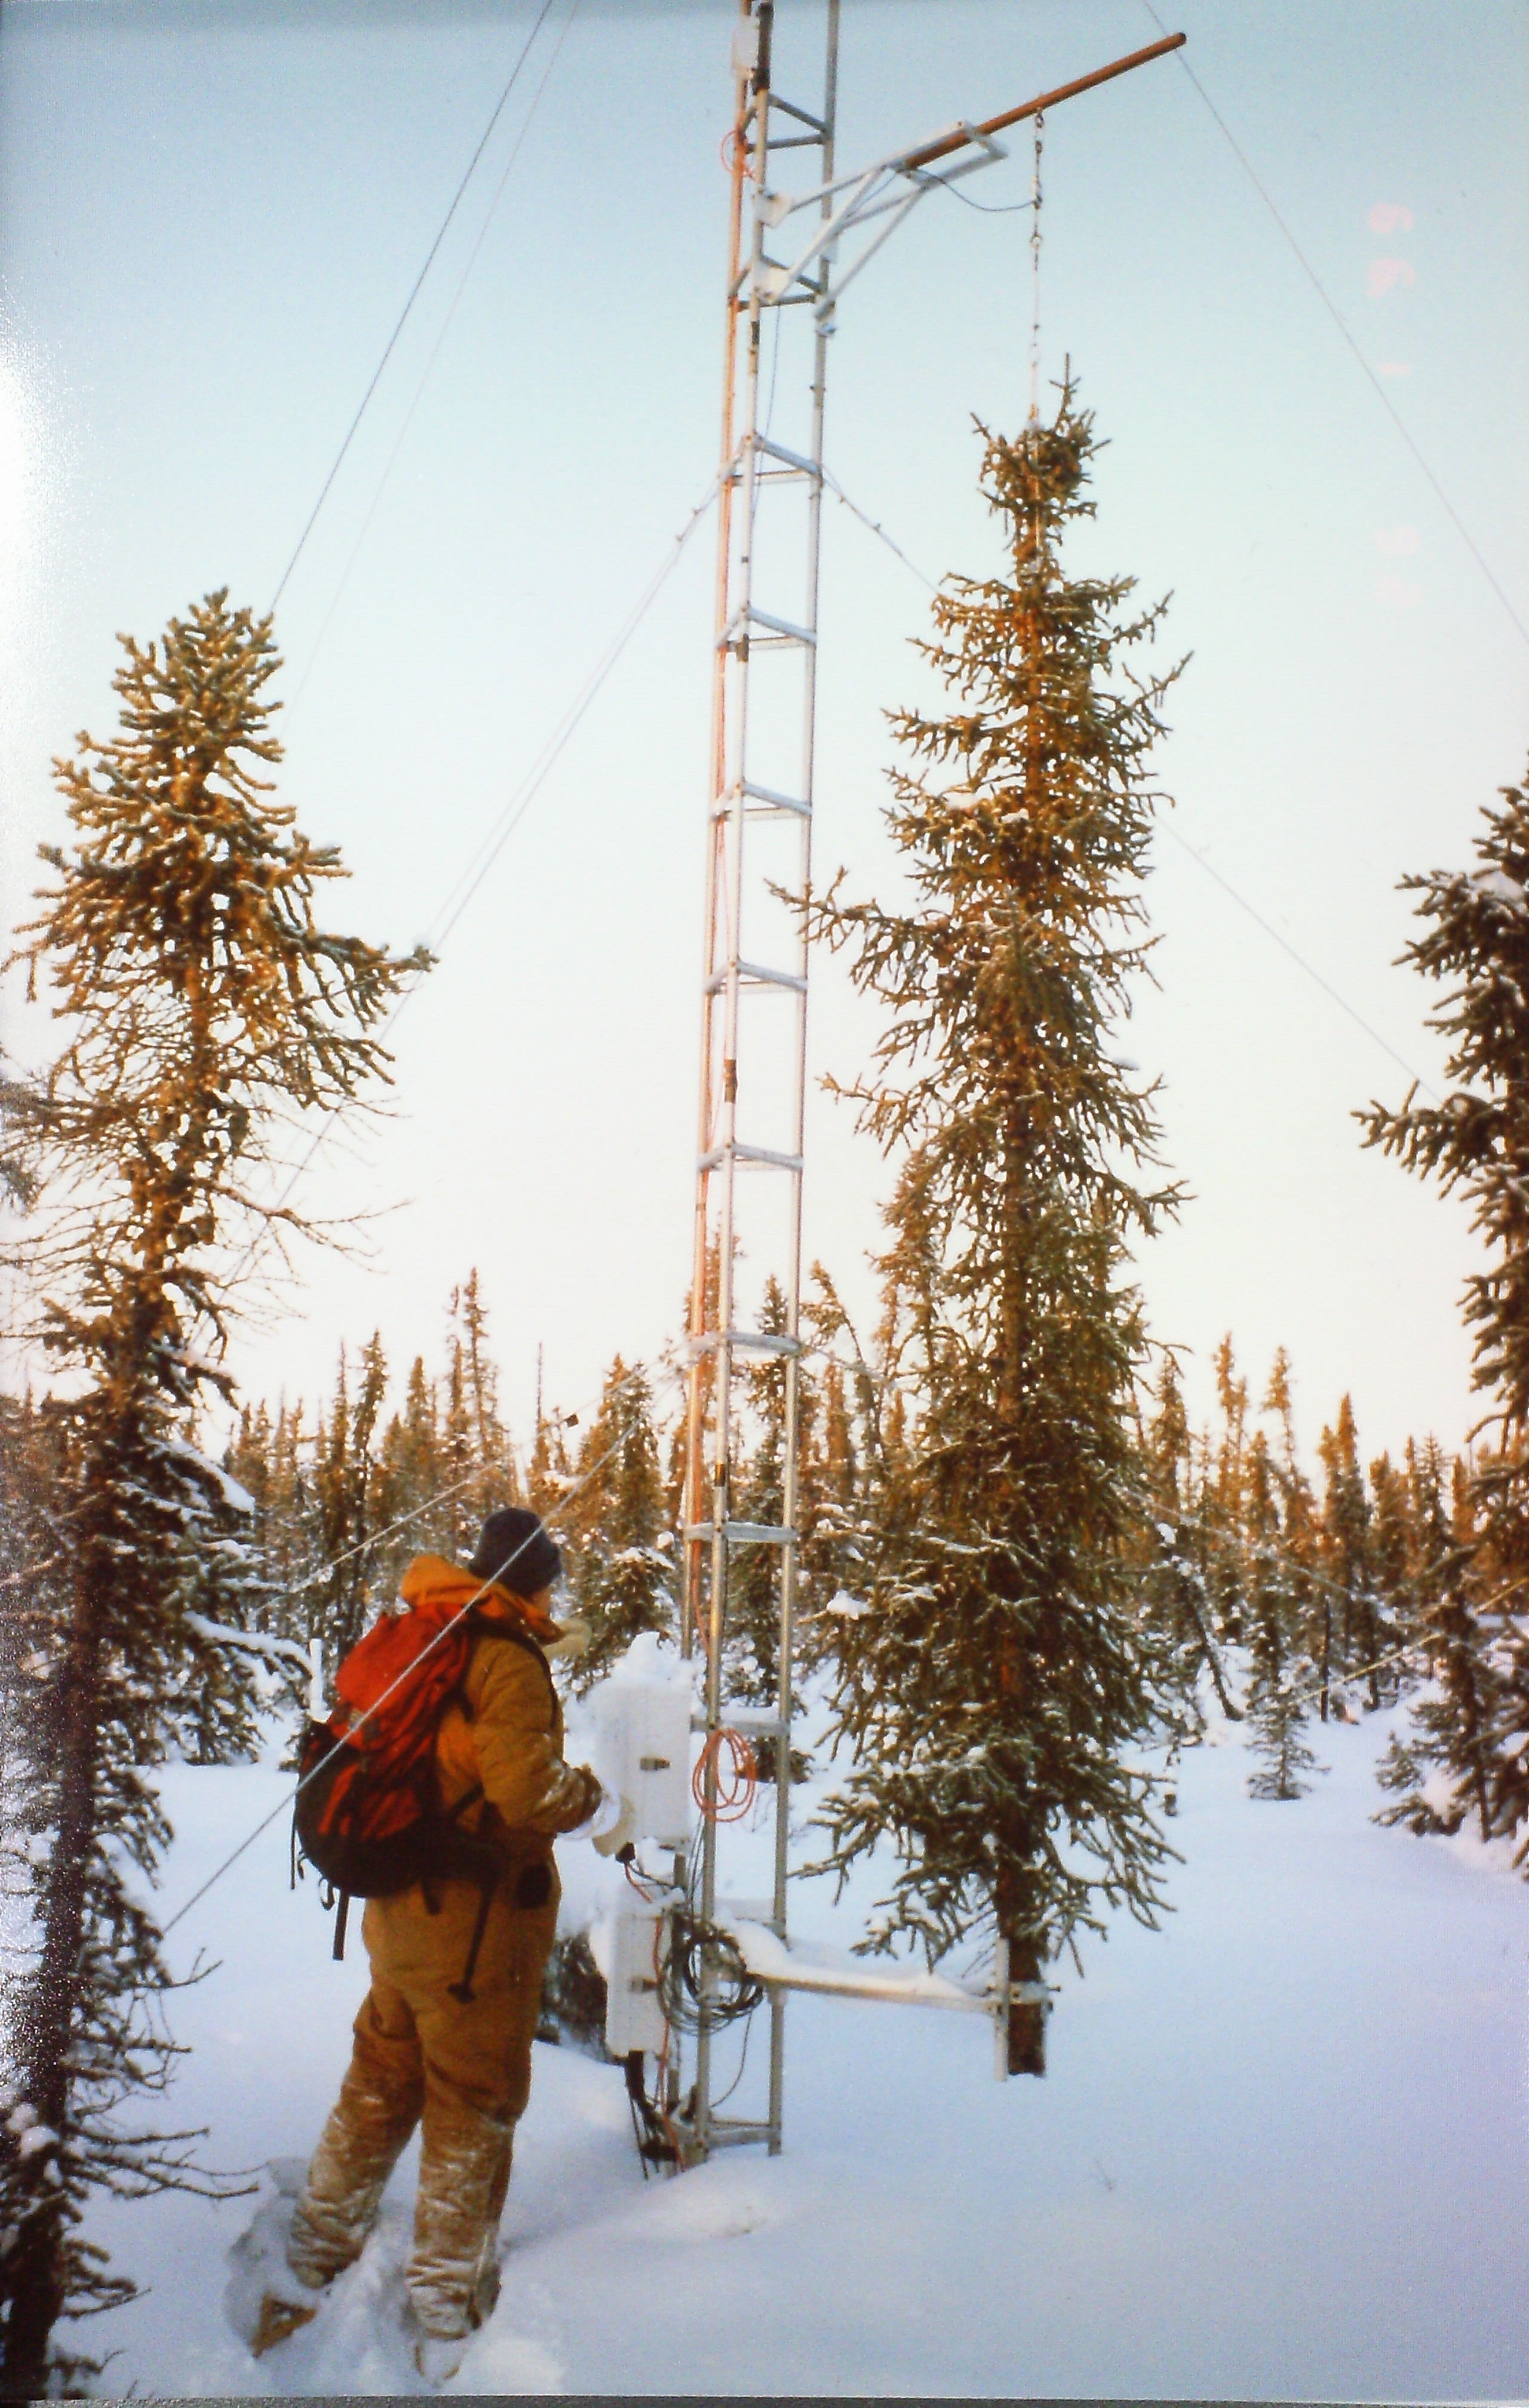
\includegraphics[keepaspectratio]{chapters/02-review-paper/figs/figure3b.jpg}}

}

\subcaption{\label{fig-w-tree-bare}}

\end{minipage}%

\caption{\label{fig-insts}Weighed tree lysimeters, (a) Subalpine fir
tree lysimeter loaded with snow, Fortress Mountain Research Basin,
Alberta, Canada and (b) Black spruce tree lysimeter relatively free of
snow, Havikpak Creek Research Basin, Inuvik, Northwest Territories,
Canada.}

\end{figure}%

\subsection{Mass Balance Methods}\label{sec-mass-bal-methods}

Since \(L\) is difficult to measure over spatial and temporal time
scales, throughfall measurements can be used to infer canopy snow load
as a residual based on Equation~\ref{eq-canopy-mass-bal}. If the
assumption is made during snowfall periods with calm winds and cool air
temperatures that ablative processes are negligible,
Equation~\ref{eq-canopy-mass-bal} can be simplified to:

\begin{equation}\phantomsection\label{eq-dwdt-ode}{
\frac{dL}{dt} = q_{sf}-q_{tf}(L)
}\end{equation}

Over a discrete time interval, \(\Delta t\), the change in canopy snow
load, \(\Delta L\) (kg m\textsuperscript{-2}) may be calculated as:

\begin{equation}\phantomsection\label{eq-dwdt-discrete}{
\frac{\Delta L}{\Delta t} = \overline{q_{sf}}-\overline{q_{tf}(L)} = \frac{\Delta sf}{\Delta t} - \frac{\Delta tf}{\Delta t}
}\end{equation}

where \(\overline{q_{sf}}\) and \(\overline{q_{tf}(L)}\) are the average
snowfall and throughfall rate over \(\Delta t\). \(\Delta sf\) and
\(\Delta tf\) is the accumulated above canopy snowfall (kg
m\textsuperscript{-2}) and throughfall respectively.

Throughfall measurements of snow differ from rainfall measurements of
throughfall which typically include \(q_{drip}\) (Van Stan et al.,
2020). However, even for snowfall events with cold temperatures and calm
winds, ablative processes are likely non-zero and thus true measurements
of throughfall are difficult to ascertain.

\subsubsection{Snow Surveys}\label{sec-snow-surveys}

Snow surveys conducted below the canopy are one method to provide areal
estimates of \(\frac{\Delta tf}{\Delta t}\). Combined with measurements
of \(\frac{\Delta sf}{\Delta t}\), Equation~\ref{eq-dwdt-discrete} can
be used to estimate \(\frac{\Delta L}{\Delta t}\). Throughfall depths
may be converted to SWE using observed relationships between snow depth
and snow density (e.g., Staines \& Pomeroy, 2023) or modelled using
empirical equations (e.g., Lv \& Pomeroy, 2020). If the covariance
between snow depth and density is found to be insignificant, Pomeroy \&
Gray (1995) recommend calculating SWE as:

\begin{equation}\phantomsection\label{eq-sweins}{
\frac{\Delta tf}{\Delta t} = \overline{\rho_s} \cdot \frac{d_{ tf}}{\Delta t}
}\end{equation}

where \(\overline{\rho_s}\) is the average snow density over the snow
survey and \(d_{tf}\) is the depth of throughfall (m). \(d_{tf}\) may be
determined using the difference in post-event and pre-event snow depth
using rulers (e.g., Hedstrom \& Pomeroy, 1998), or using aerial lidar
derived surface models (e.g, Staines \& Pomeroy, 2023). Uncertainties
with these two methods include penetration of the ruler into the soil
which falsely increases the snow depth, and errors associated with lidar
methods of 5---20 cm (RMSE) described in Harder et al. (2020) and
Staines \& Pomeroy (2023). If a defined layer (i.e., natural ice crust
or measurement plate) is present prior to a snowfall event, depths of
snow above this layer may be taken as \(d_{tf}\) as in Moeser et al.
(2015b). Automated acoustic snow depth sensors have also been used to
measure \(d_{tf}\) as the difference in the change in snow depth to an
open area and subcanopy (Lv \& Pomeroy, 2020; Roth \& Nolin, 2019).
Regardless of the method chosen, care must be taken to ensure ablation
of snow in the canopy and on the ground is minimal over the snowfall
period to ensure Equation~\ref{eq-dwdt-discrete} is valid.

\(\rho_s\) may be measured using gravimetric fresh snow density
sampling. With this method a pit is dug to below the bottom of the new
throughfall layer and a snow density sampler of a known volume is pushed
horizontally into the new snow layer (e.g., Figure~\ref{fig-fsd}) and
the resulting sample is weighed. Additional methods are available for
the calculation of snow density including snow tubes, microwave radar,
gamma ray, snow pillow, and snow scale. However, these methods have
constraints in providing a density of a new snow layer and are more
commonly applied to measure density of the entire snowpack to the
ground.

\begin{figure}

\centering{

\pandocbounded{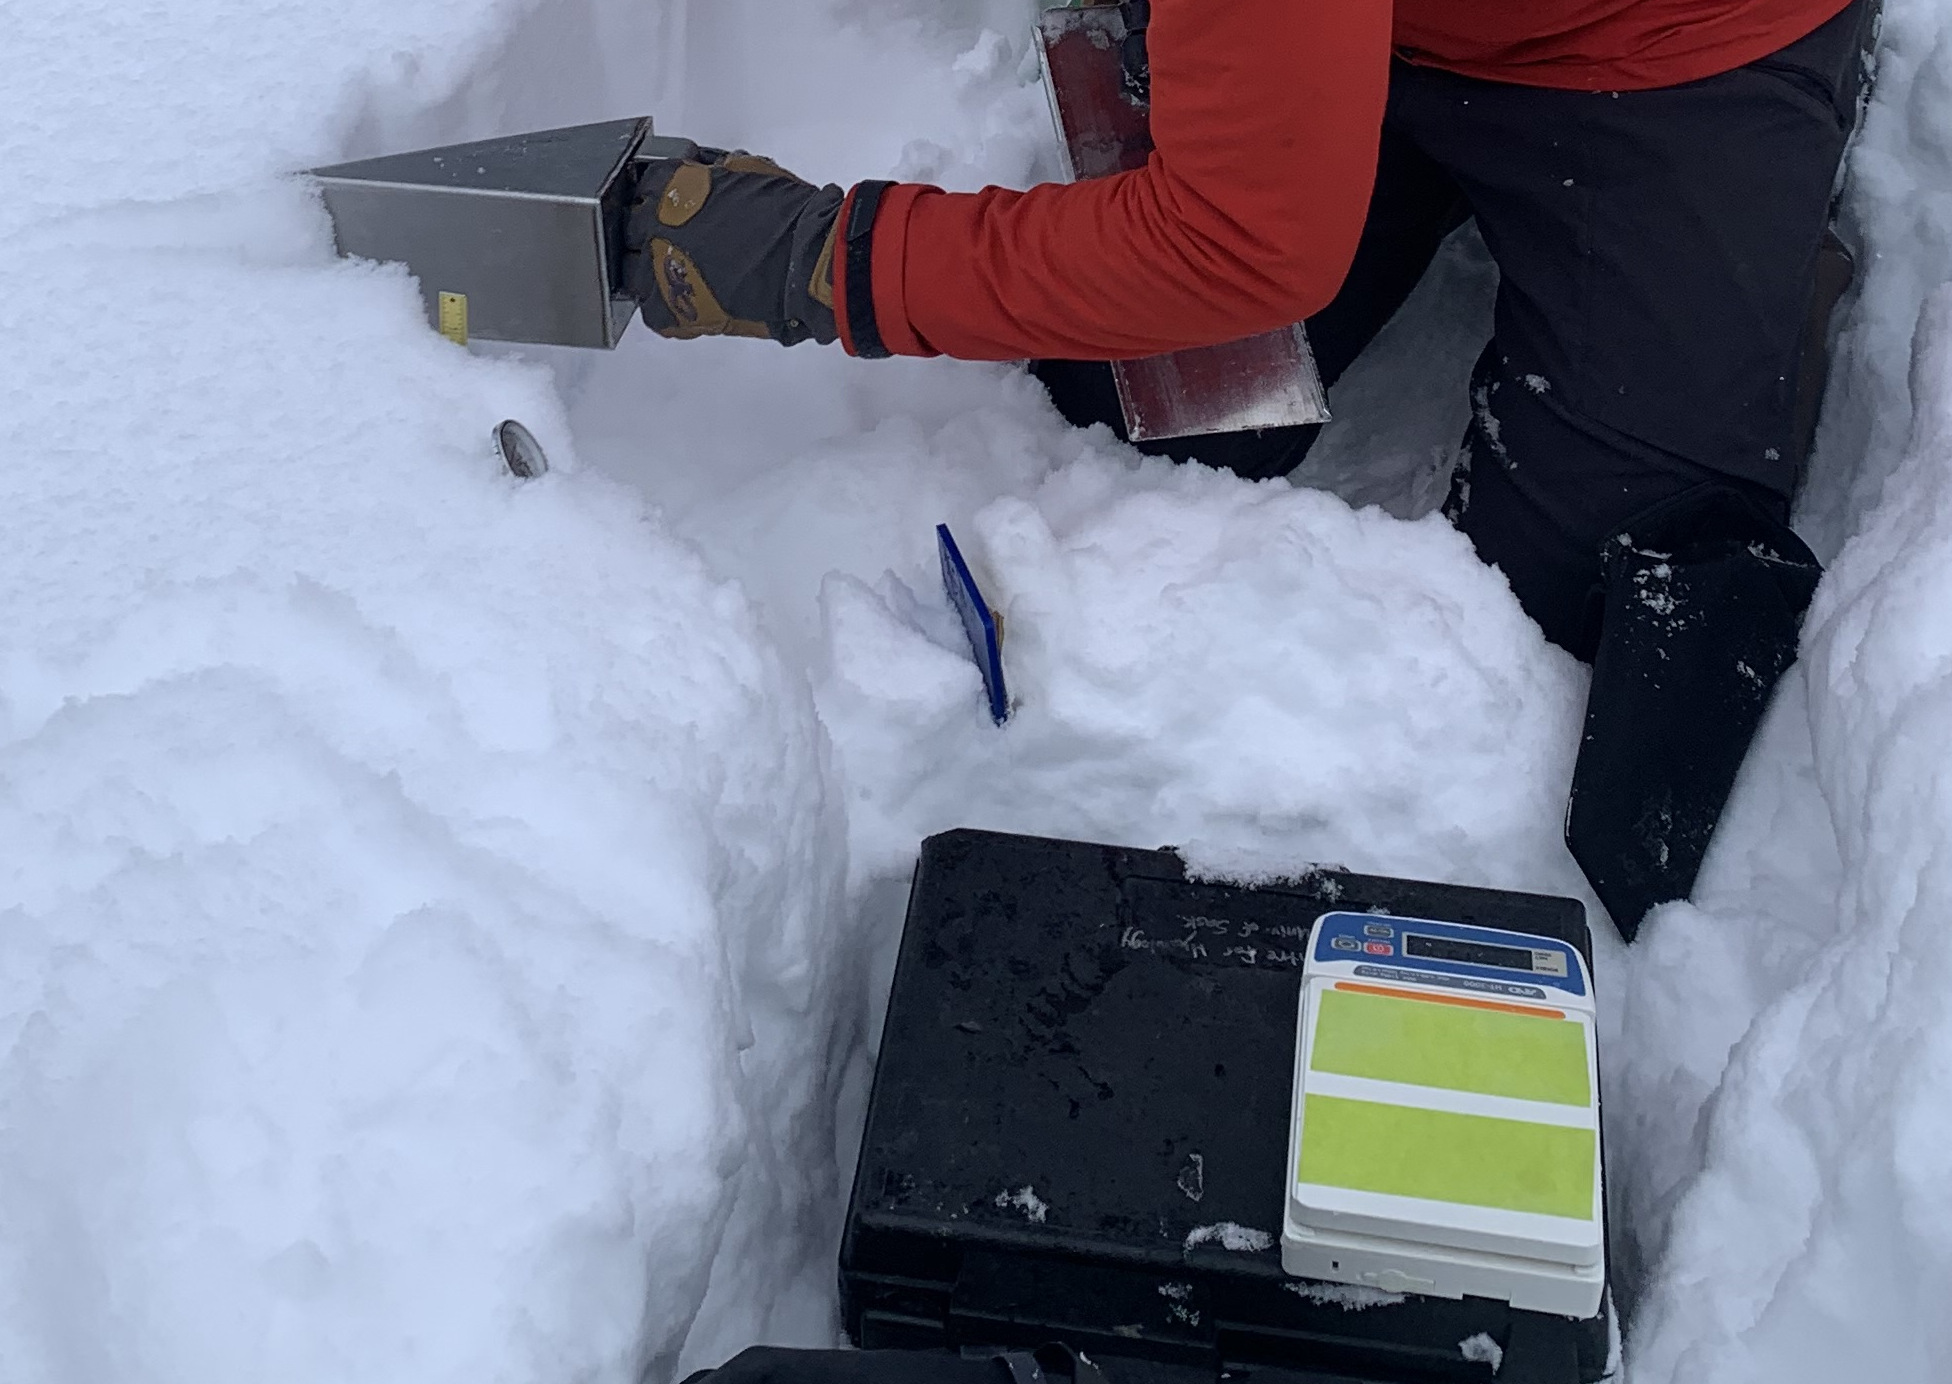
\includegraphics[keepaspectratio]{chapters/02-review-paper/figs/figure4.jpg}}

}

\caption{\label{fig-fsd}Gravimetric fresh snow density sample
collection, Fortress Mountain Research Basin, Alberta, Canada. A 1000
cm3 snow density wedge sampler (RIP Cutter,
https://snowmetrics.com/shop/rip-1-cutter-1000-cc/) is shown being
pushed into the surface of the snowpack. The scale used to measure the
weight of the sample is shown on the bottom right.}

\end{figure}%

\subsubsection{Subcanopy Lysimeters}\label{subcanopy-lysimeters}

Subcanopy lysimeters may provide measurements of \(\overline{q_{tf}}\)
and/or the downward ablation of snow in the canopy,
\(\overline{q_{unld}}\) and \(\overline{q_{drip}}\). When paired with an
automated data logger, measurements can be taken over relatively shorter
discrete time intervals compared to manual snow surveys. With this
method, a trough or bucket is suspended from a load cell (e.g.,
Figure~\ref{fig-scl-2}) or installed on the ground (e.g., Storck et al.,
2002) and measures the accumulated weight (kg) of snow entering the
lysimeter. The surface area of the opening of the trough is used to
convert the weight to a per unit area measurement in (kg
m\textsuperscript{-2}). For periods where, \(q_{unld}\) and \(q_{drip}\)
can be considered negligible, the subcanopy lysimeters provide
measurements of \(\overline{q_{tf}} \Delta t\) and using
Equation~\ref{eq-dwdt-discrete} along with
\(\overline{q_{sf}} \Delta t\) can be used to estimate
\(\frac{dL}{dt}\). For periods without snowfall, the subcanopy
lysimeters provide measurement of \(q_{unld}+q_{drip}\).

\begin{figure}

\centering{

\pandocbounded{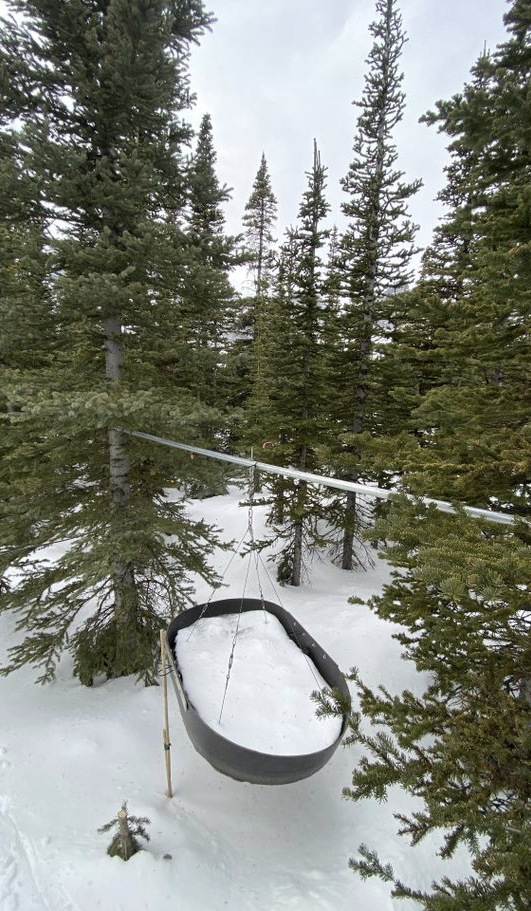
\includegraphics[keepaspectratio]{chapters/02-review-paper/figs/figure5.jpg}}

}

\caption{\label{fig-scl-2}An example of a suspended subcanopy lysimeter
installed at Fortress Mountain Research Basin, Alberta, Canada to
measure rates of throughfall, unloading, and drip.}

\end{figure}%

Measurements of \(q_{drip}\) are difficult to ascertain due to its
simultaneous occurrence with \(q_{unld}\) especially in warm
temperatures. To isolate, \(q_{drip}\), researchers(e.g., Floyd, 2012;
Storck et al., 2002) have utilized tipping bucket rainfall gauges
positioned beneath the canopy to quantify the drainage rate of liquid
water from snow intercepted in the canopy. However, employing tipping
buckets in temperatures close to 0°C presents difficulties as the
mechanical apparatus can freeze, resulting in missed measurements. The
simultaneous occurrence of \(q_{unld}\) during the melt process may
provide an additional source of liquid water as ripe clumps of snow
continue to melt into the tipping bucket device. The difficulty in
isolating the multiple processes, as outlined in
Equation~\ref{eq-canopy-mass-bal} and Figure~\ref{fig-mass-bal}, that
contribute snow beneath the canopy is the main limitation of using
subcanopy lysimeters to measure snow interception and canopy snow
ablation. Therefore, use of this methodology should be paired with other
observations such as meteorological measurements, timelapse imagery or a
weighed tree to help determine if unloading and drip are likely.

\subsection{Remote Sensing}\label{remote-sensing}

Remote sensing methodologies have proven effective in acquiring
measurements of throughfall, canopy snow load, and ablation over larger
spatial extents and more frequent temporal scales compared to the
measurements discussed above (Bartlett \& Verseghy, 2015; Calder, 1990;
Floyd \& Weiler, 2008; Russell et al., 2020). For example, Calder (1990)
used a gamma ray attenuation system to continuously measure canopy snow
load within a forest plot. However, the gamma ray technique has not been
repeated in canopy-scale snow interception studies due to the danger of
emissions from the radioactive source. Aside from the study conducted by
Calder (1990), remote sensing methods generally do not directly measure
canopy snow load in units of kg m\textsuperscript{-3}. Instead, they
provide a volumetric measurement of canopy load, a measurement of
throughfall, an index based on above canopy albedo, or an areal fraction
of canopy covered by snow.

One volumetric approach, as demonstrated by Russell et al. (2020),
utilized autonomous terrestrial laser scanning (ATLS) to measure the
volume of snow intercepted in the canopy. This method involves
collecting ATLS point clouds for an individual tree during snow-free and
snow-on conditions. The 3D approximations created from these point
clouds are used to calculate the canopy volume for both conditions,
while also accounting for branch bending and lidar beam occlusion. By
subtracting the snow-on volume from the snow-free volume, an estimate of
the snow intercepted in the canopy is obtained. Limitations with the
ATLS method include challenges such as changes in tree geometry under
snow loading and lidar beam occlusion which were only partially
addressed by the Russell et al. (2020) method, and the difficulty of
estimating the density of intercepted snow in the canopy. These
challenges contributed to the weak correlation observed by Russell et
al. (2020) when comparing results with measurements of canopy snow load
obtained through weighed tree assessments. Indirect measurements of
canopy snow load using aerial lidar throughfall measurements are
discussed in Section~\ref{sec-snow-surveys}.

The studies conducted by Roesch et al. (2001) and Bartlett \& Verseghy
(2015) utilized measurements of above canopy albedo, which is
hypothesised to increase as snow is intercepted in the canopy and reduce
light transmittance through the canopy. However, given the potential for
fresh snowfall to cover the upward-facing radiometer and lead to
erroneous albedo measurements, cleaning radiometers following snowfall
events is crucial. A study using radiometer measurements that were
cleaned after each snowfall event, by Nakai et al. (1999) highlights
that very large canopy snow loads show an increase in above canopy
albedo. For small snow loads (\textless{} 1.6 kg m\textsuperscript{-2})
Pomeroy \& Dion (1996) show that no relationship was found between
canopy snow load and above canopy albedo over a mature pine canopy using
a frequently cleaned radiometer. More recent work by Lv \& Pomeroy
(2019) shows that the normalised snow difference index calculated using
Landsat satellite imagery dramatically increased with canopy snow load.
Lv \& Pomeroy (2019) also show a small, but detectable increase in
albedo was found when the canopy was covered with snow. This method has
limitations for smaller snowfall events in some tree species and canopy
structures Pomeroy \& Dion (1996) or when radiometer measurements are
erroneous.

Time-lapse photography has been an important component of understanding
canopy snow processes at the plot or individual tree scale since early
work by Berndt \& Fowler (1969) to quantify rime accretion on needleleaf
canopy. Pomeroy et al. (1993) developed perimeter-area relationships to
quantify the sublimation rate of intercepted snow, using photographs and
fractal geometry, but found no unique relationship between oblique
snow-covered canopy fraction, measured using digital images and Java
image analysis software, and the mass of snow weighed on a suspended
tree. A method to determine the snow-covered fraction of the canopy was
developed by Floyd \& Weiler (2008) using automated image analysis who
noted limitations of this method due to condensation/frost build up on
the camera lens and lighting conditions. Similar methodologies have also
been utilized by several other studies to understand canopy-snow
processes (Dong \& Menzel, 2017; Garvelmann et al., 2013; Parajka et
al., 2012). Recent work by Lumbrazo et al. (2022) involved citizen
scientists to classify time-lapse images of snow in the canopy into an
index of canopy snow-covered fraction to diagnose canopy snow ablation
process models. Additionally, Harvey et al. (2025) show that a deep
learning convolutional neural network model provided estimates of canopy
snow presence from time-lapse imagery that had very close agreement to
images analyzed by humans and also much better accuracy than the
automated thresholding methods used by previous studies.

\subsection{Tree Sway Frequency}\label{tree-sway-frequency}

The sway frequency of trees has been shown to decrease proportionally
with increasing mass stored in the canopy (Papesch, 1984; Raleigh et
al., 2022). A study by Raleigh et al. (2022) utilized a
three-dimensional accelerator attached to the upper section of a tree to
quantify wind induced movements and provide an index of canopy snow
load. Raleigh et al. (2022) showed that the influence of thermal effects
on tree rigidity must be considered when analyzing sway frequency in
cold climates. Raleigh et al. (2022) notes additional challenges with
this method including difficulties in isolating a separate relationship
for tree sway frequency and thermal effects and relating changes in sway
frequency to changes in snow load. Schmidt \& Pomeroy (1990) show that
the modulus of elasticity of tree branches varies with temperature below
0°C, indicating this technique is strongly impacted by freezing and
thawing of trunks. Measurements of canopy snow load are also limited to
periods of heightened wind where canopy snow is also likely to ablate.

\subsection{Trunk Compression}\label{trunk-compression}

Measurement of trunk compression, initially utilized for monitoring the
mass of intercepted rain in the canopy (Friesen et al., 2008), has been
adapted for measurement of canopy snow load by Martin et al. (2013).
This method is based on Hooke's law of elasticity to infer a change in
mass through the trunk's compression and expansion. However,
uncertainties with this method include the need for individual
tree-specific calibration for determining the modulus of elasticity.
Additionally, factors such as transpiration, sap flow, wind, and
temperature contribute to noise in the instrumentation, primarily
through thermal expansion and wind induced compression of the trunk. The
expansion and compression of trees with freezing and thawing discussed
by Gutmann et al. (2017) suggests further research is required to apply
this method to freezing trunks. Sensors with extremely high precision (±
1---2 µm) are also required for this method leading to high cost.

\subsection{Eddy Covariance}\label{eddy-covariance}

The rate of canopy snow sublimation, \(q_{sub}^{veg}\) (kg
m\textsuperscript{-2} s\textsuperscript{-1}), can be measured using the
eddy covariance technique (e.g., Harding \& Pomeroy, 1996; Lundberg \&
Halldin, 2001; Molotch et al., 2007; Parviainen \& Pomeroy, 2000). With
this method, an eddy covariance system measures the latent heat flux
above the canopy resulting from evapotranspiration, evaporation, and
sublimation of snow on the surface and in the canopy. During cool
periods where evapotranspiration and evaporation rates are assumed
negligible, the latent heat flux can be attributed to \(Q_l^{sai}\) +
\(Q_l^{veg}\) and can be converted to \(q_{sub}^{snow}\) +
\(q_{sub}^{veg}\) using Equation~\ref{eq-lsub}. A second eddy covariance
system installed beneath the canopy above the surface snowpack to
measure \(Q_l^{sai}\), which can be used to isolate \(Q_l^{veg}\) in the
above canopy latent heat measurements (Molotch et al., 2007).
Alternatively, the subcanopy snowpack sublimation rate may be assumed
negligible, and a single eddy covariance system is used (Lundberg \&
Halldin, 2001; Parviainen \& Pomeroy, 2000). Uncertainties in this
measurement technique stem from assumptions such as negligible
transpiration rates from surrounding vegetation, the requirements of a
homogeneous surface, and slow variations in airflow properties. Many
studies show a failure to close the above canopy energy balance when the
canopy is snow-covered (e.g., Harding \& Pomeroy, 1996). Harvey et al.
(2025) also demonstrated that this method incorrectly identified
\(q_{sub}^{veg}\) for several days when the canopy was observed to be
without snow in time-lapse images. They attributed this to differing
flux footprints of the above and below-canopy eddy covariance
measurements and/or sublimation of wind-suspended snow.

\subsection{Snow Isotopes}\label{snow-isotopes}

Investigating the isotopic composition of water and snow has proven
valuable for understanding hydrological (e.g., Galewsky et al., 2016)
and snow (Beria et al., 2018) processes. During phase changes, snow
undergoes isotopic fractionation, altering the relative abundance of
heavier and lighter isotopes of hydrogen and oxygen among the different
phases. While sublimation of snow intercepted in the canopy is known to
enrich heavier isotopes in the remaining snow (Beria et al., 2018),
relatively few studies have utilized snow isotopes to explore canopy
snow processes (Claassen \& Downey, 1995; Koeniger et al., 2008).
Interpreting isotopic fractionation in canopy snow is challenging, as
fractionation from cold, sublimating snow can be minimal (Schlaepfer et
al., 2014), whilst wet snow undergoing sublimation, deposition, and melt
shows varying degrees of fractionation (Beria et al., 2018).
Additionally, some clumps of snow may completely sublimate while others
partially sublimate or melt, complicating the link between isotope
enrichment and a specific process. Chemical changes in intercepted snow
have been shown by Pomeroy et al. (1999) to present similar
complications on linking chemical changes to individual processes,
limiting its usefulness for quantifying canopy snow mass exchange
processes. Subsequent fractionation also can occur in the subcanopy
snowpack as meltwater percolates and refreezes or the surface snow
sublimates (Beria et al., 2018), which further complicates isolating
specific processes.

\section{Parameterisations}\label{sec-parameterisations}

\subsection{Snow Interception Parameterisations}\label{sec-interception}

Snow interception parameterisations differ in their approximation of the
maximum canopy snow storage capacity (Figure~\ref{fig-example-wmax-ip},
a) and the fraction of snowfall intercepted
(Figure~\ref{fig-example-wmax-ip}, b), due to differences in the
relationships and variables included in each parameterisation
(Table~\ref{tbl-mod-desc}). This leads to large discrepancies in the
predicted canopy snow load shown in Figure~\ref{fig-L-cold-warm} and
thus the amount of snow available for sublimation losses. The factors
contributing to these model discrepancies can be grouped into intrinsic
factors of the vegetative structure (e.g., canopy coverage, leaf area
and surface temperature) and extrinsic factors (e.g., snowfall event
meteorology, methodologies). Parameterisations for snowfall interception
have all been derived for evergreen needleleaf forests and thus
constrain the scope of this section (Hedstrom \& Pomeroy, 1998;
Satterlund \& Haupt, 1967; Storck et al., 2002).

\begin{figure}

\centering{

\pandocbounded{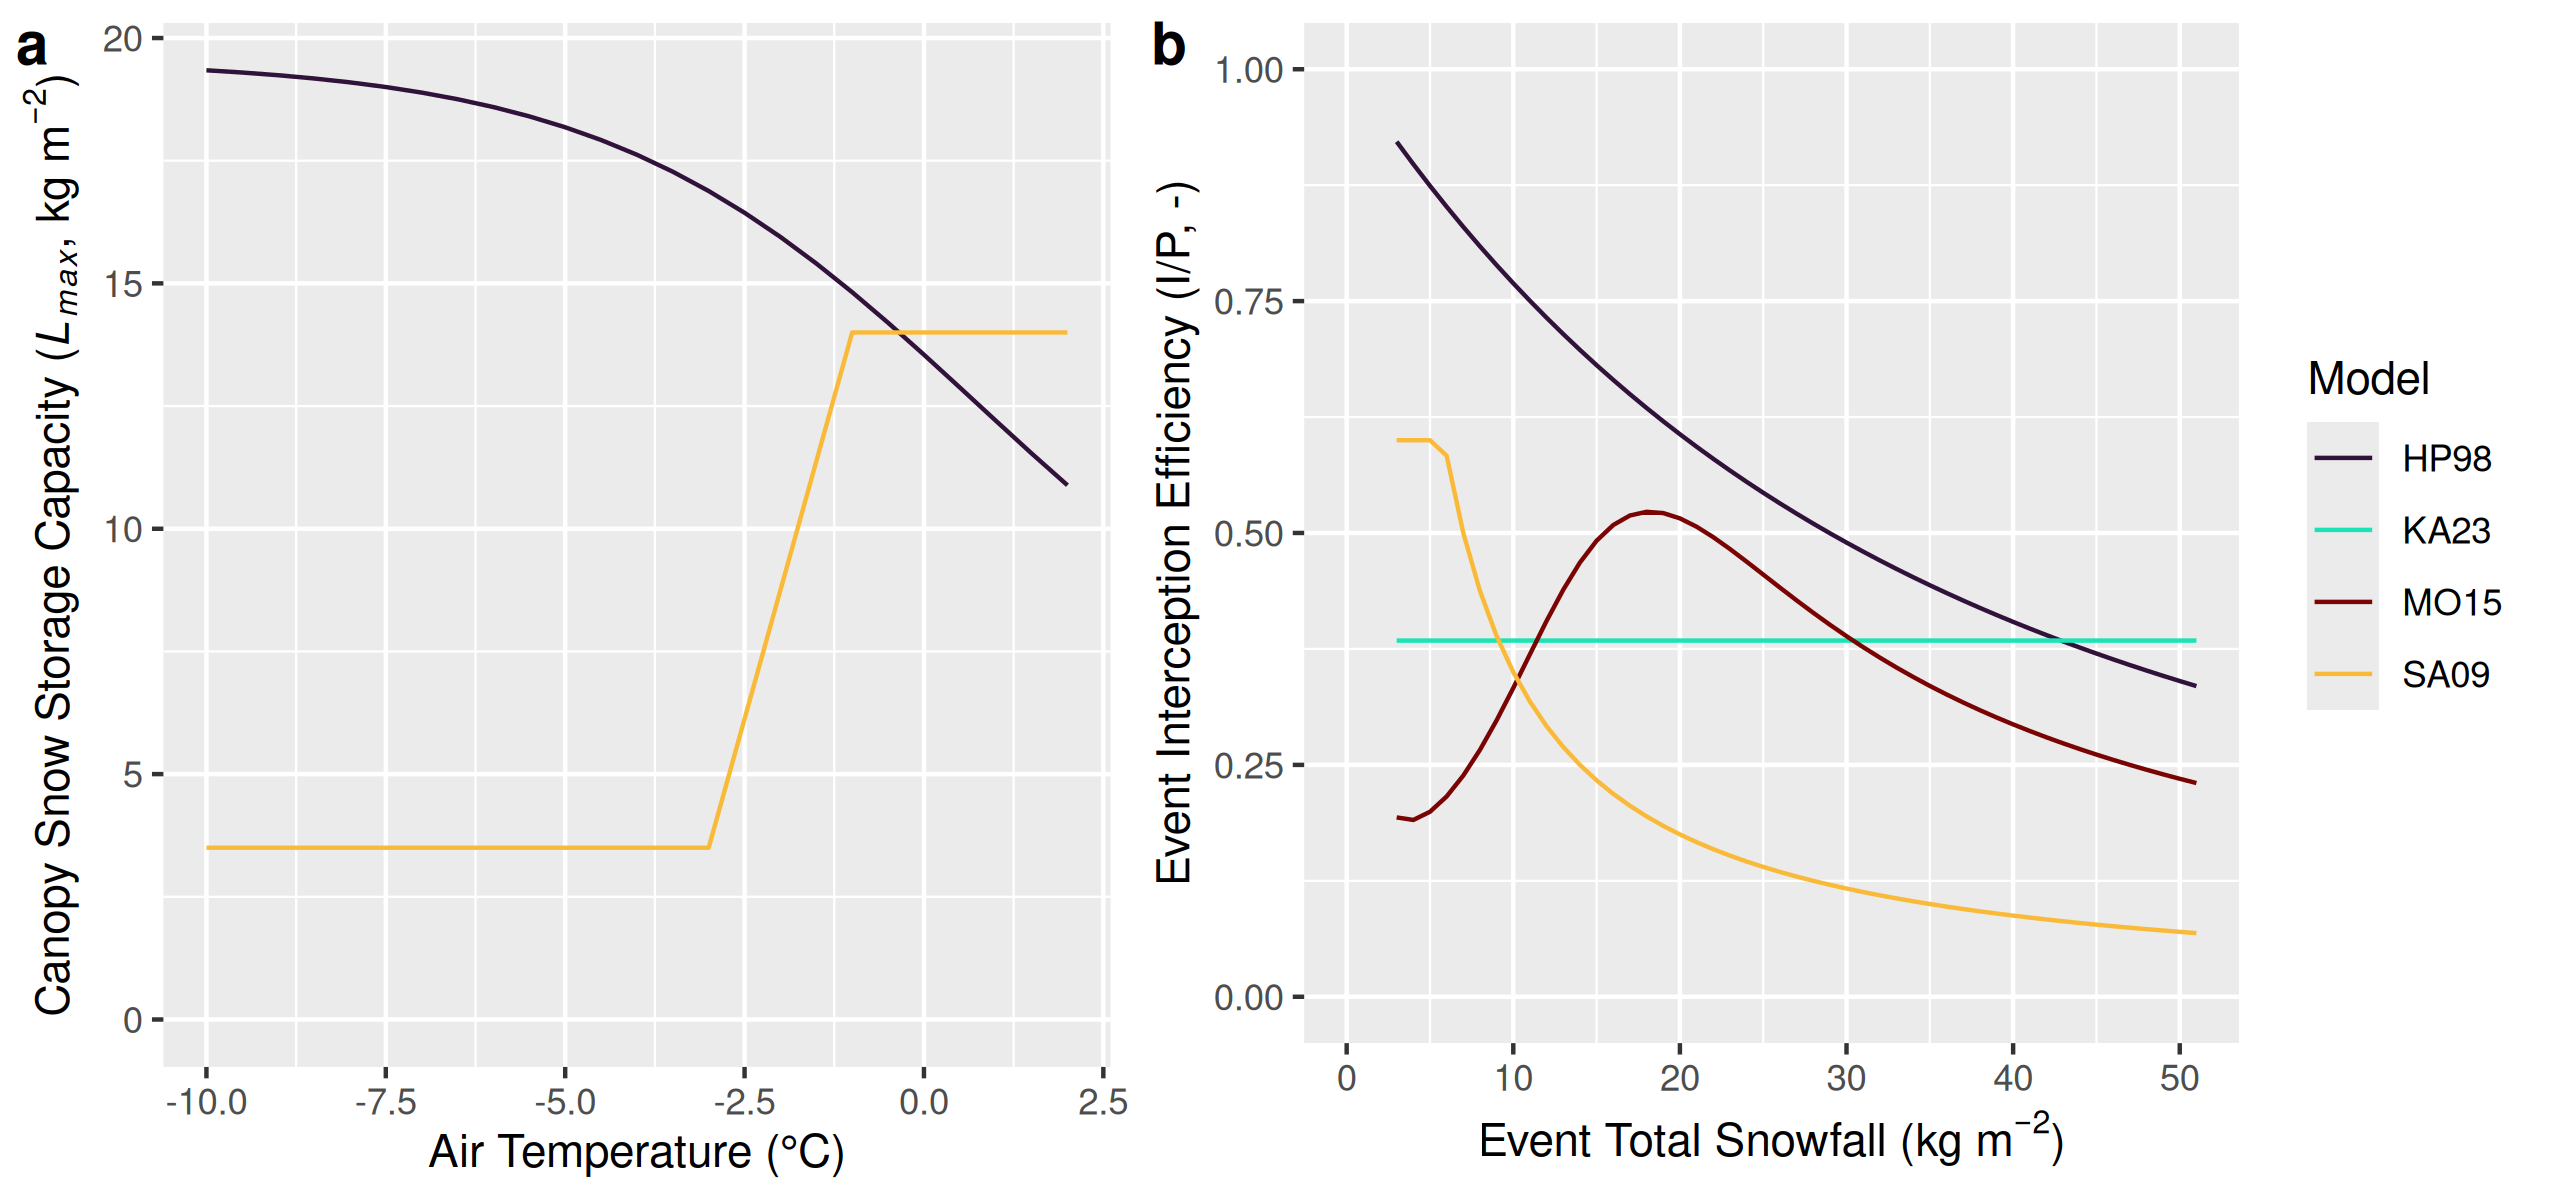
\includegraphics[keepaspectratio]{chapters/02-review-paper/figs/figure6.png}}

}

\caption{\label{fig-example-wmax-ip}Panel (a) Comparison of the Hedstrom
\& Pomeroy (1998) (HP98) and Andreadis et al. (2009) (SA09) canopy snow
storage capacity parameterisations. Panel (b) shows interception
efficiency for event totals as the change in event canopy snow load
divided by the corresponding change in event snowfall in the open for
parameterisations: HP98, Katsushima et al., (2023) (KA23), SA09, and
Moeser et al., (2009) (M15). Initial canopy load is held at 0, air
temperature is -5°C, LAI of 3.5 and the HP98 species coefficient for
spruce (5.9 kg m\textsuperscript{-2}).}

\end{figure}%

\begin{figure}

\centering{

\pandocbounded{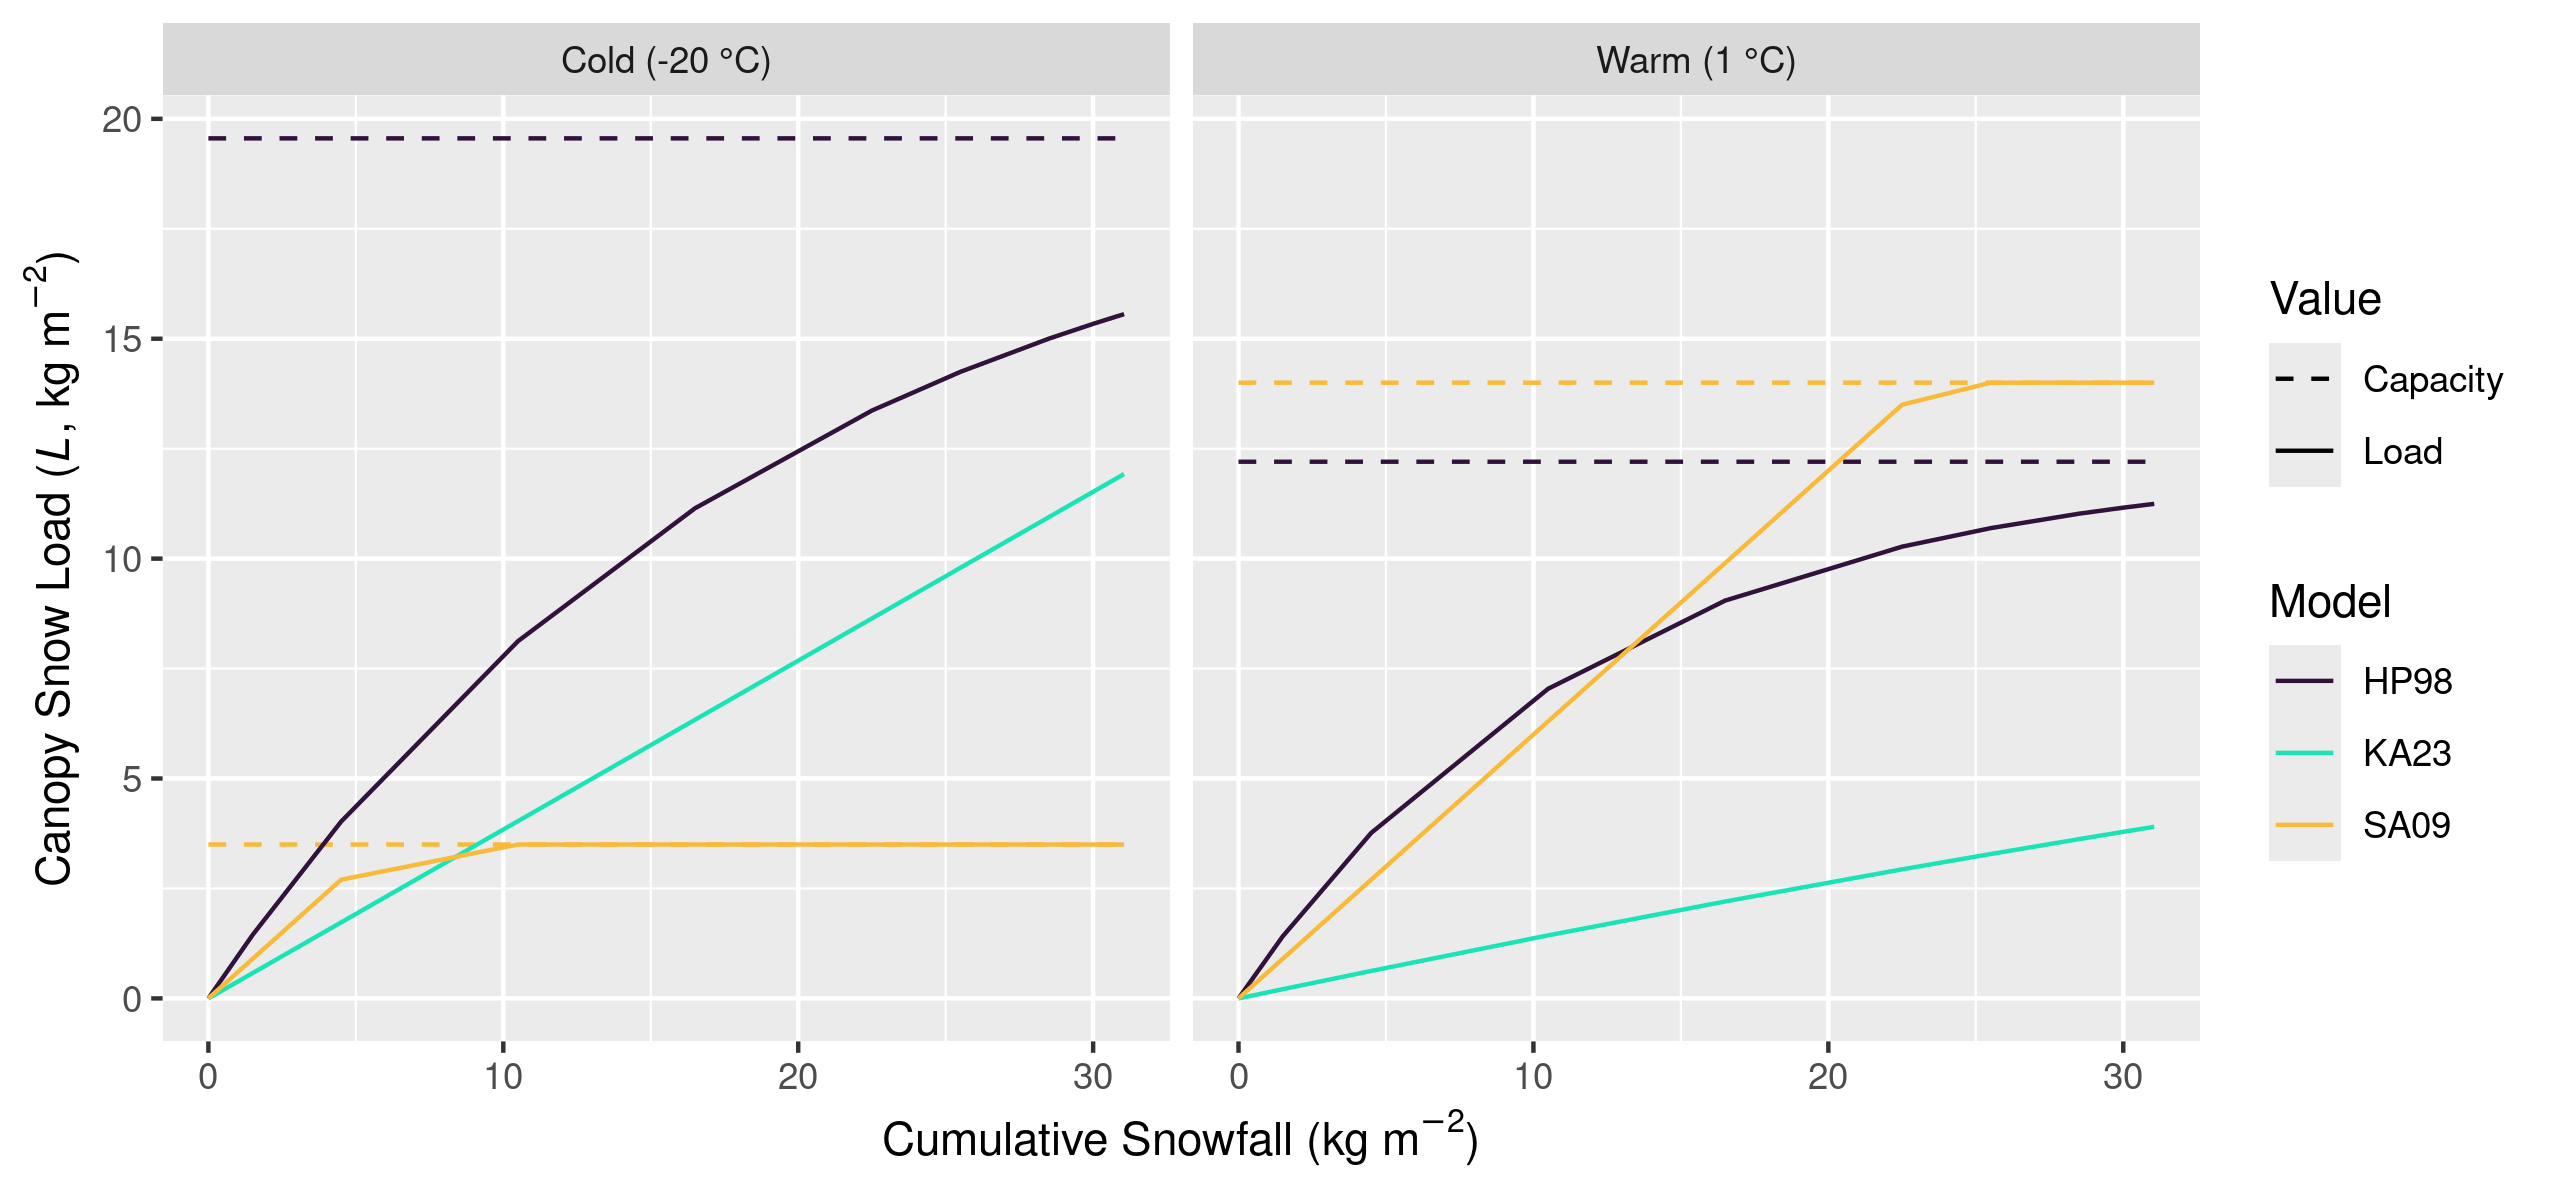
\includegraphics[keepaspectratio]{chapters/02-review-paper/figs/figure7.png}}

}

\caption{\label{fig-L-cold-warm}The state of canopy snow load (solid
lines) for a cold and warm event using the parameterisations by Hedstrom
and Pomeroy (1998) (HP98), Katsushima et al., (2023), combined Storck et
al.~(2002) and Andreadis et al., (2009) (SA09). The interception storage
capacity is shown for the HP98 (purple) and SA09 (orange)
parameterisations using a horizontal dashed line. The KA23
parameterisation does not include a canopy snow storage capacity. To
isolate the influence of snow interception parameterisations ablative
processes have not been computed. Constants for these two plots include
a wind speed of 1 m s\textsuperscript{-1}, LAI of 3.5 (-) and the HP98
species coefficient for spruce (5.9 kg m\textsuperscript{-2}).}

\end{figure}%

\begin{longtable}[]{@{}
  >{\raggedright\arraybackslash}p{(\linewidth - 6\tabcolsep) * \real{0.2500}}
  >{\raggedright\arraybackslash}p{(\linewidth - 6\tabcolsep) * \real{0.2500}}
  >{\raggedright\arraybackslash}p{(\linewidth - 6\tabcolsep) * \real{0.2500}}
  >{\raggedright\arraybackslash}p{(\linewidth - 6\tabcolsep) * \real{0.2500}}@{}}
\caption{Summary of canopy interception/precipitation (I/P) model
behaviour and measurement
techniques.}\label{tbl-mod-desc}\tabularnewline
\toprule\noalign{}
\begin{minipage}[b]{\linewidth}\raggedright
Model
\end{minipage} & \begin{minipage}[b]{\linewidth}\raggedright
Variables
\end{minipage} & \begin{minipage}[b]{\linewidth}\raggedright
General Description
\end{minipage} & \begin{minipage}[b]{\linewidth}\raggedright
Measurement Technique
\end{minipage} \\
\midrule\noalign{}
\endfirsthead
\toprule\noalign{}
\begin{minipage}[b]{\linewidth}\raggedright
Model
\end{minipage} & \begin{minipage}[b]{\linewidth}\raggedright
Variables
\end{minipage} & \begin{minipage}[b]{\linewidth}\raggedright
General Description
\end{minipage} & \begin{minipage}[b]{\linewidth}\raggedright
Measurement Technique
\end{minipage} \\
\midrule\noalign{}
\endhead
\bottomrule\noalign{}
\endlastfoot
Satterlund \& Haupt (1967) & \(L_{max}\), \(K\), \(q_{sf}\),
\(P_{sf}^{e}\) & I/P initially rises due to rising \(L\) which bridges
gaps and increases \(C_p\). I/P later declines when \(L\) approaches
\(L_{max}\) due to branch bending which reduces \(C_{p}\) and increases
unloading. & Weighed tree lysimeter \\
Hedstrom \& Pomeroy (1998) & \(C_{p}(C_{c},u,w,H,J)\), \(L\), \(L_{0}\),
\(q_{sf}\), \(L_{max}(S,\overline{S},LAI,ρ_{s},T_{a})\) & I/P starts
high and then declines as \(L\) approaches \(L_{max}\) which reduces
\(C_{p}\) and increases unloading. This decline is stronger for warmer
\(T_{a}\) as branches bend more easily. & Snow survey mass balance \\
Storck et al.~(2002) & \(L_{max}(L_{r},T_{a},m,LAI)\) & I/P is constant
over time and space. \(L_{max}\) increases with \(LAI\) and increases as
a step function of \(T_a\) due to higher cohesion and adhesion. When
\(L > L_{max}\) new snow is unloaded to the surface snowpack. & Weighed
tree lysimeter with subcanopy lysimeter \\
Roth \& Nolin (2019) & \(q_{sf},T_{a},G_{z}\) & I/P increases with
increasing \(T_{a}\) and a lidar derived canopy structure metric
\(G_{z}\). & Paired open and forested acoustic snow depth sensors and
aerial lidar canopy metrics \\
Katsushima et al.~(2023) & \(L,T_{a},u_{1/3}\) & I/P decreases with
increasing \(u_{13}\) when \(T_{a}\) \textless{} 0°C, I/P increases with
\(T_{a}\) when \(-4^{\circ}C \le T_{a} < 0^{\circ}C\), and I/P decreases
with \(T_{a}\) and \(L\) when \(T_{a}\) \textgreater{} 0°C. & Weighed
tree lysimeter \\
\end{longtable}

\subsubsection{Hedstrom \& Pomeroy (1998)}\label{hedstrom1998}

In the observations collected by Hedstrom \& Pomeroy (1998) in the
southern boreal forest from a Jack Pine and Black Spruce stand, snow
interception efficiency starts high and then declines and was
represented using an inverse exponential function
(Figure~\ref{fig-example-wmax-ip}, b). Hedstrom \& Pomeroy (1998)
describe a relationship to relate \(q_{tf}(L)\) to interception
efficiency, \(\frac{I}{P}(L)\), the fraction of snow intercepted over a
snowfall period, both of which are proposed to be a function of \(L\).
The mass balance method (i.e., Equation~\ref{eq-dwdt-ode}) was used to
estimate \(\frac{I}{P}\) which incorporated fresh snow survey
measurements of \(\Delta_{tf}\) at the plot scale and \(\Delta_{sf}\) to
an open clearing over events with \(\Delta t\) ranging from days to
weeks. Average cumulative snowfall over these events was 4 kg
m\textsuperscript{-2} with event temperatures ranging from -40 °C to
near 0 °C and very low wind speeds (exact values not reported). These
measurements, in addition to those collected by Schmidt \& Gluns (1991)
were used to formulate the Hedstrom \& Pomeroy (1998) snow interception
parameterisation. Hedstrom \& Pomeroy (1998) calculate \(q_{tf}\) as:

\begin{equation}\phantomsection\label{eq-tf-ode}{
q_{tf}(L) = \begin{cases}
    \left(1-\frac{I}{P}(L)\right)q_{sf},& \text{if } L< L_{max}\\
    q_{sf},              & \text{otherwise}
\end{cases}
}\end{equation}

\(\frac{I}{P}(L)\) is calculated as:

\begin{equation}\phantomsection\label{eq-ip}{
\frac{I}{P}(L) = \frac{\Delta L}{\overline{q_{sf}} \Delta t} 
}\end{equation}

where \(\overline{q_{sf}}\) (kg m\textsuperscript{-2}), is the average
snowfall rate over the discrete time interval \(\Delta t\). For a given
snowfall event, Hedstrom \& Pomeroy (1998) propose a function to
calculate \(\frac{I}{P}(L)\) as:

\begin{equation}\phantomsection\label{eq-hp98-int-smpl1}{
\frac{I}{P}(L) = C_{p}\frac{L_{max}-L}{L_{max}}
}\end{equation}

where \(C_{p}\) (-) is the fraction of snow-leaf contact area per unit
area of ground. Equation~\ref{eq-hp98-int-smpl1} has been simplified
slightly from the original formula presented in Hedstrom \& Pomeroy
(1998). See Equation~\ref{eq-hp98-int-orig} in
Section~\ref{sec-review-appendix} for the steps to simplify.

The calculation of \(C_{p}\) in Hedstrom \& Pomeroy (1998) is:

\begin{equation}\phantomsection\label{eq-hp98-cp}{
C_{lca} = \frac{C_c}{1-\frac{C_cuH}{wJ}}
}\end{equation}

where \(C_c\) (-) is the canopy closure, \(u\) (m s\textsuperscript{-1})
is the horizontal velocity of the snow particle (approximated by wind
speed), \(w\) (m s\textsuperscript{-1}) is the snow particle vertical
fall velocity, \(H\) (m) is the height of the canopy, \(J\) (m) is the
forested downwind distance. Since \(w\) is not a commonly available
meteorological forcing variable Hedstrom \& Pomeroy (1998) assume a
constant of 0.8 m s\textsuperscript{-1}. In the absence of detailed
canopy structure metrics \(J\) is difficult to determine in practice. An
example of how \(C_p\) varies with wind speed and canopy coverage is
shown in Figure~\ref{fig-example-lca}. A limit in the increase in
\(C_p\) is shown in Figure~\ref{fig-example-lca} as \(C_p\) reaches 1.0
and does not increase further at a wind speed of 2 m
s\textsuperscript{-1} and \(C_c\) of 0.8.

\begin{figure}

\centering{

\pandocbounded{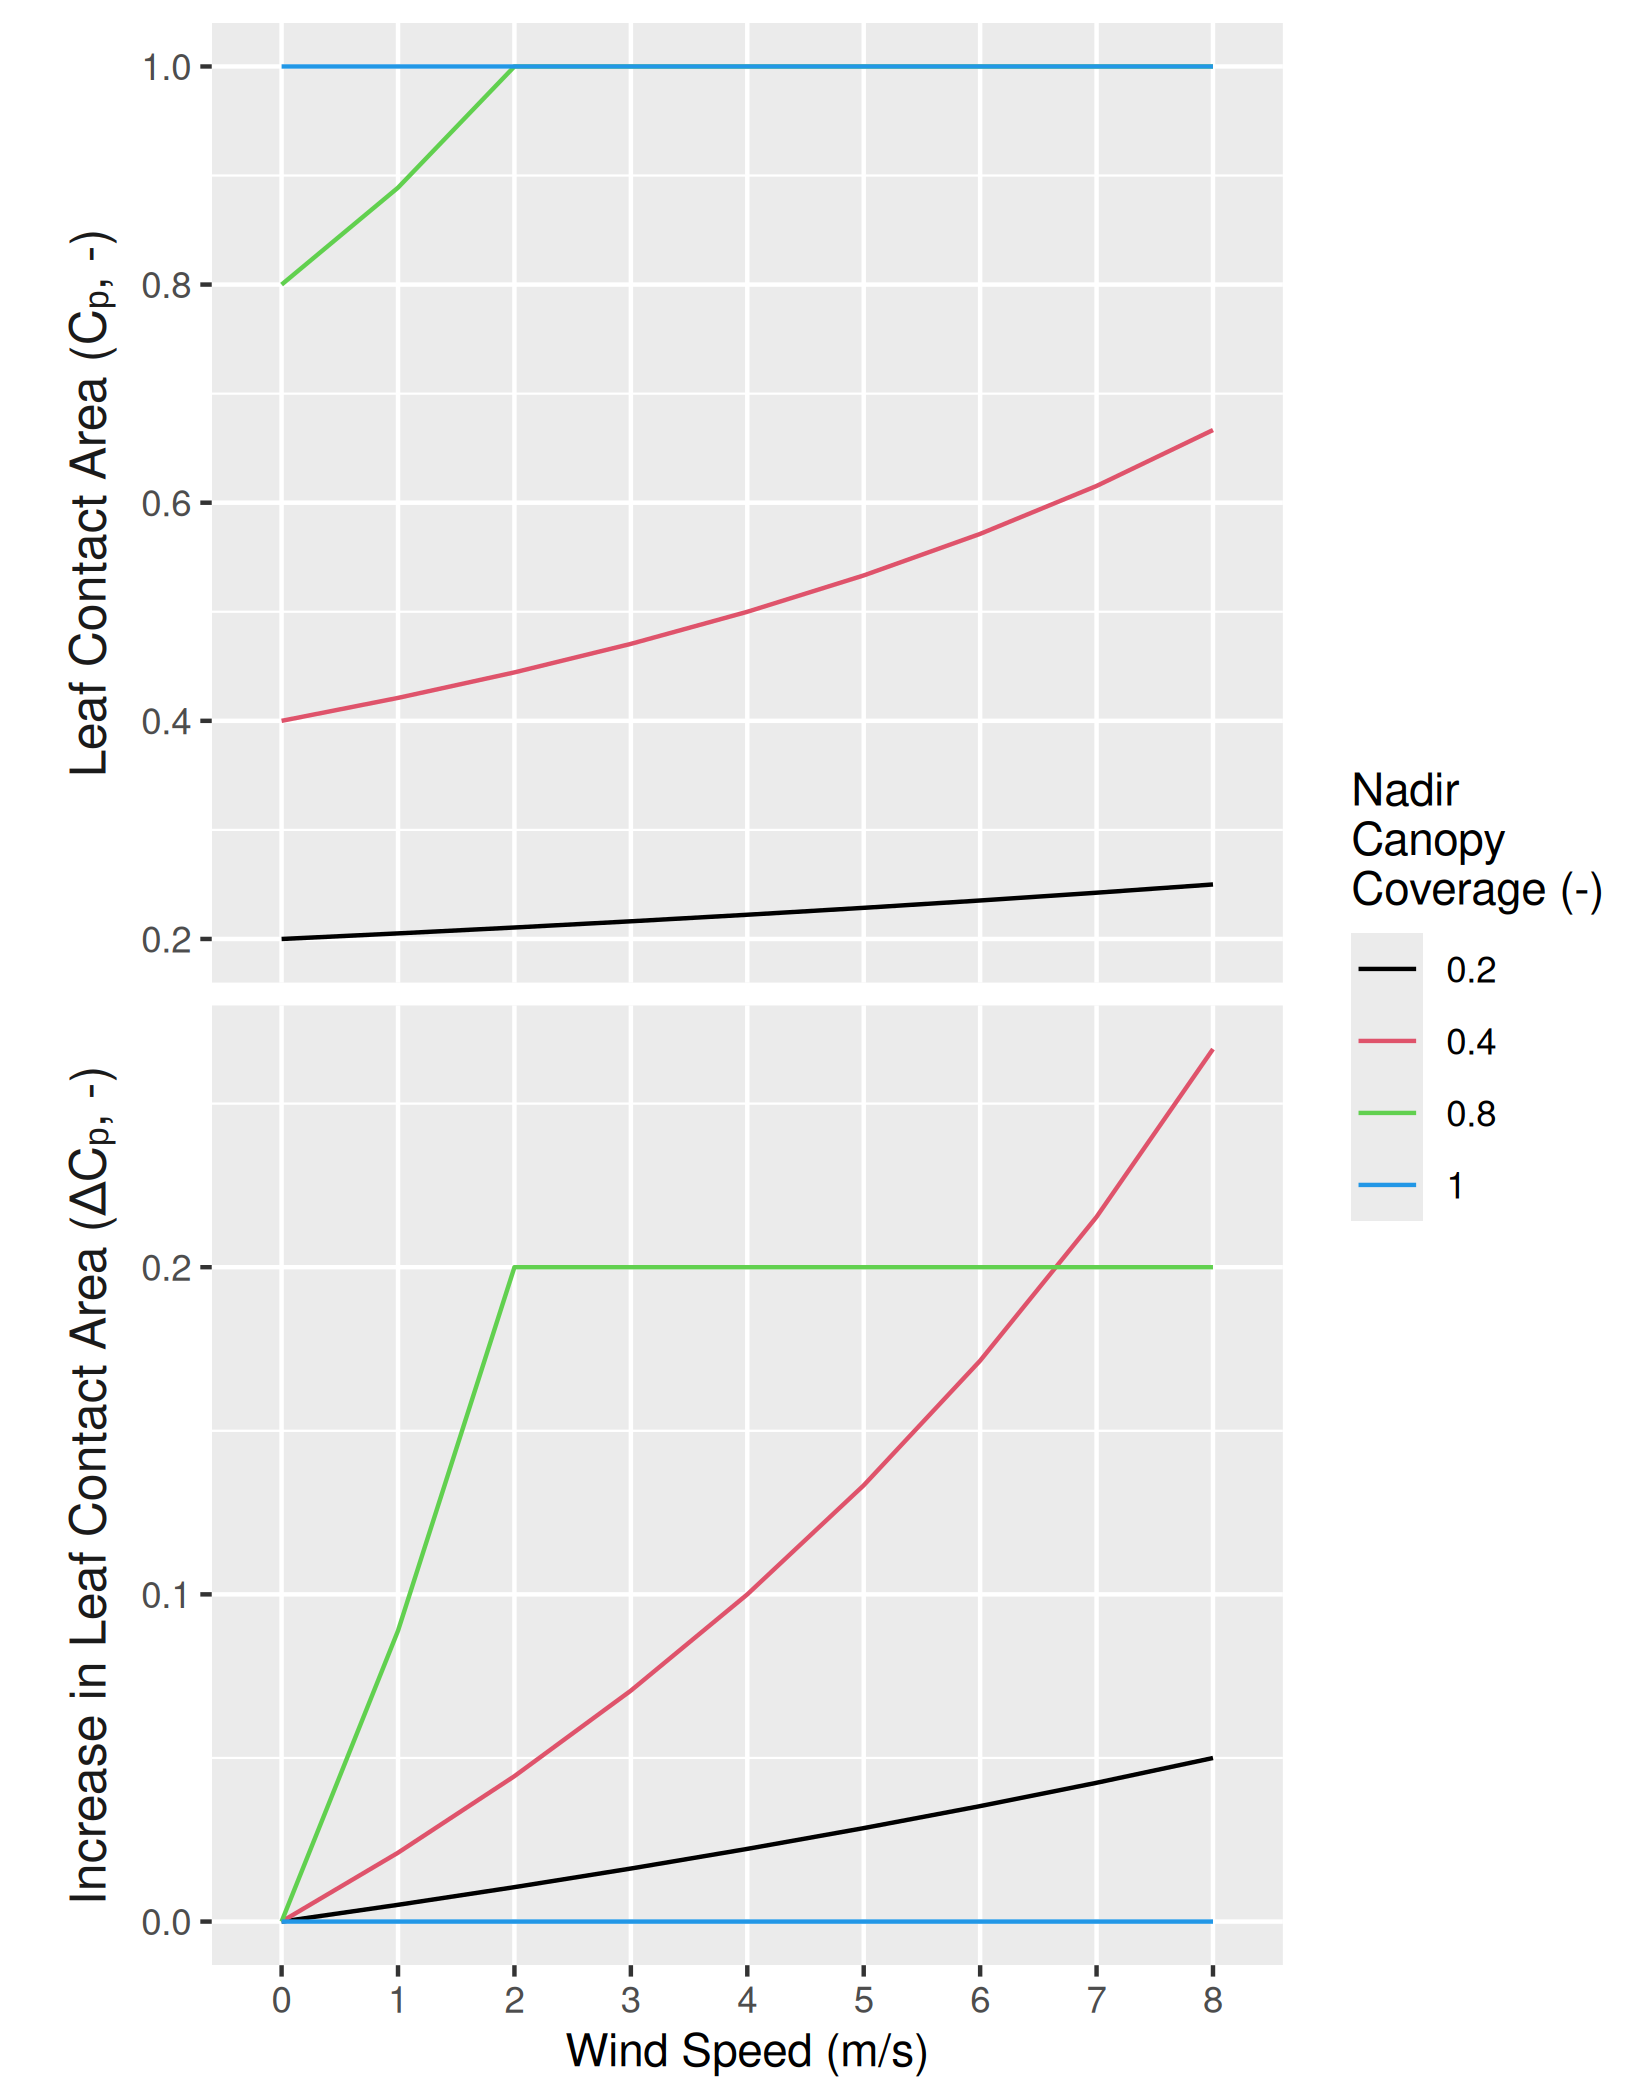
\includegraphics[keepaspectratio]{chapters/02-review-paper/figs/figure8.png}}

}

\caption{\label{fig-example-lca}Plots showing the leaf contact area
(top) and increase in leaf contact area (bottom) with increasing wind
speed calculated using the method from Hedstrom \& Pomeroy (1998). The
colour of each line represents the leaf contact area at nadir which is
equal to the canopy coverage. Here the canopy height is held constant at
10 m, the forested downwind distance is 100 m, and the fall velocity is
0.8 m s\textsuperscript{-1}.}

\end{figure}%

Hedstrom \& Pomeroy (1998) integrate Equation~\ref{eq-hp98-int-orig} to
provide an analytical solution to calculate the change in intercepted
snow load, \(\Delta L\) (kg m\textsuperscript{-2}) over a discrete time
interval:

\begin{equation}\phantomsection\label{eq-hp98-int-numeric}{
\Delta L = (L_{max}-L_0)\left(1- \text{exp} \left(-\frac{C_{lca}}{L_{max}} \overline{q_{sf}} \Delta t \right) \right)
}\end{equation}

where \(L_0\) (kg m\textsuperscript{-2}) is the canopy snow load before
snowfall is added to the canopy and \(L_{max}\) (kg
m\textsuperscript{-2}) is the canopy snow storage capacity. The steps of
the derivation of Equation~\ref{eq-hp98-int-numeric} from
Equation~\ref{eq-hp98-int-smpl1} are shown in
Equation~\ref{eq-interception-integration-steps} of
Section~\ref{sec-review-appendix}. Equation~\ref{eq-hp98-int-numeric}
has similar form to the rainfall interception parameterisations
developed by (Aston, 1979; Merriam, 1960):

\begin{equation}\phantomsection\label{eq-merriam-int}{
\Delta L = (L_{max})\left(1- \text{exp} \left(- \gamma \overline{q_{sf}} \Delta t \right) \right)
}\end{equation}

with \(\gamma\) being an exponential fitting parameter.

Hedstrom \& Pomeroy (1998) calculate \(L_{max}\) as:

\begin{equation}\phantomsection\label{eq-l-max}{
L_{max} = S \cdot LAI
}\end{equation}

where \(LAI\) (dimensionless) is the leaf area index, and \(S\) (kg
m\textsuperscript{-2}) is a species maximum snow load correction factor
that is a function of snow density:

\begin{equation}\phantomsection\label{eq-species-correction}{
S = \overline{S} (0.27 + \frac{46}{\rho_s})
}\end{equation}

where \(\rho_s\) (kg m\textsuperscript{-3}) is the fresh snow density
(kg m\textsuperscript{-3}) and Schmidt \& Gluns (1991) observed
\(\overline{S}\) = 6.6 and 5.9 kg m\textsuperscript{-2} for pine and
spruce, respectively.

Fresh snow density \(\rho_s\) was estimated by Hedstrom \& Pomeroy
(1998) based on a regression through observations from sites in
Saskatchewan and Yukon (Hedstrom \& Pomeroy, 1998), the Fraser
Experimental Forest, Colorado (1989) and Nelson, British Columbia (1990)
(Schmidt \& Gluns, 1991), and the Central Sierra Snow Laboratory,
California (of Engineers, 1956) as:

\begin{equation}\phantomsection\label{eq-rhoSnow}{
\rho_s = 67.92 + 51.25 e ^{(T_{a})/2.59}
}\end{equation}

where \(T_a\) is the ambient air temperature (°C). According to this
equation, \(\rho_s\) increases with higher temperatures which will
result in lower \(S\) and subsequently lower \(L_{max}\)
(Figure~\ref{fig-example-wmax-ip}, a), resulting in the lower canopy
snow loads for warm temperatures compared to cold temperatures shown in
Figure~\ref{fig-L-cold-warm}). There are other factors not directly
accounted for by this equation such as solar radiation, humidity,
hydrometeor type and size, wind speed, and compression of snow which may
contribute to the melt and/or metamorphism of fresh snowfall.

\subsubsection{Storck et al. (2002) and Andreadis et al.
(2009)}\label{storck2002-and-andreadis2009}

Andreadis et al. (2009) developed a snow interception parameterisation
using data collected by Storck et al. (2002) in dense old growth forest
in the maritime climate of southwestern Oregon, USA. Storck et al.
(2002) used a weighed tree lysimeter (Douglas fir, Ponderosa pine, White
fir, and Lodgepole pine) to measure \(\frac{dL}{dt}\), a subcanopy
lysimeter (installed beneath the subcanopy snowpack) measured
\(q_{tf}+q_{unld}+q_{drip}+q_{discharge}\), and \(q_{sf}\) was measured
in an open clearing. Using these point scale measurements Storck et al.
(2002) attempted to isolate the individual processes in
Equation~\ref{eq-canopy-mass-bal} to develop their process
understanding. The opposing relationship and increased sensitivity of
the Storck et al. (2002) calculation of canopy snow storage capacity to
air temperature compared to Hedstrom \& Pomeroy (1998) is shown in
Figure~\ref{fig-example-wmax-ip}. The observations from Storck et al.
(2002) found \(\frac{I}{P}\) was equal to a constant of 0.6 up to canopy
snow loads of 40 kg m\textsuperscript{-2}. This results in the positive
linear relationship of \(L\) with increasing snowfall until \(L_{max}\)
is reached (Figure~\ref{fig-L-cold-warm}). This is similar to the
observations by Calder (1990) who also observed a constant value of
\(\frac{I}{P}(L)\) for canopy snow loads up to 30 mm in the uplands of
Scotland (see Fig. 2 in Lundberg \& Halldin, 2001). Storck et al. (2002)
limit, \(L\) as being less than or equal to \(L_{max}\) using a step
function of temperature.

Storck et al. (2002) calculate \(L_{max}\) as:

\begin{equation}\phantomsection\label{eq-imax-storck-andreas}{
L_{max} = L_r \cdot m \cdot LAI
}\end{equation}

where \(m\) (kg m\textsuperscript{-2}) is an empirical parameter
determined based on their observations of the canopy snow storage
capacity (default value = \(5 \cdot e^{-6}\)), \(L_r\) (dimensionless)
is a step function of temperature based on observations by Kobayashi
(1987) of snow cohesion on a plank of wood and Pfister \& Schneebeli
(1999) and Storck et al. (2002) who observed that snow interception
decreases with decreasing temperatures. Based on these observations
\(L_r\) is calculated as:

\begin{equation}\phantomsection\label{eq-storck-andreas-lr}{
L_r = \begin{cases}
    4,& \text{if } T_a>-1 ^{\circ} C \\
    1.5 T_a+5.5,              & \text{if } -1 ^{\circ} C \geq T_a >-3 ^{\circ} C \\
        1.0,              & \text{if } T_a \leq -3 ^{\circ} C
\end{cases}
}\end{equation}

The Storck et al. (2002) dataset was derived from observed snowfall
events of 5---80 kg m\textsuperscript{-2} with an average of
\textasciitilde15 kg m\textsuperscript{-2}, winds less than 2 m
s\textsuperscript{-1} and relatively warm air temperatures above -5°C.

\subsubsection{Katsushima et al. (2023)}\label{katsushima2023}

More recent work by Katsushima et al. (2023) collected measurements of
snow interception using a weighed Japanese cedar tree (\emph{Cryptomeria
japonica}) in a warm-humid coastal environment. To isolate periods of
interception without unloading they selected weighed tree observations
at night with precipitation rate \(\ge\) 1 kg m\textsuperscript{-2}
hr\textsuperscript{-1}, wind speed \(\le\) 1 m s\textsuperscript{-1},
and an air temperature of \(\le\) 1.5 °C. Katsushima et al. (2023)
observed a decline in interception efficiency with increasing wind
speed, which they attributed to increased hydrometeor velocity and
bouncing on impact. They did not observe a maximum interception capacity
within their canopy snow load measurement range of 0-25 kg
m\textsuperscript{-2}. Katsushima et al. (2023) propose a new step-based
equation based on their observations in Japan for the calculation of
\(\frac{I}{P}(L, T_a, v)\) as a function of \(L\), wind speed and air
temperature:

\begin{equation}\phantomsection\label{eq-kat-ip}{
\frac{I}{P}(L) = \begin{cases}
    0.73-0.59T_a-0.0082L,& \text{if } T_a\geq 0 ^{\circ} C \\
    0.86+0.064T_a-0.22v_{1/3},              & \text{if } -4 ^{\circ} C \leq T_a <0 ^{\circ} C \\
        0.86+0.064\cdot(-4)-0.22v_{1/3},              & \text{if } T_a < -4 ^{\circ} C
\end{cases}
}\end{equation}

where \(T_a\) is the air temperature (°C) 4 m above the ground and
\(v_{1/3}\) is the wind speed (m s\textsuperscript{-1}) at one-third of
the canopy height.

\subsubsection{Event Based Snow Interception
Parameterisations}\label{event-based-snow-interception-parameterisations}

Additional snow interception parameterisations are available in the
literature that approximate the increase in canopy load over a snowfall
accumulation period. However, since these parameterisations were
developed over events with varying time intervals, they cannot directly
be included in hydrological models that run on regular time intervals.
Still, the work by Satterlund \& Haupt (1967), Moeser et al. (2015b) and
Roth \& Nolin (2019) has been important to develop theory on the
influence of forest structure on snow interception.

Satterlund \& Haupt (1967) derived a snow interception function by
fitting a curve to observations of snow accumulation on a weighing tree
over two storms in Idaho. The two storms had accumulated snowfall
ranging from 0.5---7 kg m\textsuperscript{-2} and temperatures close to
0°C with little wind. These observations showed an initial increase in
the rate of intercepted snow, as snowflakes bridge gaps between needles.
The initial low interception efficiency was followed by an increase and
then flattening off of the interception rate as branches bent due to the
weight of snow which Satterlund \& Haupt (1967) represented by a
numerical analytical sigmoidal function fitted to their observed data:

\begin{equation}\phantomsection\label{eq-satterlund}{
\Delta L = \frac{L_{max}}{1+\text{exp}^{-K(\overline{q_{sf}} \Delta t-P_{sf}^e)}}
}\end{equation}

where \(K\) is a constant expressing the rate of interception (kg
m\textsuperscript{-2} \textsuperscript{-1}), and \(P_{sf}^e\) (kg
m\textsuperscript{-2}), is the amount of snowfall accumulated at the
point of most rapid loading.

The Moeser et al. (2015b) parameterisation is based on the Satterlund \&
Haupt (1967) sigmoidal growth curve, Equation~\ref{eq-satterlund}, and a
modification to the Hedstrom \& Pomeroy (1998) \(L_{max}\) function
(Figure~\ref{fig-example-wmax-ip}, b). Their modifications to
\(L_{max}\) were informed by detailed measurements of canopy structure
derived from aerial LiDAR and manual snow depth measurements within a
dense forest with a temperate climate in Switzerland. The observations
in the Moeser et al. (2015b) study are based on snowfall events of 13 to
27 cm in a temperate climate with observed air temperatures ranging from
-12 °C to -1.9 °C. Since Moeser et al. (2015b) did not observe snowfall
storm events below 10 mm, their decision to use a sigmoidal function
with initially low snow interception efficiency is based observations
from Satterlund \& Haupt (1967).

The Moeser et al. (2015b) formulation of \(L_{max}\) also differs from
the previous studies in that it does not include a parameter for air
temperature. To calculate \(L_{max}\), Moeser et al. (2015b) use the
natural logarithm of mean distance to canopy (\(\overline{D_c}\), m),
and total open area (\(A_o\), m\textsuperscript{2}):

\[
L_{max} = 2.167(\overline{D_c}) + -3.410(\overline{D_c})^2 + 
\]

\begin{equation}\phantomsection\label{eq-moeser-imax}{
55.761(C_c) + 181.858(C_c)^2 + -2.493(A_o) + 0.499(A_o)^2 + 20.819
}\end{equation}

The use of additional forest structure metrics in the Moeser et al.
(2015b) snow interception equation allows for application to highly
heterogeneous forests, something that LAI-based algorithms such as
Hedstrom \& Pomeroy (1998) were not designed for. While lidar-derived
canopy metrics like those in Equation~\ref{eq-moeser-imax} are
beneficial for capturing plot-scale variability in subcanopy snow
accumulation, these metrics are currently not feasible to obtain for
larger scale hydrological models.

A more recent study by Roth \& Nolin (2019) presents another event-based
snow interception algorithm based on point-scale measurements of snow
depth between paired open and forested sites. The Roth \& Nolin (2019)
study was conducted over 6 years at stations located in Oregon with air
temperatures ranging from -14 to 6 °C. The wind speed observed over
their study period is not provided. They make use of a new forest
structure metric, median gap length \(G_z\) which can be derived by
aerial LiDAR observations. Like Andreadis et al. (2009), the Roth \&
Nolin (2019) formulation includes air temperature but rather than using
a step function they use a continuous representation. This new algorithm
is derived using a power law relationship, based on an empirical
relationship with event size, temperature, and forest structure, which
deviates from the exponential function used in Hedstrom \& Pomeroy
(1998) or Moeser et al. (2015b). The Roth \& Nolin (2019) algorithm does
not include a maximum canopy snow capacity, such as used in Hedstrom \&
Pomeroy (1998) and Moeser et al. (2015b), but rather calculates the
change in canopy snow load, \(\Delta L\) (kg m\textsuperscript{-2}) as:

\begin{equation}\phantomsection\label{eq-roth-i}{
\Delta L = \overline{q_{sf}} \Delta t ^{0.04 \cdot T_{air} - 0.75 \cdot G_z + 1.56}
}\end{equation}

where \(\overline{q_{sf}}\) is the average event snowfall rate (kg
m\textsuperscript{-2}), \(T_{a}\) is the within canopy air temperature
(°C), and \(G_z\) is the median gap length versus change in height
(dimensionless).

\subsection{Canopy Snow Ablation Parameterisations}\label{sec-ablation}

Current canopy snow ablation parameterisations are based on measurements
collected in Saskatchewan (Hedstrom \& Pomeroy, 1998), British Columbia
(Floyd, 2012; Schmidt \& Gluns, 1991), Oregon (Storck et al., 2002),
Colorado (Sexstone et al., 2018), Japan (Katsushima et al., 2023;
Yamazaki et al., 1996), and Russia (Gelfan et al., 2004). The following
section will discuss the various processes that ablate snow intercepted
in the canopy.

\subsubsection{Sublimation}\label{sublimation}

To estimate canopy snow sublimation, Pomeroy et al. (1998b) builds on
earlier laboratory experiments by Thorpe \& Mason (1966), applied to
blowing snow by Schmidt (1972) and modified for forested environments by
Schmidt \& Gluns (1991), Pomeroy \& Schmidt (1993), and Pomeroy et al.
(1998b). Since snow intercepted in the canopy is not as well exposed to
the atmosphere as a single ice sphere, Pomeroy \& Schmidt (1993) derived
an exposure coefficient to reduce the rate of sublimation allowing the
calculation to be scaled from particle to the canopy scale. The
sublimation rate for snow in the canopy, \(q_{sub}^{veg}(L)\) (kg
m\textsuperscript{-2} s\textsuperscript{-1}) can be calculated as:

\begin{equation}\phantomsection\label{eq-pom98-v_i}{
q_{sub}^{veg}(L) = \kappa_{sub}^{sphere} C_e L
}\end{equation}

where \(C_e\) is a dimensionless exposure coefficient. Methods to
estimate \(C_e\) are described in Pomeroy et al. (1998b).

The sublimation rate coefficient for single ice spheres,
\(\kappa_{sub}^{sphere}\) (s\textsuperscript{-1}), is represented as a
function of the mass \(m\) (kg) of the ice sphere:

\begin{equation}\phantomsection\label{eq-pom98-sublimation}{
\kappa_{sub}^{sphere} = \frac{dm}{m \ dt} = \frac{
  \frac{2 \pi r}{m} (\frac{\rho_{wa}}{{\rho_s}}-1) - K J
}{
  \lambda_{sub} J + \frac{1}{D \rho_s Sh}
}
}\end{equation}

with a radius \(r\) (m) where \(\rho_{wa}\) (kg m\textsuperscript{-3}),
is the water vapour density of the remote environment, \(\rho_s\) (kg
m\textsuperscript{-3}) is the saturation water vapour density at
temperature \(T_a\) (K) for the particle surface, \(D\) is the
diffusivity of water vapour in still air (m\textsuperscript{2}
s\textsuperscript{-1}), \(Sh\) is the Sherwood number indexing the
turbulent transfer of water vapour (-), and \(K\) is the net shortwave
radiation flux (W m\textsuperscript{-2}) to the particle found as:

\begin{equation}\phantomsection\label{eq-pom98-sw}{
K = \pi r^2 (1-\alpha) S \downarrow
}\end{equation}

where \(\alpha\) (dimensionless) is the particle shortwave albedo and
\(S \downarrow\) (W m\textsuperscript{-2}) is the incoming shortwave
radiation.

\(J\) is found as:

\begin{equation}\phantomsection\label{eq-pom98-j}{
J = \frac{1}{\lambda_T T_a Nu} \left[ \frac{\lambda_{sub} M}{R T_a} -1 \right]
}\end{equation}

where \(R\) is the universal gas constant (8313 J
kmole\textsuperscript{-1} K\textsuperscript{-1}), \(M\) (kg
kmole\textsuperscript{-1}) is the molecular weight of water,
\(\lambda_T\) is the thermal conductivity of the atmosphere (W
m\textsuperscript{-1} K\textsuperscript{-1}), and \(Nu\) is the Nusselt
number (-). Values of acceptable constants and coefficients for the
above equations are given in Pomeroy \& Gray (1995).

\subsubsection{Unloading and Drip}\label{sec-unloading}

Hedstrom \& Pomeroy (1998) did not find any association between canopy
snow unloading and meteorological factors such as wind speed and air
temperature in the cold dense canopy of the Saskatchewan boreal forest.
As a result, the rate of canopy snow unloading, \(q_{unld}(L)\),
attributed to snow metamorphism and wind gusts is represented in
Hedstrom \& Pomeroy (1998) as a function of time and \(L\):

\begin{equation}\phantomsection\label{eq-hp98-flu}{
q_{unld}(L) = \kappa_{unld} L
}\end{equation}

where \(\kappa_{unld}\) (s\textsuperscript{-1}), is a time constant.

Integrating Equation~\ref{eq-hp98-flu} provides an analytical solution
for \(L^{t+\Delta t}\), the canopy snow load following unloading over a
discrete time interval, \(\Delta t\) (s\textsuperscript{-1}):

\begin{equation}\phantomsection\label{eq-hp98-exp-decay}{
L^{t+\Delta t} =L^t\  \text{exp} ^{-\kappa_{unld}\Delta t}
}\end{equation}

The steps to derive to Equation~\ref{eq-hp98-exp-decay} from
Equation~\ref{eq-hp98-flu} are shown in
Section~\ref{sec-review-appendix}.

Later modifications to the Hedstrom \& Pomeroy (1998) algorithm were
provided in Gelfan et al. (2004) who found that all snow was unloaded
from the canopy as liquid meltwater (drip) within 6 hours when ice-bulb
temperatures remained above freezing for 3 hours with observed wind
speed greater than 0.5 m s\textsuperscript{-1}. Using this concept,
Ellis et al. (2010) built on additional observations by Floyd (2012) to
modify the value of \(\kappa_{unld}\) based on ice-bulb temperature
thresholds to unload canopy snow as either wet clumps (\(q_{unld}\)) or
meltwater drip (\(q_{drip}\)). When the ice-bulb temperature exceeds the
snow threshold, snow is unloaded as \(q_{unld}\); if it exceeds the drip
threshold, all canopy snow is unloaded as \(q_{drip}\) within 6 hours.
The threshold values from Floyd (2012) were found to be 2°C and 4°C for
wet snow and drip unloading respectively.

Storck et al. (2002) found unloading to occur in maritime environments
when air temperature rose above 0°C. The amount of solid snow unloading
from the canopy was found to be linearly proportional to the amount of
meltwater drip from canopy snow. For their field experiment in Oregon,
Storck et al. (2002) provide a ratio of mass release to meltwater drip
found during a two-week snowfall event. During this unloading event they
measured 33 kg m\textsuperscript{-2} to have reached the ground as snow
and 84 kg m\textsuperscript{-2} as meltwater drip resulting in a mass
release to meltwater drip ratio of 0.4. Storck et al. (2002) suggested
wind speed may influence canopy snow unloading; however, this was not
observed due to the low wind speeds observed during their study. Using
the observations from Storck et al. (2002), Andreadis et al. (2009)
created a parameterisation to calculate unloading proportional to the
rate of meltwater drip leaving the canopy \(q_{drip}(L)\).

\begin{equation}\phantomsection\label{eq-sa-unload-dudt}{
q_{unld}(L) = \begin{cases}
    0,& \text{if } L \le L_{res} \\
    X_u q_{drip},              & \text{if }  L > L_{res}
\end{cases}
}\end{equation}

where \(L_{res}\) (kg m\textsuperscript{-2}) is the residual intercepted
snow that can only be melted or sublimated (taken as 5 kg
m\textsuperscript{-2} based on observations from Storck et al. (2002)),
\(X_u\) (-) is the ratio of mass release to meltwater drip (taken as 0.4
from Storck et al., 2002). In Andreadis et al. (2009), \(q_{drip}(L)\)
is calculated by solving an energy balance equation to produce meltwater
drip if sufficient energy is available.

Roesch et al. (2001) proposed a third approach to address unloading and
drip, where the mass release of canopy snow is proportional to a
temperature function, \(f(T)\) (s\textsuperscript{-1}) and a
wind-induced unloading function, \(f(u)\) (s\textsuperscript{-1}):

\begin{equation}\phantomsection\label{eq-roesch-unload}{
q_{unld}(L) = L \cdot [f(T) + f(u)]
}\end{equation}

The theory behind the Roesch et al. (2001) parameterisation is based on
the Yamazaki et al. (1996) study who found an exponential decrease of
interception efficiency with time, temperature and wind speed, with a
response time of 0.5 day when temperature is below 0°C and 1--5 h with a
temperature above 0°C. The Roesch et al. (2001) parameterisation was
also informed by the Miller (1962) study that observed a decline in snow
interception with wind speed greater than 2 m s\textsuperscript{-1}.
Roesch et al. (2001) show that boreal forest observations by Betts \&
Ball (1997), who noted a weak relationship (no R\textsuperscript{2}
given) between low wind speeds (\textless{} 3 m s\textsuperscript{-1})
and occurrence of high above-canopy albedos, also supported their
theory, though no such association was observed in the same environment
by Pomeroy \& Dion (1996) who carefully cleaned their upward facing
radiometers after snowstorms. The outcome of this wind speed denominator
is that 50\% of intercepted snow is unloaded within 6 hours for a wind
speed of 5 m s\textsuperscript{-1}. The Roesch et al. (2001) temperature
induced unloading function, \(f(T)\) (s\textsuperscript{-1}), is:

\begin{equation}\phantomsection\label{eq-roesch-unload-t}{
f(T) = \begin{cases}
    0,& \text{if } T_c < T_m \\
    \frac{T_c - T_m}{C_1},              & \text{if }  T_c \ge T_m
\end{cases}
}\end{equation}

\(T_c\) is the air temperature of the canopy (K), \(T_m\) is a user
defined threshold temperature (270.15 K is suggested by Roesch et al.,
2001) and \(C_1\) is a constant of 1.87 x \(10^5\) (K
s\textsuperscript{-1}). The result of Equation~\ref{eq-roesch-unload-t}
is that once \(T_c\) reaches \(T_m\) canopy snow is unloaded at a rate
proportional to \(T_c\). The Roesch et al. (2001) wind induced unloading
function, \(f(v)\) (s\textsuperscript{-1}), is:

\begin{equation}\phantomsection\label{eq-roesch-unload-v}{
f(u) = \begin{cases}
    0,& \text{if } u_{top} < u_m \\
    \frac{u_{top}}{C_2},              & \text{if }  u_{top} \ge u_m
\end{cases}
}\end{equation}

where \(u_{top}\) (m s\textsuperscript{-1}) is the wind speed at a
height above ground corresponding to the mean canopy height, \(u_m\) is
a threshold wind speed (m s\textsuperscript{-1}) and \(C_2\) is a
constant of 1.56 x \(10^5\) m.

Another approach to estimate \(f(u)\) is provided by Bartlett \&
Verseghy (2015):

\begin{equation}\phantomsection\label{eq-bartlett-unload-v}{
f(u) = 0.38u_{top} -0.13
}\end{equation}

where \(u_{top}\) is the wind speed at the canopy top (m
s\textsuperscript{-1}). Bartlett \& Verseghy (2015) also experimented
with calculating \(f(u)\) based on air temperature and solar radiation
in addition to wind speed but found the addition of three meteorological
variables did not provide consistent improvement across all three sites.

The observations by Katsushima et al. (2023) provide additional insights
on canopy snow unloading from a warm and humid region. To isolate
periods of unloading due to melt, Katsushima et al. (2023) filtered
their weighed tree measurements to daytime periods with a canopy snow
load \textgreater{} 5 kg m\textsuperscript{-2}, a wind speed of
\textless{} 1 m s\textsuperscript{-1} and no precipitation. Using these
periods of unloading due to melt, Katsushima et al. (2023) found a
statistically significant relationship between air temperature, solar
radiation and the unloading rate coefficient due to snowmelt, \(f(T)\)
for a range of temperatures from -3.7--3.5 °C. To isolate periods of
unloading due to wind, weighed tree observations were obtained at night
with a canopy snow load \textgreater{} 5 kg m\textsuperscript{-2}, an
air temperature \textless{} 0°C, and no precipitation. Katsushima et al.
(2023) calculated unloading due to snowmelt, \(f(T)\) as:

\begin{equation}\phantomsection\label{eq-kat-fmelt}{
f(T) = 0.039T_a+0.097Q_{sw}+0.0049L
}\end{equation}

and wind-induced unloading, \(f(u)\) as:

\[
f(u) = 0.020u_{1/3}
\]

where \(u_{1/3}\) is the wind speed at one-third the canopy height.

\section{Discussion}\label{discussion}

\subsection{Differences in Snow Interception
Parameterisations}\label{differences-in-snow-interception-parameterisations}

Various theories have been formulated to describe the mechanisms
underlying the loading of snow into and ablation of snow from the
canopy, offering insights for how to describe these processes in
hydrological models. However, the decision of choosing an appropriate
snow interception parameterisation remains uncertain across different
climates and forests. For maritime climates, Storck et al. (2002)
suggest the increase in cohesive forces amongst snow particles and
adhesive forces between snow clumps to the branch leads to a higher
canopy storage capacity during mild air temperatures (-2 to 0.2 °C) as
shown in Figure~\ref{fig-L-cold-warm}. While Storck et al. (2002)
presents the most comprehensive study to measure the individual
processes in Equation~\ref{eq-canopy-mass-bal}, many of the snowfall
events they observed transitioned between snow and rain which presented
difficulties in isolating snow interception from canopy snow ablation
processes and rainfall interception. The small snowfall events (2--5 kg
m\textsuperscript{-2}) observed by Satterlund \& Haupt (1967) at
temperatures close to 0 °C had very low interception efficiencies.
However, it is unclear how much of an influence canopy snowmelt and
unloading attributed to the warm temperatures contributed to the low
interception efficiency observed by Satterlund \& Haupt (1967). Pomeroy
\& Gray (1995), Hedstrom \& Pomeroy (1998) and Schmidt \& Gluns (1991)
observed a slight decline in interception with above zero air
temperatures as frozen branches thaw and bend, thereby reducing the
effective canopy contact area and increasing the angle of repose of snow
intercepted in the canopy (Figure~\ref{fig-L-cold-warm}). These
observations were used to develop an equation for interception
efficiency presented by Hedstrom \& Pomeroy (1998). However, the
duration (days to weeks) between snow surveys conducted by Hedstrom \&
Pomeroy (1998) likely contributed to increased ablation of canopy snow,
potentially reducing interception efficiency at higher canopy snow
loads. For temperatures above 0°C, Katsushima et al. (2023) also found a
decline in interception efficiency above 10 kg m\textsuperscript{-2}
which support the findings by Hedstrom \& Pomeroy (1998), although these
weighed tree measurements are also influenced by ablation and may
explain the very low snow loads predicted by this parameterisation for
warm events in Figure~\ref{fig-L-cold-warm}.

\subsection{Forest Structure and Snow
Interception}\label{forest-structure-and-snow-interception}

Two of the most commonly used snow interception parameterisations,
Hedstrom \& Pomeroy (1998) and Storck et al. (2002), both use LAI as a
primary variable. However, methods for measuring LAI are highly variable
and may (e.g., plant area index) or may not include both leaf and
non-photosynthetic material, both of which can intercept snow.
Additionally, research by López-Moreno \& Latron (2007) and Staines \&
Pomeroy (2023) has shown variability in the zenith angle of the canopy
hemisphere important for snow interception. These findings challenge the
use of broadband LAI or nadir canopy cover metrics currently employed in
snow interception models. Using novel lidar based snow accumulation and
canopy metrics methods, Staines \& Pomeroy (2023) investigated whether
leaf contact area is influenced by canopy snow load. In a closed canopy,
they found that the number of lidar beam contacts with the canopy
increased with canopy snow load as a result of new snow covering small
canopy gaps. However, in partially open canopy, a decrease in canopy
contacts with increased snow load was observed due to branch bending.
These two processes partially compensated for each other, with an
overall increase in canopy contacts with snow load observed by at the
plot scale (Staines \& Pomeroy, 2023).

Snowflake trajectories are frequently non-vertical (e.g., Thériault et
al., 2012), which can also significantly affect the fraction of leaf
contact area per unit of ground (Herwitz \& Slye, 1995; Staines \&
Pomeroy, 2023; Van Stan et al., 2011). Previous research on rainfall
interception by Herwitz \& Slye (1995) and Van Stan et al. (2011) have
shown rainfall trajectory angle to have an important influence on leaf
contact area, which dramatically altered observed throughfall rates at
the forest plot scale. Moreover, Katsushima et al. (2023) found that air
temperature and wind speed were insufficient to describe interception
efficiency and hypothesize that hydrometeor diameter may be a key factor
to consider. Estimates of the hydrometeor trajectory angle can be made
primarily as a function of wind speed (Herwitz \& Slye, 1995) if
assumptions are made about the hydrometeor vertical velocity, which is
less variability than wind speed. Using this theory, Hedstrom \& Pomeroy
(1998) provide a model, shown in Figure~\ref{fig-example-lca}, of
increasing C\_p with wind speed. However, insufficient observations from
wind-driven snowfall have been made to test this theory or
Equation~\ref{eq-hp98-cp}. As a result, Equation~\ref{eq-hp98-cp} is
typically not included in hydrological model application of snow
interception parameterisations. An assessment of the Hedstrom \& Pomeroy
(1998) theory could be facilitated through new aerial lidar measurements
of snow accumulation and forest structure metrics similar to those
described in Staines \& Pomeroy (2023).

\subsection{In Search of a Canopy Snow Storage
Capacity}\label{in-search-of-a-canopy-snow-storage-capacity}

Recent work by Roth \& Nolin (2019), Lundquist et al. (2021), and
Lumbrazo et al. (2022) have observed higher canopy storage capacities
than those observed by Storck et al. (2002) and Hedstrom \& Pomeroy
(1998). This suggests that the sensitivity of interception efficiency to
the state of canopy snow load (Hedstrom \& Pomeroy, 1998) or air
temperature (Storck et al., 2002) may be less than previously thought.
Measurement uncertainty of throughfall, which may have included some
downward ablation of snow intercepted in the canopy and/or melt of
subcanopy snow, may have contributed to an oversensitivity of the theory
developed by Satterlund \& Haupt (1967) and Hedstrom \& Pomeroy (1998)
to branch bending and bridging. As a result of these measurement
uncertainties, parameterisations derived from empirical observations are
unlikely to be truly isolated from other processes which may contribute
to the underestimate of canopy storage capacities. For example, snow
interception parameterisations that include some degree of ablation,
could lead to potential double counting of ablative processes, such as
unloading or drip, when interception parameterisations are combined with
subsequent unloading and drip routines, unless these were calibrated to
include any early ablation (e.g. Hedstrom \& Pomeroy, 1998).

The deposition of water vapour as rime-ice in the forest canopy has also
been shown to accumulate large amounts of snow and ice in the canopy
(Berndt \& Fowler, 1969; Lumbrazo et al., 2022), which are greater than
the Hedstrom \& Pomeroy's (1998) and Storck et al.~(2002)'s canopy
storage capacities and exhibit ablation rates much lower than existing
models (Lumbrazo et al., 2022). For example, observations from Berndt \&
Fowler (1969) found 50 kg m\textsuperscript{-2} of rime-ice accumulated
on the canopy during precipitation free days over a winter season.
Lehtonen et al. (2016) also note the potential for rime-ice accretion to
contribute to forest damage due to heavy canopy loads causing stem
breakage. Under projected future climate in eastern and northern
Finland, Lehtonen et al. (2016) found that heavy snow loads from rime
and wet snow were expected to increase due a more humid and warmer
climate. Aside from the Lehtonen et al. (2016) study in Finland,
rime-ice accumulation is not typically included in snow interception
parameterisations and may contribute to an underestimation of snow loads
in coastal-temperate climates under certain conditions.

\subsection{Differences in Canopy Snow Ablation
Parameterisations}\label{differences-in-canopy-snow-ablation-parameterisations}

Parameterisations that ablate snow intercepted in the canopy are
generally consistent regarding their relationships with different
processes but vary in their rate and complexity. Recent work by
Lundquist et al. (2021) demonstrated the importance of calculating melt
of snow intercepted in the canopy to better represent canopy snow
unloading. They also found that by using this method, while also
omitting the canopy snow storage capacity in their snow loading
parameterisation, they improved subcanopy snow accumulation estimates.
However, aside from a few models, JULES (Best et al., 2011), CLASS
(Verseghy, 2017) and SUMMA (Clark et al., 2020), meltwater drip of
canopy snow is typically calculated using an empirical time-based,
temperature and humidity approach (Ellis et al., 2010; Pomeroy et al.,
2007). If a physically based canopy snow melt routine is implemented, it
is often simplified. For example, Best et al. (2011), Clark et al.
(2020), Parviainen \& Pomeroy (2000) and Verseghy (2017) assume the air
temperature and surface temperature of the canopy are in equilibrium
with that of the snow in the canopy
(Equation~\ref{eq-canopy-energy-flux-mp15}). However, the energy balance
of the snow and vegetative components are different due to differing
heat capacities, albedo and energy transfer processes (Musselman \&
Pomeroy, 2017; Pomeroy et al., 2009). As a result, the surface
temperature of the vegetative elements is nearly always greater than
clumps of snow intercepted in the canopy (Musselman \& Pomeroy, 2017;
Pomeroy et al., 2009). This simplification likely results in an
underestimation in the melt rate of snow intercepted in the canopy. An
alternative to the bulk temperature approach used by Clark et al.
(2015b), would be to solve for the energy balance of snow in the canopy
separately from the canopy element energy balance. To better represent
the vertical heterogeneity that exists within the forest canopy or
snowpack, Clark et al. (2015b) suggest that partial differential
equations (PDEs) can be used to discretize the canopy into multiple
vertical layers. Separating the canopy into multiple discretized units
which would be more exposed to the atmosphere, compared to a single
snowpack layer used by many models, may also yield a better
representation of the melt of snow intercepted in the canopy. However,
the benefit of the additional model complexity in separating the snow
and vegetative component energy balances has not yet been directly
assessed. Limited research has been conducted on the density and water
holding capacity of snow intercepted in the canopy and therefore the
value of B is estimated from surface snowpack studies (Dingman, 2015;
Gray \& Landine, 1988). With more snowfall events falling at warmer
temperatures because of climate change (Bush \& Lemmen, 2019; Hu \&
Nolin, 2020), melt and drip process of canopy snow will become more
apparent and will warrant better representation in models.

\subsection{Contribution of Measurement Uncertainty on Canopy Snow
Ablation
Parameterisations}\label{contribution-of-measurement-uncertainty-on-canopy-snow-ablation-parameterisations}

A comparison of snow process models by Rutter et al. (2009), noted that
some of the model uncertainty in estimating subcanopy snow accumulation
can be attributed to the misrepresentation of canopy snow ablative
processes. Unloading parameterisations (Andreadis et al., 2009; Hedstrom
\& Pomeroy, 1998; Roesch et al., 2001) have been shown to have poor
transferability when applied at new locations with the default
calibration (Bartlett \& Verseghy, 2015; Lumbrazo et al., 2022). While
physically based models exist for the calculation of \(q_{drip}\), the
associated increase in \(q_{unld}\) due to the decline in cohesion and
adhesion as snow melts is still empirically based in Storck et al.
(2002) and Ellis et al. (2010) and has uncertain transferability to new
environments. However, collecting measurements of \(q_{drip}\) separate
from \(q_{unld}\) is challenging as in the case of the Storck et al.
(2002) and Floyd (2012) methodology and thus methods to estimate
\(q_{unld}\) are highly uncertain. The lowest performance in canopy snow
unloading parameterisations assessed by Lumbrazo et al. (2022) was
observed for locations characterized with sparse wind-exposed forest
which led to wind-induced unloading, and warm and humid conditions which
led to rime-ice formation. During the rime-ice events canopy snow was
unloaded by the model but was observed to stay attached to the canopy
due to the adhesion of rime-ice to the canopy which is not easily
removed by wind. Under more typical snowfall conditions, the poor
transferability of existing parameterisations to new locations shown in
Lumbrazo et al. (2022) may be attributed to the weak statistical
relationships of some parameterisations and misrepresentation of canopy
snow loading. For example, the relationships identified by both Betts \&
Ball (1997) and Bartlett \& Verseghy (2015) were found to be relatively
weak. The association of canopy snow interception and albedo
measurements are complicated as fresh snowfall events typically cover
the upward-facing radiometer causing biased readings. Neither Betts \&
Ball (1997) nor Bartlett \& Verseghy (2015) discuss the frequency of
cleaning snow-covered radiometers. Since the Roesch et al. (2001) and
Bartlett \& Verseghy (2015) parameterisations are used widely across
hydrological models and land surface schemes (Clark et al., 2020;
Verseghy, 2017; Wheater et al., 2022), they would benefit from
additional testing using direct measurements of canopy snow unloading.

If canopy snow sublimation is included in the ablation parameterisation,
the Pomeroy et al. (1998b) method is often used and has shown relatively
good performance across differing landscapes and climates from maritime
to continental in North America and Europe (Essery et al., 2003; Gelfan
et al., 2004; Parviainen \& Pomeroy, 2000). This method was first
validated using weighed trees in Saskatchewan over 23 cold winter days,
where the cumulative error in simulated sublimation rates were 0.06 kg
m\textsuperscript{-2} (Pomeroy et al., 1998b). Additional validations
were provided by Parviainen \& Pomeroy (2000) in Saskatchewan using a
combination of parameterisations from the Canadian Land Surface Scheme
model (CLASS) in Verseghy et al. (1993) and from Pomeroy et al. (1998a).
Parviainen \& Pomeroy (2000) compared simulated sublimation rates to
observations from eddy covariance which resulted in a mean bias of 0.103
kg m\textsuperscript{-2} over an eight-day period. The low bias reported
was attributed to the diurnal fluctuation of over-estimation at night
and under-estimation during the day which balanced out; maximum and
minimum errors were not reported but can be observed to be much higher
depending on the part of the day (Fig. 3, Parviainen \& Pomeroy, 2000).
More recent model testing of winter sublimation rates has been conducted
in the north-central Rocky Mountains by Sexstone et al. (2018), who
simulated cumulative snow sublimation above the forest canopy over four
seasons and reported errors between 15 to 57 kg m\textsuperscript{-2}
year-1 (percent bias from -37\% to 29\%), or 0.04 to 0.16 kg
m\textsuperscript{-2} day\textsuperscript{-1}. Uncertainties in
estimating sublimation rates are related to the difficulty in making
direct observations (Sexstone et al., 2016), the influence of
atmospheric stability and turbulence within canopies (LeMone et al.,
2019), and the canopy snow-covered duration (Rutter et al., 2009).

\subsection{The Applicability of Parameterisations in Diverse Forest
Structures and
Species}\label{the-applicability-of-parameterisations-in-diverse-forest-structures-and-species}

Theories of snow interception and ablation included in existing
parameterisations were based on observations collected within dense
forest canopies (Betts \& Ball, 1997; Hedstrom \& Pomeroy, 1998; Storck
et al., 2002). Aside from Lumbrazo et al. (2022), the theory behind snow
interception and ablation parameterisations has not been tested for
sparse or discontinuous forest canopies. Moreover, Gouttevin et al.
(2015) and Musselman \& Pomeroy (2017) have shown forest gaps allow for
additional input of energy from solar irradiance, which creates
variations in the canopy temperature which is important for melting or
sublimating intercepted snow in the canopy. Furthermore, sparse forests
exhibit higher wind speeds which has important implications for
hydrometeor trajectory angles, wind induced unloading, and wind
transport to surrounding sites (Dickerson-Lange et al., 2017; King et
al., 2008). The added complexity of these processes within sparse
forests lead to additional challenges when understanding snow
interception and interception losses. While needleleaf canopies have
been the main focus of this review and existing interception and
ablation studies, process investigation in more diverse tree species
remain a notable research gap. For example, Huerta et al. (2019)
observed significant canopy snow loads in a deciduous forest canopy in
the Andes Cordillera in the Southern Hemisphere. Coefficients from
existing snow interception parameterisations, derived in needleleaf
canopies, were not transferable to this location. Therefore, the theory
included in existing snow interception and ablation parameterisations,
derived in dense needleleaf forests, also need to be tested in
discontinuous forest environments of differing tree species.

\subsection{The Potential of Hybrid
Parameterisations}\label{the-potential-of-hybrid-parameterisations}

While the existing parameterisations have shown good performance in some
studies (Ellis et al., 2010; Essery et al., 2003; Krinner et al., 2018;
Pomeroy et al., 2022; Rasouli et al., 2019a), combining
parameterisations has been shown to provide increased transferability
across diverse environments (Essery et al., 2003; Gelfan et al., 2004).
For example, in Essery et al. (2003) and Gelfan et al. (2004), a step
function was used to apply the Storck et al. (2002) snow interception
parameterisation during warm events and the Hedstrom \& Pomeroy (1998)
parameterisation for cold events (Essery \& Pomeroy (2004); Gelfan et
al. (2004)). While this method of combining different parameterisations
based on a step function of air temperature was successful in Essery et
al. (2003) and Gelfan et al. (2004), this technique remains infrequently
used in current hydrological models with a few exceptions (Ellis et al.,
2010). There is also an opportunity to develop and assess other methods
to combine different parameterisations to better model transitional
climates.

\section{Conclusions}\label{conclusions}

Numerous conceptual models of snow interception and ablation have been
developed, reflecting differences in the climate, canopy structure, and
methodological approaches across previous studies. The choice of
parameterisation can significantly influence simulated outcomes,
underscoring the importance of informed model decision-making. However,
acquiring the necessary knowledge from the literature to facilitate such
decisions has proven challenging, with notable knowledge gaps persisting
in process understanding. Previous difficulties in isolating snow
interception processes in in-situ measurements may have resulted in
parameterisations that are not isolated to a single process. Future work
to isolate initial canopy snow interception and ablation processes could
help revise parameterisations to better represent the intended physical
process. Previous attempts to model snow accumulation and ablation in
transitional climates had success by combining parameterisations derived
from diverse climates. However, using combined parameterisations remains
underutilized in contemporary models, and has the potential to better
model transitional climates. Recent advances in lidar-based methods to
measure subcanopy snow accumulation and canopy metrics has enhanced the
understanding of how leaf contact area is influenced by snowfall
trajectory angle and canopy snow load. However, further work is required
to integrate these novel results into snow interception
parameterisations. Parameterisations that ablate snow intercepted in the
canopy differ in the level of detail in canopy snowmelt models and
number of processes included snow such as wind-induced unloading and
resuspension, rime-ice accretion, and time-based unloading. Future
research is necessary to establish the appropriate level of process
inclusion in canopy snowmelt models, to better represent rates of canopy
snow unloading and meltwater drip resulting from canopy snowmelt, and to
evaluate whether the relationships used in existing ablation
parameterisations can apply to other locations.

Additional field-based investigations of canopy snow interception and
ablation processes are needed to address remaining research gaps,
including whether existing theories of snow interception are applicable
for measurements of initial snow interception before ablation, if
non-vertical snowfall trajectories significantly impact throughfall,
determining the fraction of melting canopy snow that is unloaded as mass
clumps compared to meltwater, evaluating the importance of wind
resuspension and transport of canopy snow, and testing parameterisations
in varied forests and climates. Observations of initial snow
interception and canopy snow ablation collected at high-temporal and
fine-scale resolutions across diverse forests and climates will help
isolate individual processes, improve assessments of theoretical
applicability, and help address these research gaps. This approach will
enhance the understanding of where existing parameterisations fail, what
processes drive model uncertainty, and how parameterisations can be
modified to better represent forest snow accumulation.

\section{Acknowledgments}\label{acknowledgments}

We wish to acknowledge financial support from the University of
Saskatchewan, Natural Sciences and Engineering Research Council of
Canada, Global Water Futures Programme, Alberta Innovates and the Canada
Research Chairs Programme. We thank Martyn Clark for his advice in
outlining the steps to derive analytical solutions from the ordinary
difference equation representation of the parameterisations.

\section{Appendix}\label{sec-review-appendix}

\subsection{Snow Interception Parameterization
Derivations}\label{snow-interception-parameterization-derivations}

The original formulation of the Hedstrom \& Pomeroy (1998) snow
interception parameterisation is:

\begin{equation}\phantomsection\label{eq-hp98-int-orig}{
\frac{I}{P}(L) = C_{lca} \frac{L_{max}-L_0-\Delta L}{L_{max}}
}\end{equation}

where \(L_0\) (kg m\textsuperscript{-2}), is the canopy snow load before
snowfall is added to the canopy, \(\Delta L\) (kg
m\textsuperscript{-2}), is the change in canopy snow load due to
snowfall. Equation~\ref{eq-hp98-int-orig} is written in this way in
Hedstrom \& Pomeroy (1998) since they had measurements of \(L_0\) at the
beginning of the storm. However, this equation further simplified here
since:

\[
L = L_0 + \Delta L
\]

and therefore:

\[
\frac{I}{P}(L) = C_{lca}\frac{L_{max}-L}{L_{max}}
\]

The derivation of the Hedstrom \& Pomeroy (1998) analytical snow
interception solution, Equation~\ref{eq-hp98-int-numeric}, from
Equation~\ref{eq-hp98-int-smpl1} is provided by first combining
Equation~\ref{eq-ip} and Equation~\ref{eq-hp98-int-smpl1}:

\begin{equation}\phantomsection\label{eq-hp98-int-smpl}{
\frac{dL}{q_{sf} dt} = C_{lca}\frac{L_{max}-L}{L_{max}}
}\end{equation}

\[\frac{1}{L_{max}-L} dL = \frac{C_{lca}}{L_{max}} q_{sf} dt\]

\[
\int^{L_1}_{L_0}\left[\frac{1}{L_{max}-L}\right] dL =\frac{C_{lca}}{L_{max}} \overline{q_{sf}} \int^{t_1}_{t_0} dt \]
\[-ln\left(\frac{L_{max}-L_1}{L_{max}-L_0}\right)  = \frac{C_{lca}}{L_{max}} \overline{q_{sf}} \Delta t \]
\[\frac{L_{max}-L_1}{L_{max}-L_0} = \text{exp} \left(-\frac{C_{lca}}{L_{max}} \overline{q_{sf}} \Delta t \right)\]
\[1-\frac{L_{max}-L_1}{L_{max}-L_0} = 1- \text{exp} \left(-\frac{C_{lca}}{L_{max}} \overline{q_{sf}} \Delta t \right)\]
\[(L_{max}-L_0)-(L_{max}-L_1) = (L_{max}-L_0)\left(1- \text{exp} \left(-\frac{C_{lca}}{L_{max}} \overline{q_{sf}} \Delta t \right) \right)\]

\begin{equation}\phantomsection\label{eq-interception-integration-steps}{\Delta L = (L_{max}-L_0)\left(1- \text{exp} \left(-\frac{C_{lca}}{L_{max}} \overline{q_{sf}} \Delta t \right) \right)}\end{equation}

here, it is assumed that \(\overline{q_{sf}}\) is the average snowfall
rate over the discrete time interval \(\Delta t\). Since
\(\overline{q_{sf}}\), \(C_{lca}\) and \(L_{max}\) are temporally
constant over the discrete time interval \(\Delta t\) they can be moved
outside the integral. The analytical solution in
Equation~\ref{eq-hp98-int-numeric} is only possible because the snowfall
and throughfall rate are treated in isolation from the other processes
in Equation~\ref{eq-canopy-mass-bal}.

\subsection{Snow Unloading Parameterization
Derivations}\label{snow-unloading-parameterization-derivations}

If the change in canopy snow load due to unloading alone is:

\[
 \frac{d L}{d t} =-q_{unld}(L)
\] then:

Then the steps to get from Equation~\ref{eq-hp98-flu} to
Equation~\ref{eq-hp98-exp-decay} when \(L \ge 0\) are:

\[\frac{1}{L} d L = -\kappa_{unld} \Delta t\]
\[\int^{L(t+\Delta t)}_{L(t)}\frac{1}{L} dL = -\kappa_{unld}\int^{t+\Delta t}_tdt \]
\[ln(L^{t+\Delta t}) - ln(L^t) = -\kappa_{unld} \Delta t \]
\[ ln \left( \frac{L^{t+\Delta t}}{L^t}\right) = -\kappa_{unld}\Delta t\]
\begin{equation}\phantomsection\label{eq-unloading-integration-steps}{L^{t+\Delta t} = L^t \text{exp}^{-\kappa_{unld} \Delta t}}\end{equation}

note since \(\kappa_{unld}\) is temporally constant it can be moved
outside the integral. The analytical solution in
Equation~\ref{eq-hp98-exp-decay} is only possible because unloading is
treated in isolation from the other processes in
Equation~\ref{eq-canopy-mass-bal}.

\pagebreak

\bookmarksetup{startatroot}

\chapter{Snow Interception Relationships with Meteorology and Canopy
Density}\label{snow-interception-relationships-with-meteorology-and-canopy-density}

Manuscript status: The contents of this chapter have been compiled from
a research article published in the journal \emph{Hydrological
Processes}.

Citation: Cebulski, A. C., \& Pomeroy, J. W. (2025). Snow Interception
Relationships With Meteorology and Canopy Density. \emph{Hydrological
Processes}, 39(4), e70135. https://doi.org/10.1002/hyp.70135

Role in thesis: This journal article addresses Research Question 2.

Author Contribution:

A. Cebulski: Initial idea, data collection, analysis, manuscript
preparation J. Pomeroy: Idea refinement, analysis refinement, manuscript
revision

\section{Abstract}\label{abstract-1}

Snow accumulation models differ in how snow interception and ablation
processes are represented and thus their application to diverse climates
and forest types is uncertain. Existing parameterisations of initial
snow interception before unloading include inherently coupled canopy
snow accumulation and ablation processes. This leads to difficulty in
diagnosing processes and adding possible errors to simulations when
incorporated as canopy interception routines in models that already
account for canopy snow ablation. This study evaluates the theory
underpinning parameterisations of initial snow interception using
high-temporal resolution and fine-scale measurements of throughfall for
events with minimal snow ablation and redistribution in both the canopy
and on the ground. Relationships between these throughfall measurements,
event meteorology, and a novel lidar-based canopy density measurement
were assessed in two subalpine forest plots in the Canadian Rockies.
Contrary to existing theories, no association of canopy snow load or air
temperature with interception efficiency was observed. Instead,
snow-leaf contact area emerged as the primary factor governing snow
accumulation. A wind-driven snowfall event demonstrated that
non-vertical hydrometeor trajectories can significantly increase
snow-leaf contact area, thereby enhancing initial interception before
ablation. Prediction of interception efficiency for this event was
improved when adjusted for hydrometeor trajectory angle based on the
wind speed at one-third of the canopy height. Snow-leaf contact area
showed a high sensitivity to wind speed, increasing by up to 95\% with a
1 m s\textsuperscript{-1} wind speed. The study proposes a new
parameterisation that calculates throughfall, independent of processes
that ablate snow from the canopy, as a function of snowfall, canopy
cover, wind speed, and hydrometeor fall velocity. This new
parameterisation successfully estimated subcanopy snow accumulation for
a snowfall event at two forest plots of differing canopy density and
structure. By separating canopy snow ablation from snow interception
processes, this new model offers potentially improved prediction of
subcanopy snow accumulation when combined with canopy snow ablation
parameterisations.

\textbf{Keywords:} snow interception, throughfall, ablation, forest,
snowpack, lidar, process-based modelling

\section{Introduction}\label{introduction-2}

Over half of North America's snow-covered zone is covered by forests
(Kim et al., 2017), significantly impacting the accumulation and
redistribution of snowpacks and subsequent snowmelt runoff. Essery et
al. (2003) estimated that 25--45\% of annual snowfall may be lost to the
atmosphere due to sublimation of snow intercepted in forest canopies
globally. Snow intercepted in the canopy can sublimate and melt at much
higher rates than the subcanopy snowpack (Katsushima et al., 2023;
Lundberg \& Halldin, 1994; Pomeroy et al., 1998b), reducing the amount
of snow available for runoff. Canopy density is one of the primary
factors controlling the partitioning of snowfall into throughfall and
interception (Hedstrom \& Pomeroy, 1998; Staines \& Pomeroy, 2023) and
thus governs the quantity of snow subject to sublimation from the
canopy. Canopy structure metrics such as distance to canopy edge and
total gap area have also shown strong correlations to throughfall
measurements at the event-based (Moeser et al., 2015a) and seasonal
(Mazzotti et al., 2019) timescales. Despite these relationships, forest
thinning efforts aimed at limiting sublimation losses to increase
snowmelt runoff do not always lead to a corresponding increase in spring
streamflow (Golding \& Swanson, 1978; Harpold et al., 2020; Pomeroy et
al., 2012; Troendle, 1983). This may be due to increased ablation rates
when forest cover is reduced, desynchronization of snowmelt timing, and
sub-surface hydrology interactions (Ellis et al., 2013; Musselman et
al., 2015; Pomeroy et al., 1997; Safa et al., 2021; Varhola et al.,
2010). Given the significant impact of forest cover on snowpacks, along
with the limited or absent monitoring networks for subcanopy snow
accumulation (Rittger et al., 2020; Vionnet et al., 2021), land
management, ecological conservation, and water resource decisions depend
on reliable models of snow redistribution.

Hedstrom \& Pomeroy (1998), working in the cold continental boreal
forest, proposed that initial snow interception efficiency was
controlled by the maximum canopy load which itself was a function of
leaf area index and fresh snow density. Andreadis et al. (2009),
incorporating measurements from several studies (Kobayashi, 1987;
Pfister \& Schneebeli, 1999; Storck et al., 2002), emphasized the role
of leaf area index and air temperature in controlling the maximum canopy
snow load. Although these two parameterisations incorporate different
processes and relationships with air temperature, the Hedstrom \&
Pomeroy (1998) initial snow interception parameterisation has shown
strong performance at sites across Canada, Russia, Switzerland, and
Spain (Ellis et al., 2010; Gelfan et al., 2004; Pomeroy et al., 2022;
Sanmiguel-Vallelado et al., 2022a), while the Andreadis et al. (2009)
parameterisation has produced accurate results in coastal environments
(Andreadis et al., 2009; Clark et al., 2015b). Subsequent research by
Lundquist et al. (2021) and Lumbrazo et al. (2022) has revealed
overestimation of subcanopy snow accumulation when combining the
Hedstrom \& Pomeroy (1998) routine with ablation parameterisations from
different studies (i.e., Roesch et al., 2001). The coupling of ablation
processes within existing snow interception parameterisations (Andreadis
et al., 2009; Hedstrom \& Pomeroy, 1998) may contribute to overestimates
of throughfall, canopy snow unloading, and canopy snowmelt when combined
with other canopy snow ablation parameterisations (Cebulski \& Pomeroy,
2025a). Additional observations that separate initial snow interception
from ablation processes could help determine the applicability of the
interception theories proposed by Hedstrom \& Pomeroy (1998) and
Andreadis et al. (2009). Hedstrom \& Pomeroy's (1998) theory also
suggests that moderate wind speeds, which can result in more horizontal
hydrometeor trajectories, increasing snow-leaf contact area and
interception efficiency at the plot scale. This association has also
been shown in rainfall interception studies to decrease throughfall of
rain (Herwitz \& Slye, 1995; Van Stan et al., 2011). However, the
relationship proposed by Hedstrom \& Pomeroy (1998), is typically not
included in snow accumulation models as empirical testing of this
relationship is lacking.

The objective of this paper is to evaluate the theories underlying
existing snow interception models using high spatial and temporal
resolution measurements of subcanopy snow accumulation for events with
minimal canopy snow ablation. These new observations are investigated to
address the following research questions:

\begin{enumerate}
\def\labelenumi{\arabic{enumi}.}
\item
  Are the existing theories regarding the relationships between
  meteorology and canopy density and initial snow interception supported
  by in-situ observations collected in the Canadian Rockies?
\item
  How is initial snow interception influenced by non-vertical
  hydrometeor trajectory angles over a wind-driven snowfall event?
\item
  To what extent can these findings inform the development of a new
  parameterisation for initial snow interception?
\end{enumerate}

\section{Theory}\label{theory}

\subsection{Canopy snow mass balance}\label{canopy-snow-mass-balance}

The change in canopy snow load over time, \(\frac{dL}{dt}\) (mm
s\textsuperscript{-1}), can be estimated from the mass balance:

\begin{equation}\phantomsection\label{eq-canopy-mass-bal}{
\frac{dL}{dt} = 
[q_{sf} - q_{tf} + q_{ros}] - q_{unld} - q_{drip} - q_{wind}^{veg} - q_{sub}^{veg}
}\end{equation}

where \(q_{sf}\) is the snowfall rate (mm s\textsuperscript{-1}),
\(q_{tf}\) (mm s\textsuperscript{-1}) is the throughfall rate (mm
s\textsuperscript{-1}), \(q_{ros}\) (mm s\textsuperscript{-1}) is the
rate of rainfall falling on snow intercepted in the canopy, \(q_{unld}\)
is the canopy snow unloading rate (mm s\textsuperscript{-1}),
\(q_{drip}\) is the canopy snow drip rate due to canopy snowmelt (mm
s\textsuperscript{-1}), \(q_{wind}^{veg}\) is the wind transport rate in
or out of the control volume (mm s\textsuperscript{-1}), and
\(q_{sub}^{veg}\) is the intercepted snow sublimation rate (mm
s\textsuperscript{-1}). Figure 1 in Cebulski \& Pomeroy (2025a) presents
a visual representation of this mass balance.

Interception efficiency, \(\frac{I}{P}\) (-), which is the fraction of
snowfall intercepted over \(\Delta t\) before ablation, can be
calculated as:

\begin{equation}\phantomsection\label{eq-ip}{
\frac{I}{P} = \frac{\Delta L}{\overline{q_{sf}} \Delta t}
}\end{equation}

During periods with low air temperatures and low wind speeds,
\(q_{ros}\), \(q_{unld}\), \(q_{drip}\), \(q_{wind}^{veg}\), and
\(q_{sub}^{veg}\) can be assumed negligible and thus the right side of
Equation~\ref{eq-canopy-mass-bal} can be simplified and used as an
approximation of \(\Delta L\) to calculate \(\frac{I}{P}\) as:

\begin{equation}\phantomsection\label{eq-ip2}{
\frac{I}{P} = \frac{(q_{sf} - q_{tf})\Delta t}{q_{sf} \Delta t}
}\end{equation}

\subsection{Hydrometeor trajectory
angle}\label{hydrometeor-trajectory-angle}

Herwitz \& Slye (1995) calculate the trajectory angle of a hydrometeor,
\(\theta_h\), as the departure in degrees (°) from a vertical plane as:

\begin{equation}\phantomsection\label{eq-ta}{
\theta_h = \arctan \left(\frac{x_h(u_z)}{v_h(D_h)}\right)*\frac{180}{\pi}
}\end{equation}

where \(v_h(D_h)\) is the terminal fall velocity of the hydrometeor (m
s\textsuperscript{-1}), which is a function of the hydrometeor diameter,
\(D_h\) and \(x_h(u_z)\) is the horizontal velocity of the hydrometeor
(m s\textsuperscript{-1}) which is a function of the within canopy wind
speed, \(u_z\) at height above ground, \(z\). In the absence of
hydrometeor velocity observations, \(v_h(D_h)\) may be approximated from
values in the literature (e.g., 0.8 m s\textsuperscript{-1} in Isyumov,
1971) and \(x_h(u_z)\) can be approximated by the horizontal wind speed.
This assumes the hydrometeors are following fluid points in the
atmosphere.

\subsection{Within-canopy wind flow}\label{within-canopy-wind-flow}

Cionco (1965) showed that, \(u_z\) may be approximated using the
exponential formula:

\begin{equation}\phantomsection\label{eq-cionco}{
u_z = u\cdot exp\left[a\cdot\left(\frac{z}{h_c}-1\right)\right]
}\end{equation}

where \(u\) is the horizontal wind speed at the top of the canopy (m
s\textsuperscript{-1}), \(a\) is an attenuation coefficient, \(z\) is
the height above ground (m), and \(h_c\) is the average height of the
canopy elements. Parviainen \& Pomeroy (2000) provided a method to
calculate \(a\) using observations from two boreal forest jack pine
stands, which was applied in this study.

\section{Data and methods}\label{data-and-methods}

\subsection{Study site}\label{study-site}

This study was conducted at Fortress Mountain Research Basin (FMRB),
Alberta, Canada, -115° W, 51° N, a continental headwater basin in the
Canadian Rockies (Figure~\ref{fig-site-map}). Data from this study was
collected between October 2021 and July 2023 within and surrounding two
forest plots adjacent to the FMRB Powerline Station (PWL) and Forest
Tower Station (FT) at \textasciitilde2100 m above sea level as shown in
Figure~\ref{fig-site-map}. The average annual precipitation at PWL
Station from 2013 to 2023 was 1045 mm, with the average peak annual snow
water equivalent (SWE) reaching 465 mm, typically in late April. The PWL
plot is adjacent to PWL station and the FT plot surrounds FT station and
both include discontinuous stands of 70\% subalpine fir (Abies
lasiocarpa) and 30\% Engelmann spruce (Picea engelmannii) (Langs et al.,
2020). The canopy closures are 0.51 and 0.29 and the winter leaf area
indices are 2.07 and 1.66 for PWL and FT respectively. The average
height of the canopy within the PWL plot is 10.5 m and within the FT
plot is 7.1 m. In August of 1936, most vegetation in FMRB burned during
a large forest fire that affected most of the Kananaskis Valley (Fryer
et al., 1988). Following the fire, the forest within the PWL and FT
forest plots has naturally regenerated, though some trees have been
removed for a powerline clearing and creation of a snow study plot.

\begin{figure}

\centering{

\pandocbounded{\includegraphics[keepaspectratio]{chapters/03-snow-int-paper/figs/figure1.png}}

}

\caption{\label{fig-site-map}Map showing the location of forest plots,
flux towers, subcanopy lysimeter instruments, and survey transects. The
inset map on the lower right shows the regional location of Fortress
Mountain Research basin.}

\end{figure}%

\subsection{Meteorological
measurements}\label{meteorological-measurements}

Measurements of air temperature and relative humidity (Vaisala model
HMP155A), wind speed and direction (RM Young model 86000 2-D ultrasonic
anemometer) were made 4.3 m above the ground at FT station
(Figure~\ref{fig-site-map}). Wind speed measurements from a 3-cup
anemometer (Met One model 014A), installed adjacent to the 2-D
ultrasonic anemometer at 4.3 m, were used to fill data gaps in the 2-D
ultrasonic anemometer records.

At PWL station, the snowfall rate was measured by an Alter-shielded OTT
Pluvio weighing precipitation gauge 2.6 m above ground, corrected for
undercatch following phase correction by Harder \& Pomeroy (2013) using
the catch efficiency equation of Smith (2007). The instrument accuracy
of the OTT Pluvio specified in the instrument manual is +/- 0.1 mm or
0.2\% (whichever is larger). Wind speed for undercatch correction was
measured by a 3-cup anemometer (Met One model 014A) at a height of 2.6 m
at PWL station. An optical disdrometer (OTT Parsivel2) provided
measurements of hydrometeor particle size and vertical velocity. All
measurements were recorded at 15-min intervals using Campbell Scientific
dataloggers, except the Parsivel2 which was recorded at 1-minute
intervals by an onsite computer.

\subsection{Lysimeter measurements}\label{lysimeter-measurements}

Three subcanopy lysimeters were installed surrounding the FT Station
(Figure~\ref{fig-site-map}) to provide measurements of throughfall for
26 distinct snowfall events, where canopy snow ablation rates were
deemed negligible. The subcanopy lysimeter instrument design was adapted
from MacDonald (2010) and consisted of a plastic horse-watering trough
with an opening of 0.9 m\textsuperscript{2} and depth of 20 cm suspended
from a load cell (Intertechnology 9363-D3-75-20T1) attached to an
aluminum pipe connected between two trees (Figure~\ref{fig-scl-imgs}).
The manufacturer-specified combined error of full-scale output for the
load cells is +/- 0.02\% with a temperature sensitivity of +/-
0.001\%/5°C. The throughfall rate was calculated by dividing the weight
of snow in the subcanopy lysimeter by the cross-sectional area of the
opening and determining the rate of change at hourly intervals. Canopy
snow load was estimated using Equation~\ref{eq-canopy-mass-bal},
incorporating cumulative throughfall measurements from the subcanopy
lysimeters and cumulative snowfall measurements from the PWL gauge for
each of the 26 events. Interception efficiency was calculated using
Equation~\ref{eq-ip2} and accumulated measurements of snowfall and
throughfall at both hourly intervals and within bins of air temperature,
wind speed, and initial canopy snow load measured from the weighed tree.
The hourly interval measurements resulted in lower accumulations of
snowfall and throughfall within each interval and thus had higher
relative error compared to the binned measurements. To evaluate the
association of hourly interception efficiency with air temperature, wind
speed, and initial canopy snow load, linear models were fitted using
ordinary least squares regression. The non-parametric Wilcoxon
signed-rank test was also applied to compare the distribution of hourly
interception efficiency measurements across differing groups of air
temperature, wind speed, and initial canopy snow load. Timelapse
imagery, mass change on a weighed tree lysimeter (Pomeroy \& Schmidt,
1993), and in-situ observations were used to ensure unloading, melt, and
wind redistribution of canopy snow was minimal over each interval.
Additionally, the throughfall measurements were filtered to include
observations that coincided with a snowfall rate \textgreater{} 0 mm
hr\textsuperscript{-1} and a snowfall rate that exceeded the subcanopy
lysimeter measured throughfall rate. While these careful manual
mitigation and automated filtering strategies substantially reduced the
contribution of unloading in the subcanopy lysimeter throughfall
measurements, a small contribution is still possible.

The subcanopy lysimeters were installed to limit preferential
throughfall and unloading by choosing locations with relatively uniform
distribution of canopy elements and away from large branches which could
preferentially unload snow. The canopy surrounding the subcanopy
lysimeters led to reduced wind speeds and reduced the potential for
gauge undercatch by these instruments. Photographs of the three
subcanopy lysimeters and surrounding canopy are shown in
Figure~\ref{fig-scl-imgs}. Canopy density measurements, including leaf
area index and canopy closure, are summarized in
Table~\ref{tbl-scl-lai-cc}. A viewing angle from zenith to 60° was
selected to describe the surrounding canopy, as a range in hydrometeor
trajectory angles was expected to influence the measurements at these
locations. The canopy density metrics were measured using hemispherical
photography (Nikon Coolpix 4500 and EC-F8 hemispherical lens) for a snow
free canopy and analyzed with the hemispheR R package Chianucci \& Macek
(2023).

The weighed tree lysimeter, a live subalpine fir (Abies lasiocarpa) tree
suspended from a load cell (Artech S-Type 20210-100) measured the weight
of canopy snow load (kg). This weight was scaled to an areal estimate of
canopy snow load (\(L\), mm) using measurements of areal throughfall
(mm) from in-situ snow surveys and snowfall from the PWL Station
snowfall gauge, following the method described in Pomeroy \& Schmidt
(1993). Three sets of in-situ snow survey locations were selected for
scaling, each with a mean canopy closure corresponding to one of the
subcanopy lysimeters. This resulted in three datasets of canopy snow
load from the weighed tree, each reflecting the canopy density of a
respective subcanopy lysimeter. Variations in the weighed tree mass were
attributed to intercepted snowfall, canopy snow sublimation, unloading,
and melt. Since the subcanopy lysimeter estimates of canopy snow load
are not influenced by sublimation, they provided a measurement of
interception efficiency with less uncertainty and thus were used for the
interception efficiency analyses.

\begin{longtable}[]{@{}lrr@{}}

\caption{\label{tbl-scl-lai-cc}Leaf area index (LAI) and canopy closure
of the three subcanopy lysimeters located proximal to the FT Station.}

\tabularnewline

\toprule\noalign{}
Name & LAI (-) & Canopy Closure (-) \\
\midrule\noalign{}
\endhead
\bottomrule\noalign{}
\endlastfoot
Sparse & 1.56 & 0.64 \\
Mixed & 2.10 & 0.75 \\
Closed & 2.40 & 0.79 \\

\end{longtable}

\begin{figure}

\centering{

\pandocbounded{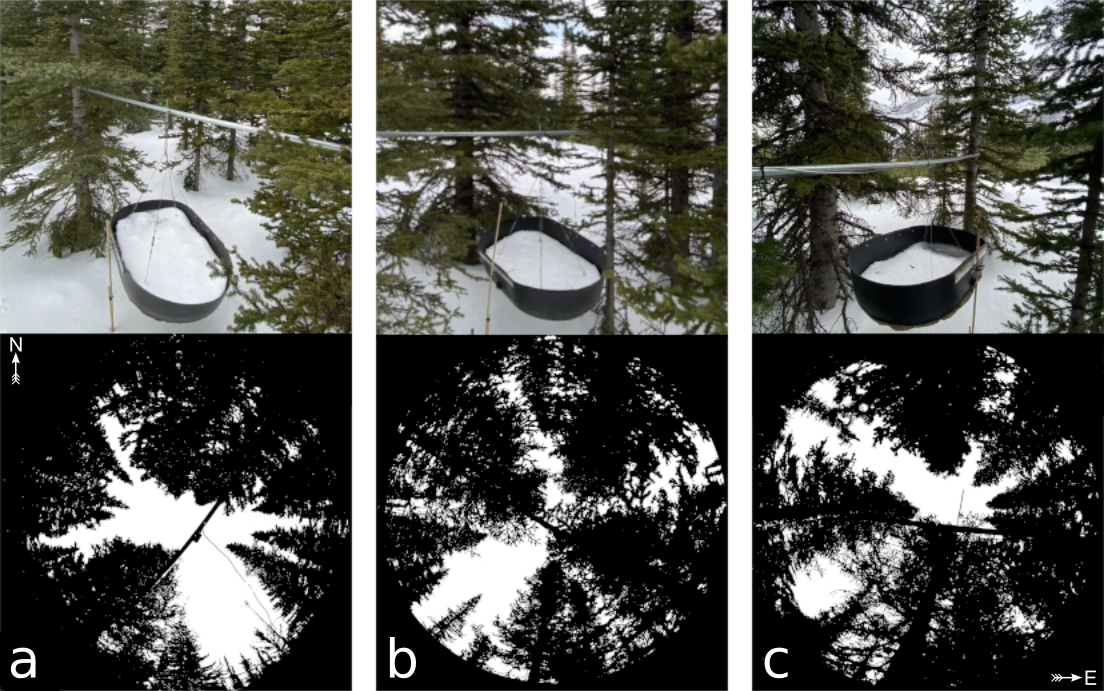
\includegraphics[keepaspectratio]{chapters/03-snow-int-paper/figs/figure2.png}}

}

\caption{\label{fig-scl-imgs}Images of the three subcanopy lysimeter
instruments and surrounding canopy located in sparse (a), mixed (b), and
dense (c) canopy. The top row presents a side view of each instrument
and the bottom row shows hemispherical photographs. These hemispherical
images are oriented with north at the top and have been mirrored to
provide a view from above (e.g., east is on the right side of each
image). See Table~\ref{tbl-scl-lai-cc} for the corresponding canopy
density measurement.}

\end{figure}%

\subsection{UAV-Lidar data collection and
processing}\label{uav-lidar-data-collection-and-processing}

The UAV (FreeFly Alta X) payload included a REIGL miniVUX-2 airborne
laser scanner, an Applanix APX-20 inertial measurement unit (IMU) and
global navigation satellite system (GNSS). The UAV was flown 90 m above
the ground at a speed of 3 m s\textsuperscript{-1} following the path
shown in Figure~\ref{fig-site-map}. The methods outlined by Harder et
al. (2020) and Staines \& Pomeroy (2023) were incorporated to reconcile
survey lidar, IMU, and GNSS data. A systematic vertical bias of up to 6
cm between UAV-lidar flight lines was observed in the resulting point
clouds on March 13\textsuperscript{th} and 14\textsuperscript{th}, 2024
and was attributed to IMU position drift. After strip alignment, the
mean elevation bias in the point clouds compared to the GNSS data was
0.000 m and the RMS error declined from 0.055 m to 0.038 m on March
13\textsuperscript{th} and from 0.033 m to 0.029 m on March
14\textsuperscript{th}. The point cloud density ranged from
\textasciitilde1200 returns m\textsuperscript{2} in sparse forest to
\textasciitilde2200 returns m\textsuperscript{2} in open clearings.
Quality control, ground classification, calculation of surface elevation
change was conducted on the point cloud data and then converted to 0.05
m resolution rasters. Further quality control was conducted on the 0.05
m raster data to remove values that exceeded the .999th quantile and
then resampled to 0.25 m grid cell resolution by taking the median. A
detailed description of the UAV, payload, flight settings, and software
packages used is provided in the Supporting Information.

\subsection{Snow surveys}\label{snow-surveys}

\subsubsection{In-situ snow depth and
density}\label{in-situ-snow-depth-and-density}

Event-based snow surveys provided measurements of subcanopy throughfall
depth and density at 30 locations following the transects shown in
Figure~\ref{fig-site-map}. These measurements were used to upscale the
weighed tree from weight to weight per unit area, assess the accuracy of
lidar derived snow depth measurements, and provide a fresh snow density
for the calculation of SWE (mm) from the snow depth measurements.
Minimal ablation and redistribution of both the surface snowpack and/or
snow intercepted in the canopy was crucial to ensure the snow survey
measurements were attributed to throughfall. Therefore, only snowfall
events with minimal canopy snow ablation as determined through in-situ
observations, analysis of timelapse imagery, and mass change on the
weighed tree lysimeter were selected. A 1000 cm\textsuperscript{3} Perla
snow density wedge sampler (RIP Cutter,
https://snowmetrics.com/shop/rip-1-cutter-1000-cc/) was used to measure
the density of the fresh snow layer, \(\overline{\rho_{tf}}\) (kg
m\textsuperscript{-3}) from snow pits. Throughfall depth measurements,
\(\Delta HS\) were converted to SWE using the following equation:

\begin{equation}\phantomsection\label{eq-swe-tf}{
\Delta SWE_{tf} = \Delta HS \cdot \overline{\rho_{tf}}
}\end{equation}

If a pre-event crust layer was present, the depth of post event fresh
snow accumulation above the crust layer was interpreted as throughfall
over the event. In the absence of a defined crust layer, the difference
in pre- and post-event snow depth to ground was interpreted as event
throughfall. Interception efficiency, used in scaling the weighed tree,
was calculated using Equation~\ref{eq-ip2} and the \(\Delta SWE_{tf}\)
and cumulative snowfall measurements.

\subsubsection{UAV-Lidar snow depth}\label{uav-lidar-snow-depth}

Two uncrewed aerial vehicle (UAV) lidar surveys were conducted before
and after a 24-hour snowfall event that occurred between March
13--14\textsuperscript{th}, 2023 to facilitate the measurement of snow
accumulation and canopy density within the FT and PWL forest plots. This
period was selected based on two criteria: 1) it provided sufficient
cumulative snowfall to result in a low relative error in UAV-lidar
measured throughfall, and 2) minimal snow redistribution and ablation
was observed, as confirmed by the subcanopy lysimeters, weighed tree,
and time-lapse imagery. The change in surface elevation between the two
UAV-lidar point clouds was interpreted as the increase in snow
accumulation, \(\Delta HS\), over the snowfall event.
\(\Delta SWE_{tf}\) was calculated using Equation~\ref{eq-swe-tf}
together with in-situ measurements of \(\overline{\rho_{tf}}\). The
measurement error of the UAV-lidar derived \(\Delta HS\) was assessed
using the in-situ snow depth observations which is shown in the
Supporting Information. Spatially distributed measurements of
\(\frac{I}{P}\), were then determined using Equation~\ref{eq-ip2} with
\(\Delta SWE_{tf}\) as the throughfall component and cumulative snowfall
to the PWL clearing.

\subsection{UAV-Lidar canopy metrics}\label{uav-lidar-canopy-metrics}

The canopy of the study site was characterized from two UAV-lidar point
clouds (March 13\textsuperscript{th} and March 14\textsuperscript{th})
using the voxel ray sampling (VoxRS) methodology for lidar data
analysis, as developed by Staines \& Pomeroy (2023). This method was
chosen for its ability to provide canopy metrics that are less sensitive
to the inherent non-uniform nature of lidar sampling data resulting from
beam occlusion in vegetation. Using this method radiation transmittance,
\(\tau\) (-), was measured across the hemisphere at a 1° step, e.g.,
azimuth angles (0°, 1°, \ldots, 359°) and zenith angles (0°, 1°, \ldots,
90°) for each 0.25 m grid cell within the FT and PWL forest plots. The
fraction of snow-leaf contact area per unit area of ground proposed by
Hedstrom \& Pomeroy (1998), and hereafter called leaf contact area
(\(C_p\)), was then calculated as:

\begin{equation}\phantomsection\label{eq-lca}{
C_p(C_c, \theta_h) = 1-\tau
}\end{equation}

\begin{equation}\phantomsection\label{eq-tf-ode}{
C_p(C_c, \theta_h) = \begin{cases}
    1-\tau,& \text{if } \theta_h> 0°\\
    1-\tau \approx C_c ,              & \theta_h= 0°
\end{cases}
}\end{equation}

where \(C_p\) is a function of the canopy cover (\(C_c\)) and
hydrometeor trajectory angle (\(\theta_h\)). \(C_c\) is the fraction of
canopy area to total ground area when viewed from above, which differs
from canopy closure, an angular-derived metric usually measured from the
ground perspective.

To determine how \(C_p\) was associated with interception efficiency at
different azimuth and zenith angles over the March
13--14\textsuperscript{th} snowfall event, the entire hemisphere at each
grid location was considered. The relationship between interception
efficiency and \(C_p\) was found to be linear and thus the Pearson
Correlation Coefficient was used. The Pearson Correlation Coefficient
was computed between a single raster of interception efficiency and each
of the 32,760 rasters of \(C_p\) measured on March
13\textsuperscript{th}, representing locations across the hemisphere
(azimuth {[}0°, 1°, \ldots, 359°{]}, zenith angle {[}0°, 1°, \ldots,
90°{]}) at 0.25 m grid cells spanning the FT and PWL forest plots.

The pair of azimuth and zenith angles corresponding to the \(C_p\) that
had the highest correlation with interception efficiency was selected
for further analysis. This involved aggregating the interception
efficiency and selected \(C_p\) rasters from a 0.25 m resolution to 5 m,
followed by fitting an ordinary least squares regression between these
two variables. The regression was constrained to pass through the origin
based on the theoretical principle that the dependent variable must
equal zero when the independent variable is zero. To appropriately
account for this constraint, the \emph{R}\textsuperscript{2} values were
adjusted according to Equation 10 presented in Kozak \& Kozak (1995).
The relationship between leaf contact area and simulated trajectory
angle was investigated by fitting non-linear models using a non-linear
least squares regression. All statistical analyses were performed using
the R `stats' package (R Core Team, 2024).

\section{Results}\label{results}

\subsection{The influence of meteorology on snow
interception}\label{the-influence-of-meteorology-on-snow-interception}

Measurements of canopy snow load derived from the subcanopy lysimeters
and weighed tree increased linearly with cumulative event snowfall for
26 snowfall events, without evidence of reaching a maximum
(Figure~\ref{fig-scl-w-sf}). Over these events, air temperature ranged
from -24.5°C to 1°C, wind speeds at 4.3 m height ranged from calm to 4.6
m s\textsuperscript{-1} (Table~\ref{tbl-sf-event-met}), and wind
direction was predominately from the southwest during snowfall
(Figure~\ref{fig-wind-rose}). Missing canopy snow load measurements, as
shown in Figure~\ref{fig-scl-w-sf} for certain events, were caused by
wiring damage from animals and heavy snow loads. Some of the variability
in interception rates within and between different events may be
attributed to small amounts of canopy snow unloading and melt, which
could not be fully accounted for through the manual and automated
filtering mitigation strategies in both the subcanopy lysimeter and
weighed tree measurements.

\begin{figure}

\centering{

\pandocbounded{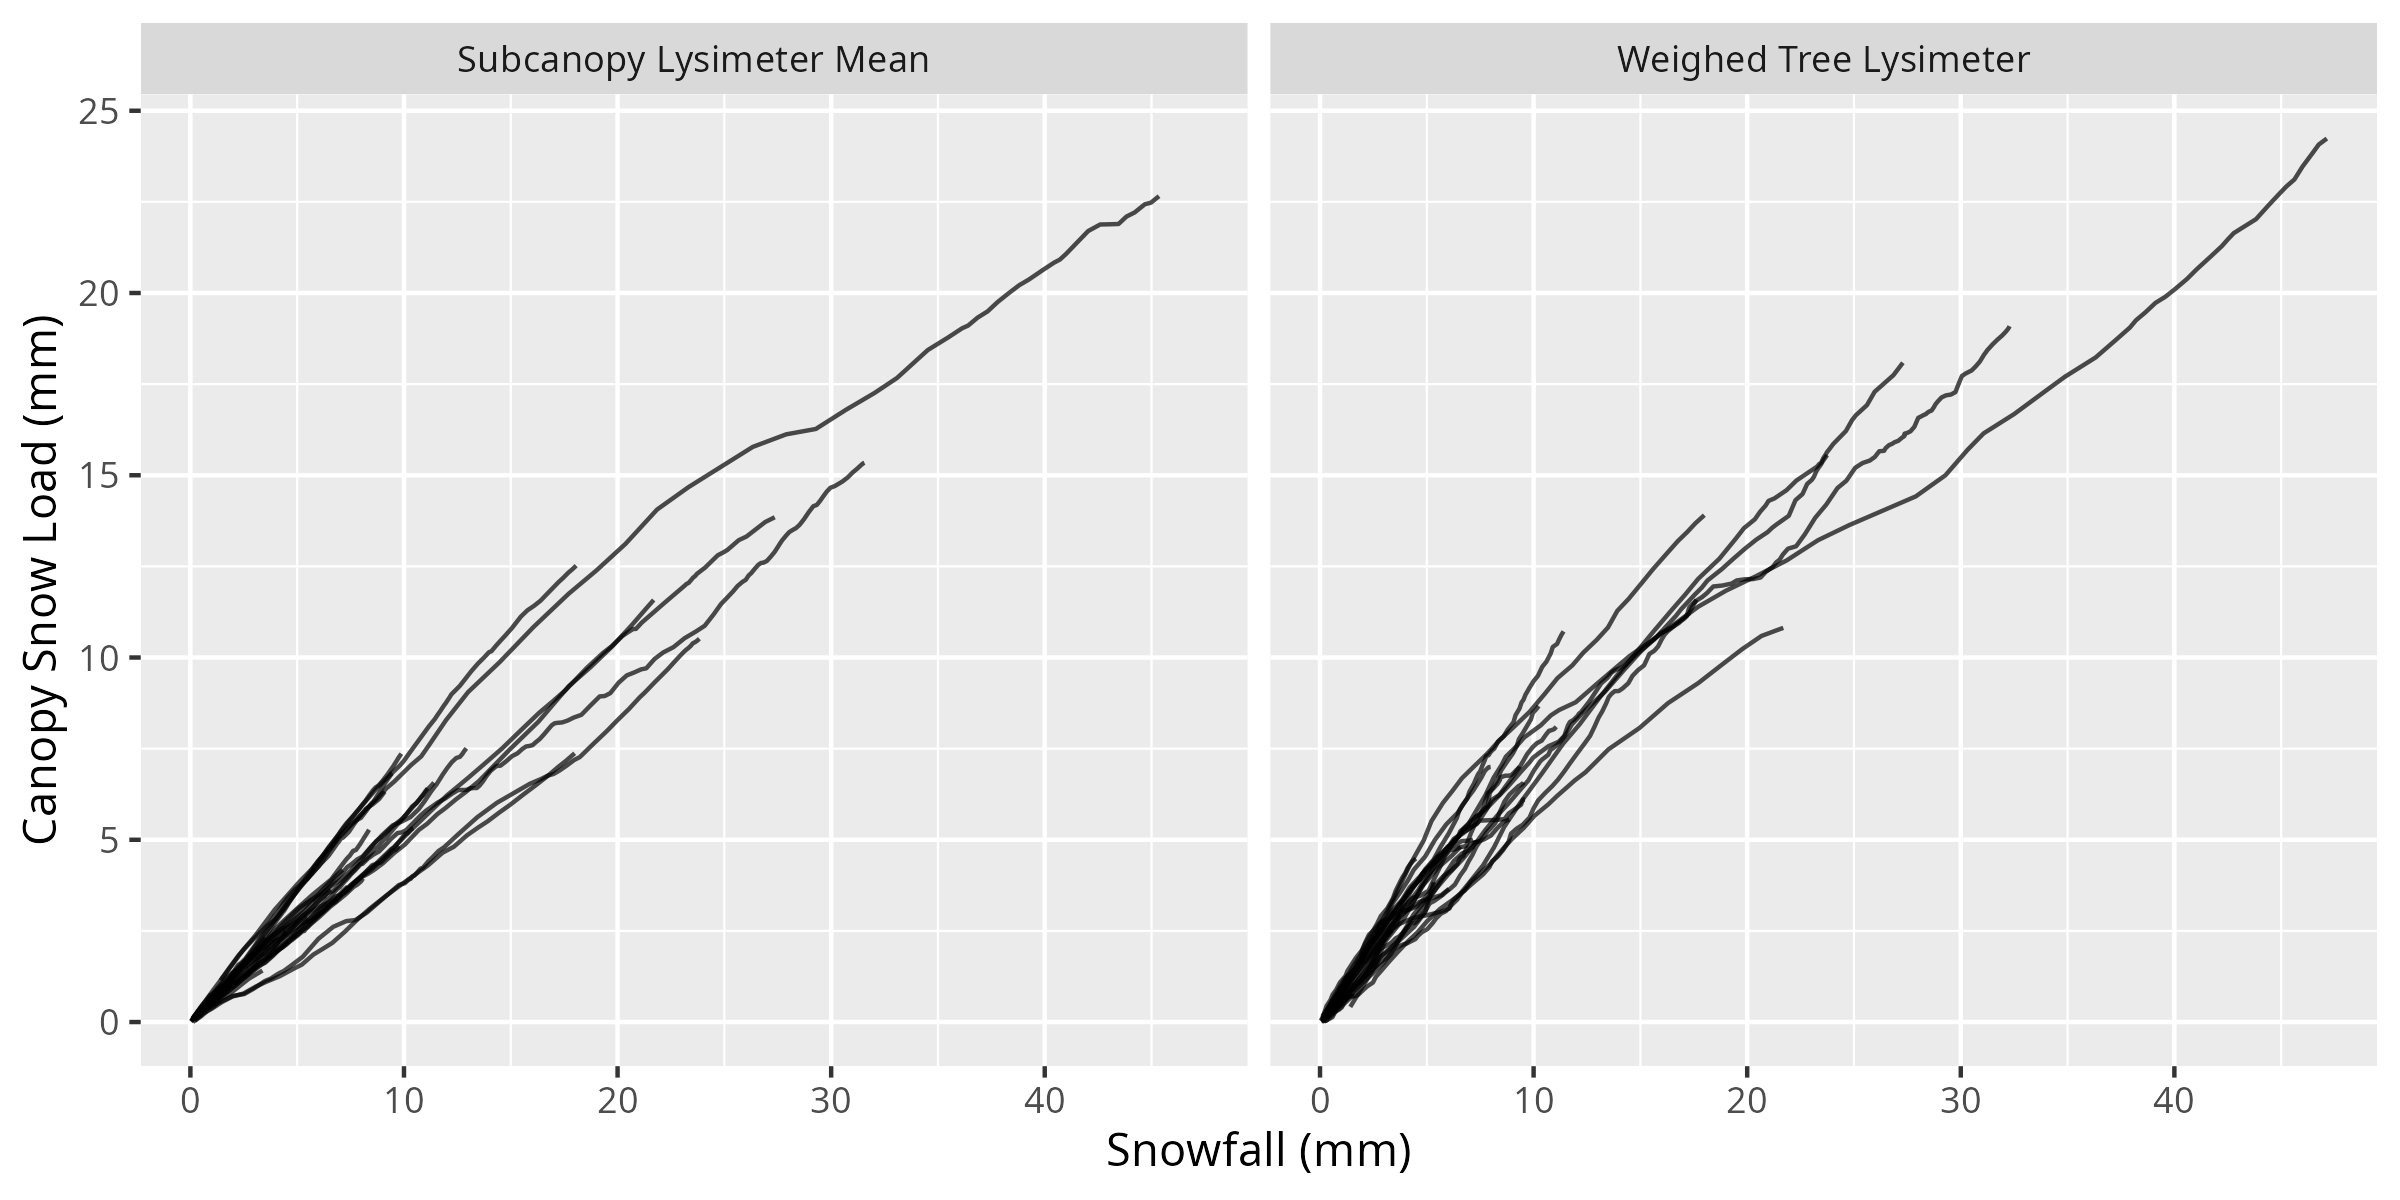
\includegraphics[keepaspectratio]{chapters/03-snow-int-paper/figs/figure3.png}}

}

\caption{\label{fig-scl-w-sf}Plot showing the cumulative event snowfall
versus canopy snow load calculated using the mean of the three subcanopy
lysimeters (left) and weighed tree lysimeter (right) for each of the 26
snowfall events. Both datasets represent canopy snow load for a canopy
closure of 0.73 corresponding to the mean of the three subcanopy
lysimeter canopies.}

\end{figure}%

\pagebreak

\begin{table}

\caption{\label{tbl-sf-event-met}Meteorology of the 26 snowfall events.
Air temperature and wind speed were measured at FT station. Interception
efficiency is estimated from cumulative snowfall measured at PWL station
and the average cumulative throughfall of all three subcanopy lysimeters
located within the FT forest plot.}

\centering{

\fontsize{12.0pt}{14.4pt}\selectfont
\begin{tabular*}{\linewidth}{@{\extracolsep{\fill}}>{\centering\arraybackslash}p{\dimexpr 67.50pt -2\tabcolsep-1.5\arrayrulewidth}>{\centering\arraybackslash}p{\dimexpr 37.50pt -2\tabcolsep-1.5\arrayrulewidth}>{\centering\arraybackslash}p{\dimexpr 37.50pt -2\tabcolsep-1.5\arrayrulewidth}>{\centering\arraybackslash}p{\dimexpr 37.50pt -2\tabcolsep-1.5\arrayrulewidth}>{\centering\arraybackslash}p{\dimexpr 37.50pt -2\tabcolsep-1.5\arrayrulewidth}>{\centering\arraybackslash}p{\dimexpr 37.50pt -2\tabcolsep-1.5\arrayrulewidth}>{\centering\arraybackslash}p{\dimexpr 37.50pt -2\tabcolsep-1.5\arrayrulewidth}>{\centering\arraybackslash}p{\dimexpr 37.50pt -2\tabcolsep-1.5\arrayrulewidth}>{\centering\arraybackslash}p{\dimexpr 37.50pt -2\tabcolsep-1.5\arrayrulewidth}>{\centering\arraybackslash}p{\dimexpr 37.50pt -2\tabcolsep-1.5\arrayrulewidth}>{\centering\arraybackslash}p{\dimexpr 60.00pt -2\tabcolsep-1.5\arrayrulewidth}}
\toprule
 & \multicolumn{3}{>{\centering\arraybackslash}m{\dimexpr 112.50pt -2\tabcolsep-1.5\arrayrulewidth}}{Air Temperature (°C)} & \multicolumn{3}{>{\centering\arraybackslash}m{\dimexpr 112.50pt -2\tabcolsep-1.5\arrayrulewidth}}{Wind Speed (m/s)} & \multicolumn{3}{>{\centering\arraybackslash}m{\dimexpr 112.50pt -2\tabcolsep-1.5\arrayrulewidth}}{Interception Efficiency (-)} & Snowfall (mm) \\ 
\cmidrule(lr){2-4} \cmidrule(lr){5-7} \cmidrule(lr){8-10} \cmidrule(lr){11-11}
Start Date & Min & Mean & Max & Min & Mean & Max & Min & Mean & Max & Total \\ 
\midrule\addlinespace[2.5pt]
2021-12-23 & -6.2 & -5.3 & -4.6 & 0.6 & 3.1 & 4.6 & 0.1 & 0.5 & 0.9 & 21.7 \\ 
2022-01-02 & -15.9 & -10.8 & -5.8 & 0.2 & 1.8 & 4.2 & 0.0 & 0.5 & 1.0 & 31.6 \\ 
2022-01-17 & -14.8 & -7.8 & -0.8 & 0.2 & 1.1 & 1.8 & 0.0 & 0.6 & 1.0 & 12.9 \\ 
2022-01-31 & -24.5 & -12.1 & -6.4 & 0.1 & 1.0 & 1.7 & 0.2 & 0.7 & 1.0 & 9.1 \\ 
2022-02-14 & -9.9 & -9.0 & -8.5 & 0.4 & 0.8 & 1.2 & 0.2 & 0.5 & 0.8 & 1.7 \\ 
2022-02-19 & -4.7 & -3.2 & -2.5 & 1.3 & 2.3 & 3.6 & 0.3 & 0.6 & 0.9 & 11.1 \\ 
2022-03-01 & -8.3 & -5.4 & -1.0 & 0.1 & 1.0 & 3.1 & 0.4 & 0.8 & 1.0 & 9.9 \\ 
2022-03-07 & -12.5 & -8.6 & -4.4 & 0.3 & 0.8 & 1.7 & 0.3 & 0.7 & 1.0 & 9.5 \\ 
2022-03-14 & -2.7 & -2.1 & -0.8 & 1.0 & 1.6 & 2.9 & 0.2 & 0.6 & 0.9 & 8.4 \\ 
2022-03-19 & -3.1 & -2.8 & -2.5 & 0.0 & 0.7 & 1.3 & 0.3 & 0.5 & 0.6 & 6.6 \\ 
2022-03-23 & -7.9 & -5.3 & -0.9 & 0.8 & 1.2 & 1.8 & 0.4 & 0.6 & 0.9 & 1.6 \\ 
2022-04-04 & -3.5 & -2.9 & -2.1 & 0.6 & 1.0 & 1.9 & 0.0 & 0.4 & 0.6 & 3.4 \\ 
2022-04-18 & -5.2 & -4.0 & -2.7 & 0.4 & 1.1 & 1.9 & 0.1 & 0.5 & 0.9 & 7.4 \\ 
2022-04-22 & -2.8 & -1.8 & -0.5 & 0.4 & 0.8 & 1.2 & 0.1 & 0.5 & 1.0 & 9.8 \\ 
2022-05-09 & -4.9 & -4.3 & -3.2 & 0.1 & 0.4 & 0.9 & 0.2 & 0.5 & 0.9 & 8.1 \\ 
2022-05-19 & -4.9 & -2.1 & 0.3 & 0.1 & 0.4 & 0.9 & 0.2 & 0.6 & 0.9 & 7.1 \\ 
2022-06-13 & -1.1 & -0.3 & 0.6 & 0.1 & 0.1 & 0.4 & 0.0 & 0.5 & 0.9 & 45.4 \\ 
2022-12-27 & -3.0 & -2.7 & -1.9 & 0.6 & 1.1 & 1.8 & 0.2 & 0.5 & 0.9 & 4.5 \\ 
2023-01-27 & -11.5 & -7.3 & -4.5 & 0.6 & 0.9 & 1.2 & 0.1 & 0.5 & 0.8 & 10.4 \\ 
2023-02-19 & -14.3 & -9.5 & -6.3 & 0.2 & 0.8 & 1.4 & 0.2 & 0.7 & 1.0 & 18.1 \\ 
2023-02-26 & -9.2 & -8.4 & -6.6 & 0.2 & 1.0 & 2.1 & 0.3 & 0.5 & 1.0 & 5.4 \\ 
2023-03-13 & -8.9 & -3.6 & -0.1 & 0.3 & 1.3 & 2.2 & 0.0 & 0.5 & 1.0 & 27.4 \\ 
2023-03-24 & -7.9 & -5.7 & -3.5 & 0.1 & 0.5 & 1.2 & 0.1 & 0.4 & 0.7 & 23.8 \\ 
2023-04-01 & -8.9 & -7.7 & -4.7 & 0.1 & 0.6 & 1.4 & 0.4 & 0.6 & 0.8 & 11.4 \\ 
2023-04-10 & -1.1 & -0.5 & 0.3 & 0.1 & 0.3 & 1.0 & 0.2 & 0.4 & 0.6 & 18.0 \\ 
2023-05-08 & 0.2 & 0.6 & 1.0 & 0.4 & 0.6 & 0.8 & 0.6 & 0.6 & 0.7 & 3.5 \\ 
\bottomrule
\end{tabular*}

}

\end{table}%

\begin{figure}

\centering{

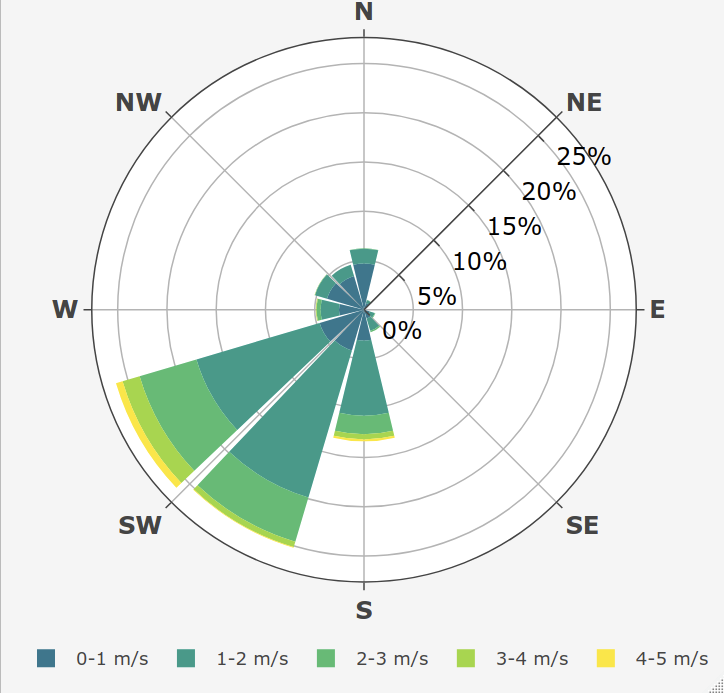
\includegraphics[width=0.6\linewidth,height=\textheight,keepaspectratio]{chapters/03-snow-int-paper/figs/figure4.png}

}

\caption{\label{fig-wind-rose}Wind rose showing the frequency of wind
speed and direction over the 26 snowfall periods for the ultrasonic
anemometer 4.3 m above ground at FT station.}

\end{figure}%

Linear regression analysis revealed no relationship between hourly
interception efficiency (from the subcanopy lysimeters) and air
temperature, wind speed or canopy snow load, either due to
non-significant relationships (\emph{p} \textless{} 0.05) and/or weak
predictive power (\emph{R}\textsuperscript{2} \textless{} 0.05)
(Table~\ref{tbl-lysimeter-hourly-stats}). The Wilcoxon test indicated
that the difference in hourly interception efficiencies for air
temperatures above and below -5°C was not significant (\emph{p}
\textgreater{} 0.05, Table~\ref{tbl-scl-hrly-stats}). Additionally, the
interception efficiency across differing bins of air temperature did not
show any systematic pattern (Figure~\ref{fig-scl-ip-bins}). Although
Figure~\ref{fig-scl-ip-bins} indicates potentially higher interception
efficiency in sparse and mixed canopies at air temperatures below -10°C,
these measurements have substantial uncertainty due to heightened
instrument error associated with the small accumulations of snowfall and
throughfall within these temperature ranges.

When examining wind speed effects, hourly interception efficiencies were
found to be significantly higher (\emph{p} \textless{} 0.05,
Table~\ref{tbl-scl-hrly-stats}) during periods when wind speeds exceeded
1 m s\textsuperscript{-1} compared to calmer conditions in the sparse
and closed canopies using the Wilcoxon test. The binned data also show
an increase in interception efficiency with increasing wind speed for
these two canopy types (Figure~\ref{fig-scl-ip-bins}). In contrast, the
mixed canopy, which had a canopy opening towards the prevailing wind
direction (Figure~\ref{fig-scl-imgs}), exhibited no significant
difference (\emph{p} \textgreater{} 0.05,
Table~\ref{tbl-scl-hrly-stats}). Binned measurements of interception
efficiencies corresponding to wind speed bins above 2 m
s\textsuperscript{-1} (Figure~\ref{fig-scl-ip-bins}) contained
considerable uncertainty resulting from lower snowfall and throughfall
accumulation, reducing confidence in these particular findings across
all three canopy environments.

Significantly higher hourly interception efficiencies (\emph{p}
\textless{} 0.05, Table~\ref{tbl-scl-hrly-stats}) were found for initial
canopy snow loads below 10 mm compared to heavier snow loads across all
three canopy types using the Wilcoxon test. Additionally, the sparse and
mixed canopies exhibited significantly lower interception efficiencies
(\emph{p} \textless{} 0.05) for snow loads below 5 mm compared to those
between 5--10 mm. The closed canopy displayed a similar initial increase
for the binned data visible in Figure~\ref{fig-scl-ip-bins}, but this
was not statistically significant for the hourly data (\emph{p}
\textgreater{} 0.05, Table~\ref{tbl-scl-hrly-stats}). For the sparse and
closed canopies, a slight increase in binned interception efficiency was
observed as snow load increased up to 10 mm, followed by a decline when
snow loads exceeded 10 mm (Figure~\ref{fig-scl-ip-bins}). For snow loads
exceeding 15 mm, interception efficiency decreased in the sparse and
closed canopies, while the mixed canopy showed an increase; however,
these measurements carried high uncertainties due to lower accumulated
snowfall and throughfall in these higher snow load bins. The differences
between the relationships observed in the hourly-interval and binned
interception efficiency measurements can be attributed to two factors:
greater instrument uncertainty in the hourly measurements and the
potential for the dependent and independent variables to be
non-stationary over the hourly interval.

\begin{longtable}[]{@{}
  >{\raggedright\arraybackslash}p{(\linewidth - 10\tabcolsep) * \real{0.3500}}
  >{\raggedright\arraybackslash}p{(\linewidth - 10\tabcolsep) * \real{0.1500}}
  >{\raggedleft\arraybackslash}p{(\linewidth - 10\tabcolsep) * \real{0.1000}}
  >{\raggedleft\arraybackslash}p{(\linewidth - 10\tabcolsep) * \real{0.1700}}
  >{\raggedleft\arraybackslash}p{(\linewidth - 10\tabcolsep) * \real{0.1300}}
  >{\raggedleft\arraybackslash}p{(\linewidth - 10\tabcolsep) * \real{0.1000}}@{}}

\caption{\label{tbl-lysimeter-hourly-stats}Statistics corresponding to
the ordinary least squares linear regression test between hourly
interval measurements of independent variables: mean air temperature,
mean wind speed, and initial canopy snow load and the dependent variable
mean interception efficiency. The test was run separately for three
levels of canopy coverage (\(C_c\)) corresponding to each subcanopy
lysimeter (SCL).}

\tabularnewline

\toprule\noalign{}
\begin{minipage}[b]{\linewidth}\raggedright
Dependent Variable
\end{minipage} & \begin{minipage}[b]{\linewidth}\raggedright
SCL Name
\end{minipage} & \begin{minipage}[b]{\linewidth}\raggedleft
\(C_c\)
\end{minipage} & \begin{minipage}[b]{\linewidth}\raggedleft
Adjusted \(R^2\)
\end{minipage} & \begin{minipage}[b]{\linewidth}\raggedleft
\(p\)-value
\end{minipage} & \begin{minipage}[b]{\linewidth}\raggedleft
\(n\)
\end{minipage} \\
\midrule\noalign{}
\endhead
\bottomrule\noalign{}
\endlastfoot
Air Temperature (°C) & closed & 0.79 & 0.002 & 0.239 & 191 \\
Air Temperature (°C) & mixed & 0.75 & 0.024 & 0.005 & 298 \\
Air Temperature (°C) & sparse & 0.64 & 0.003 & 0.208 & 190 \\
Initial Canopy Snow Load (mm) & closed & 0.79 & 0.029 & 0.011 & 188 \\
Initial Canopy Snow Load (mm) & mixed & 0.75 & 0.010 & 0.049 & 294 \\
Initial Canopy Snow Load (mm) & sparse & 0.64 & 0.031 & 0.009 & 187 \\
Wind Speed (m/s) & closed & 0.79 & 0.025 & 0.017 & 191 \\
Wind Speed (m/s) & mixed & 0.75 & 0.034 & 0.001 & 298 \\
Wind Speed (m/s) & sparse & 0.64 & 0.046 & 0.002 & 190 \\

\end{longtable}

\begin{figure}

\centering{

\pandocbounded{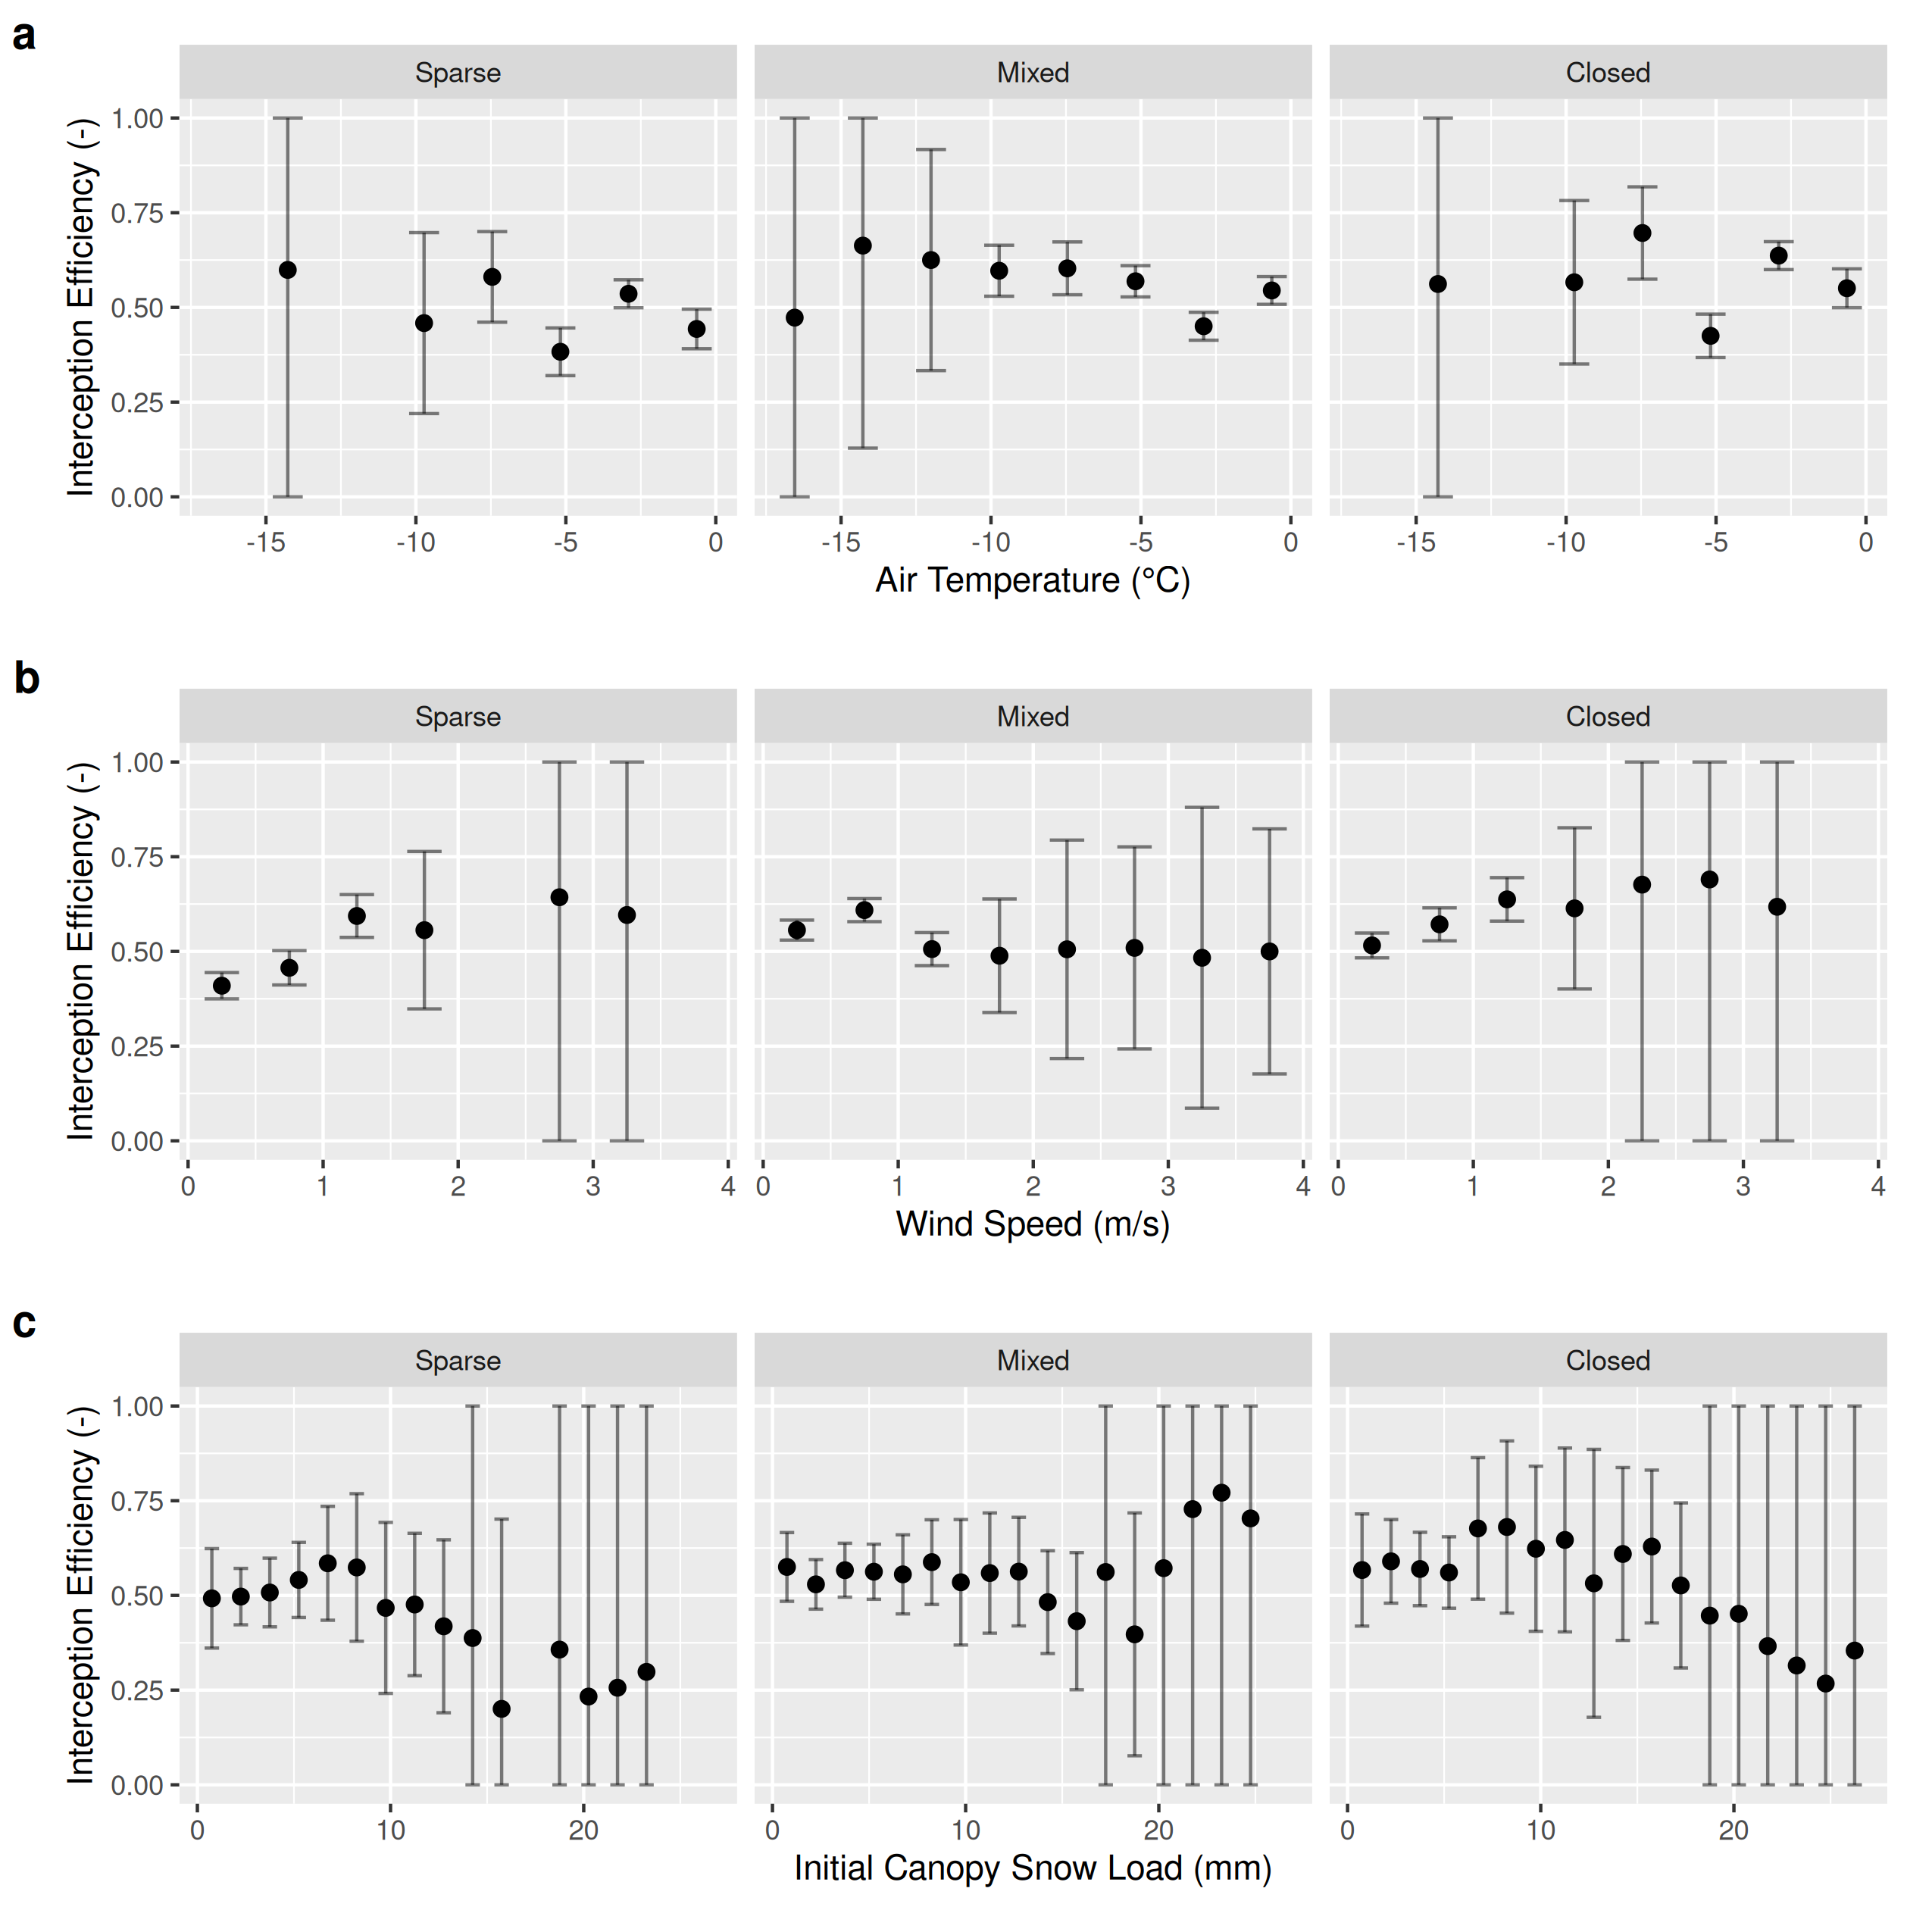
\includegraphics[keepaspectratio]{chapters/03-snow-int-paper/figs/figure5.png}}

}

\caption{\label{fig-scl-ip-bins}Scatter plots showing the interception
efficiency calculated from accumulated snowfall (Pluvio) and throughfall
(subcanopy lysimeter) measurements for bins of air temperature, wind
speed, and initial canopy snow load (the snow load observed by the
weighed tree at the beginning of the timestep) over the 26 snowfall
events. The error bars represent the estimated combined instrument error
of the snowfall gauge and subcanopy lysimeters.}

\end{figure}%

\begin{longtable}[]{@{}
  >{\raggedright\arraybackslash}p{(\linewidth - 10\tabcolsep) * \real{0.1200}}
  >{\raggedright\arraybackslash}p{(\linewidth - 10\tabcolsep) * \real{0.3000}}
  >{\raggedright\arraybackslash}p{(\linewidth - 10\tabcolsep) * \real{0.1200}}
  >{\raggedright\arraybackslash}p{(\linewidth - 10\tabcolsep) * \real{0.1800}}
  >{\raggedright\arraybackslash}p{(\linewidth - 10\tabcolsep) * \real{0.1500}}
  >{\raggedright\arraybackslash}p{(\linewidth - 10\tabcolsep) * \real{0.1300}}@{}}

\caption{\label{tbl-scl-hrly-stats}Results of the Wilcoxon signed-rank
tests comparing the distributions of hourly interception efficiency (IP)
measured by the subcanopy lysimeters for differing groups of air
temperatures (Ta), wind speeds (u), and initial canopy snow loads (L).
The table reports the canopy corresponding to the subcanopy lysimeter
(Canopy), null hypothesis (\(H_0\)), \(p\)-value, and sample size
(\(n\)) and median IP for the `low' group (e.g., Ta \textless{} -5°C)
and `high' group (e.g., Ta ≥ -5°C).}

\tabularnewline

\toprule\noalign{}
\begin{minipage}[b]{\linewidth}\raggedright
Canopy
\end{minipage} & \begin{minipage}[b]{\linewidth}\raggedright
Null Hypothesis (\(H_0\))
\end{minipage} & \begin{minipage}[b]{\linewidth}\raggedright
\(p\)-value
\end{minipage} & \begin{minipage}[b]{\linewidth}\raggedright
\(n\) (low / high)
\end{minipage} & \begin{minipage}[b]{\linewidth}\raggedright
median I/P (low / high)
\end{minipage} & \begin{minipage}[b]{\linewidth}\raggedright
Reject \(H_0\)
\end{minipage} \\
\midrule\noalign{}
\endhead
\bottomrule\noalign{}
\endlastfoot
closed & Median IP (Ta \textless{} -5°C) ≥ Median IP (Ta ≥ -5°C) & 0.282
& 76 / 115 & 0.56 / 0.62 & no \\
mixed & Median IP (Ta \textless{} -5°C) ≥ Median IP (Ta ≥ -5°C) & 0.990
& 165 / 133 & 0.57 / 0.53 & no \\
sparse & Median IP (Ta \textless{} -5°C) ≥ Median IP (Ta ≥ -5°C) & 0.864
& 72 / 118 & 0.54 / 0.5 & no \\
closed & Median IP (u \textless{} 1 m/s) ≥ Median IP (u ≥ 1 m/s) & 0.004
& 116 / 75 & 0.53 / 0.65 & yes \\
mixed & Median IP (u \textless{} 1 m/s) ≥ Median IP (u ≥ 1 m/s) & 1.000
& 165 / 133 & 0.6 / 0.5 & no \\
sparse & Median IP (u \textless{} 1 m/s) ≥ Median IP (u ≥ 1 m/s) &
\textless{} 0.001 & 110 / 80 & 0.43 / 0.59 & yes \\
closed & Median IP (L \textless{} 10 mm) ≤ Median IP (L ≥ 10 mm) & 0.048
& 129 / 59 & 0.62 / 0.57 & yes \\
mixed & Median IP (L \textless{} 10 mm) ≤ Median IP (L ≥ 10 mm) &
\textless{} 0.001 & 218 / 76 & 0.57 / 0.49 & yes \\
sparse & Median IP (L \textless{} 10 mm) ≤ Median IP (L ≥ 10 mm) &
\textless{} 0.001 & 157 / 30 & 0.53 / 0.34 & yes \\
closed & Median IP (L \textless{} 5 mm) ≥ Median IP (5 mm ≤ L
\textless{} 10 mm) & 0.333 & 62 / 67 & 0.62 / 0.62 & no \\
mixed & Median IP (L \textless{} 5 mm) ≥ Median IP (5 mm ≤ L \textless{}
10 mm) & 0.019 & 117 / 101 & 0.57 / 0.61 & yes \\
sparse & Median IP (L \textless{} 5 mm) ≥ Median IP (5 mm ≤ L
\textless{} 10 mm) & 0.043 & 90 / 67 & 0.49 / 0.6 & yes \\

\end{longtable}

\subsection{The influence of canopy density on snow
interception}\label{the-influence-of-canopy-density-on-snow-interception}

UAV-lidar measurements of throughfall and canopy density provide
insights on how the forest canopy influenced subcanopy snow accumulation
during a wind-driven snowfall event between March
13--14\textsuperscript{th}. This event totaled 28.7 mm of snowfall at
PWL station and was characterized by a transition from low rates of
snowfall and air temperatures near 0°C to higher rates of snowfall by
late afternoon on March 13\textsuperscript{th} coinciding with air
temperatures around -2.5 °C. An average wind speed of 1.3 m
s\textsuperscript{-1} and direction of 188° was observed 4.3 m above the
ground at FT Station. The mean observed hydrometeor terminal fall
velocity observed over the event was 0.9 m s\textsuperscript{-1}.

The throughfall depth measured by UAV-lidar aligned with the in-situ
manual measurements resulting in a mean bias of -0.001 m and RMSE of
0.024 m. More details on the accuracy of UAV-lidar snow depth
measurements are provided in the Supporting Information section.
Figure~\ref{fig-lidar-tf-ip} shows the spatial distribution of
throughfall and interception efficiency at the PWL and FT forest plots.
Reduced throughfall and greater interception efficiency was observed on
the north (lee) side of individual trees, which may be due to
non-vertical hydrometeor trajectories caused by the steady southerly
winds observed over this event. Transparent areas within the forest
plots in Figure~\ref{fig-lidar-tf-ip} represent grid cells that did not
have any lidar ground returns (e.g., under dense canopy proximal to tree
trunks) or were masked due to disturbance (e.g., walking paths in
clearings). Visual observations on March 13\textsuperscript{th} and
14\textsuperscript{th} confirmed non-vertical hydrometeor trajectories
and increased canopy snow loads were observed on the windward side of
individual trees. This effect is more apparent in the PWL forest plot
than the FT forest plot and may be attributed to the taller trees and
higher canopy cover of the PWL forest plot compared to the FT forest
plot (Figure~\ref{fig-lidar-tf-ip}).

\begin{figure}

\centering{

\pandocbounded{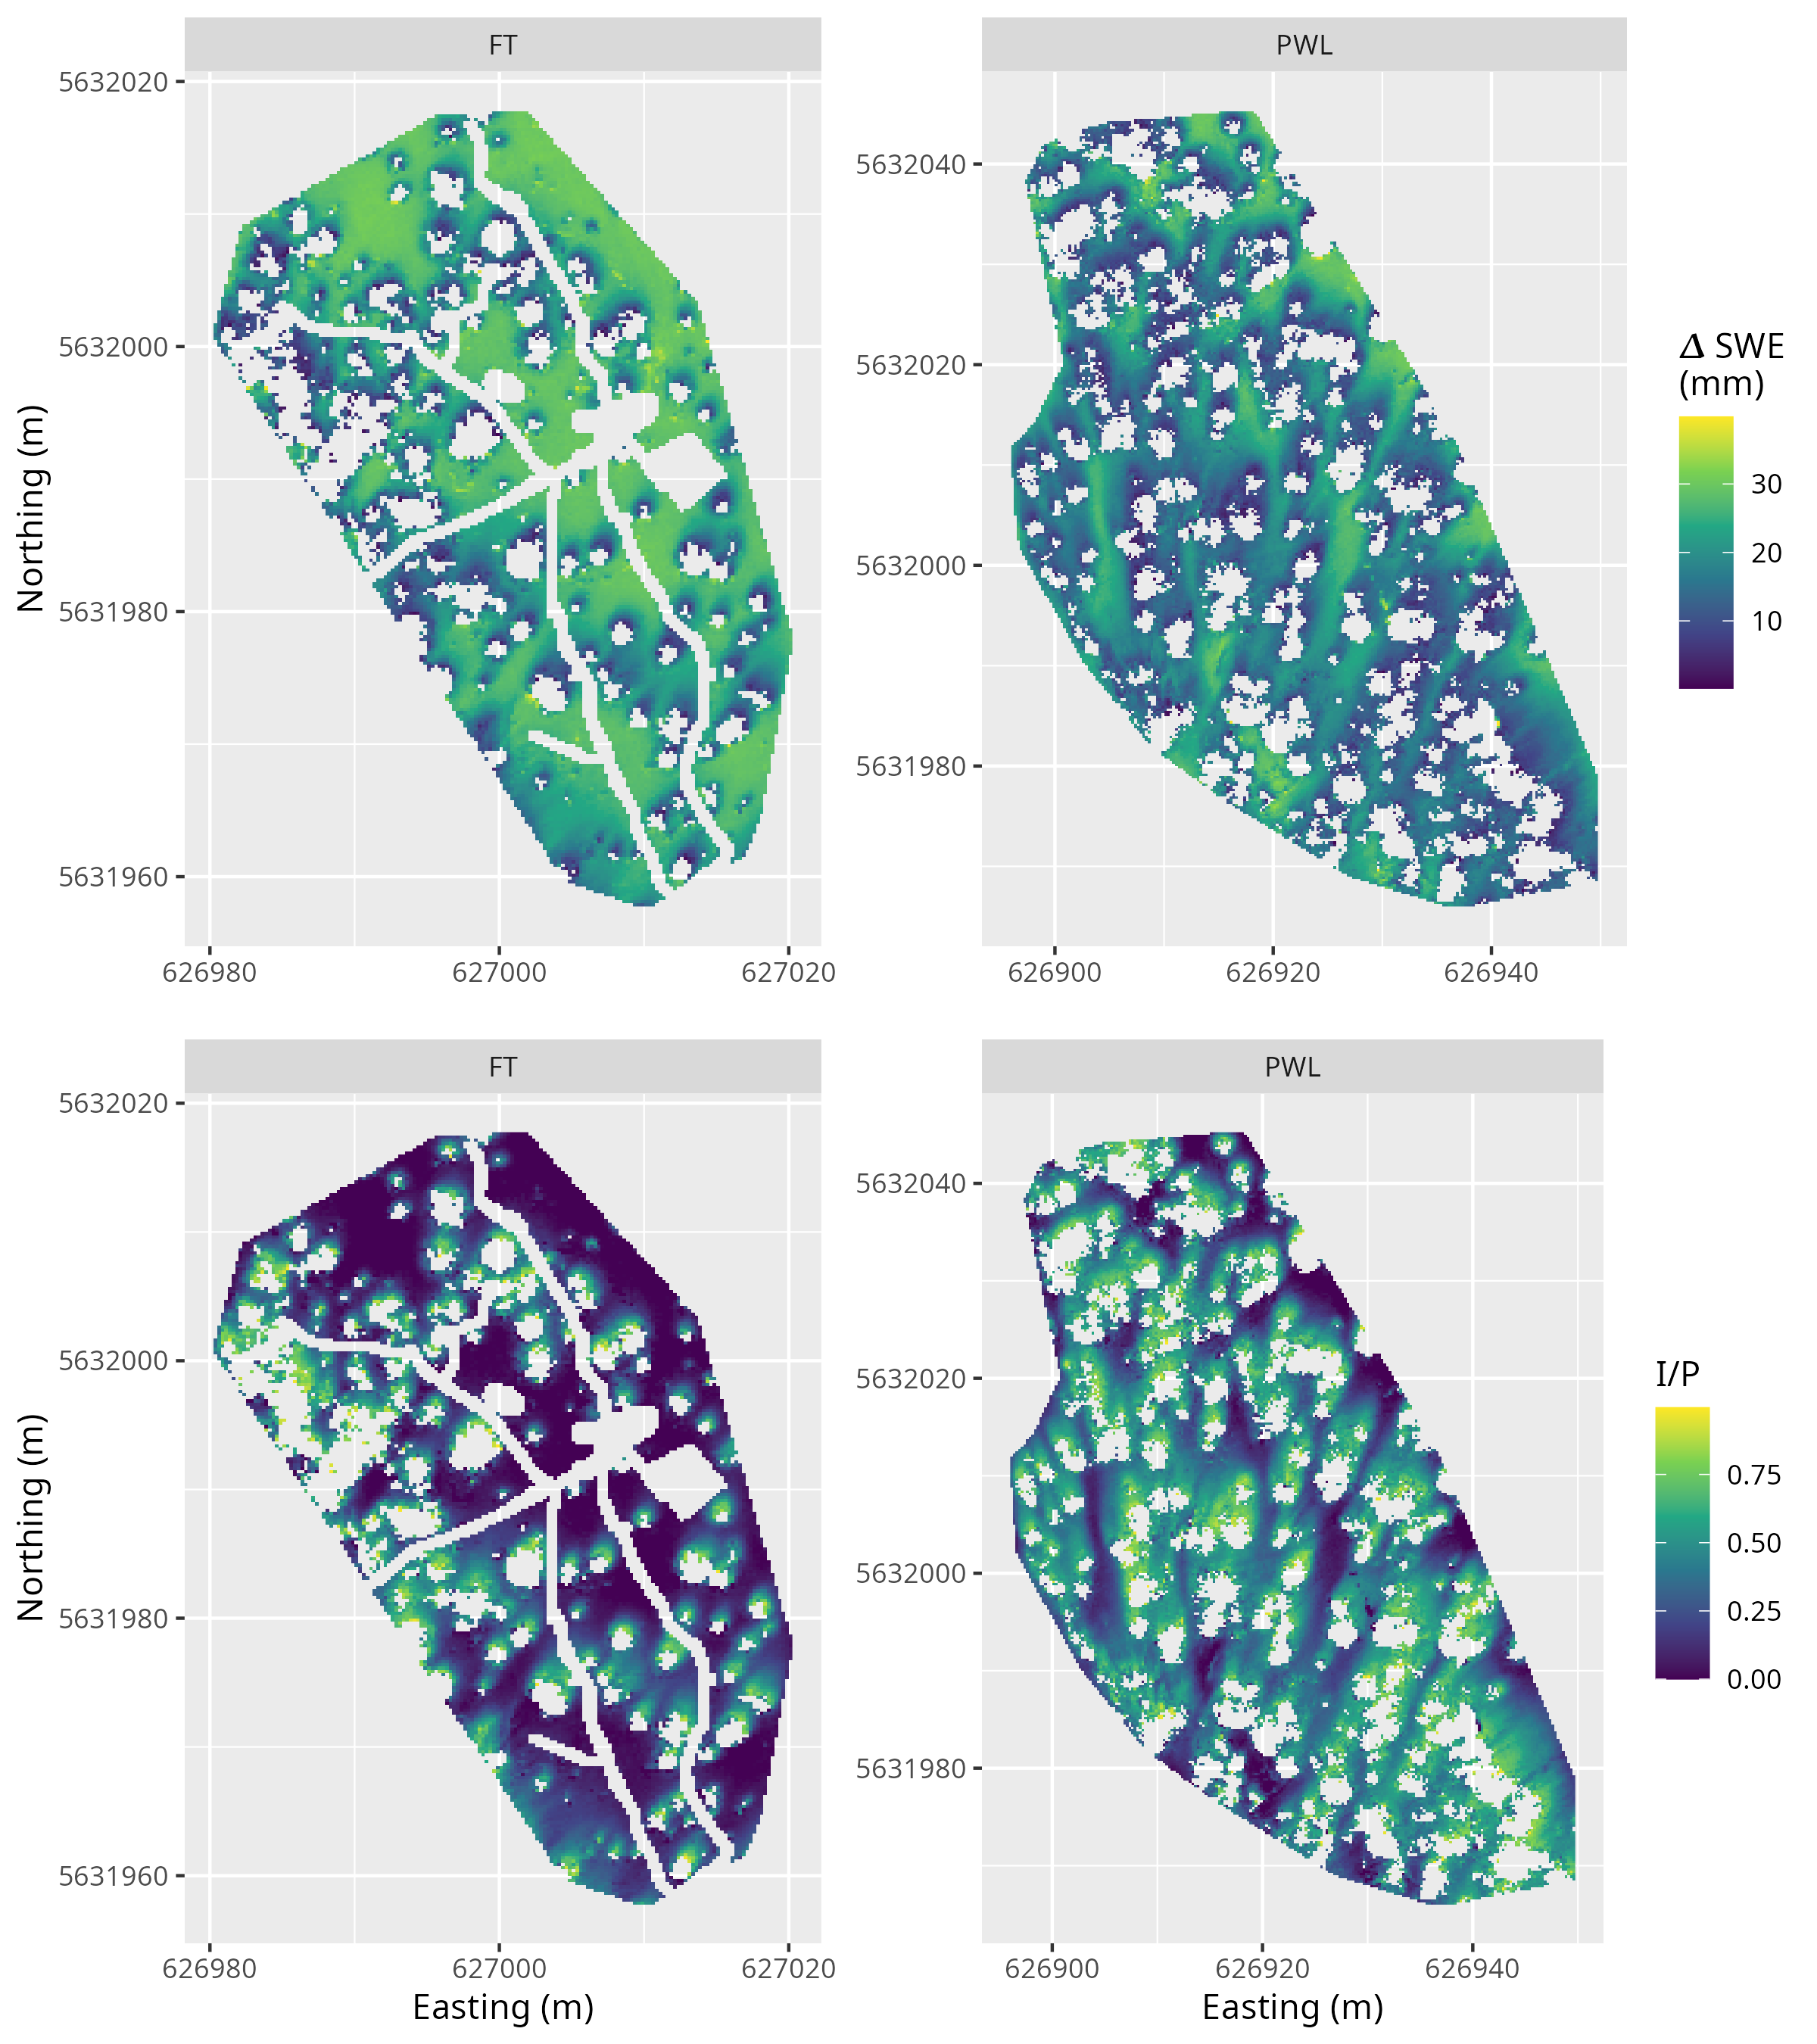
\includegraphics[keepaspectratio]{chapters/03-snow-int-paper/figs/figure6.png}}

}

\caption{\label{fig-lidar-tf-ip}UAV-lidar measurements of the change in
snow water equivalent, SWE (mm) and interception efficiency, I/P (-),
over the March 13--14\textsuperscript{th} 24-hour snowfall event for the
FT and PWL forest plots at a 0.25 m resolution. See the location of the
two forest plots in Figure~\ref{fig-site-map}.}

\end{figure}%

The VoxRS measurements of \(C_p\) on March 13\textsuperscript{th} were
selected for analysis and represent the canopy of both forest plots
without snow. Little difference in \(C_p\) was observed between the
March 13\textsuperscript{th} and March 14\textsuperscript{th}
measurements. A strong linear correlation between \(C_p\) measured on
March 13\textsuperscript{th} and interception efficiency was observed
towards the southern portion of the hemisphere, aligning with the
average event wind direction (Figure~\ref{fig-hemi-ip-cc}). For the PWL
forest plot, the upper 97.5\textsuperscript{th} percentile of the
Pearson Correlation Coefficient (\(\rho_p\)) values were found between
azimuth angles of 167°--217°. Similarly, for the FT forest plot, the
upper 97.5\textsuperscript{th} percentile of \(\rho_p\) was found
between azimuth angles of 171°--223°. The zenith angle found to have the
highest correlation over this azimuth range was 22° (\(\rho_p\) = 0.7)
and 21° (\(\rho_p\) = 0.83) for PWL and FT respectively. The high
correlation coefficients found for non-vertical zenith angles for both
PWL and FT are hypothesized to result from non-vertical hydrometeor
trajectories.

\begin{figure}

\centering{

\pandocbounded{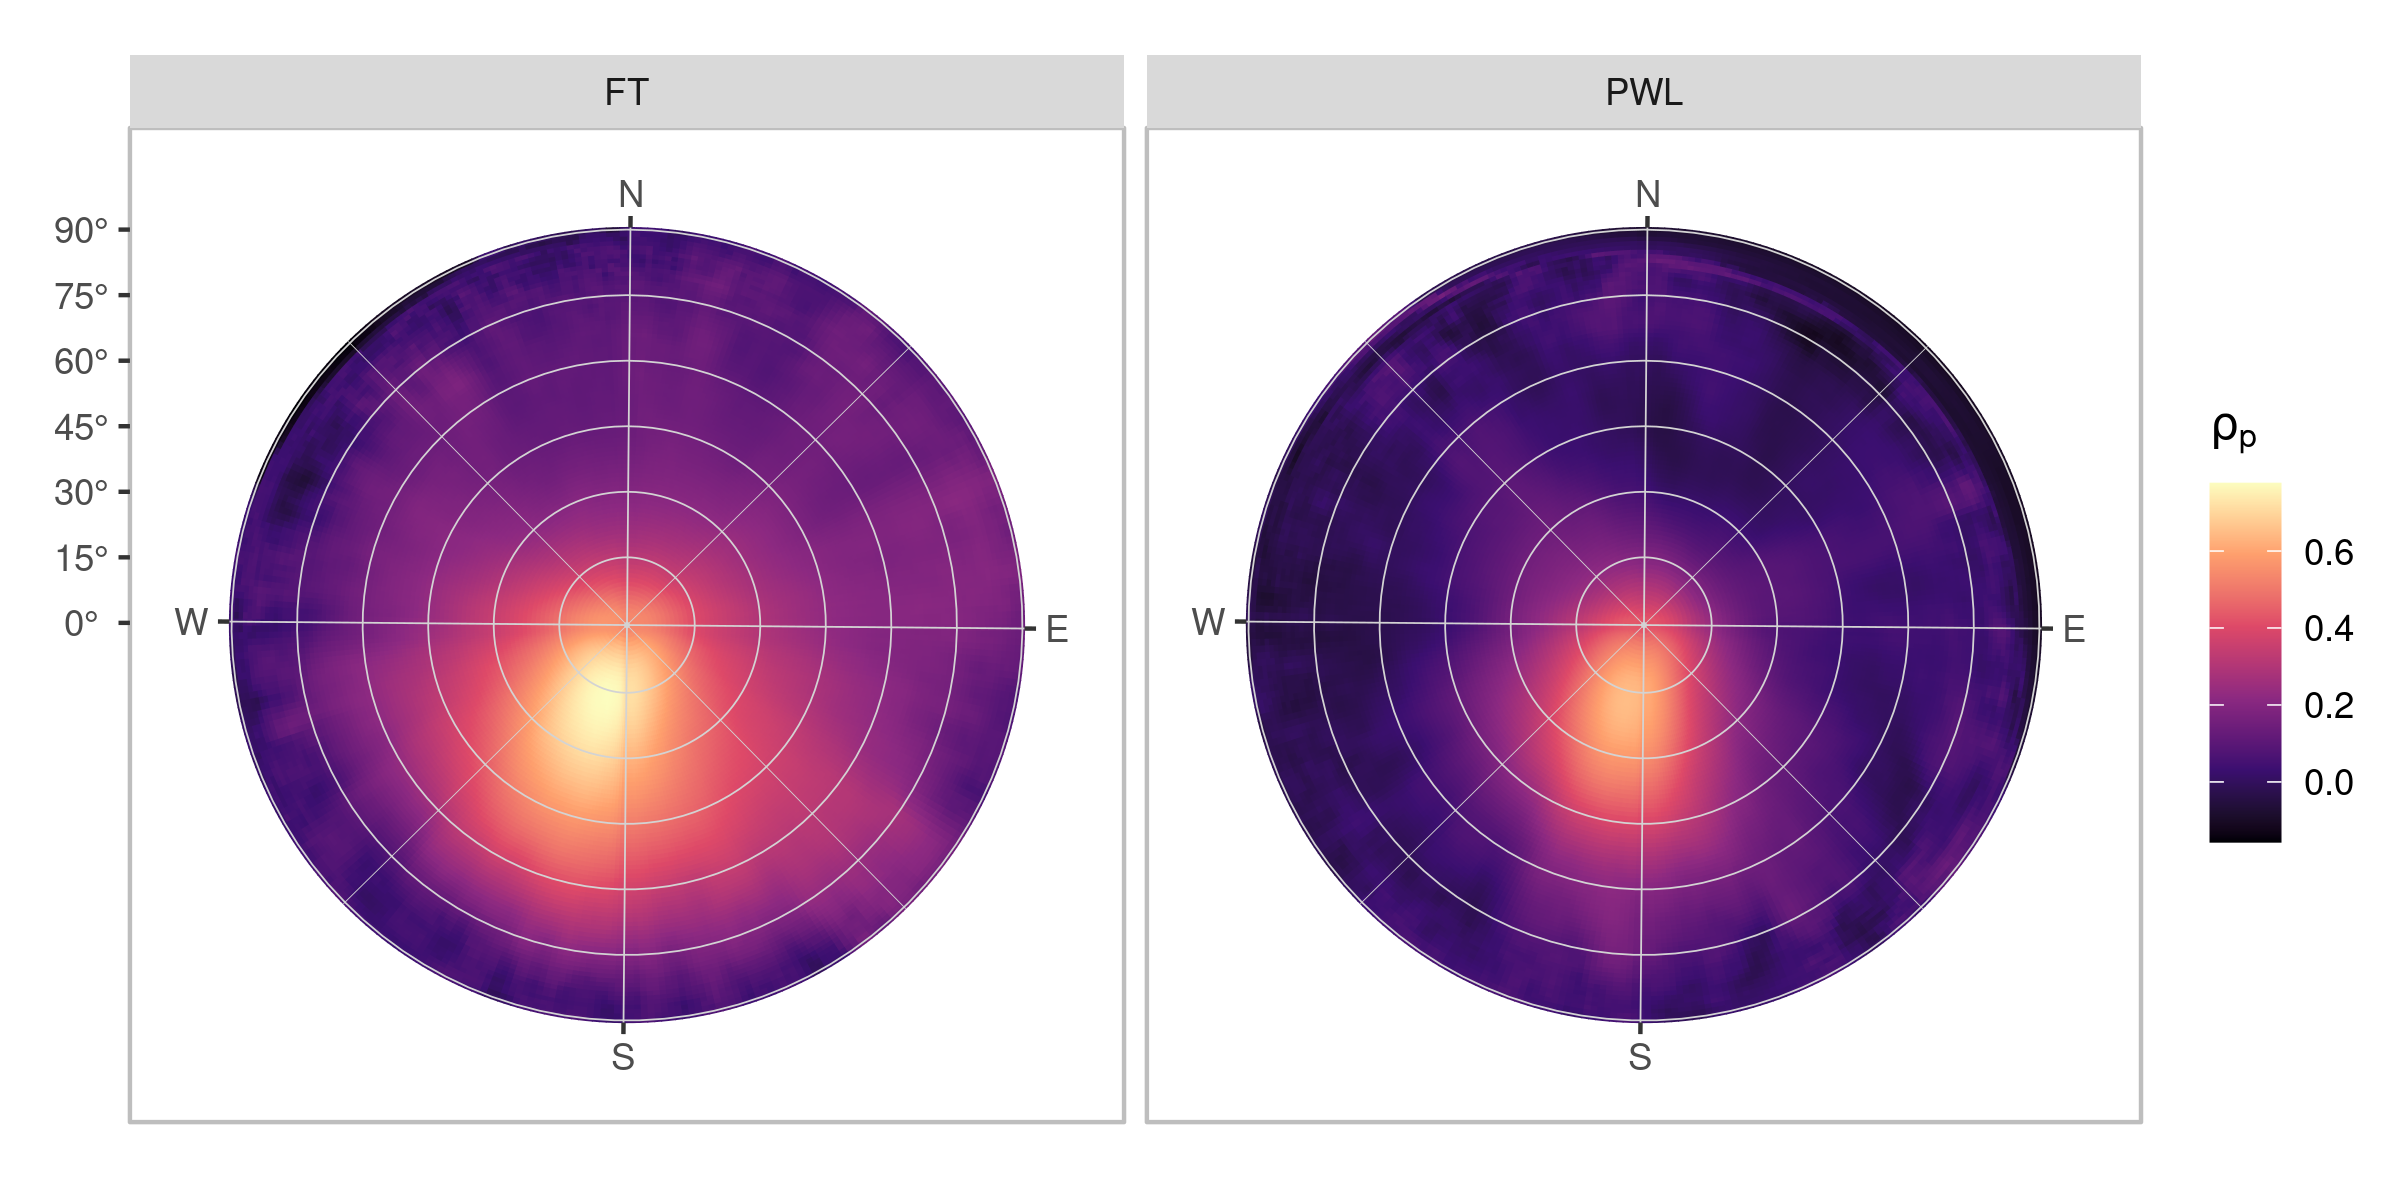
\includegraphics[keepaspectratio]{chapters/03-snow-int-paper/figs/figure7.png}}

}

\caption{\label{fig-hemi-ip-cc}The Pearson Correlation Coefficient
between rasters (0.25 m resolution) of interception efficiency and leaf
contact area (measured on March 13th) for each grid cell across the
study site for each azimuth angles (0°, 1°, \ldots, 359°) and zenith
angles (0°, 1°, \ldots, 90°) for the FT (left) and PWL (right) forest
plots.}

\end{figure}%

The spatial distribution of \(C_p\) measurements, selected based on the
vector corresponding to the azimuth and zenith angles observed to have
the highest correlation with interception efficiency in
Figure~\ref{fig-hemi-ip-cc}, is shown in Figure~\ref{fig-lidar-cc-cp}.
These \(C_p\) measurements generally align with the spatial distribution
of interception efficiency and throughfall
(Figure~\ref{fig-lidar-tf-ip}).

\begin{figure}

\centering{

\pandocbounded{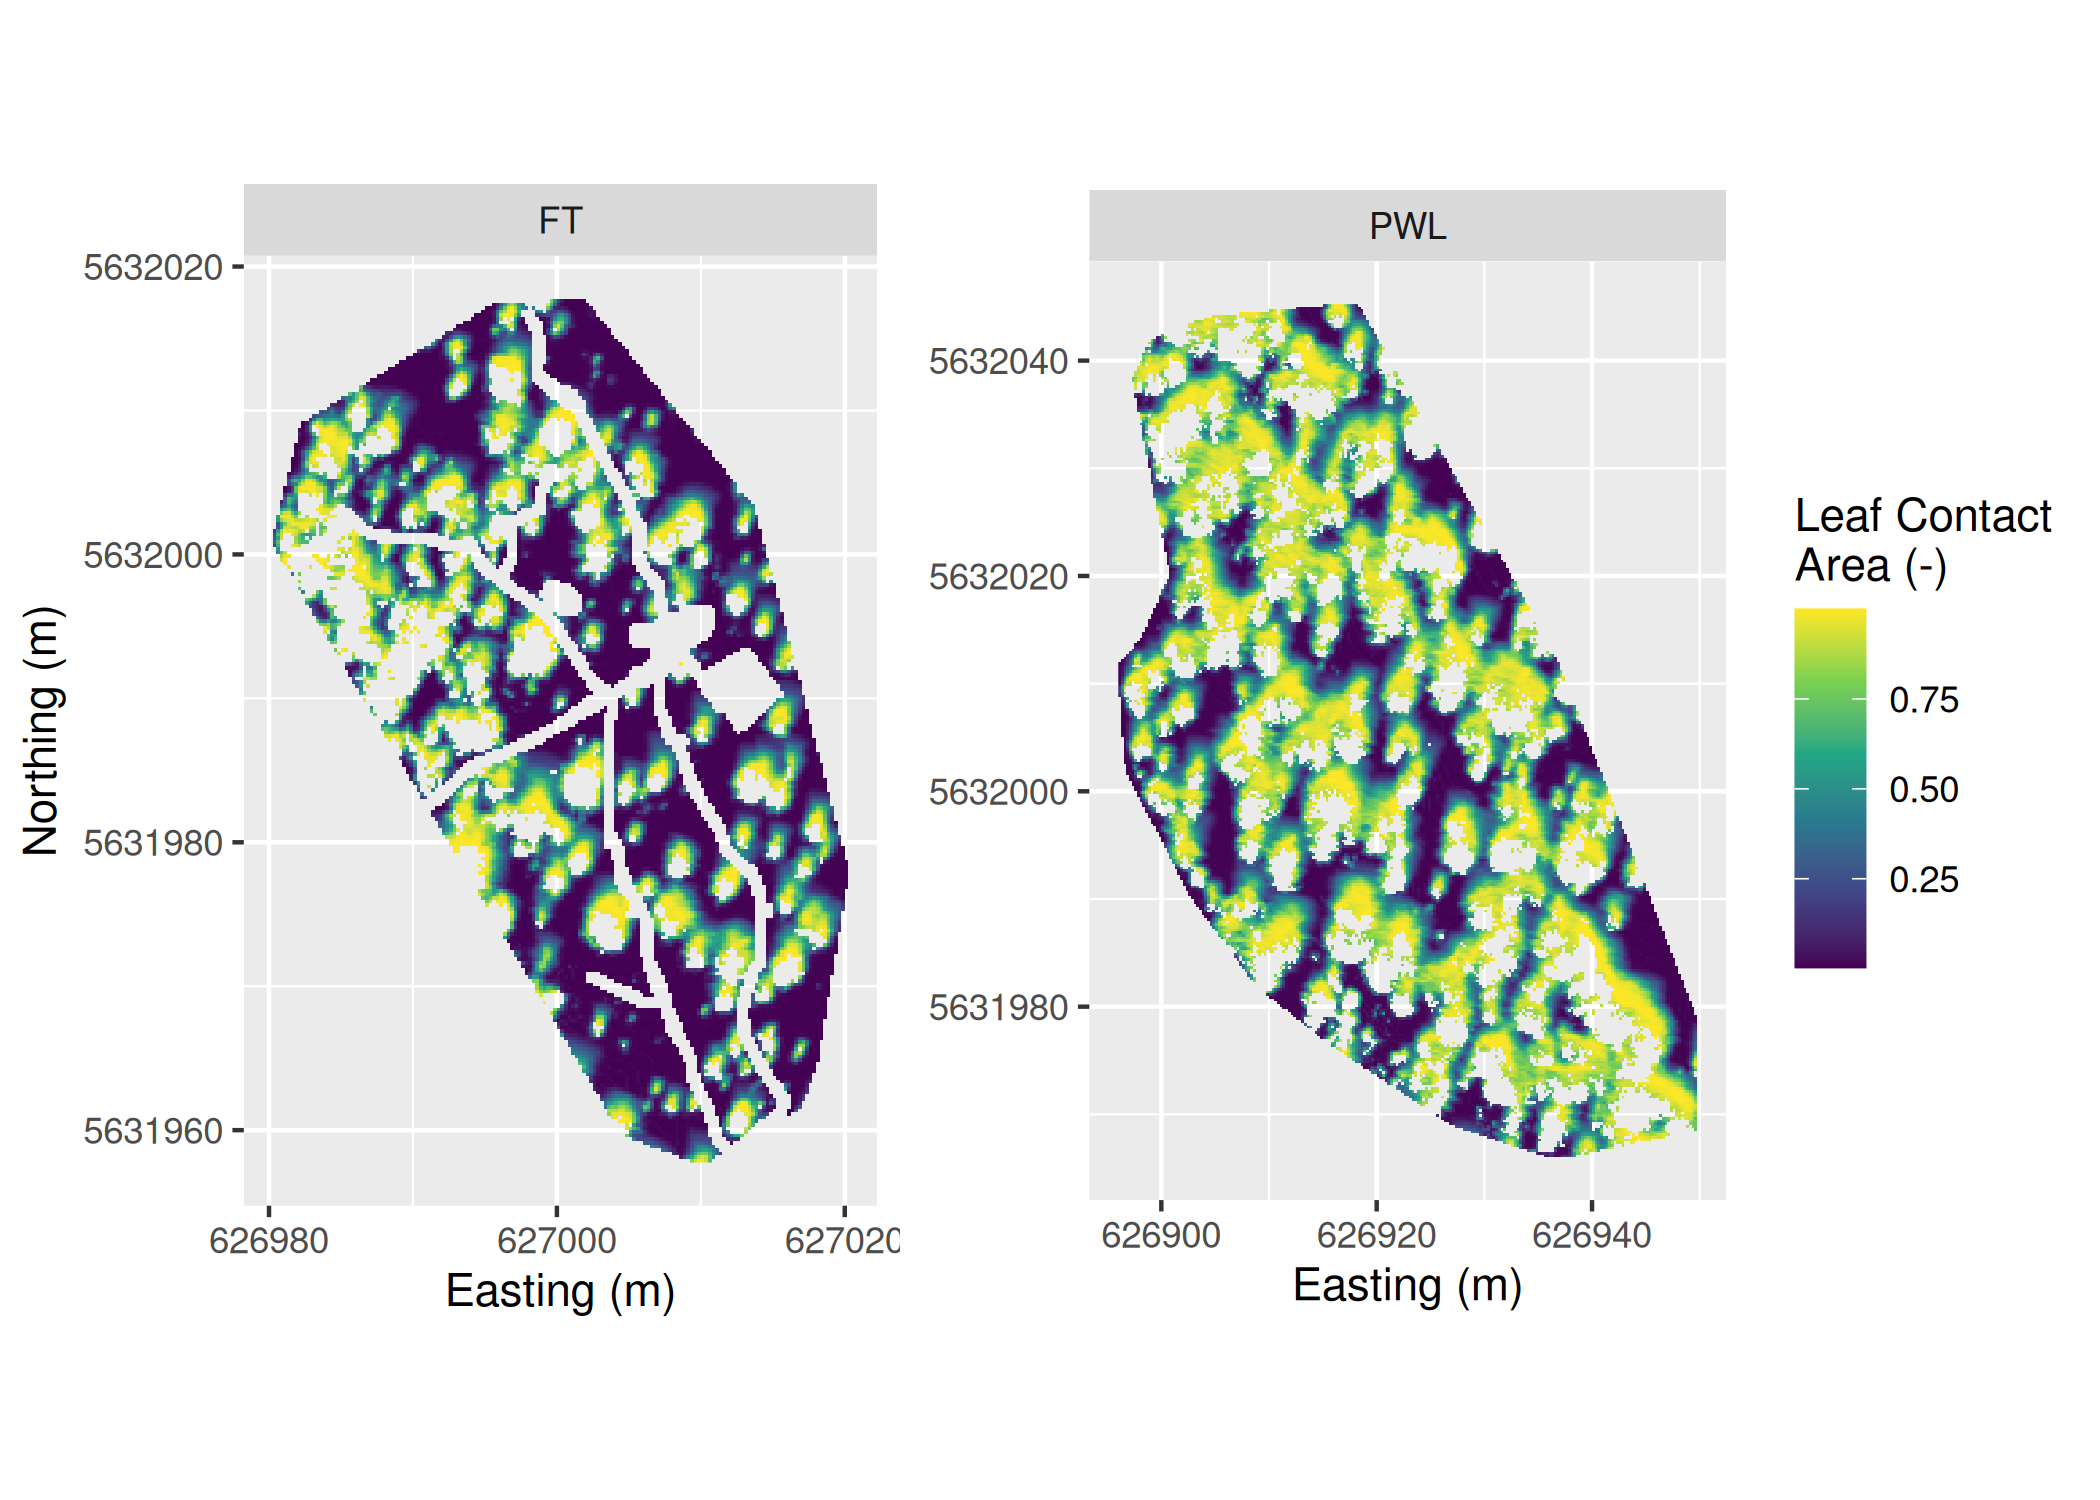
\includegraphics[keepaspectratio]{chapters/03-snow-int-paper/figs/figure8.png}}

}

\caption{\label{fig-lidar-cc-cp}UAV-lidar VoxRS measurements of leaf
contact area measured on March 13\textsuperscript{th} for the PWL and FT
forest plots for zenith angles (PWL = 22°, FT = 21°) and azimuth angles
(PWL = 167°, 178°, \ldots{} 217°; FT = 171°, 172°, \ldots{} 223°).}

\end{figure}%

The correlation between interception efficiency
(Figure~\ref{fig-lidar-tf-ip}) and \(C_p\)
(Figure~\ref{fig-lidar-cc-cp}), resampled to a 5 m grid resolution, was
higher compared to the association with leaf contact angle measured at a
zenith angle of 0° (Figure~\ref{fig-lca-vs-ip}). The stronger
association for the vector-based calculation is hypothesized to stem
from a more accurate representation of the snowfall contact area and
suggests that adjusted \(C_p\) is a useful predictor of interception
efficiency before ablation. An ordinary least squares linear regression
forced through the origin was fit to the observed data points using the
following equation:

\begin{equation}\phantomsection\label{eq-lca-ip}{
  \frac{I}{P} = C_p(C_c, \theta_h) \cdot \alpha
}\end{equation}

where \(\alpha\) is an efficiency constant which determines the fraction
of snowflakes that contact the \(C_p\) elements and are stored in the
canopy (i.e., intercepted) before canopy snow unloading or ablation
processes begin.

\begin{figure}

\centering{

\pandocbounded{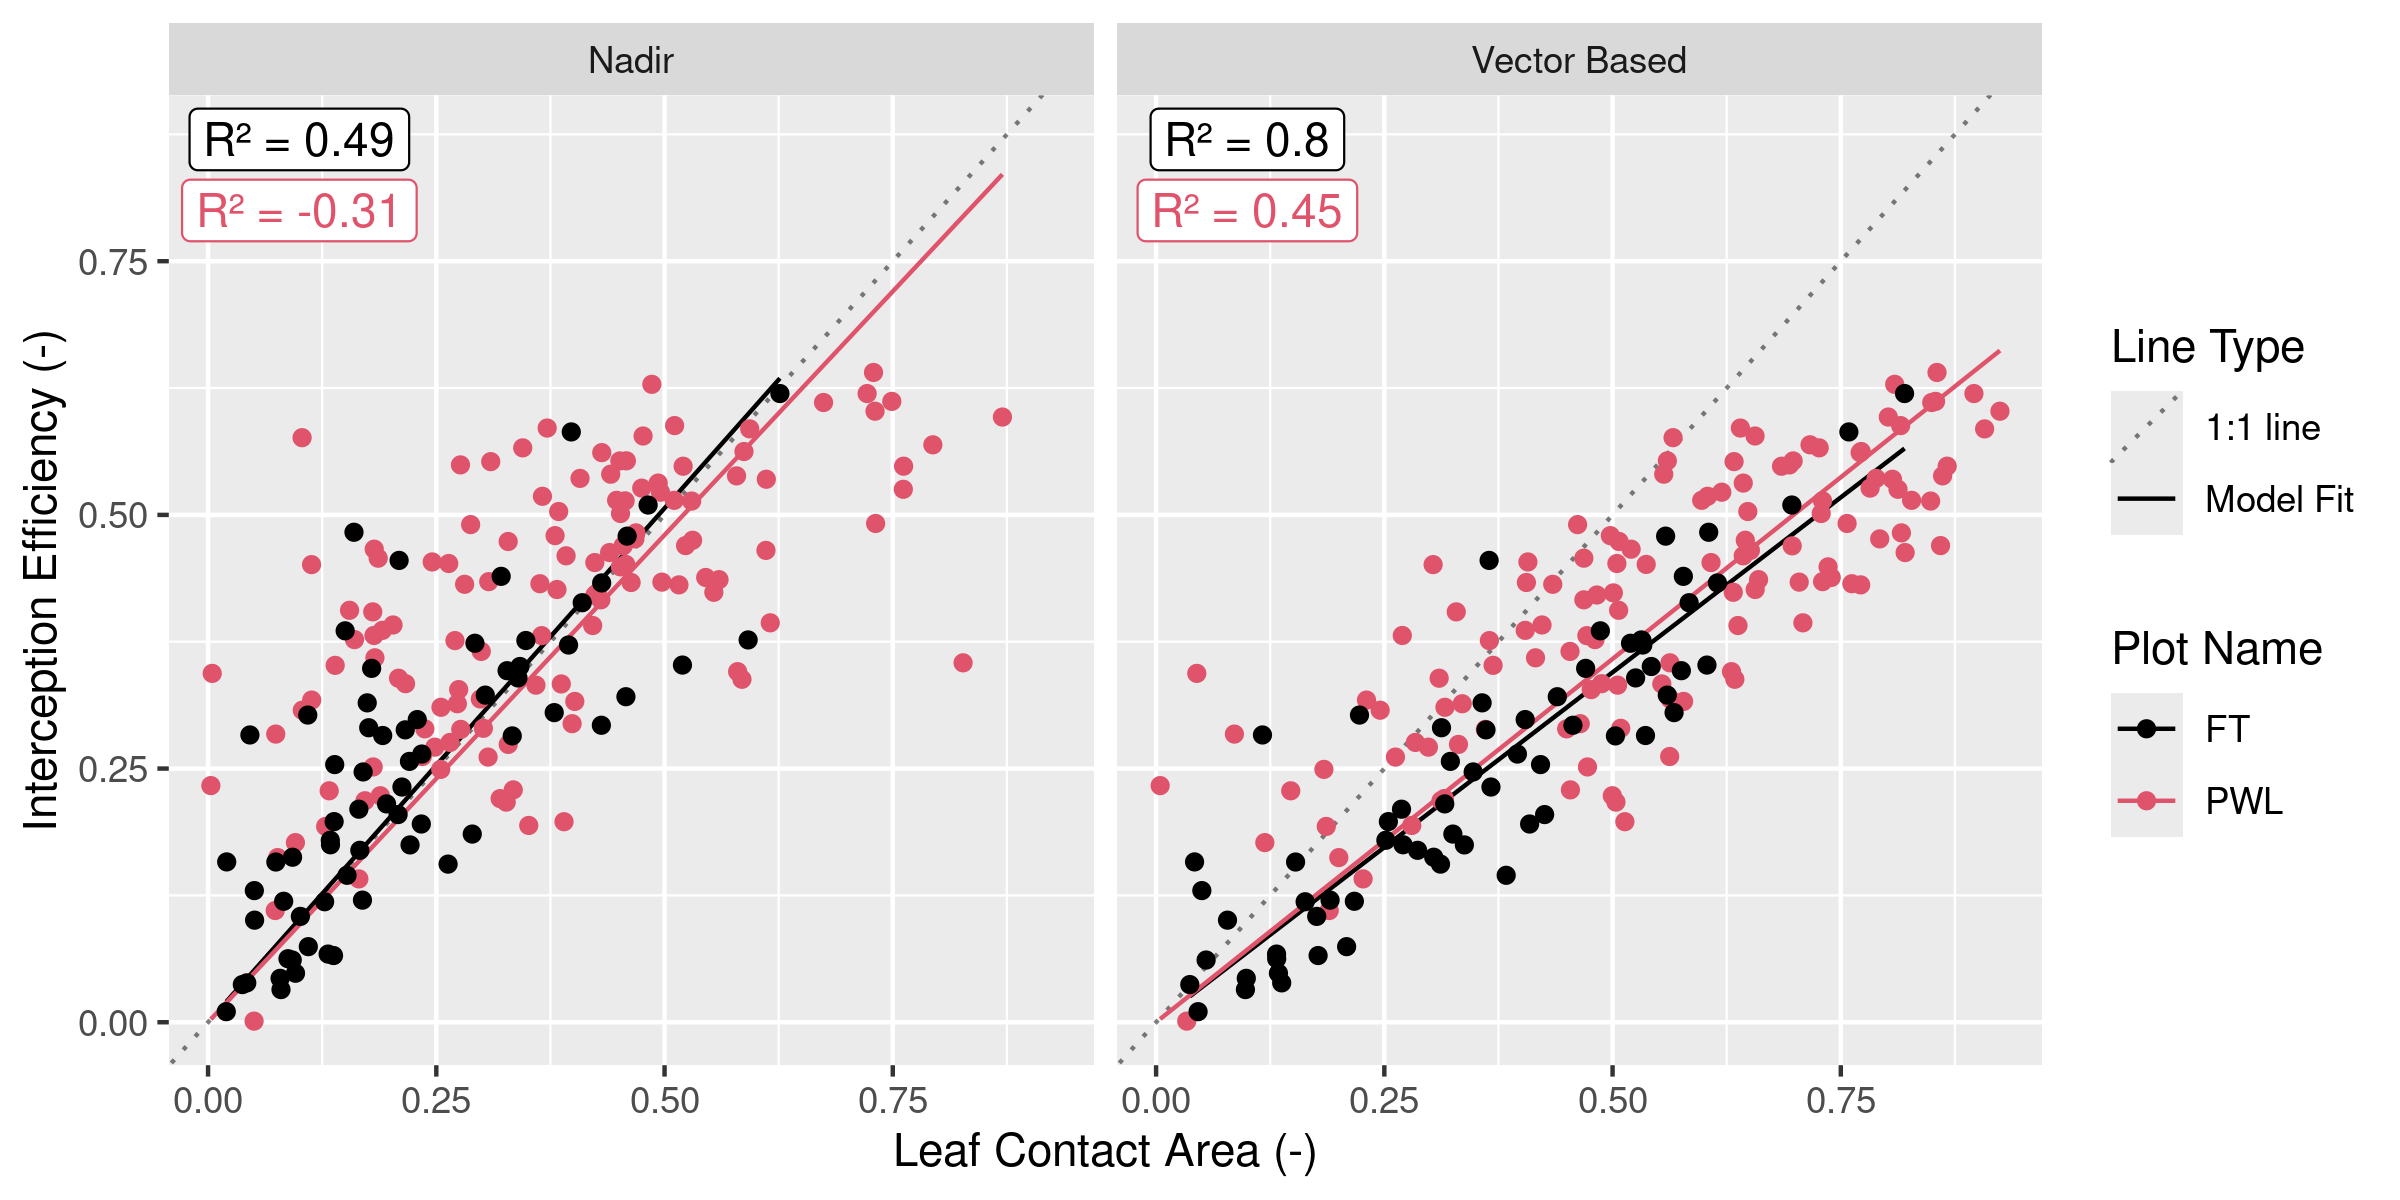
\includegraphics[keepaspectratio]{chapters/03-snow-int-paper/figs/figure9.png}}

}

\caption{\label{fig-lca-vs-ip}Scatter plots showing the relationship
between leaf contact area and interception efficiency rasters resampled
to a 5 m grid cell resolution. The left plot (nadir) shows canopy
coverage and the right plot (Vector Based) shows the leaf contact area
averaged over rasters with zenith angles (PWL = 22°, FT = 21°) and
azimuth angles (PWL = 167°, 178°, \ldots{} 217°; FT = 171°, 172°,
\ldots{} 223°). The solid lines (Model fit) show an ordinary least
squares linear regression forced through the origin and fitted to the
PWL (red) and FT (black) data and the light grey dotted line shows a 1:1
line. The \emph{R}\textsuperscript{2} values for the four different
models are shown in the upper left of each panel calculated following
the methods outlined in Kozak \& Kozak (1995).}

\end{figure}%

For the vector-based model, the relationship between interception
efficiency and \(C_p\) resulted in \emph{R}\textsuperscript{2} values of
0.45 and 0.8 for PWL and FT respectively. Model error statistics show
the vector-based model provided a better prediction of interception
efficiency compared to the nadir canopy coverage measurements
(Table~\ref{tbl-ip-mod-err}). The increase in interception efficiency
with \(C_p\) follows a reduced slope compared to the nadir models with
\(\alpha\) values of 0.72 and 0.69 for the PWL and FT vector-based
models respectively. The reduced slope for the vector-based models may
be due to snowflakes that weaved through and/or bounced off branch
elements in addition to UAV-lidar throughfall measurement uncertainty
which may have been slightly affected by unloading and redistribution.
These processes would have reduced the fraction of snowfall that was
stored in the canopy. Some of the scatter observed in the nadir model
shown in Figure~\ref{fig-lca-vs-ip} may be explained by grid cells
within canopy gaps which observed a greater interception efficiency
compared to the corresponding canopy cover. Conversely, grid cells where
interception efficiency is less than the canopy cover, may be affected
by non-vertical trajectory hydrometeors making their way underneath the
canopy as observed by the reduced interception efficiency on the
windward edges of individual trees in Figure~\ref{fig-lidar-tf-ip}.

\pagebreak

\begin{longtable}[]{@{}
  >{\raggedright\arraybackslash}p{(\linewidth - 12\tabcolsep) * \real{0.1000}}
  >{\raggedright\arraybackslash}p{(\linewidth - 12\tabcolsep) * \real{0.2500}}
  >{\raggedleft\arraybackslash}p{(\linewidth - 12\tabcolsep) * \real{0.1500}}
  >{\raggedleft\arraybackslash}p{(\linewidth - 12\tabcolsep) * \real{0.1500}}
  >{\raggedleft\arraybackslash}p{(\linewidth - 12\tabcolsep) * \real{0.1000}}
  >{\raggedleft\arraybackslash}p{(\linewidth - 12\tabcolsep) * \real{0.1200}}
  >{\raggedleft\arraybackslash}p{(\linewidth - 12\tabcolsep) * \real{0.1300}}@{}}

\caption{\label{tbl-ip-mod-err}Summary of error statistics for the
linear regression models relating leaf contact area to interception
efficiency, presented in Figure~\ref{fig-lca-vs-ip}. The Mean bias is
the difference in the model and observed values, MAE is the mean of the
absolute error, RMS Error is the root mean squared error,
\emph{R}\textsuperscript{2} is the coefficient of determination adjusted
using Equation 10 in Kozak \& Kozak (1995).}

\tabularnewline

\toprule\noalign{}
\begin{minipage}[b]{\linewidth}\raggedright
Plot Name
\end{minipage} & \begin{minipage}[b]{\linewidth}\raggedright
Canopy Calculation
\end{minipage} & \begin{minipage}[b]{\linewidth}\raggedleft
Model Slope (-)
\end{minipage} & \begin{minipage}[b]{\linewidth}\raggedleft
Mean Bias (-)
\end{minipage} & \begin{minipage}[b]{\linewidth}\raggedleft
MAE (-)
\end{minipage} & \begin{minipage}[b]{\linewidth}\raggedleft
RMS Error (-)
\end{minipage} & \begin{minipage}[b]{\linewidth}\raggedleft
\(R^2\)
\end{minipage} \\
\midrule\noalign{}
\endhead
\bottomrule\noalign{}
\endlastfoot
FT & Nadir & 1.01 & 0.024 & 0.072 & 0.101 & 0.49 \\
FT & Vector Based & 0.69 & 0.003 & 0.047 & 0.063 & 0.80 \\
PWL & Nadir & 0.96 & 0.049 & 0.115 & 0.148 & -0.31 \\
PWL & Vector Based & 0.72 & 0.020 & 0.079 & 0.096 & 0.45 \\

\end{longtable}

\subsection{The combined influence of trajectory angle and canopy
density on snow
interception}\label{the-combined-influence-of-trajectory-angle-and-canopy-density-on-snow-interception}

VoxRS measurements of \(C_p\) prior to snowfall on March
13\textsuperscript{th}, increased substantially with simulated
hydrometeor trajectory angle and corresponding simulated wind speed
(Figure~\ref{fig-lca-ht-ws}). The standard deviation in VoxRS measured
\(C_p\), illustrated by the shaded area in Figure~\ref{fig-lca-ht-ws},
exhibits the broad range in values for individual grid cells across each
forest plot. Despite this large scatter, a systematic increase in the
mean \(C_p\) across both forest plots results from a rise in the number
of canopy elements for more horizontal angles, when averaged across each
forest plot, over all azimuth angles (see top left panel
Figure~\ref{fig-lca-ht-ws}). This results in a large rise in \(C_p\)
over relatively common wind speeds. For example, with a wind speed of 1
m s\textsuperscript{-1} and estimated trajectory angle of 48°, \(C_p\)
would increase by 0.31 and 0.28 for the PWL and FT forest plots
respectively (Figure~\ref{fig-lca-ht-ws}). The increase in \(C_p\) from
nadir measured canopy coverage with increasing trajectory angle exhibits
a similar relationship for both forest plots FT and PWL until trajectory
angles reach approximately 60° (see bottom row of
Figure~\ref{fig-lca-ht-ws}). Beyond 60°, the PWL rate of increase slows
as the \(C_p\) approaches 1.0, while the FT plot, which has lower canopy
coverage, continues to rise until around 75° as a \(C_p\) of 1.0 is
approached. \(C_p\) was also quantified across trajectory angles for
both PWL and FT on March 14\textsuperscript{th}, post snowfall, and
showed a negligible increase in \(C_p\) compared to \(C_p\) measured on
March 13\textsuperscript{th} without snow in the canopy.

\begin{figure}

\centering{

\pandocbounded{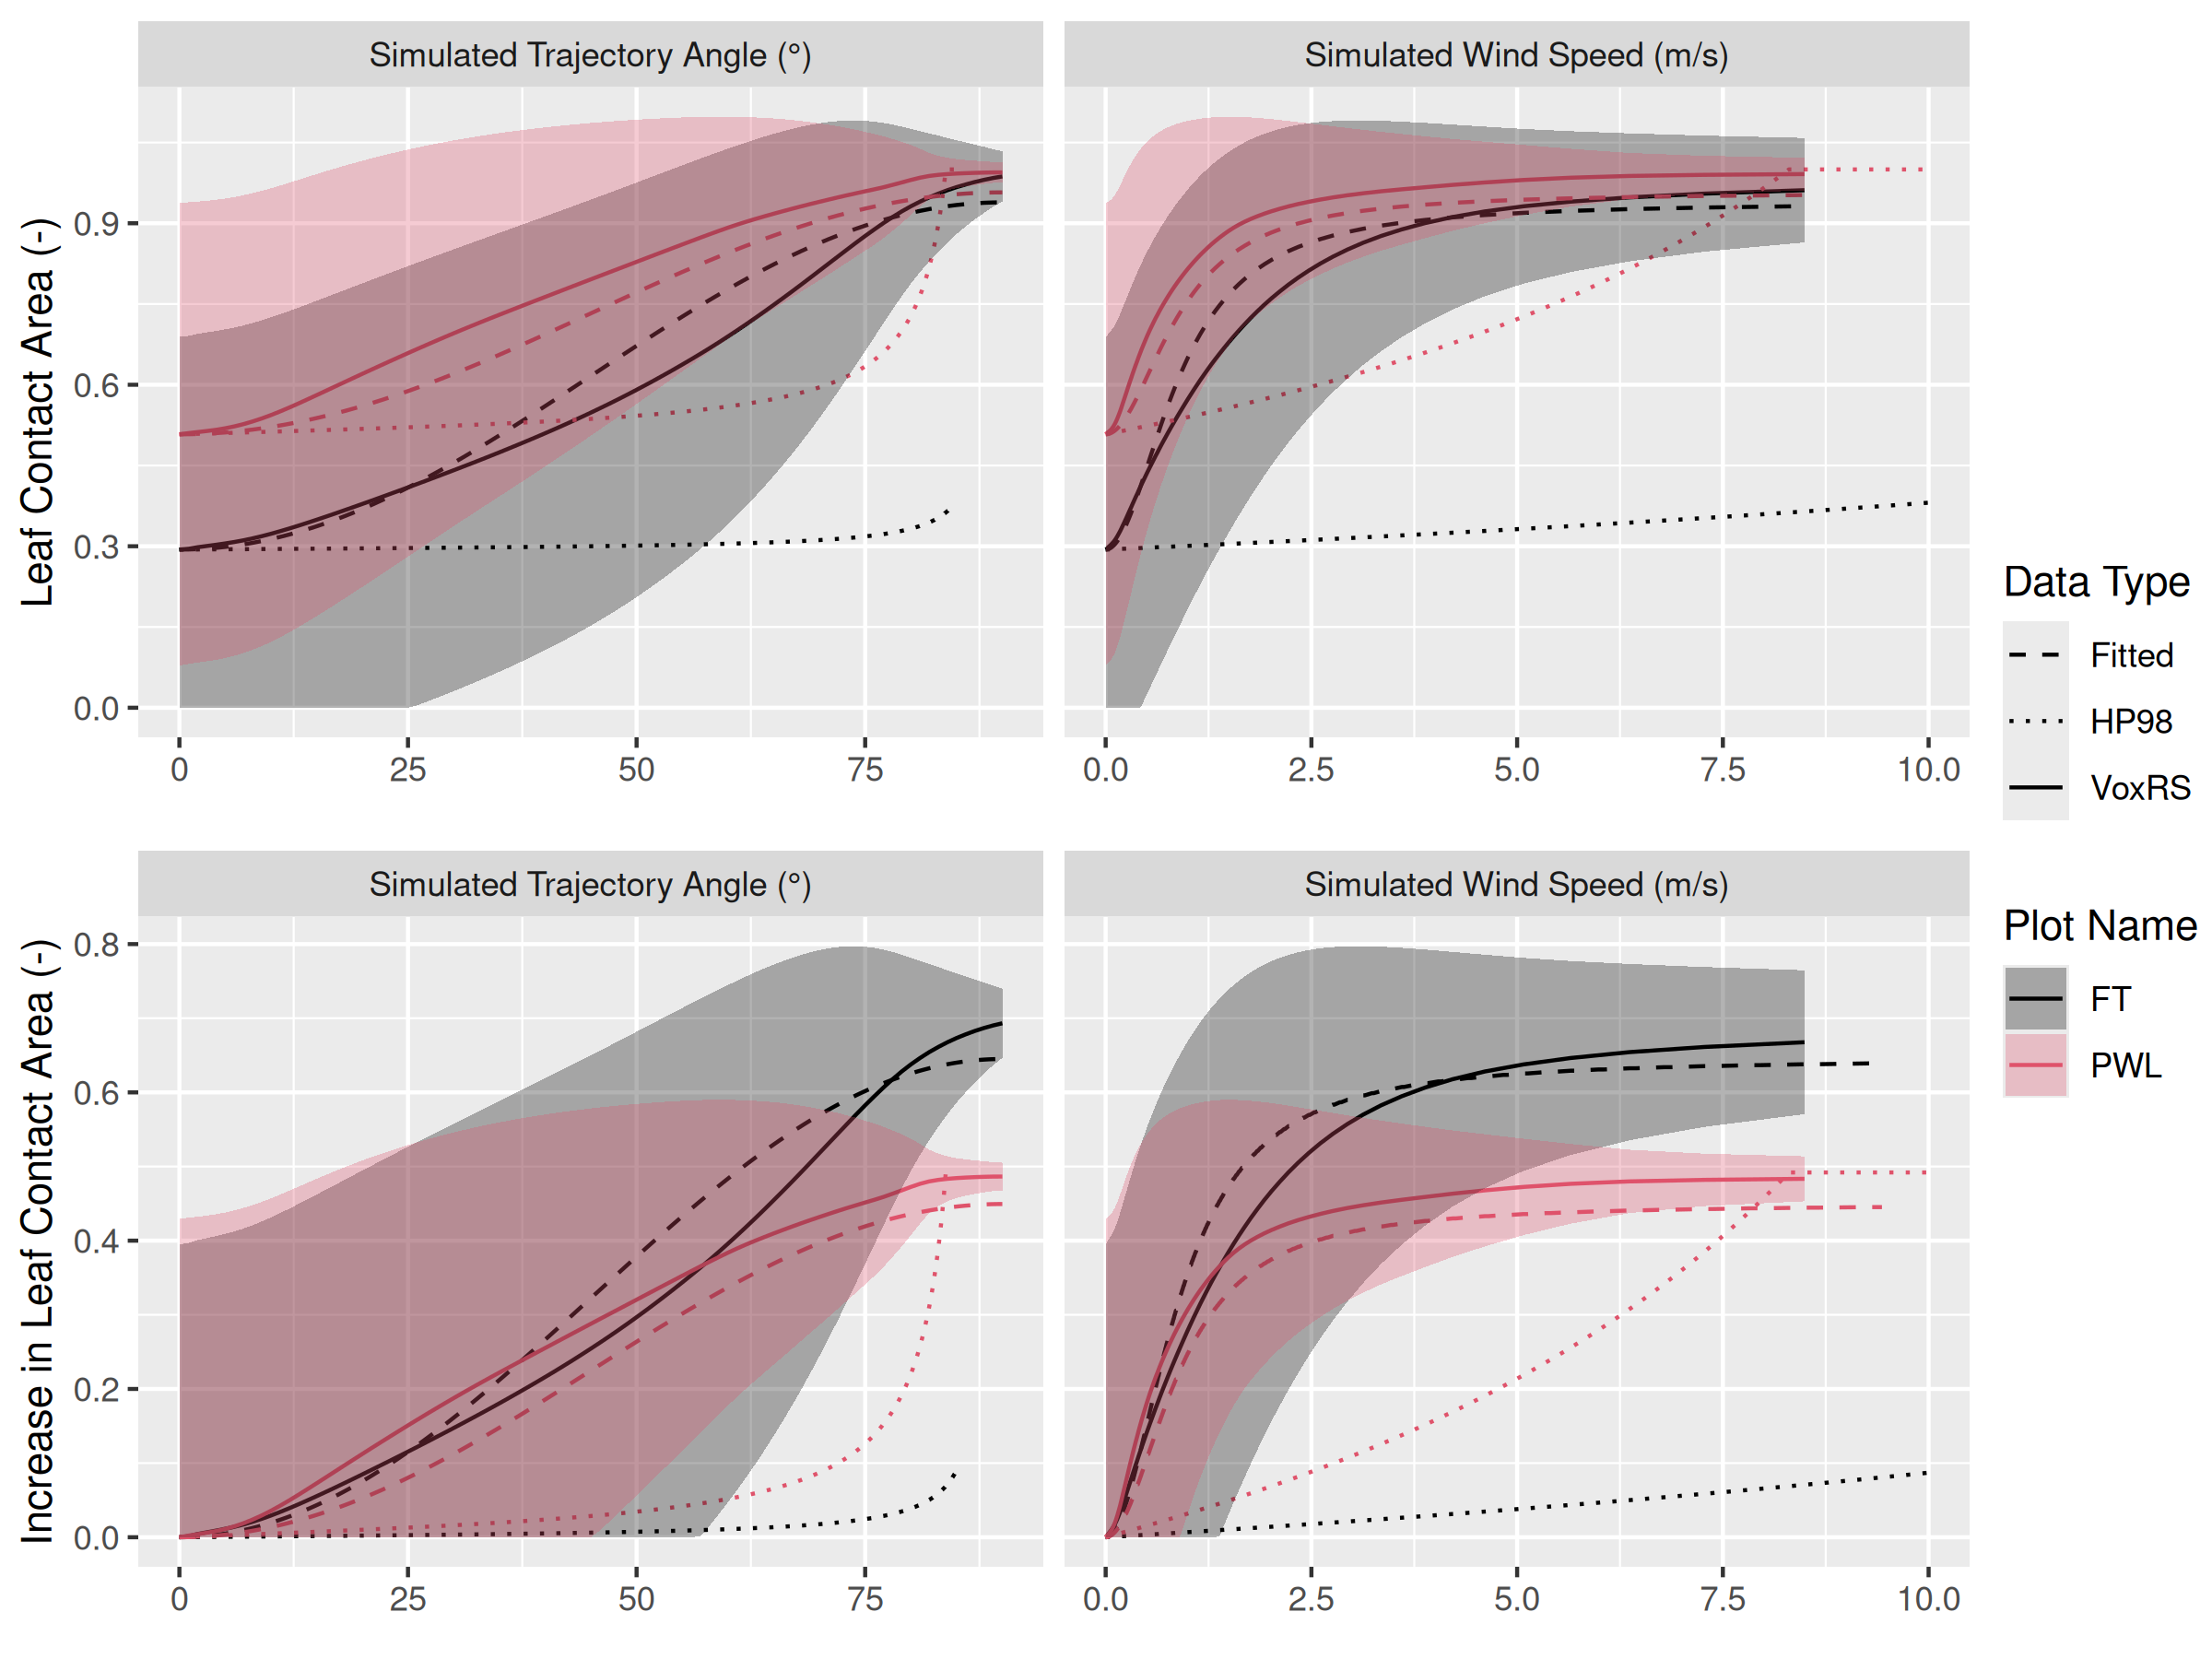
\includegraphics[keepaspectratio]{chapters/03-snow-int-paper/figs/figure10.png}}

}

\caption{\label{fig-lca-ht-ws}Plots showing the relationship between
hydrometeor trajectory angle (left column) and wind speed (right column)
with mean plot-wide snow-leaf contact area, \(C_p\) (top row) and the
increase in mean plot-wide \(C_p\), i.e., \(C_p - C_c\) (bottom row).
The simulated hydrometeor trajectory angle is measured as degrees from
zenith. Simulated wind speed was calculated as a function of hydrometeor
trajectory angle by rearranging Equation~\ref{eq-ta} and an observed
event hydrometeor fall velocity of 0.9 m s\textsuperscript{-1}. The
solid lines (VoxRS) represent the mean \(C_p\) (top row) or increase in
mean \(C_p\) (bottom row) for a single zenith angle observed from VoxRS
across all grid cells for each forest plot and across all azimuth
angles. The shaded area represents one standard deviation above and
below the observed VoxRS mean. The dashed lines (Fitted) represent
predictions from Equation~\ref{eq-lca-ac} (top row) and
Equation~\ref{eq-lca-inc} (bottom row). The dotted lines (HP98)
represent the predictions from Equation 10 in Hedstrom \& Pomeroy
(1998). A forested downwind distance of 100 m was assumed for the HP98
calculation.}

\end{figure}%

A function is proposed here to calculate plot-scale leaf contact area,
\(C_p\) (-):

\begin{equation}\phantomsection\label{eq-lca-ac}{
C_p = C_c + C_{inc}(\theta_h, C_c)
}\end{equation}

where \(C_{inc}\) represents the increase in leaf contact area from
nadir measured canopy coverage (\(C_c\)), and is a function of
\(\theta_h\) and \(C_c\). To estimate \(C_{inc}\) in the absence of
detailed canopy measurements, the following function is proposed:

\begin{equation}\phantomsection\label{eq-lca-inc}{
C_{inc} = (1-C_c)\cdot f(\theta_h)
}\end{equation}

where \(1-C_C\) quantifies the available void space within the canopy
and \(f(\theta_h)\) represents the fraction of that space contributing
to increased leaf contact area. Here, \(f(\theta_h)\) is approximated
as:

\begin{equation}\phantomsection\label{eq-f-theta}{
f(\theta_h) = b \cdot\text{sin}(\theta_h)^2
}\end{equation}

where \(b\) is a fitting coefficient, estimated to be
\textasciitilde0.91 through a non-linear least squares regression fit to
the VoxRS measurements at both FT and PWL. The term
\(\text{sin}(\theta_h)^2\) reflects the relative increase in snow-leaf
contact area, which in turn leads to a proportional decrease in the
canopy void space (\(1-C_c\)). Thus, for \(\theta_h\) of 0°, \(C_p\) is
equal to the canopy cover. In contrast, for \(\theta_h\) close to 90°,
\(C_p\) approaches a value of 1.0. The assumptions of
Equation~\ref{eq-f-theta} include that \(C_c\) represents a measurement
of continuous canopy cover without large open areas many times greater
than the mean canopy height and that snowfall trajectories are linear.

Simulated \(C_p\) using Equation~\ref{eq-lca-ac} is shown in the dashed
lines in the top row of Figure~\ref{fig-lca-ht-ws} and follows the
VoxRS-measured mean \(C_p\) closely. Model error statistics demonstrate
that Equation~\ref{eq-lca-inc} performed well, with a mean bias and RMSE
of -0.05 (-) and 0.05 (-) for PWL, and 0.03 (-) and 0.05 (-) for FT
respectively (Table~\ref{tbl-lca-mod-err}). In contrast, the Hedstrom \&
Pomeroy (1998) method produced significantly less accurate estimates of
\(C_p\), with a mean bias and RMSE of -0.2 (-) and 0.23 (-) for PWL, and
-0.26 (-) and 0.32 (-) for FT respectively
(Table~\ref{tbl-lca-mod-err}).

\begin{longtable}[]{@{}
  >{\raggedright\arraybackslash}p{(\linewidth - 10\tabcolsep) * \real{0.1500}}
  >{\raggedright\arraybackslash}p{(\linewidth - 10\tabcolsep) * \real{0.1700}}
  >{\raggedleft\arraybackslash}p{(\linewidth - 10\tabcolsep) * \real{0.1700}}
  >{\raggedleft\arraybackslash}p{(\linewidth - 10\tabcolsep) * \real{0.1500}}
  >{\raggedleft\arraybackslash}p{(\linewidth - 10\tabcolsep) * \real{0.2000}}
  >{\raggedleft\arraybackslash}p{(\linewidth - 10\tabcolsep) * \real{0.1700}}@{}}

\caption{\label{tbl-lca-mod-err}Model error statistics calculated for
the prediction of leaf contact area from trajectory angle using
Equation~\ref{eq-lca-inc} and Equation 10 from Hedstrom \& Pomeroy
(1998) (HP98) for the PWL and FT forest plots. Mean bias is the
difference in the model and observed values, MAE is the mean of the
absolute error, RMS Error is the root mean squared error and
\emph{R}\textsuperscript{2} is the coefficient of determination. The
units for all metrics are dimensionless. A forested downwind distance of
100 m was used for the HP98 calculation.}

\tabularnewline

\toprule\noalign{}
\begin{minipage}[b]{\linewidth}\raggedright
Model
\end{minipage} & \begin{minipage}[b]{\linewidth}\raggedright
Plot Name
\end{minipage} & \begin{minipage}[b]{\linewidth}\raggedleft
Mean Bias (-)
\end{minipage} & \begin{minipage}[b]{\linewidth}\raggedleft
MAE (-)
\end{minipage} & \begin{minipage}[b]{\linewidth}\raggedleft
RMS Error (-)
\end{minipage} & \begin{minipage}[b]{\linewidth}\raggedleft
\(R^2\)
\end{minipage} \\
\midrule\noalign{}
\endhead
\bottomrule\noalign{}
\endlastfoot
HP98 & FT & -0.26 & 0.26 & 0.32 & -0.97 \\
HP98 & PWL & -0.20 & 0.20 & 0.23 & -0.96 \\
Eq. 10 & FT & 0.03 & 0.04 & 0.05 & 0.95 \\
Eq. 10 & PWL & -0.05 & 0.05 & 0.05 & 0.90 \\

\end{longtable}

\subsection{Throughfall model
performance}\label{throughfall-model-performance}

The performance of the interception efficiency
(Equation~\ref{eq-lca-ip}) and leaf contact area
(Equation~\ref{eq-lca-ac}) parameterisations in estimating event
throughfall was assessed against UAV-lidar measurements of throughfall
at the plot scale for the March 13--14\textsuperscript{th} snowfall
event. In this assessment, the hydrometeor trajectory angle was
approximated using Equation~\ref{eq-ta} combined with the mean event
wind speed at one-third the mean canopy height (estimated from
Equation~\ref{eq-cionco} and the observed wind speed at FT station) and
hydrometeor terminal velocity (measured at PWL station). Leaf contact
area was then estimated using Equation~\ref{eq-lca-ac} for the PWL and
FT plots, incorporating the approximated hydrometeor trajectory angle
and observed canopy cover (\(C_c\)) from the VoxRS dataset. Interception
efficiency was calculated using Equation~\ref{eq-lca-ip} with the
estimated leaf contact area from Equation~\ref{eq-lca-ac} and
accumulated snowfall measured at PWL station for the event. An
\(\alpha\) value, used in Equation~\ref{eq-lca-ip}, of 0.978 (-) was
found through calibration which provided the best fit between observed
and simulated interception efficiency at the plot scale for both FT and
PWL.

The new vector-based parameterisation closely matched the UAV-lidar
measurements of throughfall (Figure~\ref{fig-event-tf}). Modelled
throughfall from the vector-based model was 17.2 mm compared to the
measured throughfall of 16.6 mm for PWL. For FT, the vector-based
modelled throughfall was 21.5 mm, while the measured values where 22.1
mm. The vector-based model shows a lower mean bias of -0.6 mm for PWL
and 0.6 mm for FT, in contrast to the nadir-based model, which
overestimated throughfall for both plots (Table~\ref{tbl-vb-plot-err}).
This overestimation arose from the nadir-based model's approximation of
leaf contact area from canopy coverage measurements (without adjustment
via Equation~\ref{eq-lca-ac}), which yielded a reduced estimated contact
area and consequently underestimated canopy snow interception.

\begin{figure}

\centering{

\pandocbounded{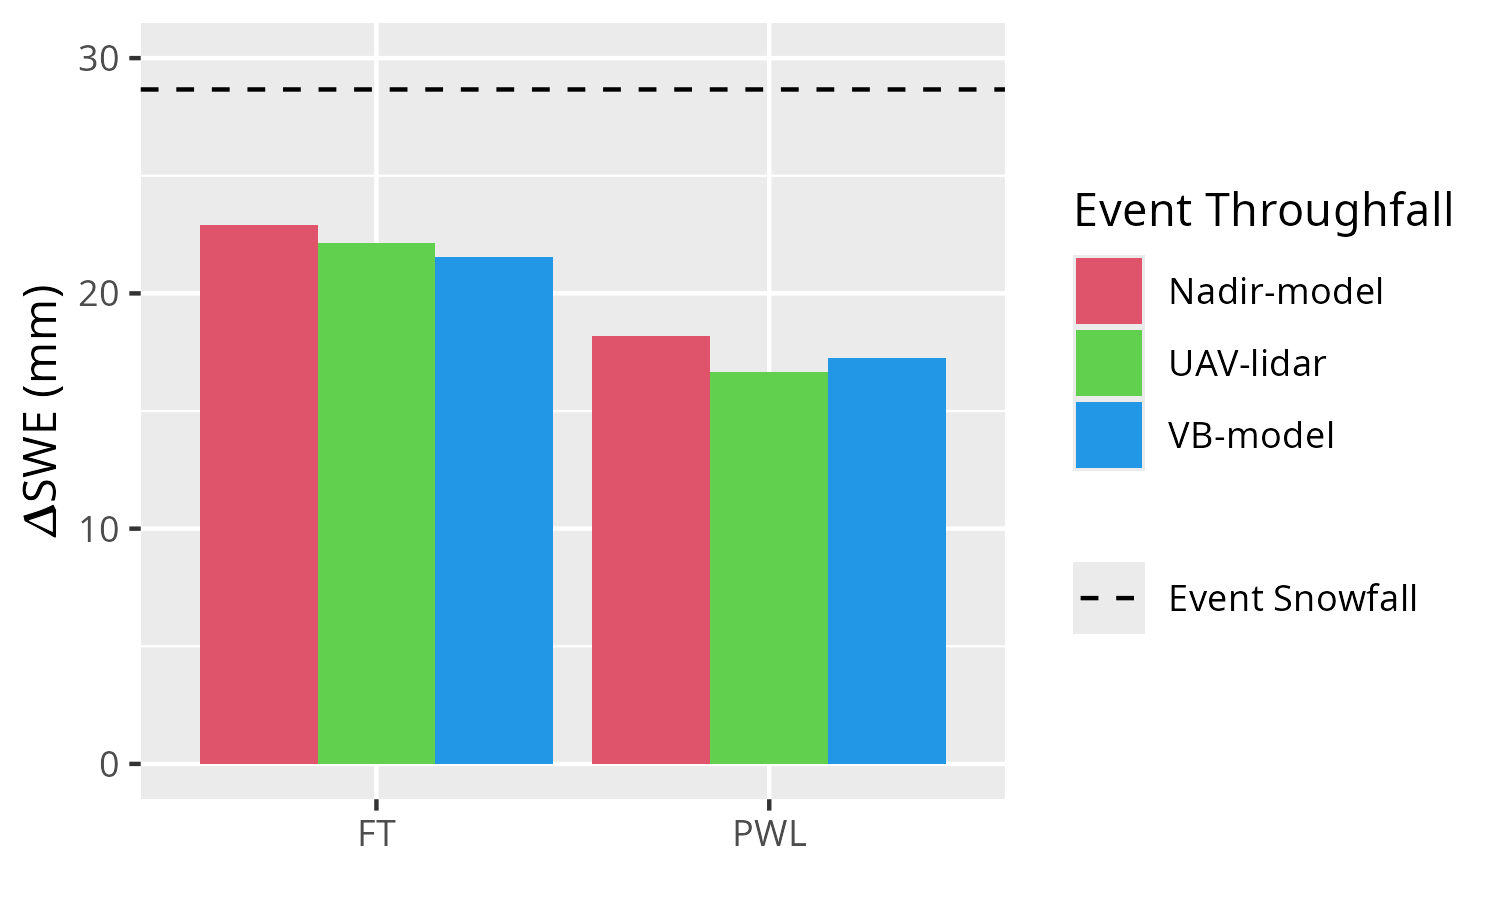
\includegraphics[keepaspectratio]{chapters/03-snow-int-paper/figs/figure11.png}}

}

\caption{\label{fig-event-tf}Bar chart comparing the observed and
modelled mean change in throughfall (ΔSWE, mm) over the March
13-14\textsuperscript{th} snowfall event averaged over forest plots FT
and PWL. The `Nadir-model' calculated interception efficiency as a
function of canopy coverage and the Vector-based `VB-model' used
Equation~\ref{eq-lca-ip} with \(C_p\) adjusted for trajectory angle.
`UAV-lidar' corresponds to throughfall calculated using
Equation~\ref{eq-swe-tf} incorporating UAV-lidar snow depth and snow
density from in-situ snow pits. The black horizontal dashed line shows
the accumulated SWE (mm) over the snowfall event to the PWL station open
clearing.}

\end{figure}%

\pagebreak

\begin{longtable}[]{@{}
  >{\raggedright\arraybackslash}p{(\linewidth - 14\tabcolsep) * \real{0.1200}}
  >{\raggedright\arraybackslash}p{(\linewidth - 14\tabcolsep) * \real{0.1200}}
  >{\raggedright\arraybackslash}p{(\linewidth - 14\tabcolsep) * \real{0.1200}}
  >{\raggedright\arraybackslash}p{(\linewidth - 14\tabcolsep) * \real{0.1000}}
  >{\raggedleft\arraybackslash}p{(\linewidth - 14\tabcolsep) * \real{0.1000}}
  >{\raggedleft\arraybackslash}p{(\linewidth - 14\tabcolsep) * \real{0.1000}}
  >{\raggedleft\arraybackslash}p{(\linewidth - 14\tabcolsep) * \real{0.1000}}
  >{\raggedleft\arraybackslash}p{(\linewidth - 14\tabcolsep) * \real{0.1000}}@{}}

\caption{\label{tbl-vb-plot-err}Model error statistics for model
estimates of snow interception efficiency (I/P) and throughfall (TF)
compared to measurements of I/P and TF using UAV-lidar averaged over the
FT and PWL forest plots. Units for I/P are (-) and TF are (mm). The
vector-based model utilized Equation~\ref{eq-lca-ip} with \(C_p\)
adjusted for trajectory angle. The nadir model also utilized
Equation~\ref{eq-lca-ip} but was not adjusted for trajectory angle and
thus \(C_c\) was used instead of \(C_p\). The `Obs. Value' column
contains measurements from UAV-lidar while the `Mod. Value' column
contains the modelled values. The mean bias was calculated as observed
minus modelled and percent error is the percent error between predicted
and observed values.}

\tabularnewline

\toprule\noalign{}
\begin{minipage}[b]{\linewidth}\raggedright
Plot
\end{minipage} & \begin{minipage}[b]{\linewidth}\raggedright
Model Type
\end{minipage} & \begin{minipage}[b]{\linewidth}\raggedright
Value Name
\end{minipage} & \begin{minipage}[b]{\linewidth}\raggedright
Units
\end{minipage} & \begin{minipage}[b]{\linewidth}\raggedleft
Obs. Value
\end{minipage} & \begin{minipage}[b]{\linewidth}\raggedleft
Mod. Value
\end{minipage} & \begin{minipage}[b]{\linewidth}\raggedleft
Mean Bias
\end{minipage} & \begin{minipage}[b]{\linewidth}\raggedleft
Perc. Error
\end{minipage} \\
\midrule\noalign{}
\endhead
\bottomrule\noalign{}
\endlastfoot
FT & VB-model & I/P & - & 0.23 & 0.25 & -0.02 & -9.01 \\
FT & Nadir-model & I/P & - & 0.23 & 0.20 & 0.03 & 12.10 \\
FT & VB-model & TF & mm & 22.12 & 21.53 & 0.59 & 2.67 \\
FT & Nadir-model & TF & mm & 22.12 & 22.91 & -0.79 & -3.58 \\
PWL & VB-model & I/P & - & 0.42 & 0.40 & 0.02 & 4.91 \\
PWL & Nadir-model & I/P & - & 0.42 & 0.37 & 0.05 & 12.95 \\
PWL & VB-model & TF & mm & 16.64 & 17.24 & -0.59 & -3.55 \\
PWL & Nadir-model & TF & mm & 16.64 & 18.20 & -1.56 & -9.35 \\

\end{longtable}

\section{Discussion}\label{discussion-1}

The point scale observations presented in Figure~\ref{fig-scl-ip-bins}
indicate that air temperature had little influence on initial
interception efficiency during periods where melt and unloading of snow
were less likely. This finding aligns with Storck et al. (2002), who
observed that variations in air temperature did not significantly affect
initial interception efficiency. While other studies have reported both
positive (Andreadis et al., 2009; Katsushima et al., 2023; Roth \&
Nolin, 2019) and negative (Hedstrom \& Pomeroy, 1998; Schmidt \& Gluns,
1991) relationships between air temperature and snow interception, the
limited association observed here may be explained by competing
temperature-dependent processes. Warmer temperatures simultaneously
increase branch flexibility, reducing \(C_p\) (Schmidt \& Gluns, 1991;
Schmidt \& Pomeroy, 1990) and enhance snow cohesion and adhesion,
increasing interception efficiency (Katsushima et al., 2023; Kobayashi,
1987; Pfister \& Schneebeli, 1999).

Initial interception efficiency was found to increase with wind speed at
two locations which were sheltered from the predominant wind direction
(Figure~\ref{fig-scl-ip-bins}). This is hypothesized to be due to an
increase in \(C_p\) associated with non-vertical hydrometeor
trajectories, as demonstrated by observations during a wind-driven
snowfall event (Figure~\ref{fig-lidar-tf-ip}) and analysis of canopy
density data (Figure~\ref{fig-lca-ht-ws}). These findings are also
consistent with observations by Schmidt \& Troendle (1989) who observed
a slight increase in snowfall interception with increasing wind speeds
up to 6 m s\textsuperscript{-1}, Staines \& Pomeroy (2023) who observed
reduced canopy transmittance with increasing angle from zenith, and
studies of rainfall interception by Herwitz \& Slye (1995) and Van Stan
et al. (2011).

The slight increase in interception efficiency for smaller canopy snow
loads and decline for larger canopy snow loads is attributed to the
influence of canopy snow load on \(C_p\) (Figure~\ref{fig-scl-ip-bins}).
Whilst small, this effect is consistent with the theory proposed by
Satterlund \& Haupt (1967) that interception efficiency increases as the
canopy fills with snow bridging gaps in the canopy, while later
declining due to branch bending and decreased canopy cover. However, at
the plot-scale, Staines \& Pomeroy (2023) showed that these two
processes may partially compensate for each other as \(C_p\) increases
for closed canopies, as new snow bridges form in the canopy, but
decreases in partially open canopy due to branch bending (i.e., Fig. 2
in Schmidt \& Gluns, 1991). Still, the increase in \(C_p\) resulting
from snow load in Staines \& Pomeroy (2023) was small compared to the
substantial rise in \(C_p\) due to trajectory angle presented in their
study; which corroborates with the plot-scale observations of \(C_p\) in
this study (Figure~\ref{fig-lca-ht-ws}). Additional observations by
Watanabe \& Ozeki (1964), Calder (1990), and Storck et al. (2002)
support the findings in Figure~\ref{fig-scl-w-sf} showing a linear
increase in canopy snow load with increasing snowfall. Further evidence
in support of the relatively small influence of canopy snow load on
\(C_p\), is provided by Lundquist et al. (2021) who reported improved
simulation of subcanopy snow accumulation without the use of a maximum
canopy snow load, when linked with a comprehensive canopy snow ablation
routine. The low sensitivity to canopy snow load found here may result
from reduced inclusion of ablation processes in our measurements,
limited influence of snow load on \(C_p\) at this site, and/or the
compensatory effects described by Satterlund \& Haupt (1967).

The limited influence of air temperature and canopy snow load on initial
interception reported here differs from the theories underpinning
existing snow interception parameterisations (Andreadis et al., 2009;
Hedstrom \& Pomeroy, 1998; Moeser et al., 2015b; Satterlund \& Haupt,
1967). Cebulski \& Pomeroy (2025a) note studies that have identified a
relationship between air temperature and/or snow load and interception
efficiency (Katsushima et al., 2023; Roth \& Nolin, 2019; Schmidt \&
Gluns, 1991) did not specifically examine initial interception prior to
canopy snow ablation. In addition, since a maximum canopy snow load was
not observed in this study, the air temperature dependent canopy snow
load capacities included in the Hedstrom \& Pomeroy (1998) and Andreadis
et al. (2009) models were not applicable. Since canopy snow ablation is
strongly correlated with air temperature and snow load (Ellis et al.,
2010; Floyd, 2012; Hedstrom \& Pomeroy, 1998; Roesch et al., 2001) some
of the previously observed relationships related to these variables may
be explained by changes in ablation rather than initial interception.
The coupling of ablation processes within existing models may contribute
to overestimates of throughfall and canopy snow unloading when combined
with other canopy snow ablation parameterisations due to `double
counting' (Cebulski \& Pomeroy, 2025a).

To address these issues, a new vector-based snow interception
parameterisation is presented (Equation~\ref{eq-lca-ip}) which
calculates initial interception efficiency as a function of \(C_p\) and
an efficiency constant, \(\alpha\). This new parameterisation allows for
canopy snow loading processes to be isolated from canopy snow ablation
processes and is consistent with current rainfall interception theory
(Valante et al., 1997; Zhong et al., 2022). Equation~\ref{eq-lca-ip}
differs only slightly from the original Hedstrom \& Pomeroy (1998)
parameterisation (see Equation 6 in Hedstrom \& Pomeroy 1998), in that
it does not calculate interception efficiency as a function of canopy
snow load and from the Storck et al. (2002) parameterisation who found
interception efficiency to be constant. Further research is needed to
explore how processes such as the increased cohesion and adhesion of
snowfall to the canopy at warm temperatures, as observed by Kobayashi
(1987), Pfister \& Schneebeli (1999), as well as hydrometeor velocity,
particle size, and shape suggested by (Katsushima et al., 2023), may
influence the \(\alpha\) parameter, although these effects were not
observed in this study. Since Equation~\ref{eq-lca-ip} intentionally
excludes processes attributed to canopy snow ablation that were
previously included in earlier snow interception models, these ablation
processes must be incorporated in canopy snow ablation parameterisations
to fully represent the canopy snow mass balance.

The exponential relationship proposed by Hedstrom \& Pomeroy (1998) to
scale \(C_p\) with wind speed failed to reproduce the observations
presented in Figure~\ref{fig-lca-ht-ws}. Instead, plot-wide \(C_p\) was
found to increase as function of hydrometeor trajectory angle and canopy
cover. However, the large scatter in \(C_p\) measurements shown in
Figure~\ref{fig-lca-ht-ws} suggests Equation~\ref{eq-lca-inc} is only
applicable at the forest stand scale, or larger, where the sub-metre
variability in \(C_p\) resulting from directional differences averages
out. Canopy cover measurements at larger scales may lack sufficient
resolution to identify large open area components of forests, where the
assumptions of Equation~\ref{eq-lca-ac} would not be valid, and \(C_p\)
should be estimated using horizontal canopy cover without adjusting for
snowfall trajectory angle. If fine-scale canopy observations are
available, canopy structure metrics such as the gap area indices
described in Moeser et al. (2015a) could be helpful for identifying
large gaps in the canopy. Moreover, our measurements show the
hydrometeor trajectory angle required for Equation~\ref{eq-lca-inc}, can
be approximated from Equation~\ref{eq-ta} incorporating the hydrometeor
fall velocity and the mean horizontal wind speed selected at one-third
of the canopy height. This is consistent with Katsushima et al. (2023),
who also proposed using a wind speed at one-third the canopy height for
modelling unloading of canopy snow. The transferability of the snow-leaf
contact area equation (Equation~\ref{eq-lca-inc}) remains uncertain, as
it has only been tested at a single site with two tree species, and the
relationship of \(C_p\) with environmental factors is expected to vary
across different climate conditions, canopy structures, densities,
species, and ages. Additionally, Equation~\ref{eq-ta} assumes a linear
hydrometeor trajectory, and does not consider non-linear patterns such
as wind flow directions around tree elements, turbulent flow, or
differences in wind speed with height. Staines \& Pomeroy (2023) showed,
at a proximal montane spruce-fir forest, that backflows and large eddies
that occur within the canopy can contribute to mixed responses.
Therefore, further testing and modification of Equation~\ref{eq-lca-inc}
is needed in diverse forest environments.

Although the vector-based model showed relatively modest improvement
over the nadir model, it is preferred due to its lower error compared to
the UAV-lidar measurements and better representation of physical
processes. Developed and tested at the forest plot scale (hectares), the
vector-based model is suitable for hydrological models discretized by
forest density at this scale, though the relationship between snow
interception and snow-leaf contact area should be applicable at larger
scales. Previous subcanopy snow accumulation models were developed based
on process understanding at varying scales: Hedstrom \& Pomeroy (1998)
used snow survey transects at the forest plot scale with observations at
intervals ranging from days to weeks, whilst Storck et al. (2002) relied
on point-scale lysimetry observations at 30-minute intervals. Recent
evidence from Staines \& Pomeroy (2023) and the results presented here
suggest that some of the process understanding developed in previous
studies may not be applicable at larger extents or finer temporal
resolutions. The theoretical basis of the vector-based model is
supported by observations across a broad range of meteorological
conditions and forest densities and aligns with globally tested rainfall
interception models (e.g., Valante et al., 1997; Zhong et al., 2022),
suggesting potential broader applicability, though further validation is
required.

\section{Conclusions}\label{conclusions-1}

New observations of initial snow interception, collected over a wide
range of meteorological conditions and canopy densities indicate that
leaf contact area is the primary factor influencing subcanopy snow
accumulation. At the point scale, measurements revealed no evidence of a
maximum canopy snow load, even for event snowfalls up to 45 mm, nor was
there any indication of air temperature influencing the cohesion and
adhesion of snowfall to the canopy. Instead, wind speed was found to
influence interception efficiency by changing the hydrometeor trajectory
angle, which led to a substantial increase in snow-leaf contact area.

At the forest plot scale, UAV-lidar measurements of throughfall aligned
with the point-scale observations demonstrating that leaf contact area
was strongly associated with interception efficiency at a particular
site. Leaf contact area, which incorporates changes in canopy density
with hydrometeor trajectory angle, proved to be a better predictor of
interception efficiency compared to nadir-calculated canopy cover. When
averaged across each forest plot, leaf contact area was shown to be
highly sensitive to hydrometeor trajectory angle, increasing by 61--95\%
for trajectory angles associated with a 1 m s\textsuperscript{-1} wind
speed. An existing theoretical relationship failed to adequately
represent the measured increase in leaf contact area with simulated
trajectory angles. As a result, a new relationship is proposed as a
function of canopy cover and hydrometeor trajectory angle, approximated
from wind speed and hydrometeor terminal fall velocity, demonstrated
accurate performance at this study site.

The weak association between air temperature and canopy snow load with
initial interception efficiency, as presented here and in earlier
studies, coupled with novel insights on the influence of wind speed on
leaf contact area, suggests the potential benefits of a new snow
interception parameterisation. A new parameterisation is proposed that
calculates initial interception as a function of snowfall and leaf
contact area. This parameterisation is consistent with rainfall
interception studies, which also separate canopy loading and ablation
processes, and calculate interception as a function of canopy cover.
Additionally, a second equation is proposed to estimate leaf contact
area as a function of hydrometeor trajectory angle and nadir canopy
cover. This updated snow interception parameterisation performed well in
the subalpine forest studied here at the forest plot scale. However,
further validation is necessary in a range of climates, forests, and
spatial extents.

\section{Acknowledgments}\label{acknowledgments-1}

We acknowledge financial support from the University of Saskatchewan
Dean's Scholarship, the Natural Sciences and Engineering Research
Council of Canada's Discovery Grants, the Canada First Research
Excellence Fund's Global Water Futures Programme, Environment and
Climate Change Canada, Alberta Innovates Water Innovation Program, the
Canada Foundation for Innovation's Global Water Futures Observatories
facility, and the Canada Research Chairs Programme. We thank Madison
Harasyn, Hannah Koslowsky, Kieran Lehan, Lindsey Langs and Fortress
Mountain Resort for their help in the field. Jacob Staines, Madison
Harasyn, Alistair Wallace, and Rob White contributed to developing the
UAV-lidar processing workflow.

\section{Data Availability}\label{data-availability}

The data that support the findings in this study are available at
https://doi.org/10.5281/zenodo.14018893.

\bookmarksetup{startatroot}

\chapter{Processes Governing the Ablation of Intercepted
Snow}\label{processes-governing-the-ablation-of-intercepted-snow}

Manuscript status: This chapter has been submitted as a research article
to the journal \emph{Water Resources Research} on August 19, 2025 and is
currently under review.

Citation: Cebulski, A. C., \& Pomeroy, J. W. (under review). Processes
Governing the Ablation of Intercepted Snow. \emph{Water Resources
Research}.

Role in thesis: This journal article answers research question 1.3 of
the thesis. It will present analysis of canopy snow ablation
observations from Fortress Mountain Research basin collected over the
2022 and 2023 water years and contrast these against existing theories.

Author Contribution:

A. Cebulski: Conceptualization (lead), data collection (equal), analysis
(lead), visualization (lead), writing -- original draft (lead), writing
review and editing (equal) J. Pomeroy: Conceptualization (supporting),
data collection (supporting), funding acquisition (lead), analysis
(equal), project administration (lead), resources (lead), supervision
(lead), writing review and editing (equal).

\section{Abstract}\label{abstract-2}

Interception and ablation of snow in forest canopies significantly
influence the quantity, timing, and phase of precipitation that reaches
the ground in cold regions forests. Yet current modelling approaches
have uncertain transferability across differing climate and forest
types, often omit key processes, and typically couple interception and
ablation processes in ways that limit both process representation and
evaluation. Here, in-situ observations from a needleleaf forest in the
Canadian Rockies are utilised to evaluate the theories underpinning
existing canopy snow ablation models and develop novel understanding to
support the development of a new canopy snow ablation model. The
observations revealed that canopy snow load, wind shear stress, and
canopy snowmelt were strongly associated with unloading; however, air
temperature and sublimation were not. A new canopy snow ablation model
was developed based on these associations and their impact on the canopy
snow energy and mass balance. This model demonstrated improved
performance in simulating canopy snow load relative to previous
approaches, especially for melt- and wind-dominated ablation events. The
improved performance in representing canopy snow load compared to
existing models results from including energy balance-based melt and dry
snow unloading relationships with snow load and wind shear stress. The
inclusion of both melt and dry snow unloading processes in the new model
also led to more consistent partitioning of snowfall to the atmosphere
versus the ground compared to existing approaches across a wide range of
meteorologies.

\section{Introduction}\label{introduction-3}

The seasonal snowpack is an essential component of global water
resources (Immerzeel et al., 2020; Viviroli et al., 2020) and is
increasingly threatened by rapid climate and land cover change
(Aubry-Wake \& Pomeroy, 2023; Fang \& Pomeroy, 2023; López-Moreno et
al., 2014; Szczypta et al., 2015). Vegetation cover can significantly
alter the quantity (Essery et al., 2003; Pomeroy \& Gray, 1995;
Sanmiguel-Vallelado et al., 2020) and timing (Ellis et al., 2010; Safa
et al., 2021) of snow that reaches the ground. Forest canopies cover
more than half of the snow-covered area in the Northern Hemisphere (Kim
et al., 2017), making forest-snow interactions crucial to understand for
informed ecological, land management, and water resource
decision-making. Needleleaf canopies are particularly effective at
intercepting snowfall (Cebulski \& Pomeroy, 2025b; Hedstrom \& Pomeroy,
1998; Pomeroy \& Schmidt, 1993; Storck et al., 2002), where intercepted
snow is subject to increased energy inputs relative to the subcanopy
snowpacks, leading to increased rates of melt, unloading, and/or
sublimation (Parviainen \& Pomeroy, 2000; Pomeroy et al., 1998b; Roesch
et al., 2001; Storck et al., 2002). The partitioning of snow to the
atmosphere via sublimation (Parviainen \& Pomeroy, 2000; Pomeroy et al.,
1998b) or to the ground through unloading and meltwater drip (Lumbrazo
et al., 2022; Roesch et al., 2001; Storck et al., 2002) is highly
sensitive to meteorological conditions and forest structure contributing
to substantial variability in subcanopy snowpacks across regions and
snowfall events. Coastal humid environments typically exhibit small
sublimation losses and a larger influence of unloading and melt (Floyd,
2012; Storck et al., 2002). Here, enhanced canopy energy inputs combined
with high humidity increases both solid snow unloading and melt of snow
intercepted in the canopy (Lumbrazo et al., 2022; Lundquist et al.,
2021; Roesch et al., 2001). Conversely, the colder and drier winters in
continental climates typical of the boreal forests can induce
substantial canopy sublimation losses (e.g., 25---45\% of annual
snowfall in Essery et al., 2003) in addition to unloading (Essery et
al., 2003; Gelfan et al., 2004; Parviainen \& Pomeroy, 2000; Pomeroy et
al., 1998b, 2002). As a result, reliable models of snow accumulation and
streamflow in forested basins rely on a comprehensive understanding of
interception processes (Clark et al., 2015b; Essery et al., 2003;
Pomeroy et al., 1998a; Verseghy, 2017; Wheater et al., 2022).

Canopy snow models have demonstrated variable transferability across
different climates and forest types (Essery et al., 2003; Gelfan et al.,
2004; Lumbrazo et al., 2022; Lundquist et al., 2021), and uncertainty in
transferability has been attributed as a key area limiting the
performance in predicting forest snowpacks in hydrological model
intercomparisons (Krinner et al., 2018; Rutter et al., 2009). Recent
studies have emphasized the importance of distinguishing between initial
snow interception and subsequent ablation processes (Cebulski \&
Pomeroy, 2025a; Cebulski \& Pomeroy, 2025b). This separation allows for
individual parameterisations for distinct processes, improving both
process representation and the modular design of contemporary models,
thereby supporting broader applicability across diverse environments and
model structures (Clark et al., 2015b; Pomeroy et al., 2022). In
addition, Lundquist et al. (2021) and Cebulski \& Pomeroy (2025b)
demonstrated that canopy snow processes can be more accurately
represented without the concept of a maximum canopy snow load, which is
included in initial accumulation parameterisations (Andreadis et al.,
2009; Hedstrom \& Pomeroy, 1998). Existing ablation routines were
integrated in canopy snow accumulation parameterisations, likely as a
result of some ablation included in measurements of interception
efficiency (Cebulski \& Pomeroy, 2025a). For example, Hedstrom \&
Pomeroy (1998) found that interception efficiency declined as the canopy
is loaded with snow, while Storck et al. (2002) found a constant
interception efficiency of 0.6 and is also typically combined with a
maximum canopy snow load. Consequently, both the Hedstrom \& Pomeroy
(1998) and Storck et al. (2002) parameterisations have significantly
lower interception efficiencies---prior to canopy snow
ablation---compared to the observations by Cebulski \& Pomeroy (2025b).
Staines \& Pomeroy (2023) and Cebulski \& Pomeroy (2025b) show that
interception efficiency is best predicted by canopy density
alone---consistent with some rainfall interception parameterisations
(e.g., Valante et al., 1997; Zhong et al., 2022)---and that snow load
has a small influence on canopy density, challenging the Hedstrom \&
Pomeroy (1998) and Storck et al. (2002) initial snow interception
theories. Together these studies (Cebulski \& Pomeroy, 2025a; Cebulski
\& Pomeroy, 2025b; Lundquist et al., 2021) emphasize the need to revisit
canopy snow ablation parameterisations.

Ablation of intercepted snow due to snow unloading to the ground has
previously been shown to be associated air temperature (Katsushima et
al., 2023; Roesch et al., 2001; Schmidt \& Pomeroy, 1990), ice-bulb
temperature---which more accurately represents the cooling effect of
sublimation compared to air temperature---(Ellis et al., 2010; Floyd,
2012), canopy snowmelt rate (Storck et al., 2002), and wind speed as
shown in Figure~\ref{fig-unl-ex-wind} for (Bartlett \& Verseghy, 2015;
Katsushima et al., 2023; Roesch et al.; 2001, 2001). Each of these
factors were also found to be dependent on canopy snow load and time
(Figure~\ref{fig-unl-ex-wind}). While Hedstrom \& Pomeroy (1998) did not
make direct observations of canopy snow unloading, they proposed a
parameterisation based on canopy snow load and time. In addition to the
empirical observations by the afformentioned studies, physical reasoning
also supports the inclusion of these processes. For example, melt
promotes unloading through loss of structural integrity, particle bond
weakening, and lubrication of intercepted snow. Wind drag promotes
unloading through shear stress applied to intercepted snow, wind erosion
through direct entrainment in the atmosphere of intercepted snow, and
branch movement. Branch elasticity increases with temperature (Schmidt
\& Pomeroy, 1990) which can increase the likelihood of unloading due to
increasing branch angle under a snow load and decreased stiffness to
resist swaying in a turbulent wind.

Melt of snow intercepted in the canopy is typically represented by
either an energy balance approach (Andreadis et al., 2009; Clark et al.,
2015b; e.g., Parviainen \& Pomeroy, 2000), as a function of air
temperature (Roesch et al., 2001), or a function of ice-bulb temperature
(Ellis et al., 2010; Floyd, 2012) (Figure~\ref{fig-unl-ex-temp}).
Sublimation is generally represented using a coupled energy and mass
balance approach (e.g., Essery et al., 2003; Pomeroy et al., 1998b;
Verseghy, 2017). The Essery et al. (2003) and Pomeroy et al. (1998b)
approaches differ in that Pomeroy et al. (1998b) does not include
longwave radiation in the canopy snow energy balance. Both the Essery et
al. (2003) and Pomeroy et al. (1998b) parameterisations decrease the
latent heat flux from snow intercepted in the canopy as the canopy fills
up with snow and its specific surface area decreases. However, these
parameterisations are based on estimates of maximum canopy snow load
which may underestimate true maxima (Cebulski \& Pomeroy, 2025b;
Lundquist et al., 2021; Storck et al., 2002) and should be reconsidered
using a larger maximum load or an approach that avoids prescribing a
maximum load. The merits of including more physically based energy
balance methods compared to more empirically based functions for
calculating snowmelt and sublimation have not been directly assessed
using an event-based process investigation.

Quantifying individual canopy snow ablation processes including
unloading, wind redistribution, melt, drip, and sublimation remains
challenging, even with sophisticated lysimetry (Storck et al., 2002) and
eddy-covariance systems (Conway et al., 2018; Harding \& Pomeroy, 1996;
Harvey et al., 2025). Consequently, some canopy snow ablation
parameterisations have been developed using methods, such as above
canopy albedo, which do not distinguish individual processes (Bartlett
\& Verseghy, 2015; Roesch et al., 2001). While these approaches offer
useful indices of model performance, they provide limited insight into
the accuracy of individual process representations. Lysimeter-based
measurements offer more direct process-level observations, but
interpretation of their observations is made uncertain by freeze--thaw
cycles and concurrent processes (Floyd, 2012; MacDonald, 2010; Storck et
al., 2002). A hybrid diagnostic approach that combines individual
process measurements with simulations and employs observations such as
canopy snow load from a weighed tree has yet to be applied but is
explored in this study.

The objective of this study is to better understand and predict the
influences of meteorology and snow load on intercepted snow ablation.
This study specifically looks at canopy snow ablation after snowfall and
initial interception. Cebulski \& Pomeroy (2025b) has addressed
processes governing the initial accumulation of snow in the canopy.

The specific research questions this research aims to address include:

\begin{enumerate}
\def\labelenumi{\arabic{enumi}.}
\item
  How do air temperature, humidity, wind exposure, canopy snow
  sublimation, and snowmelt influence the rate of canopy snow unloading?
\item
  To what extent do current theoretical models of canopy snow ablation
  align with detailed in-situ observations?
\item
  What modifications to existing models, are necessary to accurately
  represent ablation of snow intercepted in the canopy and what is the
  improvement in performance from these modifications?
\end{enumerate}

\begin{figure}

\centering{

\pandocbounded{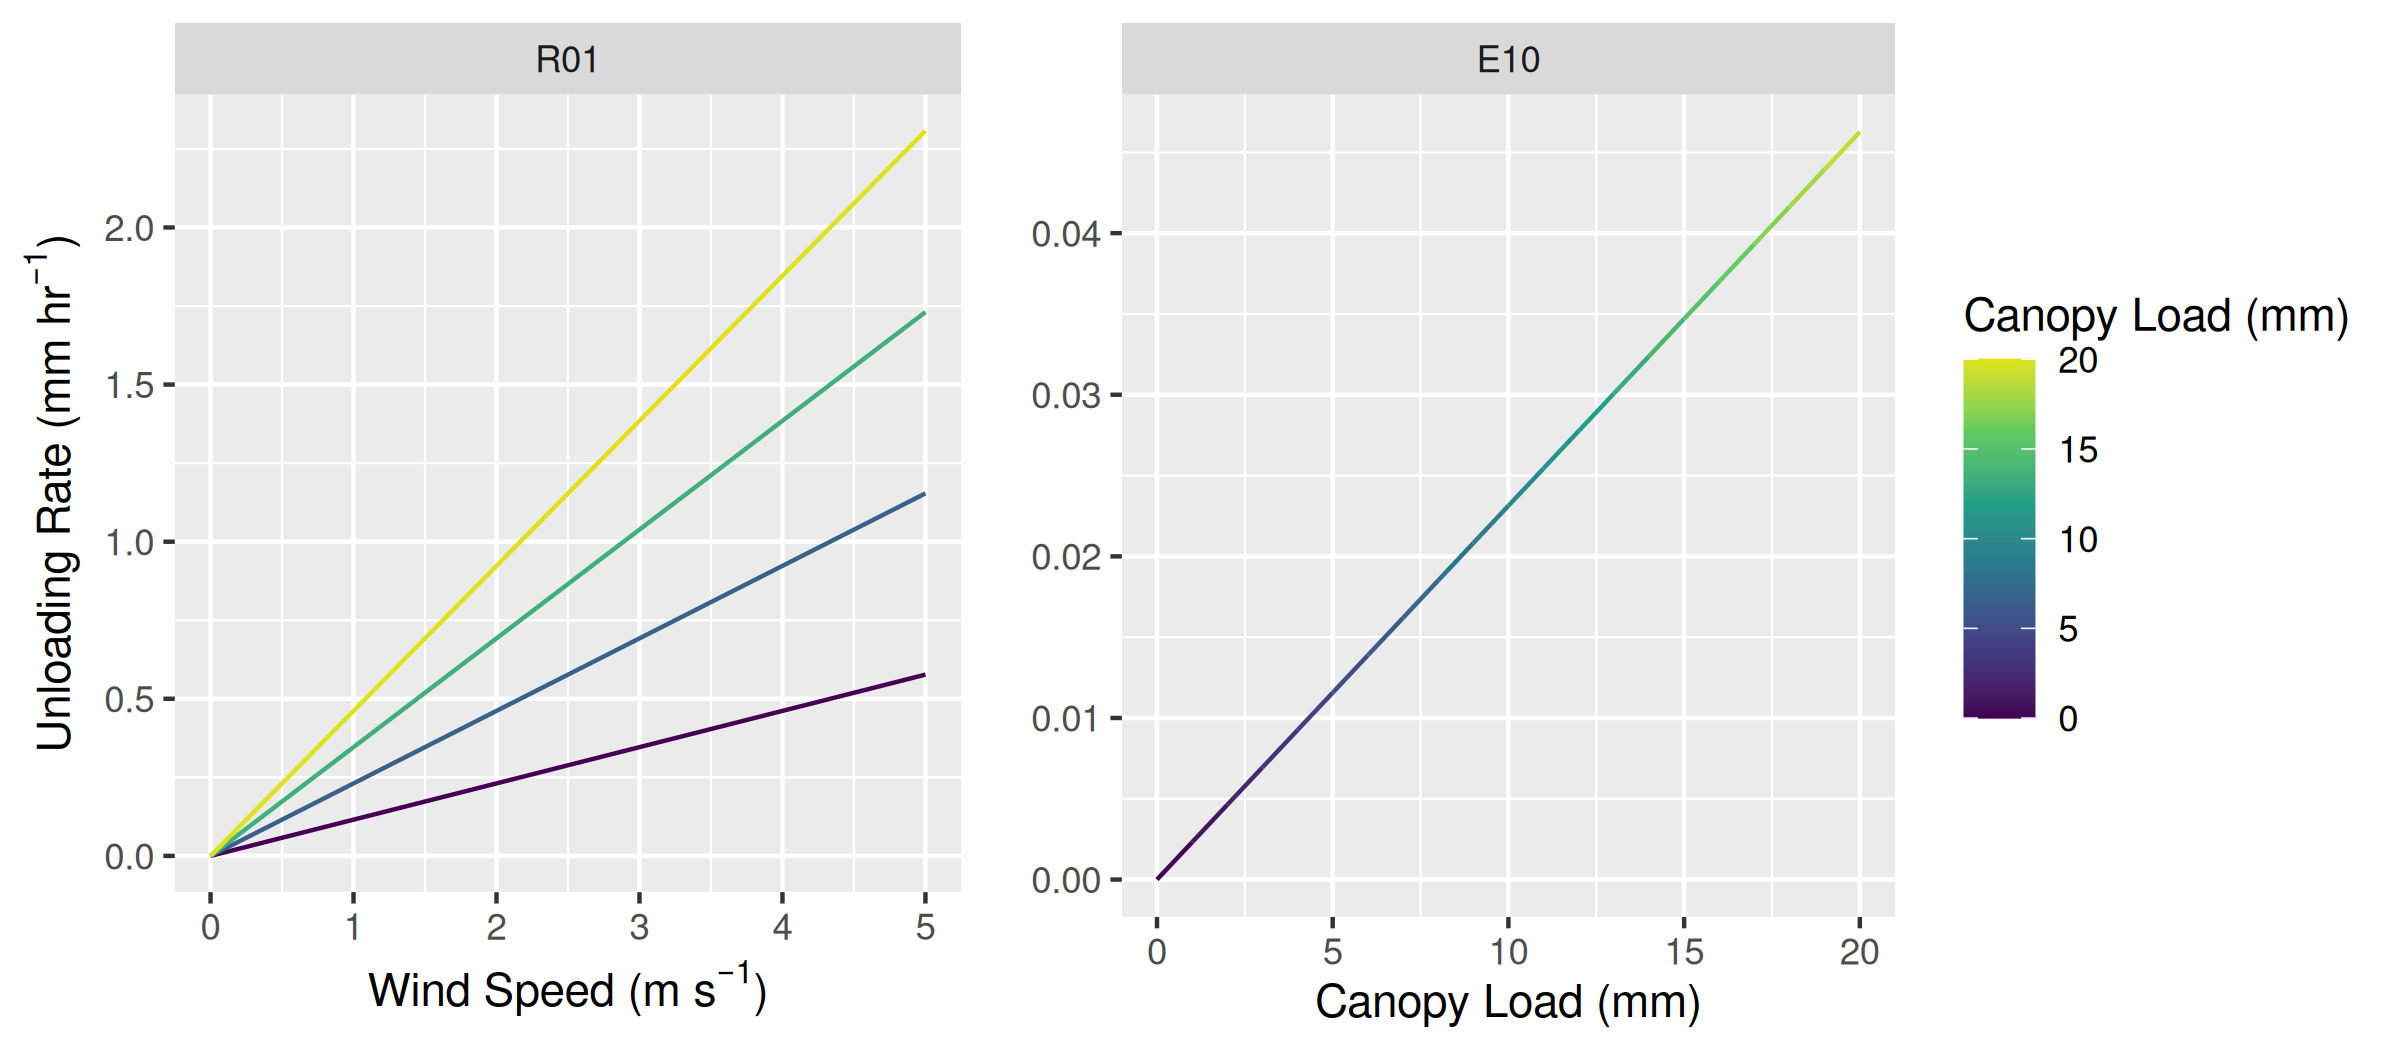
\includegraphics[keepaspectratio]{chapters/04-ablation-paper/figs/figure1.png}}

}

\caption{\label{fig-unl-ex-wind}The Roesch et al. (2001) model of
unloading rate with increasing wind speed and canopy snow load (left,
R01) and the Hedstrom \& Pomeroy (1998) model of unloading rate with
increasing snow load (right, E10). Both examples have a constant air
temperature of -10°C to disable the influence of warming on unloading
and drip.}

\end{figure}%

\begin{figure}

\centering{

\pandocbounded{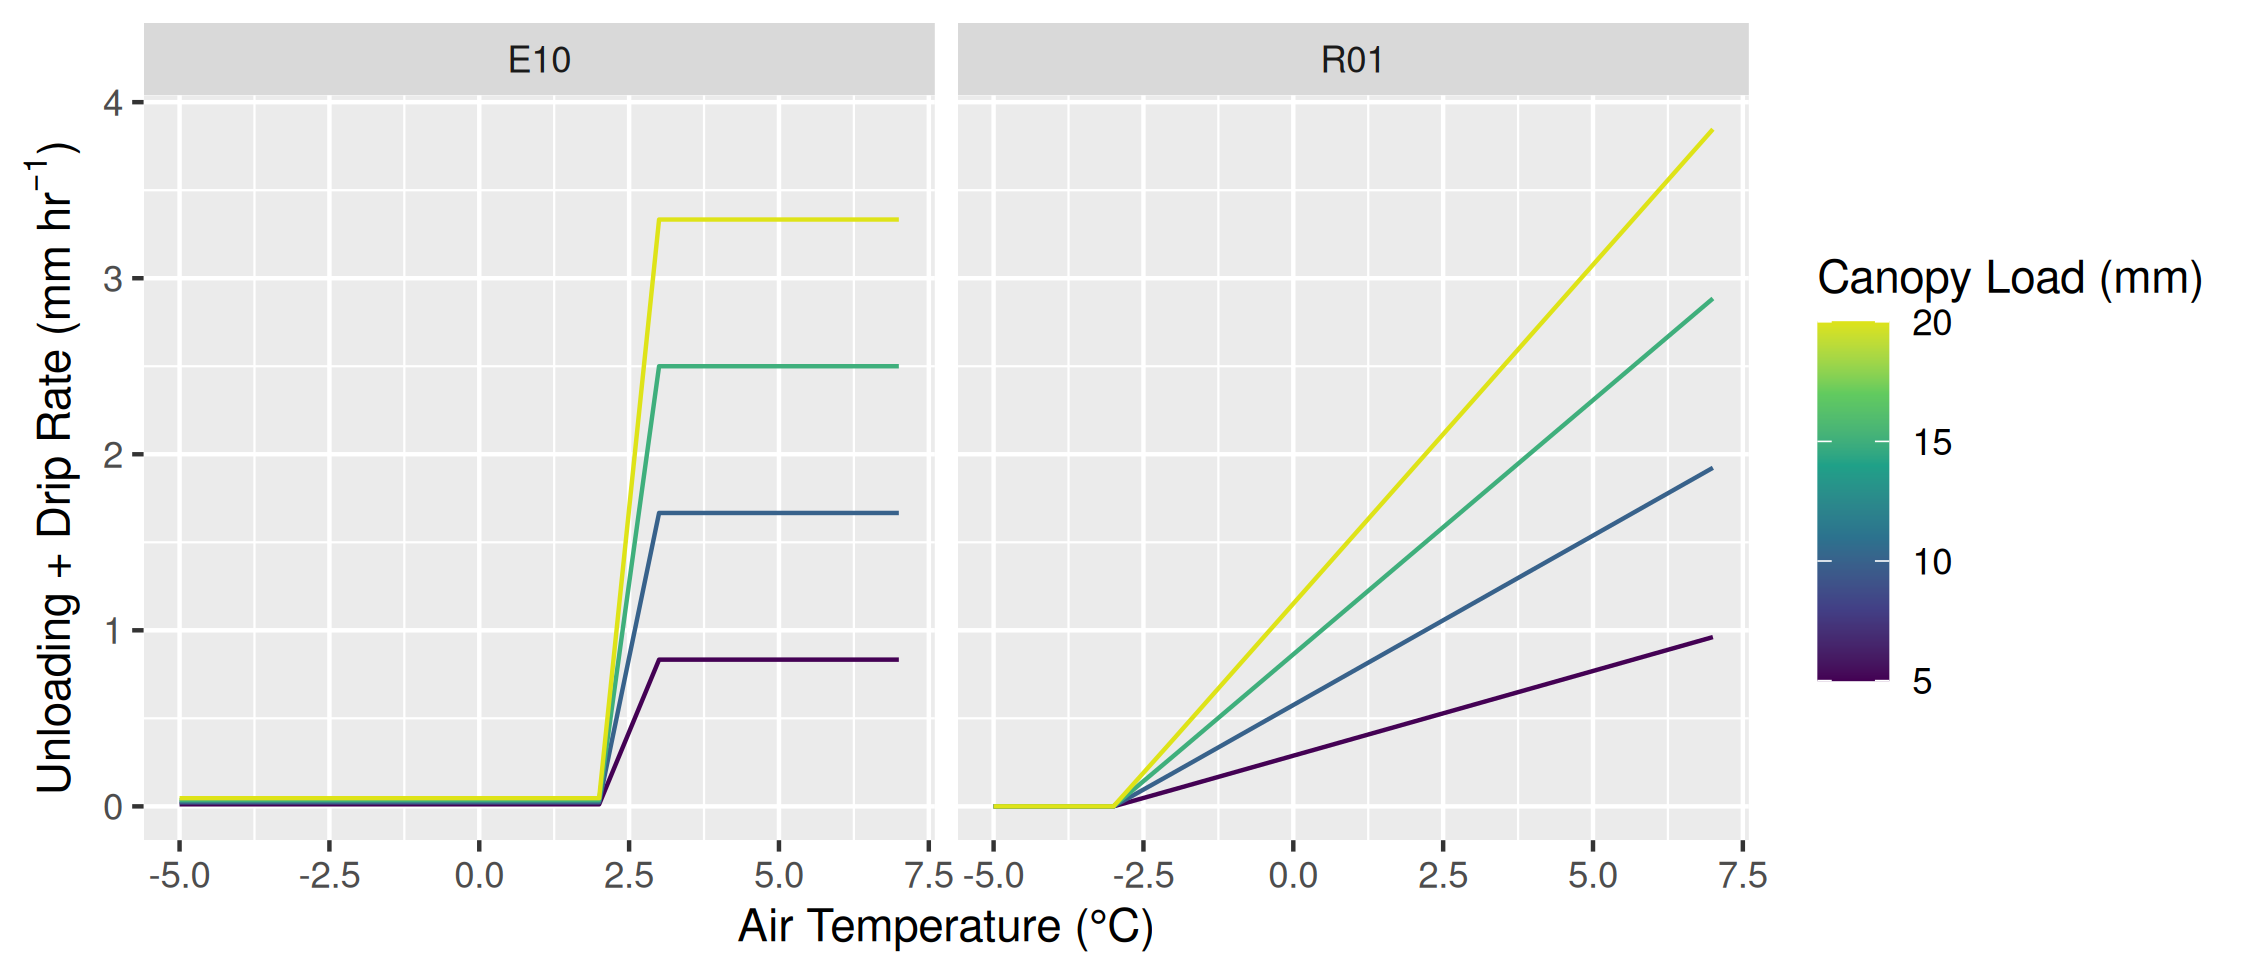
\includegraphics[keepaspectratio]{chapters/04-ablation-paper/figs/figure2.png}}

}

\caption{\label{fig-unl-ex-temp}The Ellis et al. (2010) and Floyd (2012)
(E10) model of unloading and drip rate (left) and the Roesch et al.
(2001) (R01) model of unloading rate (right) with increasing air
temperature. Wind speed for the R01 parameterisation was set to zero.}

\end{figure}%

\section{Methods}\label{methods}

\subsection{Study Site}\label{study-site-1}

The observations presented in this study were collected at Fortress
Mountain Research Basin (FMRB), Alberta, Canada, -115° W, 51° N, a
continental headwater basin in the Canadian Rockies. The site is located
2100 m above sea level on a ridge covered by mature fir and spruce
forest. Air temperature, humidity, and wind speed were measured at a
height of 4.3 m at Forest Tower (FT) Station
(Figure~\ref{fig-site-map}). Shear stress was calculated using the
EddyPro software (LI-COR Biosciences) based on high-frequency wind
measurements from a CSAT3 three-dimensional sonic anemometer (Campbell
Scientific) installed at 3.0 m at FT station. The CSAT3 was occasionally
covered in snow during the analysis period, and thus to provide a
complete record of shear stress, a linear relationship was established
between shear stress derived from the CSAT3 and the square of wind speed
measured at 4.3 m at the FT station (\emph{R\textsuperscript{2}} = 0.71,
\emph{p} \textless{} 0.05). This relationship was then used to gap-fill
shear stress during periods when the CSAT3 was snow-covered. The
precipitation rate was measured by an Alter-shielded OTT Pluvio weighing
precipitation gauge installed 2.6 m above ground at the adjacent
Powerline (PWL) Station (Figure~\ref{fig-site-map}). Incoming and
outgoing solar radiation was measured by a Kipp \& Zonen CNR4
4-Component Net Radiometer installed 3.27 m above the ground at Fortress
Ridge Station (FRS) 2.0 km to the northwest of FT station (-115.2° W,
50.8° N). This windy exposed site was selected to reduce snow
accumulation on the radiometers, in addition to the CNR4's built-in
heating element. Three subcanopy lysimeters, consisting of plastic
horse-watering troughs with an opening of 0.9 m\textsuperscript{2} and
depth of 20 cm suspended from a load cell, were installed to measure
subcanopy snow accumulation. A weighed tree lysimeter (subalpine fir)
suspended from a load cell (Artech S-Type 20210-100) measured the weight
of canopy snow load (kg) and was scaled to an areal estimate of snow
load (mm) using snow surveys as in Pomeroy \& Schmidt (1993). To isolate
the subcanopy lysimeter measurements of canopy snow unloading from
throughfall, 15-min intervals were selected that had no atmospheric
precipitation based on the precipitation gauge at PWL. The weighed tree
and timelapse imagery also were used to confirm there was no atmospheric
precipitation and to identify periods where snow was intercepted in the
canopy and ablation was possible. Four tipping bucket rain gauges---3
Texas Electronics TR-525M and 1 Hyquest Solutions TB4MM---were installed
along a 15 m transect adjacent to the dense canopy subcanopy lysimeter
to quantify sub-canopy drip from melting intercepted snow. Additional
details on this study site and the meteorological and lysimeter
measurements have been described in Cebulski \& Pomeroy (2025b).

\begin{figure}

\centering{

\pandocbounded{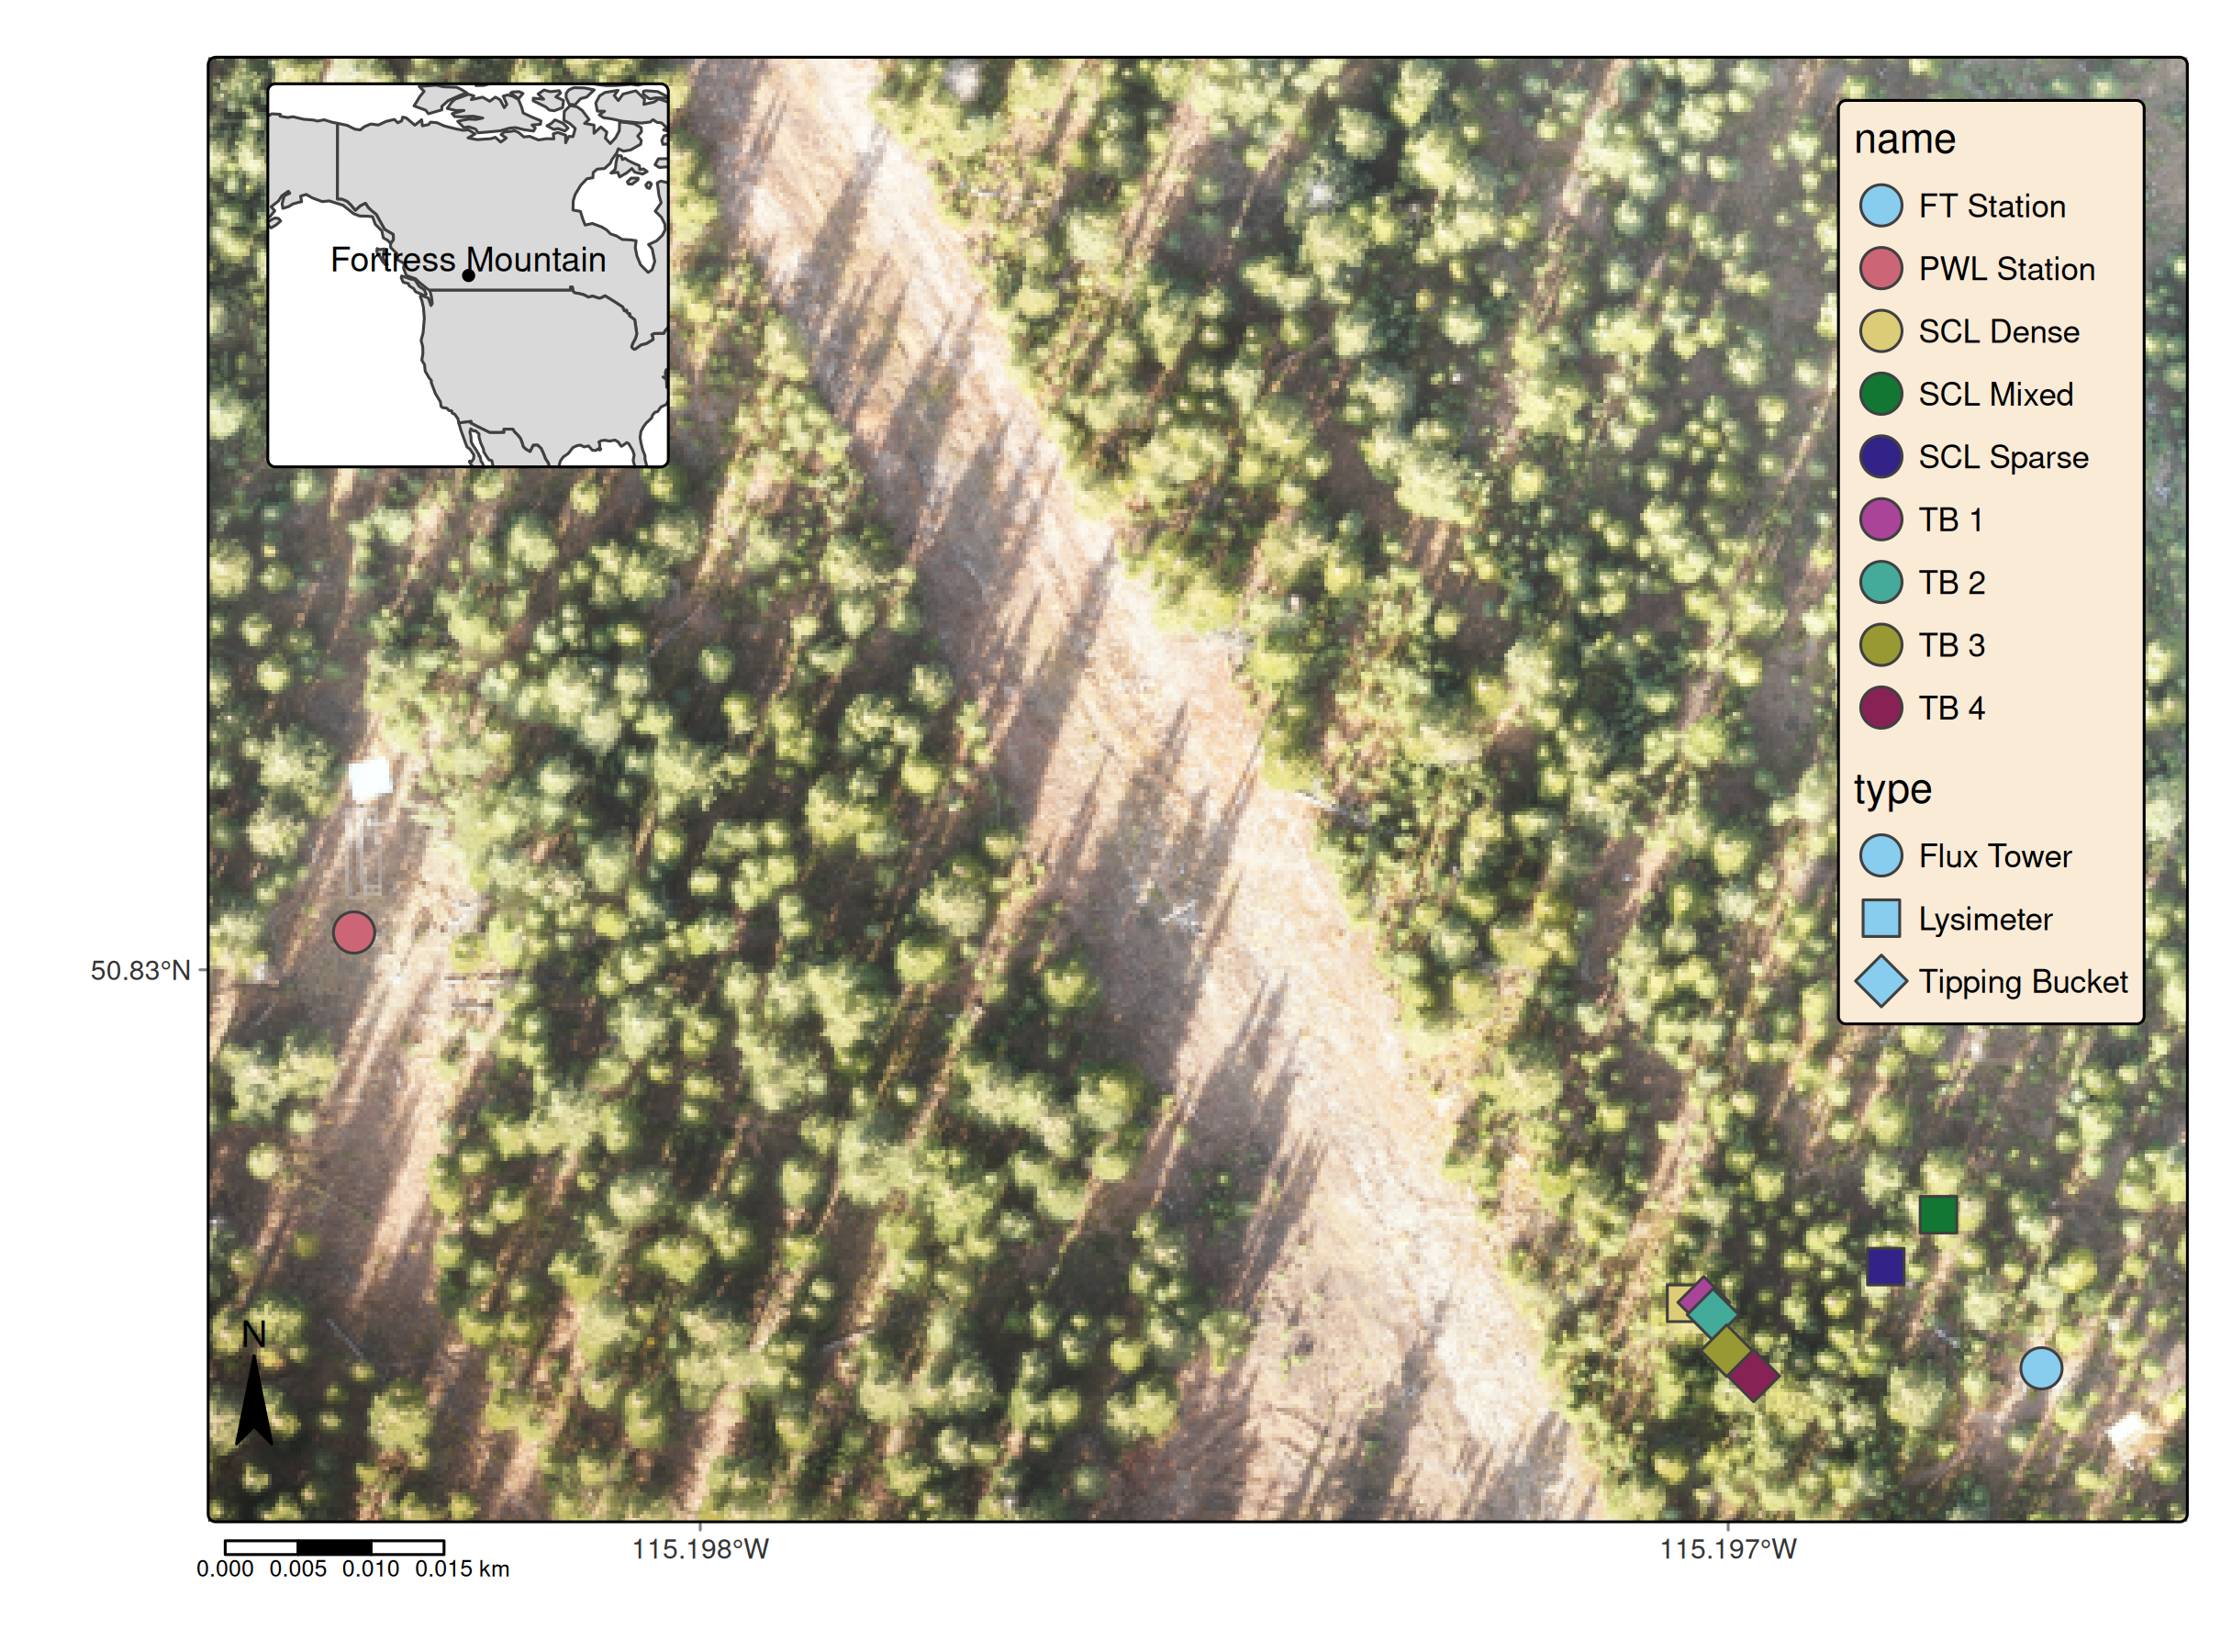
\includegraphics[keepaspectratio]{chapters/04-ablation-paper/figs/figure3.png}}

}

\caption{\label{fig-site-map}Map showing the location of flux towers and
lysimeter instruments. The inset map on the upper left shows the
regional location of Fortress Mountain Research basin. Flux towers are
denoted by a circle, lysimeters by a square, and tipping bucket rain
gauges (TB) by diamonds.}

\end{figure}%

\subsection{The Cold Regions Hydrological Model
Platform}\label{the-cold-regions-hydrological-model-platform}

The Cold Regions Hydrological Model Platform (CRHM) was used to
implement calculations of the canopy snow energy and mass budget. A full
description of the CRHM platform is described in Pomeroy et al. (2022)
and the source code is available at
https://github.com/srlabUsask/crhmcode. The climate forcing data used to
run CRHM was from station-based fifteen-minute interval measurements of
air temperature, relative humidity, wind speed, precipitation, and
incoming solar radiation from the FT, PWL, and FRS stations. CRHM
incorporates a flexible modular design allowing the user to select
various modules (parameterisations) that represent hydrological
processes. The phase of atmospheric precipitation was determined from
the energy balance of falling hydrometeors (Harder \& Pomeroy, 2013). A
new CRHM module was created here to simulate the coupled mass and energy
balance of snow intercepted in the canopy. The energy balance is
described in detail in Section~\ref{sec-ebal} and the updates to the
mass balance through revisions to the canopy snow unloading empirical
functions are presented in Section~\ref{sec-dry-unld} and
Section~\ref{sec-melt-unld}.

\subsection{Canopy Snow Mass Balance}\label{sec-mbal}

The following mass balance as described in Cebulski \& Pomeroy (2025a)
was implemented in CRHM to track the state of canopy snow load (\(L\),
mm) over time:

\begin{equation}\phantomsection\label{eq-canopy-mass-bal}{
\frac{dL}{dt} = 
[q_{sf} - q_{tf} + q_{ros}] - [q_{unld}^{melt} + q_{unld}^{dry}] - q_{drip} - q_{wind}^{veg} - q_{sub}^{veg}
}\end{equation}

where \(\frac{dL}{dt}\) is the change in canopy snow load over time, (mm
s\textsuperscript{-1}), \(q_{sf}\) is the snowfall rate (mm
s\textsuperscript{-1}), \(q_{tf}\) is the throughfall rate (mm
s\textsuperscript{-1}), \(q_{ros}\) is the rate of rainfall falling on
snow intercepted in the canopy (mm s\textsuperscript{-1}),
\(q_{unld}^{melt}\) is the unloading rate due to melt (mm
s\textsuperscript{-1}), \(q_{unld}^{dry}\) is the dry snow unloading
rate due to shear stress on snow, wind erosion, branch movement,
structural degradation, bond weakening and increased elasticity of
branches and other non-melt related processes (mm
s\textsuperscript{-1}), \(q_{drip}\) is the canopy snow drip rate (mm
s\textsuperscript{-1}) resulting from canopy snowmelt (\(q_{melt}\), mm
s\textsuperscript{-1}), \(q_{wind}^{veg}\) is the wind transport rate in
or out of the control volume (mm s\textsuperscript{-1}), and
\(q_{sub}^{veg}\) is the intercepted snow sublimation rate (mm
s\textsuperscript{-1}) which includes any evaporation of liquid water in
the canopy. Figure 1 in Cebulski \& Pomeroy (2025a) presents a visual
representation of this mass balance.

\subsection{Mass Balance
Parameterisations}\label{mass-balance-parameterisations}

In addition to the updated canopy snow model presented in this study,
hereafter referred to as CP25 (described in Section~\ref{sec-dry-unld}
and Section~\ref{sec-melt-unld}), three other canopy snow models were
implemented in CRHM following previous studies by Ellis et al. (2010)
and Floyd (2012) (E10), Roesch et al. (2001) (R01), and Andreadis et al.
(2009) who built on observations by Storck et al. (2002) (SA09). The E10
model includes canopy snow sublimation as described in Pomeroy et al.
(1998b), dry snow unloading as a function of canopy snow load from
Hedstrom \& Pomeroy (1998) with modifications described in Ellis et al.
(2010) and Floyd (2012) to handle canopy snow melt and drip processes
using an ice-bulb temperature threshold. The R01 model represents dry
snow unloading, melt, and drip using linear functions of wind speed and
air temperature, while sublimation is simulated using the
parameterisation from Pomeroy et al. (1998b). The SA09 model unloads
snow as a ratio of the canopy snowmelt rate, following observations by
Storck et al. (2002) and does not include dry snow unloading. The
snowmelt rate from Equation~\ref{eq-eb} was used to calculate the
unloading rate for the Andreadis et al. (2009) unloading and thus
differs from the energy balance routine described in their study. Canopy
snow sublimation in SA09 was represented based on the Essery et al.
(2003) parameterisation (Equation~\ref{eq-ql}) as implemented in CP25.

The retention of canopy snow meltwater differs between the four canopy
snow models implemented in CRHM. For E10, liquid meltwater is not
retained in the canopy and immediately drips before it can evaporate.
The R01 model also does not represent evaporation of liquid meltwater as
canopy snow is not explicitly separated between solid snow unloading and
melt/drip. The canopy liquid water storage capacity (\(L_{max}^{liq}\),
mm) from SA09 and CP25 was calculated as:

\begin{equation}\phantomsection\label{eq-liq-hold-cap}{
L_{max}^{liq} = Lh + nLAI
}\end{equation}

where \(h\) is the liquid meltwater holding capacity that canopy can
retain against gravity and \(n\) is a storage constant of the vegetation
elements. Andreadis et al. (2009) estimated \(h\) as 0.035 (-) and \(n\)
as \(e^{-4}\). In this study, \(h\) was set to 0.01 (-), and \(n\) was
defined as \(C_c\cdot 0.2\). A one-sided effective plant (leaf) area
index (LAI) was used, including the clumping factor to account for
needleleaf canopy structures, following the approach of Ellis et al.
(2010) for rainfall interception.

\subsection{Canopy Snow Energy Balance}\label{sec-ebal}

The CP25 and SA09 canopy snow models implemented the following energy
balance approach to calculate the energy available for melting snow
intercepted in the canopy (\(Q_{melt}\), W m\textsuperscript{-2}) and to
track the canopy snow temperature over time
(\(\frac{\Delta T_{vs}}{\Delta t}\), K s\textsuperscript{-1}). The
energy balance is expressed as:

\begin{equation}\phantomsection\label{eq-eb}{
Q_{melt} = 
Q_{sw} +
Q_{lw} +
Q_{p} + Q_{h} + Q_{l} - [C_p^{ice} L \frac{\Delta T_{vs}}{\Delta t}]
}\end{equation}

where \(Q_{sw}\) and \(Q_{lw}\) (W m\textsuperscript{-2}) are the net
shortwave and longwave radiation heat fluxes to the canopy snow, \(Q_p\)
(W m\textsuperscript{-2}), is the advective energy rate, and \(Q_{l}\)
and \(Q_{h}\) (W m\textsuperscript{-2}), are the turbulent fluxes of
latent heat and sensible heat respectively (positive towards canopy
snow), and \(C_p^{ice}\) (J kg\textsuperscript{-1}
K\textsuperscript{-1}) is the specific heat capacity of ice. Figure 2 in
Cebulski \& Pomeroy (2025a) shows a visual representation of this energy
balance.

\subsection{Energy Balance
Parameterisations}\label{energy-balance-parameterisations}

The E10 and R01 parameterisations relied on physically guided empirical
relationships to simulate sublimation and melt and are described in full
detail in their respective articles and are also summarised in Cebulski
\& Pomeroy (2025a). The following section describes the energy balance
parameterisations implemented in the CP25 and SA09 models.

\(Q_{sw}\) was determined as:

\begin{equation}\phantomsection\label{eq-sw}{
Q_{sw} = Q_{sw}^{in} \cdot (1 - \alpha_s) \cdot \tau_{50}^{veg}
}\end{equation}

where \(Q_{sw}^{in}\) is the downwelling shortwave radiation (W
m\textsuperscript{-2}), \(\alpha_s\) is the albedo of snow intercepted
in the canopy (-), \(\tau_{50}^{veg}\) (-) is the canopy transmittance
to \(Q_{sw}^{in}\). Equation 10 from Pomeroy et al. (2009) was used to
determine \(\tau_{50}^{veg}\), using half of the leaf area index (LAI)
based on studies Weiskittel et al. (2009) and Kesselring et al. (2024)
that approximately 50\% of the total leaf area is concentrated in the
upper half of coniferous canopies. \(Q_{sw}\) provides an approximation
of the net shortwave radiation to all snow intercepted in the canopy and
is a simplification from using a partial differential equation to
determine the radiation incident to individual height layers within the
canopy. Upwelling shortwave radiation reflected off the surface snowpack
is considered negligible contribution to the snow intercepted in the
canopy as it is primarily blocked by vegetation elements underlying the
canopy snow (Pomeroy et al., 2009).

\(Q_{lw}\) was approximated as:

\begin{equation}\phantomsection\label{eq-lw}{
Q_{lw} = \downarrow Q_{lw}^{atm} + \uparrow Q_{lw}^{veg} - Q_{lw}^{vs}
}\end{equation}

where \(Q_{lw}^{atm}\) is the downwelling longwave radiation from the
atmosphere (W m\textsuperscript{-2}), \(Q_{lw}^{veg}\) is the longwave
radiation upwelling from vegetation elements underlying snow intercepted
in the canopy (W m\textsuperscript{-2}), and \(Q_{lw}^{vs}\) (W
m\textsuperscript{-2}) is the outgoing longwave radiation from the top
and bottom of the canopy snow layer calculated as:

\begin{equation}\phantomsection\label{eq-lw-vs}{
Q_{lw}^{vs} = 2 \epsilon_{s} \sigma T_{vs}^4
}\end{equation}

where \(\epsilon_s\) is the emissivity (-) of snow taken as 0.99 and
\(\sigma\) is the Stefan--Boltzmann (5.67e\textsuperscript{-10} W
m\textsuperscript{-1} K\textsuperscript{-4}). \(Q_{lw}^{atm}\) was
approximated in this study as in Sicart et al. (2006) to represent the
influence of atmospheric moisture and clouds on emissivity.
\(Q_{lw}^{veg}\) was calculated with the assumption that canopy elements
are in equilibrium with the air temperature plus any increase in
vegetation temperature from the extinction of \(Q_{sw}^{in}\) in the
canopy (Pomeroy et al., 2009, Eq. 4).

\(Q_p\) was calculated as:

\begin{equation}\phantomsection\label{eq-qp}{
Q_p = [C_p^{liq} m_r(T_r - T_{vs}) + C_p^{ice} m_s(T_s - T_{vs})] / \Delta t
}\end{equation}

where \(C_p^{liq}\) is the specific heat capacity of liquid water (J
kg\textsuperscript{-1} K\textsuperscript{-1}), \(m_r\) is the specific
mass of liquid water in precipitation (mm), \(T_r\) is the rainfall
temperature (K), \(m_s\) is the specific mass of snow in precipitation
(mm), and \(T_s\) is the snowfall temperature (K).

\(Q_h\) was calculated as:

\begin{equation}\phantomsection\label{eq-qh}{
Q_h = \frac{\rho_a}{r_a} C_p^{air} (T_a - T_{vs})
}\end{equation}

where \(\rho_a\) is the air density (kg m\textsuperscript{-3}),
\(C_p^{air}\) is the specific heat capacity of air (J
kg\textsuperscript{-1} K\textsuperscript{-1}), \(T_a\) is the air
temperature, and \(r_a\) is the aerodynamic resistance (s
m\textsuperscript{-1}) which was approximated from Equation 4 in Allan
et al. (1998) as:

\begin{equation}\phantomsection\label{eq-ra}{
r_a = \frac{\text{log}(\frac{z_T - d_0}{z_0})\text{log}(\frac{z_u - d_0}{z_0})}{\kappa^2 u_z}
}\end{equation}

where \(z_T\) is the height of temperature measurement (m), \(d_0\) is
the displacement height (m) which was approximated as
2/3\textsuperscript{rd} the mean canopy height, \(z_0\) is the roughness
length (m) which was approximated as 1/10\textsuperscript{th} of the
mean canopy height, \(z_u\) is the wind speed measurement height (m),
\(\kappa\) is von Kármán's constant, 0.41 (-), and \(u_z\) is the wind
speed measurement at \(z_u\) (m s\textsuperscript{-1}).

\(Q_l\) was calculated as:

\begin{equation}\phantomsection\label{eq-ql}{
Q_l = \frac{\rho_a}{r_i+r_a} (q_a(T_a) - q_{vs}(T_{vs}))
}\end{equation}

where \(r_i\) is a resistance for transport of moisture from intercepted
snow to the canopy air space (Eq. 28 in Essery et al., 2003),
\(q_a(T_a)\) and \(q_{vs}(T_{vs})\) are the specific humidity (-) at the
air temperature and canopy snow temperature, respectively. \(r_i\) was
calculated following the concept of how full the canopy is with snow as
introduced by Pomeroy \& Schmidt (1993) with modifications to
incorporate a larger maximum canopy snow load capacity of 50 mm based on
observations by Storck et al. (2002), Floyd (2012), and Cebulski \&
Pomeroy (2025b).

The above sensible and latent heat flux equations assume neutral
atmospheric stability conditions, which is supported by the uncertainty
of stability correction in forest canopies (Conway et al., 2018) and
mountain environments in winter (Helgason \& Pomeroy, 2012a). Solving
Equation~\ref{eq-eb} requires an iterative solution to determine
\(\Delta T_{vs}\) and the remaining terms which are also a function of
\(T_{vs}\).

\subsection{Influence of Predictive Variables on
Unloading}\label{influence-of-predictive-variables-on-unloading}

The effects of air temperature, wind speed, snow load, melt, and
sublimation on the unloading process were assessed using a multivariate
ordinary least squares regression. The following hypotheses were tested:

\begin{enumerate}
\def\labelenumi{\alph{enumi}.}
\tightlist
\item
  Melt promotes unloading through loss of structural integrity, particle
  bond weakening, and lubrication of intercepted snow.
\item
  Sublimation promotes unloading via structural degradation and bond
  weakening of intercepted snow.
\item
  Wind drag promotes unloading through shear stress applied to
  intercepted snow, wind erosion through direct entrainment in the
  atmosphere of intercepted snow, and branch movement.
\item
  Increasing air temperature promotes unloading by increasing the
  elasticity of branches and its association with melt and/or
  sublimation.
\end{enumerate}

Since these processes occur simultaneously and could not be isolated
experimentally, different combinations of the independent variables were
included in the regression to identify which sets of processes
significantly influenced unloading. The subcanopy lysimeter unloading
measurements had a high relative instrument error due to the relatively
small accumulation of unloaded snow over the 15-min intervals. To
improve instrument accuracy, whilst maintaining consistency of the
unloading measurements with the independent variables, the 15-min
interval measurements of unloading were aggregated over differing
predictive variable bins. Independent variable bins that had less than
0.1 mm of accumulated snow were removed, resulting in a mean instrument
error of +/- 2\% for the remaining bins. Air temperature and wind speed
were measured at the FT station, canopy snow load from the weighed tree
lysimeter (scaled to the canopy of each respective subcanopy lysimeter),
and canopy snowmelt and sublimation simulated using CRHM with the CP25
model as described in the previous section. The individual processes
found to be significant predictors of unloading in the multivariate
regression (i.e., shear stress and canopy snow melt) were isolated to
parameterise a model of their effects that was implemented in the CP25
model.

\subsubsection{Dry Snow Unloading}\label{dry-snow-unloading}

Wind, shear stress, and canopy snow load were assessed as predictors of
dry snow unloading during intervals without canopy snowmelt. These
periods were defined using simulated canopy snowmelt in CRHM as well as
visual analysis of time-lapse imagery for canopy snow drip and/or icicle
formation. The relationships between wind speed, shear stress, canopy
snow load, and unloading were analyzed using linear and non-linear least
squares regressions, linearly with shear stress and exponentially with
wind speed. The linear relationship between shear stress, canopy load,
and unloading did not include an intercept term and was thus the
coefficient of determination (\emph{R\textsuperscript{2}}) was adjusted
following (Kozak \& Kozak, 1995).

\subsubsection{Canopy Snowmelt Induced
Unloading}\label{canopy-snowmelt-induced-unloading}

A mass balance approach was incorporated to determine the unloading rate
resulting from canopy snowmelt (\(q_{unld}^{melt}\), mm
s\textsuperscript{-1}). The effect of the canopy snowmelt rate
(\(q_{melt}\)) on unloading was then assessed by fitting a linear model
using an ordinary least squares regression. Since direct measurements of
canopy snow unloading are challenging to obtain independently from
canopy snowmelt drainage (Storck et al., 2002), the mass balance
introduced in Equation~\ref{eq-canopy-mass-bal} was incorporated to
determine \(q_{unld}^{melt}\) as a residual. During intervals without
\([q_{sf} - q_{tf} + q_{ros}]\) or \(q_{wind}^{veg}\)
Equation~\ref{eq-canopy-mass-bal} was simplified and rearranged to:

\begin{equation}\phantomsection\label{eq-unld-melt-mass-bal}{
q_{unld}^{melt} = -\frac{dL}{dt} - q_{drip} - q_{unld}^{dry} - q_{sub}^{veg}
}\end{equation}

While some components of the canopy snow mass balance can be measured
directly, such as \(\frac{\Delta L}{\Delta t}\) with the weighed tree,
sublimation of canopy snow is more difficult to quantify directly
especially in forested mountain environments (Conway et al., 2018;
Harding \& Pomeroy, 1996; Helgason \& Pomeroy, 2012b; Parviainen \&
Pomeroy, 2000) and thus \(q_{sub}^{veg}\) was simulated in this study in
CRHM using Equation~\ref{eq-ql} as described in Essery et al. (2003).
\(q_{drip}\) was measured where possible using the rain gauges, however
problems with freezing of liquid water in the tipping bucket mechanisms
limited the ability to measure \(q_{drip}\) reliably. Thus, \(q_{drip}\)
was also estimated using simulations of canopy snowmelt (\(q_{melt}\))
in CRHM as in Equation~\ref{eq-eb}, with storage limited by the canopy
liquid water holding capacity and drainage of excess water. Canopy snow
ablation periods that were dominated by melt were selected for
calculating \(q_{unld}^{melt}\) where the contribution of
\(q_{unld}^{dry}\) and \(q_{sub}^{veg}\) to canopy snow ablation was
less than 5\%.

\section{Results}\label{results-1}

\subsection{Unloading Relationships}\label{sec-unld-rel}

Amongst the models evaluated, a multivariate linear regression
incorporating canopy snow load, canopy snowmelt, and wind speed provided
the highest explanatory power for predicting canopy snow unloading
measured by subcanopy lysimeters (\emph{R\textsuperscript{2}} = 0.79, p
\textless{} 0.05; Table~\ref{tbl-q-unld-bins}). Shear stress was found
to explain less variability compared to wind speed, when both were
combined with canopy snow load and snowmelt (\emph{R\textsuperscript{2}}
= 0.71, \emph{p} \textless{} 0.05). Air temperature and canopy snow
sublimation were not significant predictors in any model (\emph{p}
\textgreater{} 0.05; Table~\ref{tbl-q-unld-bins}). A model including
only canopy load, air temperature, and wind speed produced an
\emph{R\textsuperscript{2}} of 0.11 however, only canopy load and wind
speed were statistically significant (\emph{p} \textless{} 0.05). As
shown in Figure~\ref{fig-q-unld-all-bins}, unloading rates varied more
with snowmelt and sublimation (0--2 mm hr\textsuperscript{-1}) than with
air temperature and wind speed (0--0.5 mm hr\textsuperscript{-1}).

The mean unloading rate was observed to increase with increasing canopy
load, air temperature, ice-bulb temperature depression, shear stress,
and wind speed (Figure~\ref{fig-q-unld-all-bins}). An increase in
unloading was found with sublimation rates between 0---0.3 mm
hr\textsuperscript{-1} (Figure~\ref{fig-q-unld-all-bins}). For
sublimation rates higher than 0.3 mm hr\textsuperscript{-1}, unloading
declined with sublimation. The decline in unloading with wind speed
\textgreater3 m s\textsuperscript{-1} might have been contributed to by
wind transport and entrainment into the atmosphere, and/or increased
sublimation rates at higher wind speeds.

\begin{longtable}[]{@{}
  >{\raggedright\arraybackslash}p{(\linewidth - 18\tabcolsep) * \real{0.1000}}
  >{\raggedright\arraybackslash}p{(\linewidth - 18\tabcolsep) * \real{0.1100}}
  >{\raggedright\arraybackslash}p{(\linewidth - 18\tabcolsep) * \real{0.1100}}
  >{\raggedright\arraybackslash}p{(\linewidth - 18\tabcolsep) * \real{0.1100}}
  >{\raggedright\arraybackslash}p{(\linewidth - 18\tabcolsep) * \real{0.1100}}
  >{\raggedright\arraybackslash}p{(\linewidth - 18\tabcolsep) * \real{0.1100}}
  >{\raggedright\arraybackslash}p{(\linewidth - 18\tabcolsep) * \real{0.1100}}
  >{\raggedright\arraybackslash}p{(\linewidth - 18\tabcolsep) * \real{0.1100}}
  >{\raggedleft\arraybackslash}p{(\linewidth - 18\tabcolsep) * \real{0.0700}}
  >{\raggedleft\arraybackslash}p{(\linewidth - 18\tabcolsep) * \real{0.0800}}@{}}

\caption{\label{tbl-q-unld-bins}Summary of multivariate linear
regression results evaluating all combinations of predictor variables
for canopy snow unloading including: canopy load (\(L\)), wind speed
(\(u\)), canopy snowmelt rate (\(q_{melt}\)), canopy snow sublimation
rate (\(q_{subl}\)), and air temperature (\(T_a\)). Columns \(L\) to
\(T_a\) show the coefficient estimate for each respective term, and the
significance of each term is shown in brackets. Significance codes: * =
p \textless{} 0.05; ns = not significant (p \textgreater{} 0.05). The
models are ranked by their corresponding AIC value.}

\tabularnewline

\toprule\noalign{}
\begin{minipage}[b]{\linewidth}\raggedright
Model Name
\end{minipage} & \begin{minipage}[b]{\linewidth}\raggedright
Intercept
\end{minipage} & \begin{minipage}[b]{\linewidth}\raggedright
\(L\)
\end{minipage} & \begin{minipage}[b]{\linewidth}\raggedright
\(u\)
\end{minipage} & \begin{minipage}[b]{\linewidth}\raggedright
\(q_{melt}\)
\end{minipage} & \begin{minipage}[b]{\linewidth}\raggedright
\(q_{subl}\)
\end{minipage} & \begin{minipage}[b]{\linewidth}\raggedright
\(\tau\)
\end{minipage} & \begin{minipage}[b]{\linewidth}\raggedright
\(T_a\)
\end{minipage} & \begin{minipage}[b]{\linewidth}\raggedleft
\(R^2\)
\end{minipage} & \begin{minipage}[b]{\linewidth}\raggedleft
AIC
\end{minipage} \\
\midrule\noalign{}
\endhead
\bottomrule\noalign{}
\endlastfoot
M1 & -0.11 (ns) & 0.02 (*) & 0.08 (*) & 0.40 (*) & --- & --- & --- &
0.79 & -12.8 \\
M4 & -0.08 (ns) & 0.04 (*) & --- & 0.39 (*) & --- & 0.75 (*) & --- &
0.71 & 5.5 \\
M7 & 0.13 (ns) & 0.02 (*) & --- & 0.32 (*) & -0.22 (ns) & --- & --- &
0.54 & 10.0 \\
M10 & -0.06 (ns) & 0.02 (*) & 0.08 (*) & 0.38 (*) & --- & --- & 0.00
(ns) & 0.52 & -4.4 \\
M24 & -0.00 (ns) & 0.02 (*) & 0.05 (*) & 0.36 (*) & 0.13 (ns) & --- &
--- & 0.37 & -2.0 \\
M40 & 0.07 (ns) & 0.01 (*) & 0.06 (*) & --- & --- & --- & 0.01 (ns) &
0.11 & 2.4 \\
M63 & 0.22 (*) & 0.00 (ns) & -0.01 (ns) & --- & 0.07 (ns) & --- & --- &
-0.02 & 39.8 \\

\end{longtable}

\begin{figure}

\centering{

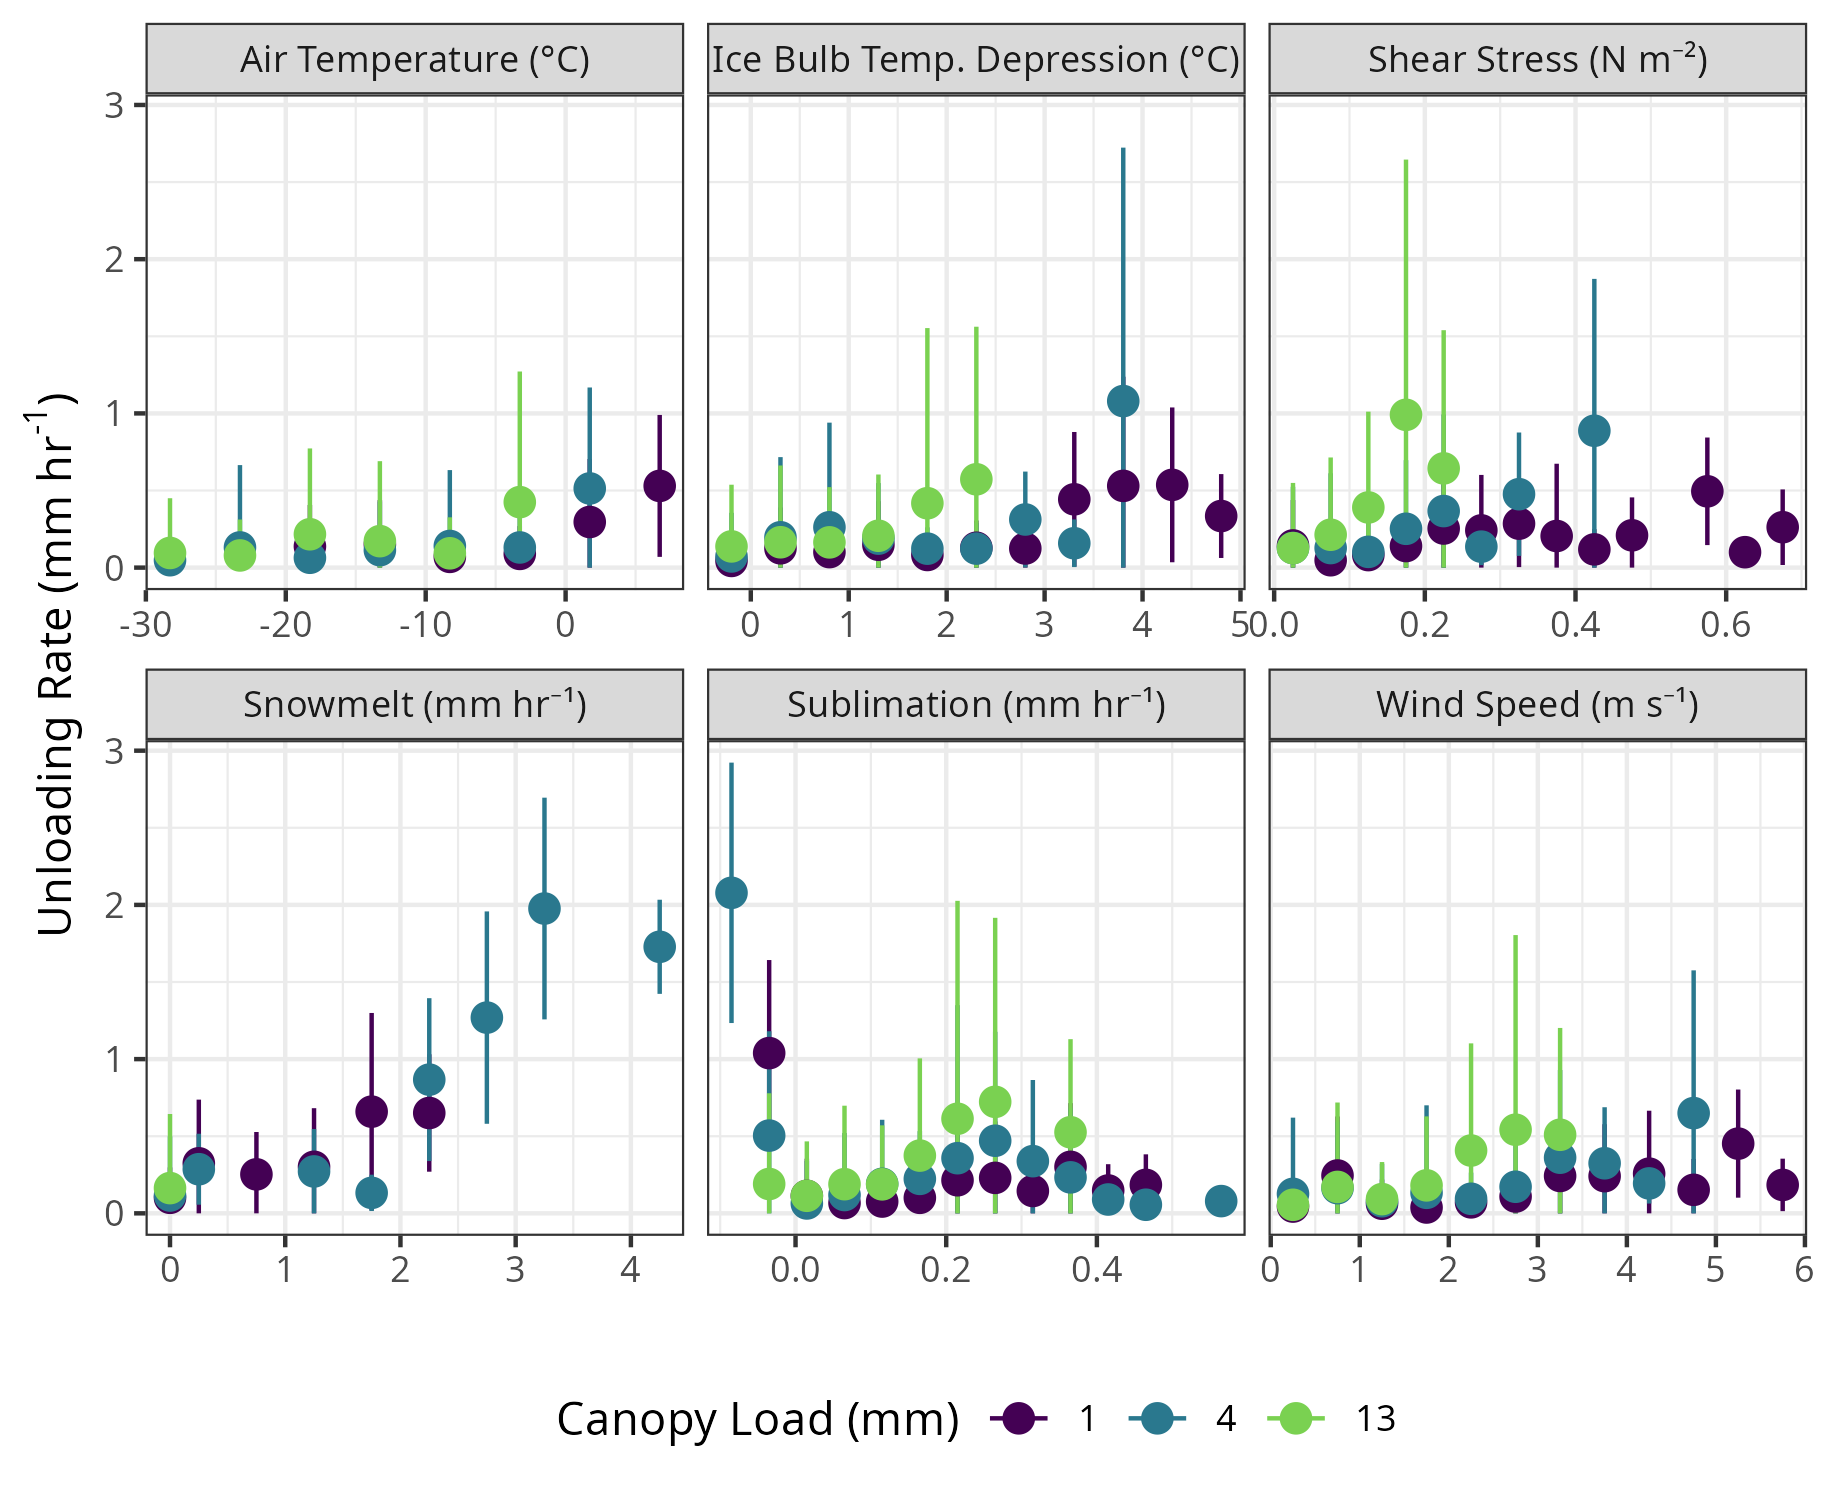
\includegraphics[width=1\linewidth,height=\textheight,keepaspectratio]{chapters/04-ablation-paper/figs/figure4.png}

}

\caption{\label{fig-q-unld-all-bins}Scatter plots showing the mean
unloading rate (mm hr\textsuperscript{-1}) for differing bins of air
temperature (°C), ice-bulb temperature depression (°C), shear stress (N
m\textsuperscript{-2}), canopy snowmelt (mm hr\textsuperscript{-1}),
canopy snow sublimation (mm hr\textsuperscript{-1}), and wind speed (m
s\textsuperscript{-1}). Note: unloading was measured by the subcanopy
lysimeters, air temperature and wind speed were measured at FT station,
canopy snowmelt and sublimation were calculated using CRHM.}

\end{figure}%

\subsubsection{The Influence of Wind on Dry Snow
Unloading}\label{sec-dry-unld}

Canopy snow unloading measured from the subcanopy lysimeters---filtered
to include intervals without canopy snowmelt---were positively
associated in a linear relationship with shear stress and an exponential
relationship with wind speed (Figure~\ref{fig-q-unld-wind}). The
following equations were fitted to these relationships and tested.

The dry unloading rate, \(q_{unld}^{dry}\), was represented as a linear
function of shear stress:

\begin{equation}\phantomsection\label{eq-q-unld-tau}{
q_{unld}^{dry} = L \cdot \tau_{mid} \cdot a
}\end{equation}

where \(\tau_{mid}\) is the shear stress at mid canopy height and \(a\)
is a fitting constant.

An exponential function of wind speed was defined as:

\begin{equation}\phantomsection\label{eq-q-unld-wind}{
q_{unld}^{dry} = L \cdot u_{mid} \cdot a \cdot e^{b\cdot u_{mid}}
}\end{equation}

where \(u_{mid}\) is the wind speed at mid canopy height, and \(a\) and
\(b\) are fitting constants.

The shear stress relationship (Equation~\ref{eq-q-unld-tau}) accounted
for slightly more variability in unloading (\emph{p} \textless{} 0.05,
\emph{R\textsuperscript{2}} = 0.61) compared to wind speed (\emph{p}
\textless{} 0.05, \emph{R\textsuperscript{2}} = 0.54)
(Table~\ref{tbl-q-unld-wind}). The mean bias of the shear stress model
of 0.037 mm hr\textsuperscript{-1} was also lower compared to the wind
speed model of 0.048 mm hr\textsuperscript{-1}, additional model error
statistics and fitting coefficients are provided in
Table~\ref{tbl-q-unld-wind}. Both models exhibited considerable scatter,
with notable uncertainty resulting from instrument error and processes
other than wind contributing to unloading
(Figure~\ref{fig-q-unld-wind}). The wind-induced unloading rate was
observed to be higher for greater canopy snow loads
(Figure~\ref{fig-q-unld-wind}). The \emph{R\textsuperscript{2}} of both
the shear stress and wind speed relationships was much higher than the
variance explained by wind speed when including intervals with melting
snow (Table~\ref{tbl-q-unld-bins}). The higher
\emph{R\textsuperscript{2}} of the shear stress model compared to wind
speed, coupled with the better physical representation of kinetic
energy, suggests that shear stress be selected as the independent
variable to predict dry snow unloading in the model evaluation.

\begin{figure}

\centering{

\pandocbounded{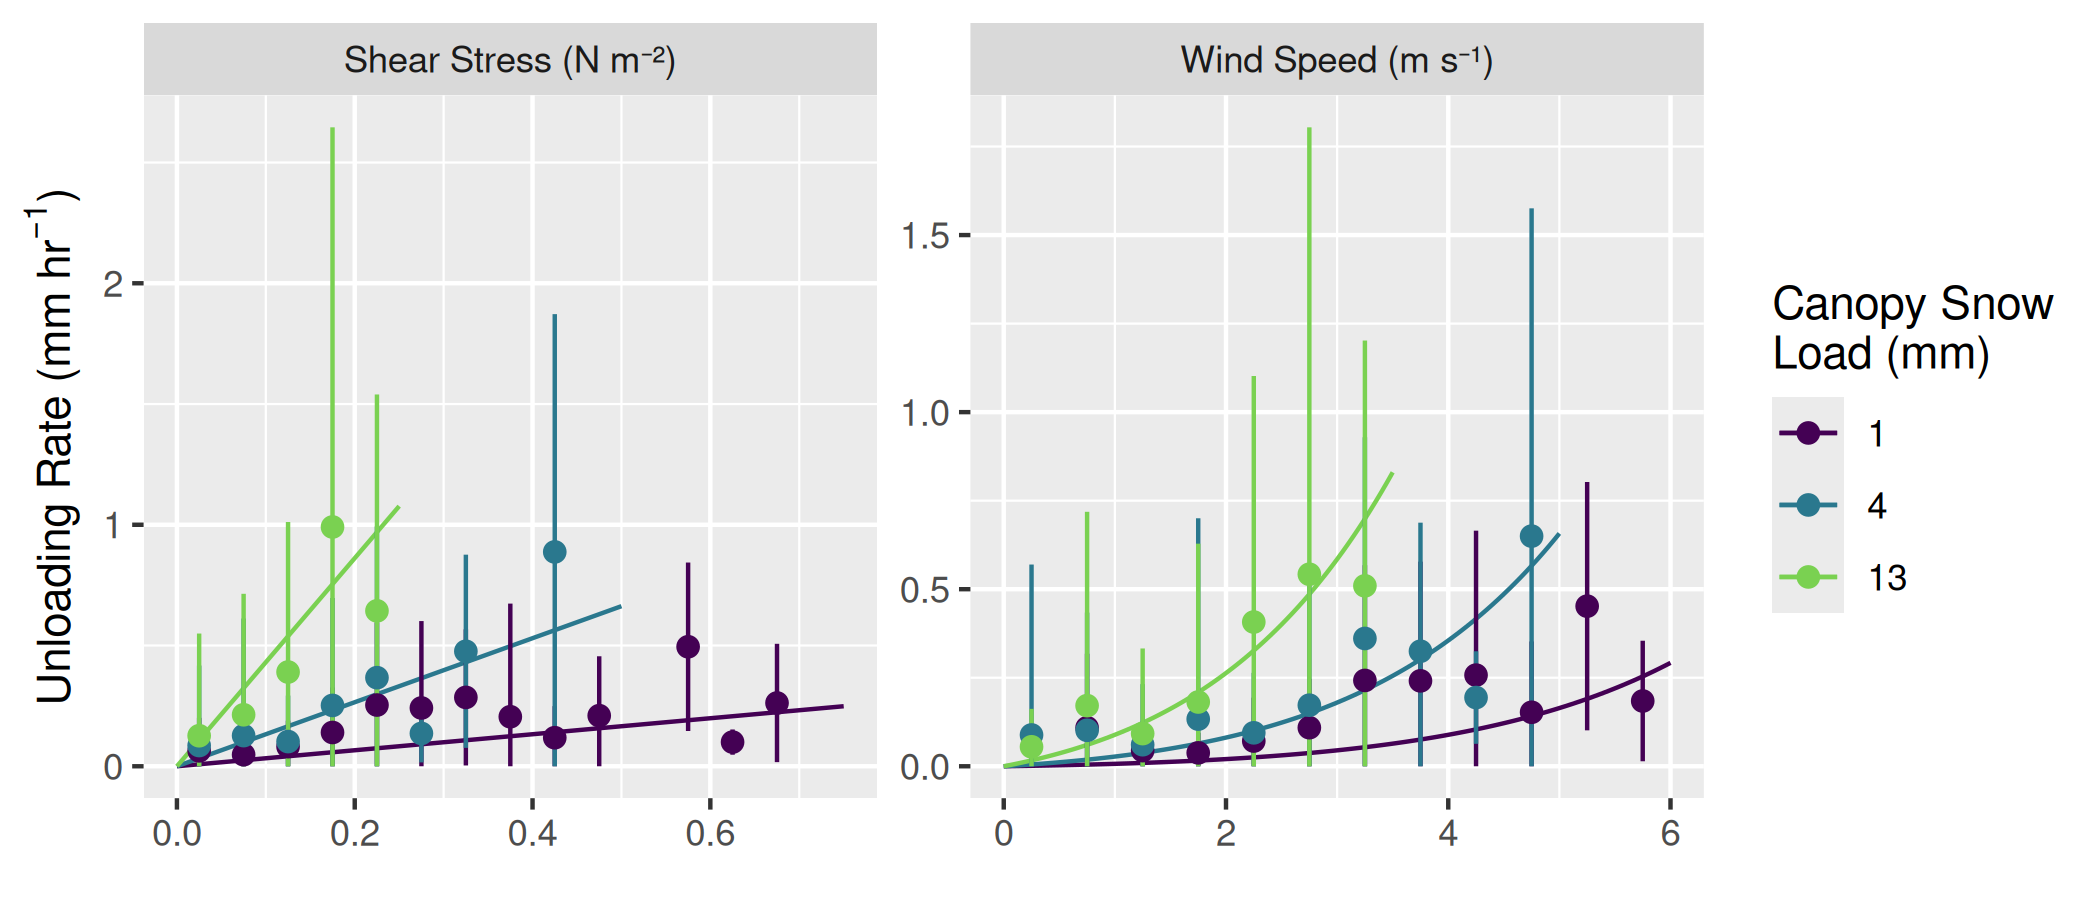
\includegraphics[keepaspectratio]{chapters/04-ablation-paper/figs/figure5.png}}

}

\caption{\label{fig-q-unld-wind}Canopy snow unloading rate measured by
the subcanopy lysimeters versus shear stress (left) and wind speed
(right) during periods without canopy snowmelt. The dots represent mean
unloading rates within bins of shear stress and wind speed for three
canopy snow load levels; error bars indicate +/- 1 standard deviation.
The fitted lines show predictions from Equation~\ref{eq-q-unld-tau}
(left) and Equation~\ref{eq-q-unld-wind} (right).}

\end{figure}%

\begin{longtable}[]{@{}
  >{\raggedright\arraybackslash}p{(\linewidth - 4\tabcolsep) * \real{0.4458}}
  >{\raggedright\arraybackslash}p{(\linewidth - 4\tabcolsep) * \real{0.2771}}
  >{\raggedright\arraybackslash}p{(\linewidth - 4\tabcolsep) * \real{0.2771}}@{}}

\caption{\label{tbl-q-unld-wind}Summary of regression error statistics
and coefficients for the relationship between canopy snow unloading with
wind speed (Equation~\ref{eq-q-unld-tau}) and shear stress
(Equation~\ref{eq-q-unld-wind}), as shown in
Figure~\ref{fig-q-unld-wind}. Coefficients are shown for hourly
unloading.}

\tabularnewline

\toprule\noalign{}
\begin{minipage}[b]{\linewidth}\raggedright
Metric
\end{minipage} & \begin{minipage}[b]{\linewidth}\raggedright
Wind
\end{minipage} & \begin{minipage}[b]{\linewidth}\raggedright
Shear Stress
\end{minipage} \\
\midrule\noalign{}
\endhead
\bottomrule\noalign{}
\endlastfoot
Mean Bias (mm/hr) & 0.048 & 0.037 \\
Mean Absolute Error (mm/hr) & 0.087 & 0.115 \\
Root Mean Square Error (mm/hr) & 0.11 & 0.15 \\
Coefficient of Determination (\(R^2\)) & 0.54 & 0.61 \\
Coefficient a & \(4.62 \times 10^{-03}\) & \(3.31 \times 10^{-01}\) \\
Significance of a & p \textless{} 0.05 & p \textless{} 0.05 \\
Coefficient b & \(3.93 \times 10^{-01}\) & NA \\
Significance of b & p \textless{} 0.05 & NA \\

\end{longtable}

\subsubsection{The Influence of Melt on Unloading}\label{sec-melt-unld}

Five warm \& humid events were selected, in which the median air
temperature was above 0°C and relative humidity was above 65\%,
resulting in less than 5\% contribution of dry snow unloading and
sublimation to ablation as determined by the CP25 model. For these
events, unloading was calculated using
Equation~\ref{eq-unld-melt-mass-bal} and canopy snowmelt rates were
calculated using CRHM with Equation~\ref{eq-eb}. These unloading
estimates were found to be positively correlated with canopy snowmelt
(Figure~\ref{fig-unld-melt-ratio}).

When canopy snow loads remained between 0 and 5 mm, the
unloading-to-melt ratio varied from approximately 0 to 0.5. As snow
loads increased, this ratio increased linearly, reaching its peak value
of 5.0 for a canopy snow load of 30 mm
(Figure~\ref{fig-unld-melt-ratio}). This relationship can be expressed
through a linear function:

\begin{equation}\phantomsection\label{eq-q-unld-melt}{
q_{unld}^{melt} = R \cdot q_{melt}(L)
}\end{equation}

where \(R\) represents the unloading-to-snowmelt ratio and \(q_{melt}\)
is the canopy snowmelt rate (mm hr\textsuperscript{-1}).
Equation~\ref{eq-q-unld-melt} is similar to Equation 33 in Andreadis et
al. (2009); however, instead of a constant value of 0.4 for \(R\), it
was determined as:

\begin{equation}\phantomsection\label{eq-fm}{
R = m \cdot L + b
}\end{equation}

where \(m\) and \(b\) were determined as 0.16 and -0.5, respectively,
using an ordinary least squares regression.
Equation~\ref{eq-q-unld-melt} using these fitted parameters resulted in
a statistically significant relationship (\emph{p} \textless{} 0.05,
\emph{R\textsuperscript{2}} = 0.73) (Figure~\ref{fig-unld-melt-ratio}).
Additional observations of canopy snowmelt from the subcanopy rain
gauges were also used to estimate \(R\)
(Figure~\ref{fig-unld-melt-ratio}). The number of usable observations
was limited to three events (out of the 5 warm \& humid events) due to
freeze-thaw events that seized up the tipping bucket mechanisms in the
rain gauges, however, these measurements are still useful in providing
some validation of the CRHM canopy snowmelt/drip calculations
(Figure~\ref{fig-cml-tb}). The CRHM-estimated cumulative drip was higher
than the subcanopy rain gauges for two out of the three melt events.
Differences in the timing and magnitude of the observed and simulated
values were expected due to both instrument uncertainties in the rain
gauges from freezing of rain gauges and thawing of snow in the
collection funnels, and in the canopy snow energy balance simulation.

\begin{figure}

\centering{

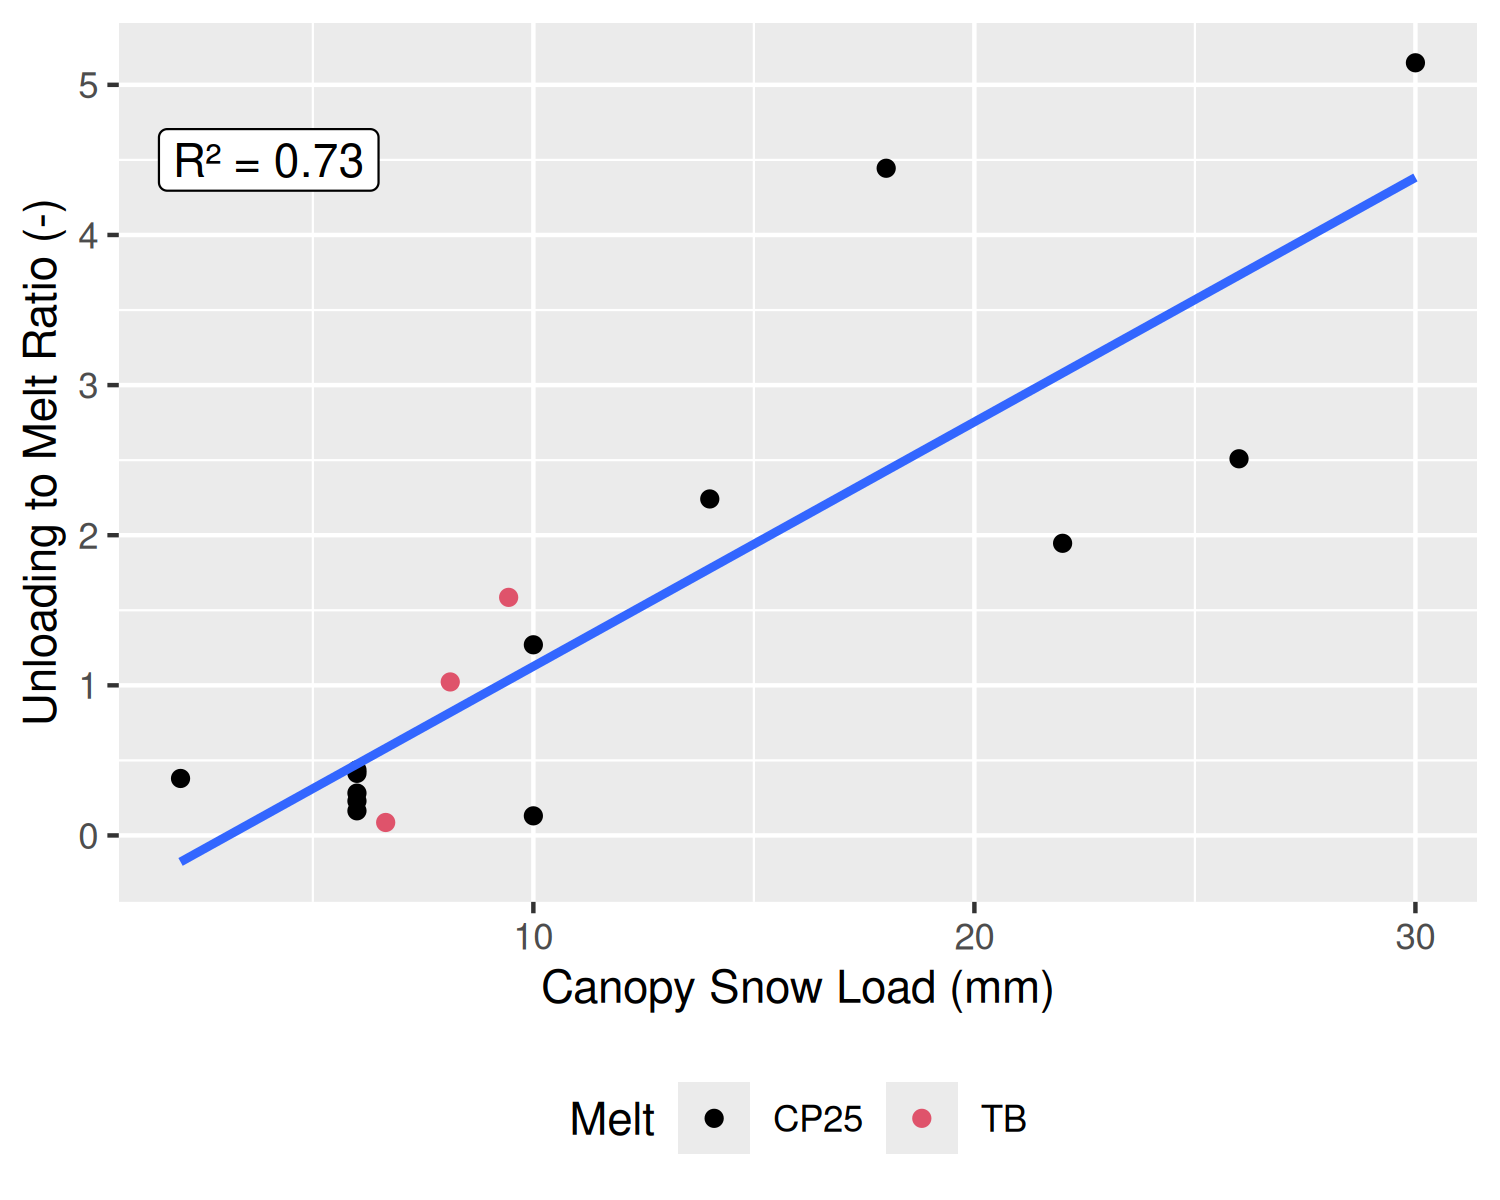
\includegraphics[width=0.8\linewidth,height=\textheight,keepaspectratio]{chapters/04-ablation-paper/figs/figure6.png}

}

\caption{\label{fig-unld-melt-ratio}The ratio of canopy snow unloading
(weighed tree residual) to snowmelt across different canopy snow load
bins and events. Black dots represent the observed cumulative unloading
divided by the cumulative simulated snowmelt from the updated CP25
canopy snow routine in CRHM for each of the five warm \& humid events.
Red dots show the cumulative observed unloading divided by snowmelt
measured by the rain gauges. Multiple dots within a bin correspond to
different events. The blue line represents the best-fit line derived
from ordinary least squares regression.}

\end{figure}%

\begin{figure}

\centering{

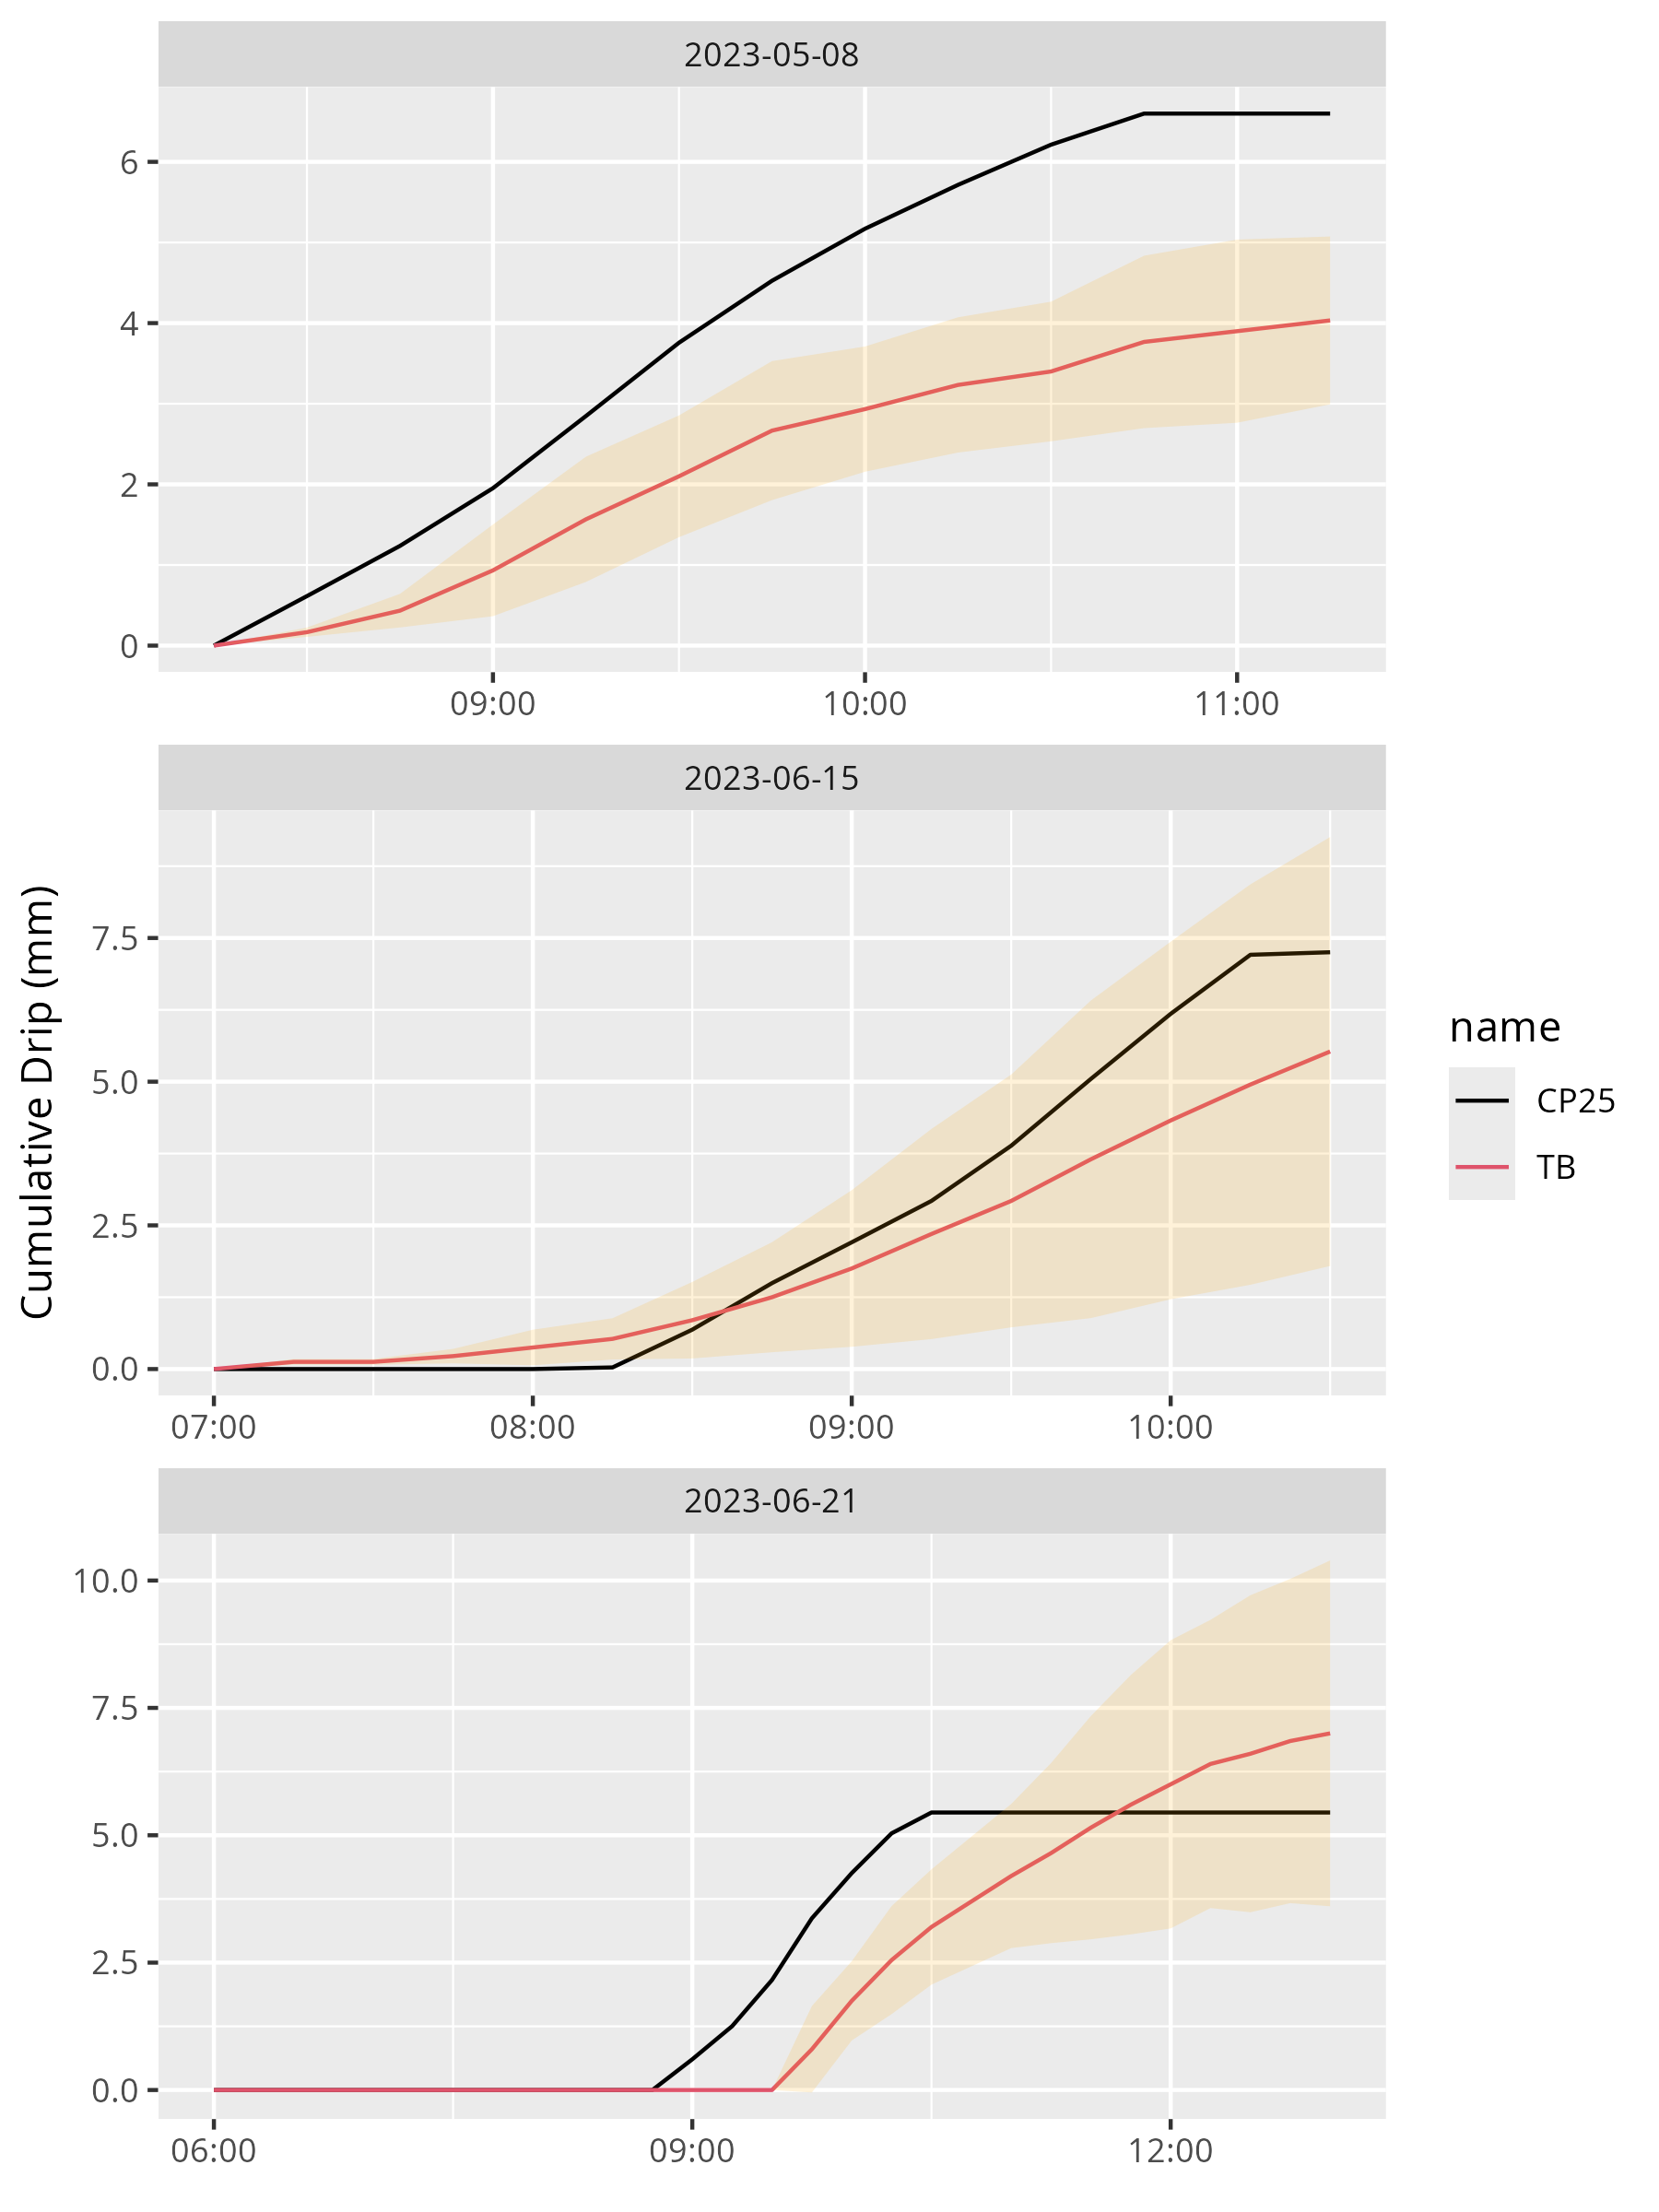
\includegraphics[width=0.85\linewidth,height=\textheight,keepaspectratio]{chapters/04-ablation-paper/figs/figure7.png}

}

\caption{\label{fig-cml-tb}Cumulative canopy snow drip measured by the
average of four subcanopy tipping bucket rain gauges (TB) and simulated
using the CRHM CP25 model (Equation~\ref{eq-eb}). Yellow shading
indicates the range of ±1 standard deviation amongst the individual rain
gauge measurements.}

\end{figure}%

\subsection{New Canopy Snow Model}\label{new-canopy-snow-model}

The CP25 model is based on the canopy snow mass balance formulation
(Equation~\ref{eq-canopy-mass-bal}), where \(q_{tf}\) was represented
as:

\begin{equation}\phantomsection\label{eq-qtf}{
q_{tf} = [(1 - C_p)  \alpha] q_{sf}
}\end{equation}

where \(C_p\) is the leaf contact area calculated using Equation 10 in
Cebulski \& Pomeroy (2025b) and \(\alpha\) is an efficiency constant.
Melt-driven unloading (\(q_{unld}^{melt}\)) was modelled using
Equation~\ref{eq-q-unld-melt}, while dry snow unloading
(\(q_{unld}^{dry}\)) was represented using Equation~\ref{eq-q-unld-tau}.
Canopy snow drip (\(q_{drip}\)) is derived from calculations of canopy
snowmelt from Equation~\ref{eq-eb}, with storage limited by the canopy
liquid water holding capacity computed from
Equation~\ref{eq-liq-hold-cap}; any excess was assumed to immediately
drain. Wind transport of canopy snow (\(q_{wind}^{veg}\)) is
incorporated in the Equation~\ref{eq-q-unld-tau} calculation.
Sublimation of intercepted snow (\(q_{veg}^{sub}\)) was represented
using Equation~\ref{eq-ql}.

\subsection{Event-based Evaluation of Canopy Snow Ablation
Models}\label{event-based-evaluation-of-canopy-snow-ablation-models}

The updated canopy snow model (CP25), as well as the existing models
R01, SA09, and E10 were evaluated using weighed tree lysimeter
measurements of canopy load during seventeen canopy snow ablation
events. The seventeen ablation events had air temperatures ranging from
-30.5°C to +6.9°C and wind speeds from calm to 5.3 m
s\textsuperscript{-1} (Figure~\ref{fig-event-met-boxplot}). This range
of meteorological conditions is particularly wide and spans conditions
typical of the cold boreal to temperate maritime needleleaf forests.
Events were classified as cold \& dry, cold \& humid, warm \& dry, and
warm \& humid based on the median event air temperature (above or below
0°C) and relative humidity (above or below 65\%)
(Figure~\ref{fig-event-met-boxplot}).

\begin{figure}

\centering{

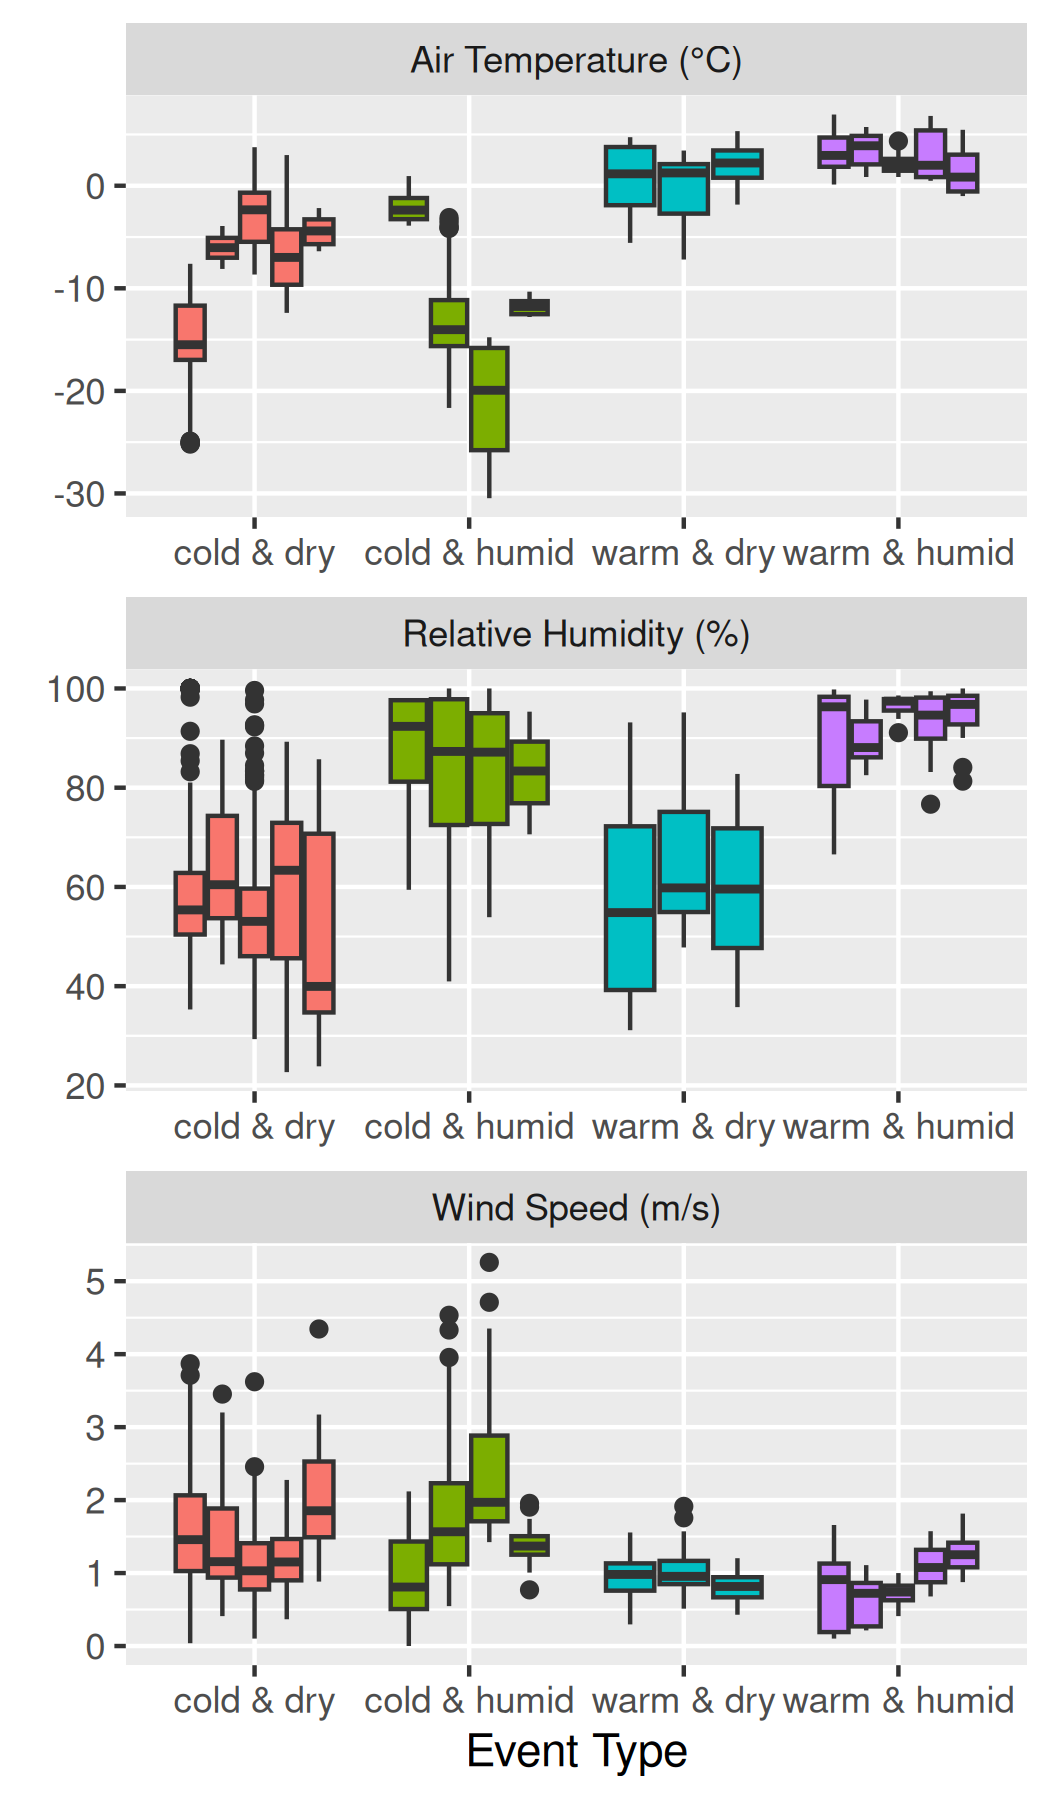
\includegraphics[width=\linewidth,height=0.65\textheight,keepaspectratio]{chapters/04-ablation-paper/figs/figure8.png}

}

\caption{\label{fig-event-met-boxplot}Boxplots showing the distribution
of meteorological measurements of air temperature, relative humidity,
and wind speed over each of the seventeen select ablation events. Air
temperature, relative humidity, and wind speed were measured at FT
station. Note: the rectangle vertical extent represents the
interquartile range (25\textsuperscript{th} to 75\textsuperscript{th}
percentile), the horizontal line within each box indicates the median,
and the whiskers extend to 1.5 times the interquartile range. Circular
points beyond the whiskers represent outliers.}

\end{figure}%

Simulated canopy snow load by the CP25 model closely matched the
observations for all 17 events, demonstrating the most consistent
agreement amongst the models evaluated
(Figure~\ref{fig-obs-mod-w-tree}). The large declines in canopy snow
load for E10 (Figure~\ref{fig-obs-mod-w-tree}) are due to the maximum
canopy snow load used in this model which ranged from 7 to 12 mm
depending on the fresh snow density (a function of air temperature in
Hedstrom \& Pomeroy, 1998).

The energy balance-based snowmelt modelling approaches (CP25 \& SA09)
yielded the most accurate representation of canopy snowmelt over the
warm \& humid events. The CP25 mean bias of 0.02 mm
hr\textsuperscript{-1}, which was smaller than the -0.11 mm
hr\textsuperscript{-1} bias associated with SA09
(Figure~\ref{fig-cpy-load-mb-boxplot}). The improvement for CP25 over
SA09 comes from its representation of the increase in unloading at
higher canopy snow loads (Figure~\ref{fig-unld-melt-ratio}), as observed
for the 2022-06-14 event (Figure~\ref{fig-obs-mod-w-tree}). The air
temperature (R01) and ice-bulb temperature (E10) models produced a wider
range of mean biases (Figure~\ref{fig-cpy-load-mb-boxplot}) and larger
mean bias of over 0.42 mm hr\textsuperscript{-1} during the warm \&
humid events, compared to CP25 and SA09. The rate of ablation was slower
for canopy snow loads below \textasciitilde1.5 mm and \textasciitilde0.3
mm for CP25 and SA09 respectively; due to their differing liquid water
storage capacities (Figure~\ref{fig-obs-mod-w-tree}). For the warm
events other than 2022-04-23, the observed decline in ablation rate
occurs around 2 to 3 mm, exceeding the threshold predicted by all
models.

The warm \& dry events had consistent performance with mean biases of
0.02 mm hr\textsuperscript{-1} for each of the four models
(Figure~\ref{fig-cpy-load-mb-boxplot}). Initiation of ablation was
delayed compared to observations from the weighed tree for the CP25 and
SA09 models for all three of the warm \& dry events
(Figure~\ref{fig-obs-mod-w-tree}). The temperature threshold methods
(E10 \& R01) achieved better timing on the onset of ablation for two
events (2022-03-29 and 2022-04-21) compared to CP25. However, E10
initiated the onset of ablation slightly earlier for 2022-04-23 and the
rate of ablation was also lower than observed for this event.

\begin{figure}

\centering{

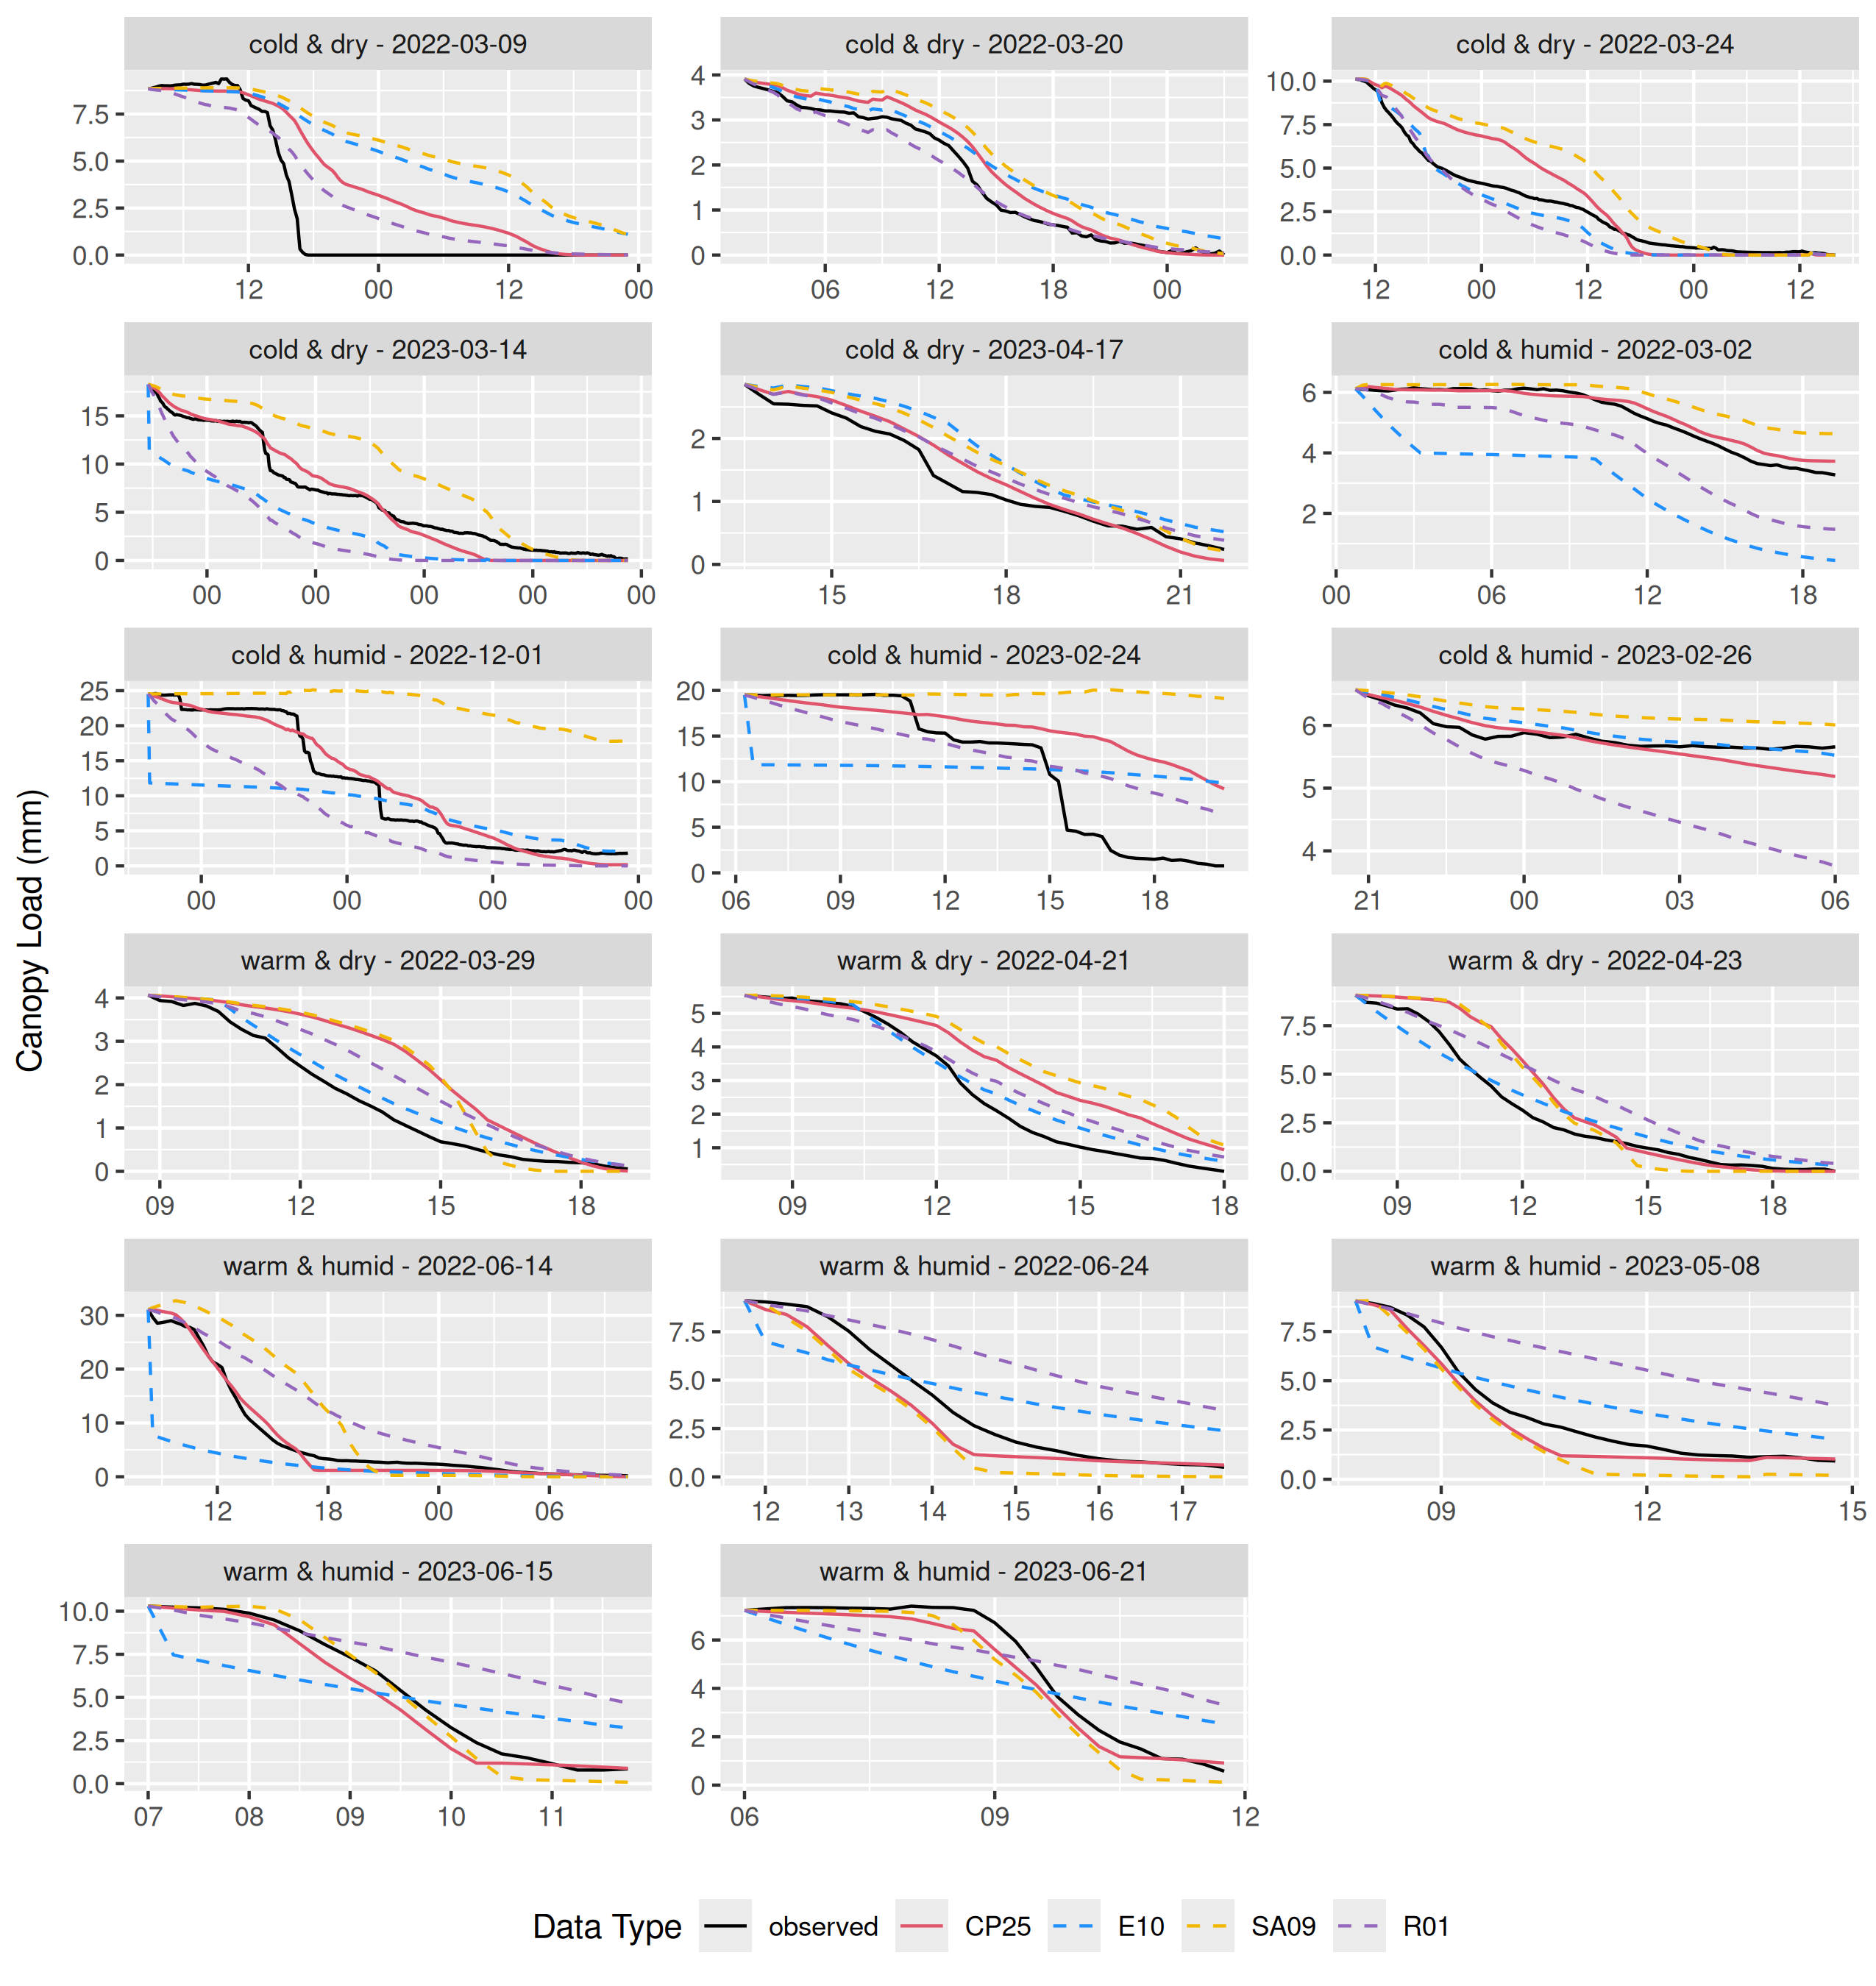
\includegraphics[width=1\linewidth,height=\textheight,keepaspectratio]{chapters/04-ablation-paper/figs/figure9.png}

}

\caption{\label{fig-obs-mod-w-tree}Time series of canopy snow load for
individual events measured by the weighed tree (observed) and simulated
using the four canopy snow models.}

\end{figure}%

For the cold \& dry events, all models had accurate performance with
mean biases ranging from -0.01 to 0.01 mm hr\textsuperscript{-1}, with a
slight improvement in the mean bias for CP25 of -0.009 mm
hr\textsuperscript{-1} (Figure~\ref{fig-cpy-load-mb-boxplot}). Canopy
snowmelt was overestimated by the E10 model and caused the steep initial
decline in canopy snow load on 2022-03-02 which is not registered by the
weighed tree or other models. However, underestimates of ablation
compensated for this overestimate over the remaining cold \& dry
events---which had moderate wind speeds---as wind-driven unloading is
not included in the E10 model (Figure~\ref{fig-event-met-boxplot}). For
events 2022-03-02 and 2023-03-14 the R01 model overestimated canopy snow
ablation due to an overestimation of wind-driven unloading
(Figure~\ref{fig-obs-mod-w-tree}).

The importance of representing wind-driven unloading was clear during
the cold \& humid events, where the mean bias of models including this
mechanism was reduced compared to other approaches; for example, 0.04 mm
hr\textsuperscript{-1} for R01 and 0.15 mm hr\textsuperscript{-1} for
CP25. In contrast, simulations that did not explicitly account for
wind-driven unloading exhibited higher biases, exceeding 0.32 mm
hr\textsuperscript{-1} (Figure~\ref{fig-cpy-load-mb-boxplot}). Although
the E10 model does not include wind-driven unloading, it performed best
for the 2023-02-26 event due to its relatively slow time-based unloading
rate compared to CP25 and R01 which overestimate ablation for this event
(Figure~\ref{fig-obs-mod-w-tree}). The R01 model overestimated unloading
over most of the cold \& humid events and had a higher median bias for
the cold \& humid events compared to CP25
(Figure~\ref{fig-cpy-load-mb-boxplot}). The CP25 model had consistently
lower bias across the three cold \& humid events, but still
underestimated ablation for the 2023-02-24 event which had peak wind
speeds of over 5 m s\textsuperscript{-1}. Over this event, 1.3 mm of
snow was measured at a shielded precipitation gauge in a nearby clearing
and was likely derived from wind transport of snow from the canopy, as
clear skies with no precipitation were observed. The amount of snow
observed to unload from the canopy into the subcanopy lysimeters during
this event was consistent with simulated unloading in CRHM suggesting
that the remaining unaccounted-for snow was likely entrained into the
atmosphere and sublimated and/or transported to distant sites.

\begin{figure}

\centering{

\pandocbounded{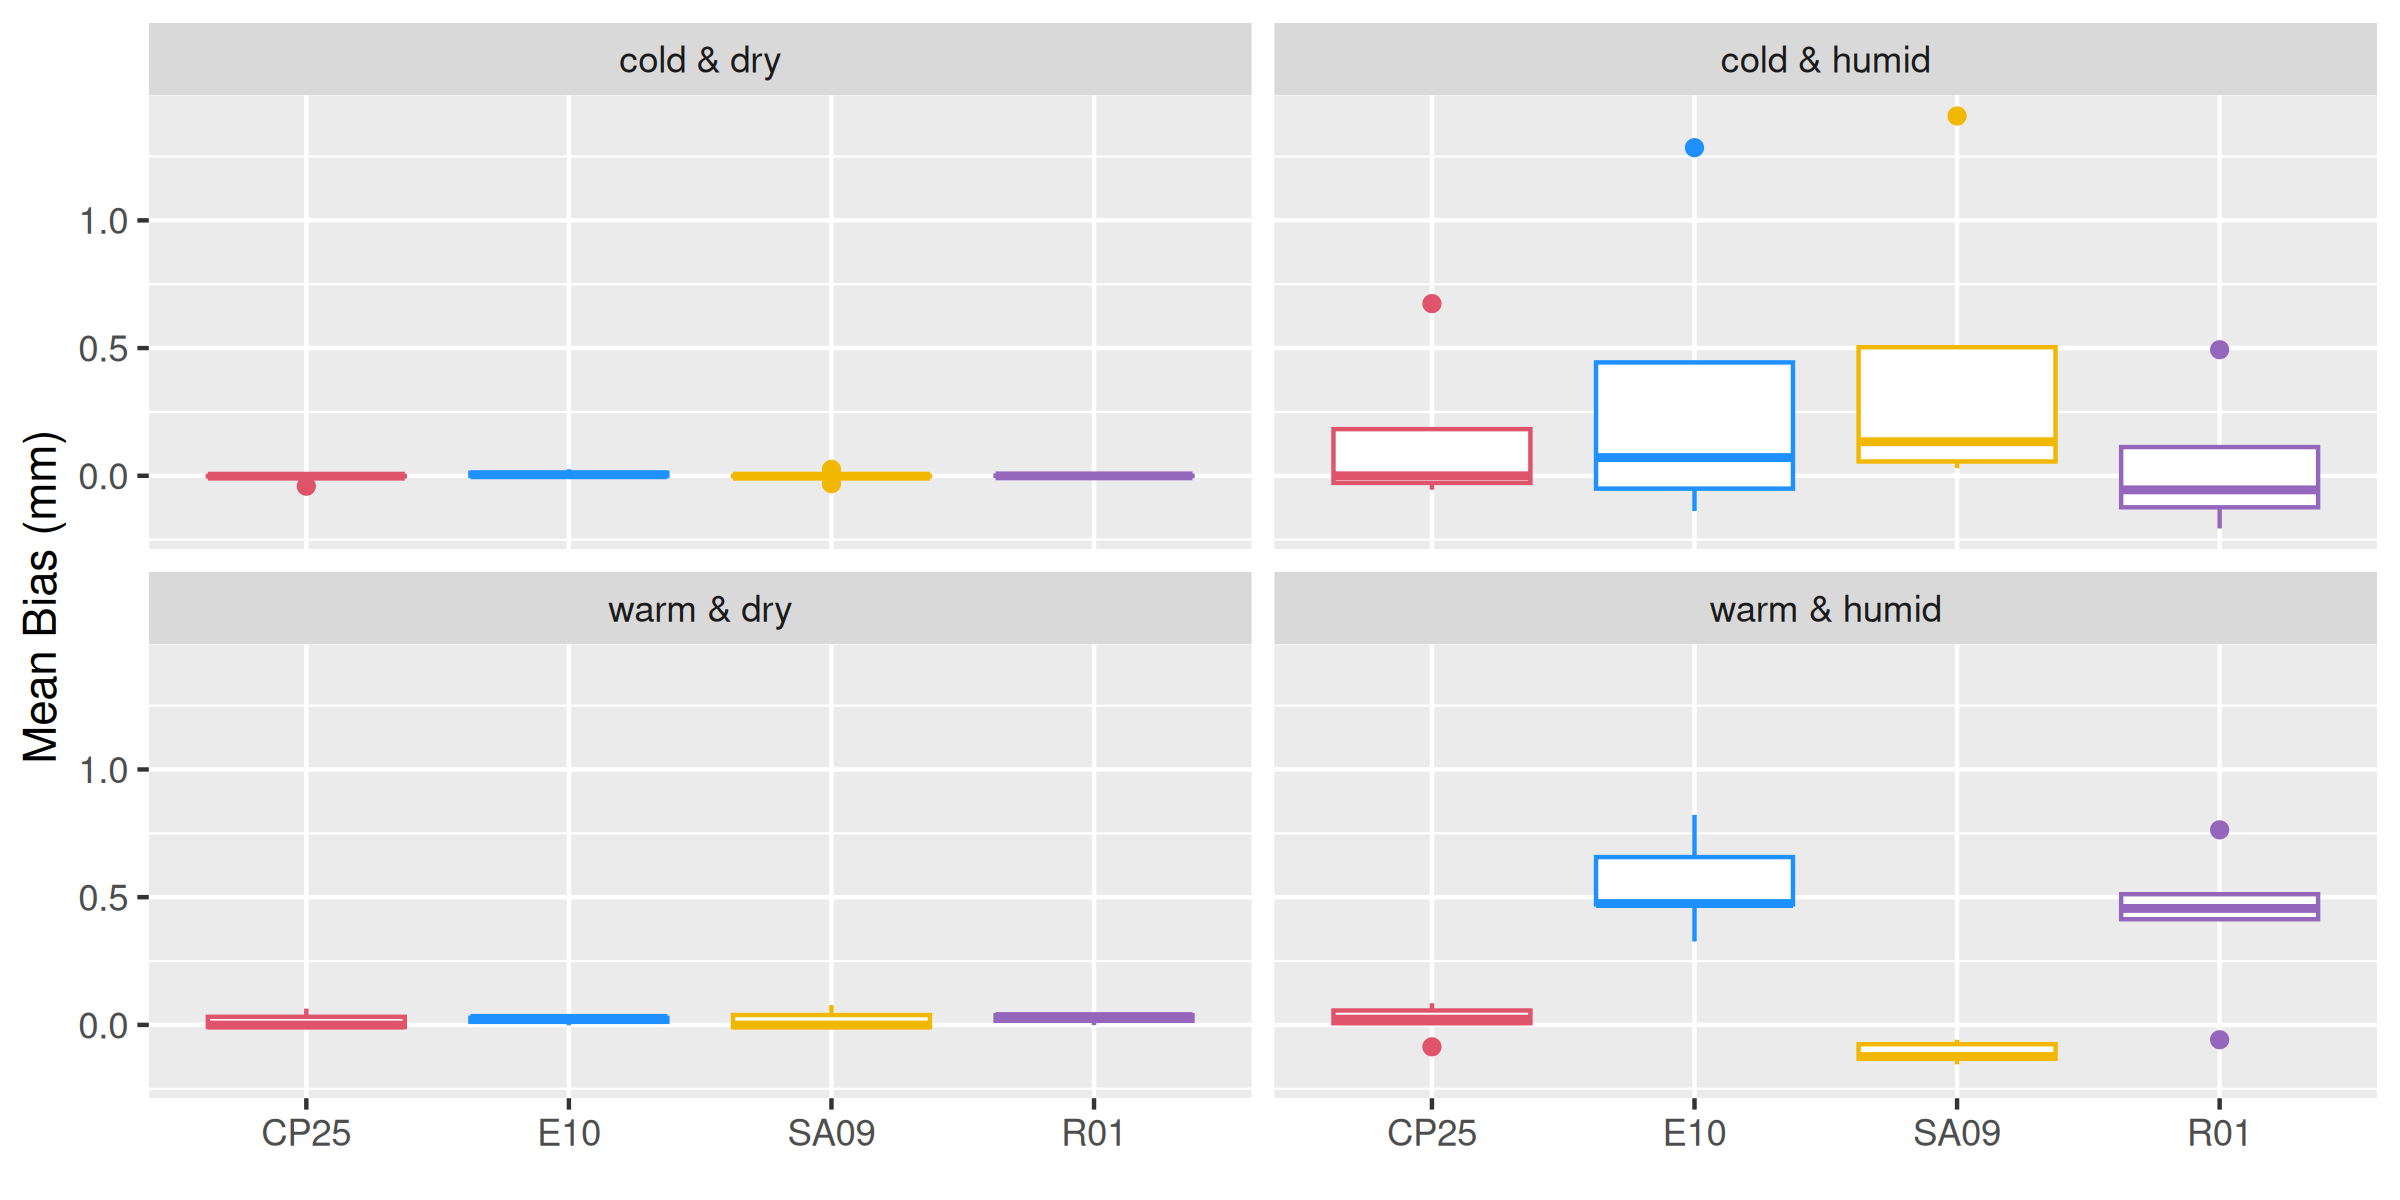
\includegraphics[keepaspectratio]{chapters/04-ablation-paper/figs/figure10.png}}

}

\caption{\label{fig-cpy-load-mb-boxplot}Boxplots illustrating the
distribution of event mean biases calculated between simulations of
canopy snowload and observations from the weighed tree. The vertical
extent of each rectangle represents the interquartile range
(25\textsuperscript{th} to 75\textsuperscript{th} percentile), the
horizontal line within each box indicates the median, and the whiskers
extend to 1.5 times the interquartile range. Circular points beyond the
whiskers represent outliers. The diamonds represent the mean of the
event biases.}

\end{figure}%

\subsection{Canopy Snow Partitioning}\label{canopy-snow-partitioning}

During warm \& humid events, all four parameterisations showed
relatively consistent partitioning of canopy snow, with only a small
fraction returned to the atmosphere (Figure~\ref{fig-partitioning}). The
warm \& dry events had greater variability in the partitioning of
intercepted snow---when compared to the warm \& humid events---with a
larger contribution from sublimation and evaporation processes.
Increased unloading from the E10 model resulted in a greater fraction of
intercepted snow reaching the ground compared to the CP25 model over the
warm \& dry events.

For the cold \& dry and cold \& humid events, the two parameterisations
that include wind-driven unloading (R01 and CP25) had differing
fractions of snow partitioned to the ground via unloading. A higher
fraction of intercepted snow reached the ground for R01 due to the
higher dry snow unloading rate compared to CP25 over all of the cold
events. For both the cold \& dry and cold \& humid events SA09
partitioned all snow back to the atmosphere via sublimation as dry snow
unloading is not included in this parameterisation. Although CP25 and
E10 include differing unloading processes, when averaged over all
events, both had a similar fraction of snow reaching the ground (70\%)
versus the atmosphere (30\%) (Table~\ref{tbl-frac-atm-ground}). SA09 has
the largest discrepancy which returned 40\% of intercepted snow back to
the atmosphere and the R01 with the least amount of snow reaching the
atmosphere with 24\%.

\begin{figure}

\centering{

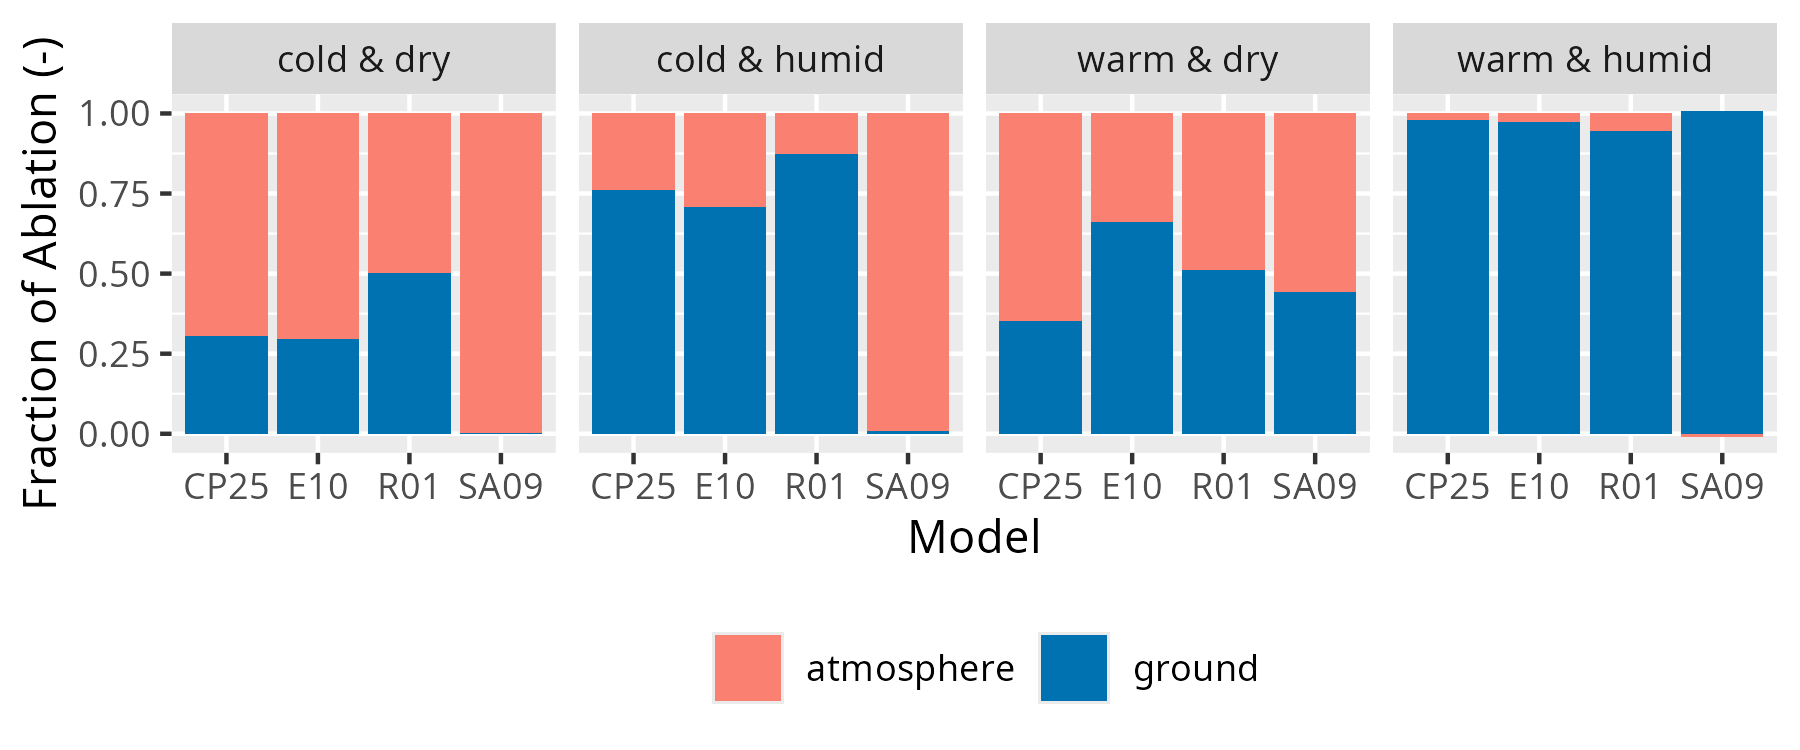
\includegraphics[width=1\linewidth,height=\textheight,keepaspectratio]{chapters/04-ablation-paper/figs/figure11.png}

}

\caption{\label{fig-partitioning}Bar chart illustrating the proportion
of intercepted snow that was either lost to the atmosphere as
sublimation and/or evaporation of melted snow or transferred to the
ground through unloading or drip of melted snow by each event type for
all 17 events.}

\end{figure}%

\begin{longtable}[]{@{}lrr@{}}

\caption{\label{tbl-frac-atm-ground}Fraction of canopy-intercepted snow
returned to the atmosphere as sublimation and evaporation of melted snow
or input to the ground as unloading or drip of melted snow for each
parameterisation over the 17 select ablation events.}

\tabularnewline

\toprule\noalign{}
Model & Atmosphere (-) & Ground (-) \\
\midrule\noalign{}
\endhead
\bottomrule\noalign{}
\endlastfoot
CP25 & 0.29 & 0.71 \\
E10 & 0.31 & 0.69 \\
R01 & 0.24 & 0.76 \\
SA09 & 0.40 & 0.60 \\

\end{longtable}

\section{Discussion}\label{discussion-2}

\subsection{Processes Governing Canopy Snow
Unloading}\label{processes-governing-canopy-snow-unloading}

Observations of canopy snow unloading support the hypothesis that
unloading is primarily controlled by snowmelt and dry-snow related
processes, both of which are also influenced by the amount of snow
intercepted in the canopy (Table~\ref{tbl-q-unld-bins}). The ratio of
unloading to canopy snowmelt was found to increase linearly with
increasing canopy snow load (Figure~\ref{fig-unld-melt-ratio}), which
differs from Storck et al. (2002) who originally found the ratio of
canopy snow unloading to melt to be constant at 0.4. The measurement
difficulties noted by Storck et al. (2002) limited their estimate of
this ratio to a single mid-December event, preventing any association
with canopy snow load. Similar instrument difficulties here in measuring
canopy snowmelt drainage limited direct measurements to three events and
hybrid measurements (from Equation~\ref{eq-unld-melt-mass-bal}) to 5
events (Figure~\ref{fig-unld-melt-ratio}). The reasonable correspondence
between observed and modelled canopy snow drip for these events supports
the linear increase hypothesis (Figure~\ref{fig-cml-tb}). Previous
studies have identified relationships between melt-induced unloading and
various meteorological parameters, including empirical functions of air
temperature (Katsushima et al., 2023; Roesch et al., 2001), ice-bulb
temperature (Ellis et al., 2010; Floyd, 2012), and solar radiation
(Katsushima et al., 2023). Although branch bending and subsequent
unloading has been shown to be associated with air temperature (Schmidt
\& Gluns, 1991; Schmidt \& Pomeroy, 1990), observations here indicate
that temperature-related unloading increases occur primarily near the
freezing point (Figure~\ref{fig-q-unld-all-bins}), eliminating the need
for a separate temperature parameterisation beyond snowmelt-associated
unloading processes.

Dry snow unloading was found to increase exponentially with wind speed
and linearly with shear stress (Table~\ref{tbl-q-unld-wind}). These
results differ from earlier research that has represented this process
as a linear function of wind speed and canopy load (Bartlett \&
Verseghy, 2015; Katsushima et al., 2023; Roesch et al., 2001), as shown
in Figure~\ref{fig-unl-ex-wind}. The higher \emph{R\textsuperscript{2}}
found for shear stress compared to wind speed for predicting
unloading---when excluding melt events---is likely due to the physical
relationship between shear stress force and kinetic energy transfer to
the canopy, wind transport from the canopy, and movement of branches in
the canopy induced by drag (shear) forces. The differing relationship
presented here, compared to the R01 model
(Figure~\ref{fig-unl-ex-wind}), may be attributed to the development of
that parameterisation using above canopy albedo as a proxy for canopy
snow unloading (Bartlett \& Verseghy, 2015; Roesch et al., 2001). This
approach would have included both unloading and sublimation processes,
in addition to greater measurement uncertainties (Cebulski \& Pomeroy,
2025a). Conversely, the subcanopy lysimeter measurements employed here
provided a more direct quantification of canopy snow unloading rates.
Simulated unloading over events classified as cold \& humid---which had
the largest contribution of wind-driven unloading---resulted in the
highest overall mean biases compared to the warm \& dry, warm \& humid,
and cold \& dry events (Figure~\ref{fig-cpy-load-mb-boxplot}).
Additional factors that may influence dry snow unloading that are not
considered in the new parameterisation (Equation~\ref{eq-q-unld-wind})
include wind erosion, branch movement, structural degradation, bond
weakening, increased elasticity of branches, snow density, and liquid
water content. The addition of liquid water content in the canopy snow
due to phase change can increase cohesion and adhesion of snow clumps
within the canopy (Pomeroy \& Gray, 1995). However, high liquid water
contents during rapid melt can lubricate the snow attachment to the
canopy and weaken cohesive bonds, inducing unloading, much as for wet
snow avalanches (Baggi \& Schweizer, 2008).

The density of snow intercepted in the canopy is expected to influence
both dry snow and melt-induced unloading processes---and is incorporated
in the E10 parameterisation for the initial accumulation component based
on the findings of Schmidt \& Gluns (1991)---but is not explicitly
represented in any of the ablation calculations included in this study.
Fresh, low-density snow typically exhibits lower cohesion and adhesion
compared to older snow, which may have undergone freeze-thaw cycles or
equitemperature metamorphism, processes that increase snow density and
bond strength hence, increasing the mechanical resistance to unloading.
While vapour deposition and rime-ice accumulation are simulated in some
models (e.g., Clark et al., 2015b; Ellis et al., 2010) via the latent
heat flux parameterisation, they are usually treated as additions to the
canopy snow reservoir. However, in humid or maritime regions rime can
form dense, ice-like structures (e.g., Berndt \& Fowler, 1969) with high
resistance to unloading by either melt or wind (Lumbrazo et al., 2022).
Although canopy snow density is expected to influence ablation
processes, it was not observed in this study due to its continental
location and remains a research gap for maritime climates.

The relationship between unloading and canopy snow sublimation was not
statistically significant (Figure~\ref{fig-q-unld-all-bins}). This
differs from earlier work by MacDonald (2010) who found an association
between these two variables and attributed this to the reduction in
structural integrity and bond weakening of the canopy snow clumps as
snow particles are removed through sublimation. It is possible that the
association identified by MacDonald (2010) arose from the concurrent
increase in canopy energy inputs that promote both sublimation and other
ablation mechanisms such as melt and other dry snow unloading processes
which were not directly accounted for.

\subsection{Performance Comparison of Ablation
Models}\label{performance-comparison-of-ablation-models}

The improved performance of the new CP25 model across a wide range of
meteorological conditions demonstrates the advantages of incorporating
comprehensive snow unloading processes coupled with physically based
representations of the energy balance to simulate ablation
(Figure~\ref{fig-obs-mod-w-tree}). In contrast, existing models were
limited by missing processes such as wind-driven unloading (SA09 and
E10) or relied on temperature-dependent parameterisations of melt and
drip processes which had limited transferability across differing events
(R01 and E10). Although the SA09 model---originally developed in a
relatively warm maritime climate with limited wind influence (Storck et
al., 2002)---performed similarly well to CP25 during most of the
melt-dominated events, its exclusion of wind-induced unloading led to
poor performance for the cold \& dry and cold \& humid events. This
process omission caused SA09 to overestimate sublimation when averaged
over all events (Table~\ref{tbl-frac-atm-ground}). Moreover, the
constant canopy snow unloading to melt ratio of 0.4 in the SA09 model
led to reduced performance for one melt event with canopy snow loads up
to 30 mm, whereas the CP25 model more accurately predicted ablation over
this event. The low liquid water retention capacity implemented in SA09
also contributed to an underestimation of canopy loads during the end of
most melt events (Figure~\ref{fig-obs-mod-w-tree}).

Models utilising temperature-based canopy snowmelt parameterisations
(E10 and R01) exhibited inconsistent performance, particularly during
warm \& humid events where they underestimated ablation. This was due to
their reliance on air temperature or ice-bulb temperature as proxies for
energy input into the canopy, which failed to represent the energy
availability over these events. In contrast, all four models performed
similarly during warm \& dry events, where air temperatures were closer
to 0°C. The superior performance of the energy balance-based canopy
snowmelt models (CP25 and SA09) during warm \& humid events likely
reflects their ability to represent the elevated energy inputs which
were present over the warmer events.

While E10 omitted any explicit representation of wind-driven unloading,
its exponential time decay parameterisation indirectly addressed this
process, though it still underestimated overall ablation for the cold
events which had higher wind speeds (Figure~\ref{fig-obs-mod-w-tree}).
The maximum canopy snow load threshold implemented in the E10 model was
lower than observations from the weighed tree. This limitation offset
its tendency to underestimate unloading processes as was also observed
by Lundquist et al. (2021) and Lumbrazo et al. (2022). In this study,
the CP25, SA09, and R01 models did not include a maximum snow load, and
their performance aligns with the hypothesis of Lundquist et al. (2021)
that this limit may be unnecessary---or much higher than previously
though---when combined with a comprehensive canopy snow ablation
routine. In contrast, R01 consistently overestimated wind-driven
unloading during both the cold \& dry and cold \& humid events,
potentially due to the differing methodology used to develop this
parameterisation (Figure~\ref{fig-obs-mod-w-tree}). CP25 provided a
better representation of wind-driven unloading compared to R01 aside
from one one event with high wind speeds (\textgreater5 m
s\textsuperscript{-1})---that cause wind redistribution/entrainment of
snow into the atmosphere. Wind unloading parameters also may be
influenced by tree species, forest structure, and snow characteristics
(Lumbrazo et al., 2022), necessitating further field-based research on
canopy snow unloading in diverse environments to assess their broader
applicability.

The infrequent occurrence of wind-transport from the canopy in our
observations may account for underestimation of ablation during one
strongly wind-dominated events by CP25 (2023-02-24,
Figure~\ref{fig-obs-mod-w-tree}). Wind transport of canopy snow to the
nearby Powerline snowfall gauge occurred during this event, but was a
small fraction of canopy snow ablation, 1.3 mm of a total of 20 mm of
canopy snow ablation. Since unloading measured by the subcanopy
lysimeters corresponded well with CP25 predictions for this event, the
approximately 9 mm of unaccounted canopy snow ablation may be attributed
to uncertainties within the wind-driven unloading parameterisation
(Figure~\ref{fig-q-unld-wind}) and possible atmospheric entrainment of
canopy snow that was either transported to distant locations and/or
sublimated. These findings align with observations by Troendle (1983)
but contrast with Hoover \& Leaf (1967), who proposed that most
wind-transported snow relocates to nearby sites with minimal sublimation
effects.

\subsection{Canopy Snow Partitioning}\label{canopy-snow-partitioning-1}

Substantial variability was found in the fraction of snow that
sublimated and/or evaporated as liquid meltwater versus unloading and
drip depending on the canopy snow ablation model selected
(Figure~\ref{fig-partitioning}). For example, the exclusion of
wind-driven unloading processes in the SA09 model resulted in 100\% of
intercepted snow reaching the atmosphere for both the cold \& dry and
cold \& humid events. This differed considerably from the CP25 model
which returned 70\% and 24\% of snow back to the atmosphere for the cold
\& dry and cold \& humid events, respectively. Although E10 and CP25
include differing process representations, they predicted comparable
fractions of snow reaching the ground versus returning to the
atmosphere. The agreement between CP25 and E10 is notable, since the E10
has been tested and found to perform well in predicting subcanopy
snowpacks around the world (Ellis et al., 2010; Gelfan et al., 2004;
Pomeroy et al., 2022; Sanmiguel-Vallelado et al., 2022b). However, the
results shown here reveal that E10's individual process representations
can be in error, particularly under warm and windy conditions,
potentially explaining the difficulties when applying E10 at locations
where parameterisation errors fail to offset one another (Lumbrazo et
al., 2022; Lundquist et al., 2021). For example, at locations which
intercept a larger amount of snow, the E10 maximum canopy snow load
would overestimate the amount of unloading, and a greater deviation
between the E10 and CP25 model is expected.

\subsection{Future Directions}\label{future-directions}

Physically based approaches such as CP25 are particularly relevant for
predictions of snow hydrology under a changing climate, where warming
may reduce the reliability of empirically derived canopy snowmelt models
like E10 and R01. The improved representation of melt events by CP25 and
SA09 demonstrates the reliability of more physically based methods
across a range of meteorological conditions, compared to
temperature-based canopy snowmelt routines (E10 and R01) which had
reduced performance over these events. Amongst all canopy snow ablation
processes, dry snow unloading introduced the most uncertainty. Although
the revised model performed best for this dataset, further validation is
required across a wider range of climates and forest structures. Since
unloading, melt, and sublimation are competitive ablation processes,
they strongly influence whether snow is returned to the atmosphere or
reaches the ground.

Key limitations remain in measuring canopy snow sublimation using eddy
correlation systems (Conway et al., 2018; Harding \& Pomeroy, 1996;
Harvey et al., 2025; Helgason \& Pomeroy, 2012b; Parviainen \& Pomeroy,
2000) and separating snow unloading from meltwater drip (Floyd, 2012;
Storck et al., 2002), which limit the development and testing of canopy
snow ablation parameterisations. Whilst separating initial interception
and ablation processes (Cebulski \& Pomeroy, 2025a; Cebulski \& Pomeroy,
2025b), will improve process representations, these routines still need
to be evaluated together against additional field observations.
Incorporating the updated unloading schemes developed here could improve
the representation of canopy snow ablation and, by extension, the
partitioning of precipitation and canopy albedo in hydrological and land
surface models. Nonetheless, further testing is needed across different
sites, climates, forest types, and spatial scales to assess model
transferability and performance.

\section{Conclusions}\label{conclusions-2}

Canopy snow ablation processes govern the timing and partitioning of
snowfall to the ground versus the atmosphere in forested environments,
yet their representation in modelling frameworks remains uncertain due
to insufficient process-level validation. This study evaluates existing
canopy snow ablation theories using in-situ measurements of canopy snow
load, unloading, and drip combined with a novel canopy snow energy and
mass balance model. These observations revealed that canopy snow load,
wind shear stress, and canopy snowmelt were statistically significant
predictors of snow unloading, collectively explaining 80\% of its
variability. In addition to this empirical evidence, physical processes
such as structural degradation, snow particle bond weakening,
lubrication of wet canopy snow during melt, and the shear force exerted
on canopy snow by wind further support representing these processes.
Although some studies use air temperature as an index of unloading
resulting from canopy snowmelt and potential branch bending, here energy
balance methodologies show improved performance in simulating canopy
load during melt events.

Previous studies have demonstrated relationships between unloading and
snow load, wind speed, and canopy snowmelt rate, but these processes
have not been evaluated collectively. This study represents the first
development and validation of an unloading model addressing both energy
balance-based melt and dry snow unloading processes together. Novel
parameterisations for dry snow and melt-induced unloading were
introduced, with key differences from previously established approaches.
Shear stress was found to be a stronger predictor of dry snow unloading
(\emph{R\textsuperscript{2}} = 0.61) than wind speed
(\emph{R\textsuperscript{2}} = 0.54) for non-melt periods. The canopy
melt rate exerted the strongest control on snow unloading during melt
events, consistent with one existing model. A new finding was that the
ratio of unloading to canopy snowmelt increased with canopy snow load.
Additionally, an existing approach which used the concept of a maximum
intercepted snow load greatly underestimated the canopy snow storage
capacity when compared to observed snow loads from weighed tree
measurements. Throughout the two-years of observations presented here, a
maximum canopy snow load was not observed, likely as unloading rates
increased with higher snow loads. Wind transport events were relatively
rare in this wind-exposed subalpine forest, but resulted in a
considerable underestimation of the amount of snow returned to the
atmosphere or surrounding sites during one event.

A new canopy snow ablation model that integrates an updated canopy snow
mass and energy balance demonstrated improved accuracy across varied
meteorological conditions compared to existing approaches. Existing
models failed to maintain accuracy across events with a wide range of
meteorology due to neglect of key processes and/or empirical
representations of melt processes. The greatest inter-model
discrepancies in canopy snow load occurred during warm and humid events,
where temperature-based canopy snowmelt parameterisations showed
substantially higher mean biases relative to energy balance-based
models.

Amongst the models tested, the largest errors were found during cold \&
dry unloading events---though performance was improved when
incorporating a site-specific shear stress-based parameterisation.
Partitioning of intercepted snow disposition between the ground and
atmosphere varied most amongst cold events, where neglecting the dry
snow unloading process resulted in considerable overestimates of canopy
snow sublimation losses. All canopy snow models had greater consistency
in partitioning canopy snow during warm \& humid events, where all
canopy snow was typically unloaded or melted as drip towards the ground
surface. However, the rate of unloading was best represented by energy
balance-based canopy snowmelt routines compared to empirical
relationships. Although improved performance was found for the updated
canopy snow ablation model compared to existing methods, across a wide
range of meteorological conditions, additional testing across various
climate and forest compositions is required to assess model
transferability.

\section{Acknowledgements}\label{acknowledgements}

We acknowledge financial support from the University of Saskatchewan
Dean's Scholarship, the Natural Sciences and Engineering Research
Council of Canada's Discovery Grants, the Canada First Research
Excellence Fund's Global Water Futures Programme, Environment and
Climate Change Canada, Alberta Innovates Water Innovation Program, the
Canada Foundation for Innovation's Global Water Futures Observatories
facility, and the Canada Research Chairs Programme. We thank Madison
Harasyn, Hannah Koslowsky, Kieran Lehan, Lindsey Langs and Fortress
Mountain Resort for their help in the field and Tom Brown and Logan Fang
for support of the CRHM platform.

\section{Data \& Software Availability
Statement}\label{data-software-availability-statement}

The Cold Regions Hydrological Model Platform (CRHM) source code is
available at https://github.com/srlabUsask/crhmcode. Model forcing data,
model outputs, validation data, processed data, and scripts are
available at https://doi.org/10.5281/zenodo.16898881.

\pagebreak

\bookmarksetup{startatroot}

\chapter{Evaluation of a New Needleleaf Forest Snowpack Model for
Diagnosing Snow Accumulation Regimes in Western and Northern
Canada}\label{evaluation-of-a-new-needleleaf-forest-snowpack-model-for-diagnosing-snow-accumulation-regimes-in-western-and-northern-canada}

Manuscript status: Analysis is complete and manuscript is currently in
progress. Anticipated submission is to the journal \emph{Hydrological
Processes} Fall, 2025.

Citation: Cebulski, A. C., Pomeroy, J. W., Floyd, W. C. (in prep.).
Evaluation of a New Needleleaf Forest Snowpack Model for Diagnosing Snow
Accumulation Regimes in Western and Northern Canada. \emph{Hydrological
Processes}, 12, e70010. https://doi.org/10.1002/wat2.70010

Role in thesis: This journal article corresponds to research question
2.1 of the thesis, the model implementation and testing phase. New
parameterisations and process understanding of snow interception and
ablation processes from chapters 1, 2 and 3 will incorporated into the
Cold Regions Hydrological Model (CRHM) platform to model forest snow
accumulation at four research basins in western Canada. The updated
parameterisations will be evaluated by including them in an updated CRHM
canopy module. Simulated SWE using this updated module will be compared
to observed SWE at a point within the forest of each research basin.

\section{Abstract}\label{abstract-3}

\section{Introduction}\label{introduction-4}

Snow is an important water resource, directly supporting over two
billion people globally (Immerzeel et al., 2020; Viviroli et al., 2020),
while also affecting earths energy balance via surface albedo (Thackeray
et al., 2014; Wang et al., 2016) and stream temperatures (e.g., Leach \&
Moore, 2014). However, snowpacks are increasingly threatened due to
changes in both climate and vegetation cover worldwide (Immerzeel et
al., 2020; López-Moreno et al., 2014; Viviroli et al., 2020). In
cold-dry climates, sublimation of snow intercepted by forest canopies
can return up to 45\% of seasonal snowfall back to the atmosphere
(Essery et al., 2003; Sanmiguel-Vallelado et al., 2017), whereas in
temperate-maritime climates sublimation is less prevalent and a large
fraction of snowfall melts in the canopy (Storck et al., 2002).
Hydrological models are essential tools for understanding how climate
and vegetation influence snow processes and downstream water resources,
and their accuracy depends on accurate representations of forest-snow
processes. Yet, uncertainties in forest-snow process representation lead
to variable transferability across climates and forest types when
simulating subcanopy snow water equivalent (SWE) (Essery et al., 2003;
Gelfan et al., 2004; Krinner et al., 2018; Rutter et al., 2009) and
diagnosing snow processes (Lumbrazo et al., 2022; Lundquist et al.,
2021). This variability is compounded by the strong dependence of snow
partitioning by vegetation on meteorology and canopy density which has
challenged earlier canopy snow parameterisations that have been tested
and developed on sparse observations (Lundquist et al., 2021). Over half
of the Northern Hemisphere experiences snowfall in forested areas (Kim
et al., 2017) and over 23\% of land mass globally (Deschamps-Berger et
al., 2025), spanning diverse climates and forest structures,
highlighting the need for robust models, transferable models. While
simulation of SWE in forests remains challenging it is a crucial aspect
to understand the impacts of climate and land cover changes on water
resources in many cold regions across the globe.

Recent studies have advanced understanding of the canopy snow energy and
mass balance (Cebulski \& Pomeroy, 2025b; Cebulski \& Pomeroy, 2025c;
Lumbrazo et al., 2022; Lundquist et al., 2021), with potential to
improve SWE simulations in forested basins. For example, Lundquist et
al. (2021) demonstrated that calculating throughfall as a function of
antecedent snow load can overestimate snow reaching the ground---when
also combined with a comprehensive canopy snow unloading routine.
Building on this, Staines \& Pomeroy (2023) and Cebulski \& Pomeroy
(2025b) showed that initial interception can predicted as a function of
canopy density without assuming maximum canopy snow load. Moreover,
Roesch et al. (2001) and Lumbrazo et al. (2022) show the importance of
representing both wind and melt-induced unloading for representing
canopy snow ablation. A new physically-based canopy snow mass and energy
balance presented in Cebulski \& Pomeroy (2025c) provided improved
representation of canopy snow ablation compared to previous approaches
that were either missing key processes (i.e., dry snow unloading in
Andreadis et al., 2009) or based on empirical relationships (i.e.,
ice-bulb temperature induced melt unloading and drip in Ellis et al.,
2010). These advances have been implemented as new parameterisations in
the Cold Regions Hydrological Modelling Platform to answer the following
research questions:

\begin{enumerate}
\def\labelenumi{\arabic{enumi}.}
\tightlist
\item
  What is the performance of a novel hydrological model in simulating
  the accumulation of subcanopy SWE in forested environments
  characterized by varying tree species, canopy structures, and
  meteorological conditions?
\item
  How does the performance of the new model in simulating SWE compare to
  that of a conventional modelling approach across differing
  environments?
\item
  What are the canopy snow processes that account for the differences in
  SWE between the modelling approaches and how do these differ with
  climate and forest structural differences?
\end{enumerate}

The objective of this research is to evaluate new snow interception and
ablation parameterizations for simulating subcanopy SWE and diagnosing
causative processes in needleleaf forests. Evaluation of the new model
in simulating initial accumulation of snow in the canopy has been
addressed in Cebulski \& Pomeroy (2025b) and canopy snow ablation in
Cebulski \& Pomeroy (2025c).

\section{Methods}\label{methods-1}

\subsection{Study Sites}\label{study-sites}

The needleleaf snowpack models were evaluated at four locations in
western Canada spanning a range of climate and forest types
(Figure~\ref{fig-map}; Table~\ref{tbl-site-meta}). The model simulation
years for each site are shown in Table~\ref{tbl-site-meta} and were
selected based on the availability of bi-weekly to monthly subcanopy SWE
measurements and hourly station-based observations of air temperature,
relative humidity, wind speed, total precipitation, and net solar
radiation adjacent to the snow survey transects. At each site, snow
surveys consisted of snow depth measurements at all locations and snow
density measurements at one out of every five locations. SWE was
calculated from snow depth and snow density following the methods
outlined in Pomeroy \& Gray (1995). The four study sites include:

Wolf Creek Research Basin - Forest Site (60.60, -134.96, 750 m asl.) is
located 16 km south of Whitehorse, Yukon Territory in a level dense
forest with a sub-arctic climate (see basin scale location in Fig. 1 in
Rasouli et al., 2019a). Snow surveys were conducted along a transect
that traverses through mature forest consisting of primarily White
spruce and Lodgepole pine. Additional details on the snow survey and
meteorological measurements is described in Rasouli et al. (2019a) and
Pomeroy et al. (2025).

Russell Creek Experimental Watershed - Upper Stephanie Old Growth Site
(50.32, -126.35, 700 m asl.) is located on northern Vancouver Island,
British Columbia with a temperate-maritime climate that receives
substantial winter precipitation. Snow survey transects were conducted
in cardinal directions within a mature old growth forest that consists
of Amabilis fir and Western hemlock (Floyd, 2012). Additional details on
the snow survey and meteorological instrumentation are provided in Floyd
(2012). Total precipitation data were unavailable at the Russell site
for the 2008 water year. For this period, records from the Tsitika
Summit station (50.28°N, 126.36°W; 450 m asl.), operated by the British
Columbia Ministry of Transport and located 5 km from Russell, were used
instead.

Fortress Mountain Research Basin - Powerline site (50.83, -115.20, 2100
m asl., Kananaskis, Alberta) is located on a wind-exposed subalpine
ridge top covered with sparse forest with a continental climate (see
basin scale location in Fig. X in Pomeroy et al., 2025). The vegetation
at this site consists of coexisting Subalpine fir and Engelmann spruce
tree species (Langs et al., 2020). Snow survey measurements of snow
depth and density were collected following a transect through mature
forest east of the Powerline meteorological tower (see Fig. 1 in
Cebulski \& Pomeroy, 2025b) and described in further detail in Pomeroy
et al. (2025). The meteorological forcing data used in this study is
described in detail in Cebulski \& Pomeroy (2025c).

Marmot Creek Research Basin - Upper Forest site (50.93, -115.16, 1848 m
asl., Kananaskis, Alberta) is located on a dense forested plateau with a
continental climate 14 km north of Fortress but receives much less
precipitation (see basin scale location in Fig. 1 in Fang et al., 2019).
Vegetation consisted primarily of Engelmann spruce, subalpine fir, and
lodgepole pine (Fang et al., 2019; Staines \& Pomeroy, 2023). Snow
surveys were conducted following a cardinal transect through mature
forest surrounding the ``Upper Clearing'' meteorological tower (see Fig.
1b in Staines \& Pomeroy, 2023) and described in further detail in
Pomeroy et al. (2025). The meteorological forcing data and corresponding
instrumentation used from this site is described in Fang et al. (2019)
and Pomeroy et al. (2025).

\begin{longtable}[]{@{}
  >{\raggedright\arraybackslash}p{(\linewidth - 16\tabcolsep) * \real{0.1100}}
  >{\raggedright\arraybackslash}p{(\linewidth - 16\tabcolsep) * \real{0.0900}}
  >{\raggedleft\arraybackslash}p{(\linewidth - 16\tabcolsep) * \real{0.0900}}
  >{\raggedleft\arraybackslash}p{(\linewidth - 16\tabcolsep) * \real{0.1100}}
  >{\raggedleft\arraybackslash}p{(\linewidth - 16\tabcolsep) * \real{0.0900}}
  >{\raggedleft\arraybackslash}p{(\linewidth - 16\tabcolsep) * \real{0.0900}}
  >{\raggedleft\arraybackslash}p{(\linewidth - 16\tabcolsep) * \real{0.0900}}
  >{\raggedleft\arraybackslash}p{(\linewidth - 16\tabcolsep) * \real{0.0900}}
  >{\raggedright\arraybackslash}p{(\linewidth - 16\tabcolsep) * \real{0.2000}}@{}}

\caption{\label{tbl-site-meta}Simulation period (Years), location, and
vegetation characteristics, including canopy cover (\(C_c\)), leaf area
index (LAI), and mean tree height (\(\overline{h_t}\)), for the four
study sites.}

\tabularnewline

\toprule\noalign{}
\begin{minipage}[b]{\linewidth}\raggedright
Site Name
\end{minipage} & \begin{minipage}[b]{\linewidth}\raggedright
Years
\end{minipage} & \begin{minipage}[b]{\linewidth}\raggedleft
Ele. (m)
\end{minipage} & \begin{minipage}[b]{\linewidth}\raggedleft
Lon.
\end{minipage} & \begin{minipage}[b]{\linewidth}\raggedleft
Lat.
\end{minipage} & \begin{minipage}[b]{\linewidth}\raggedleft
\(C_c\)
\end{minipage} & \begin{minipage}[b]{\linewidth}\raggedleft
LAI
\end{minipage} & \begin{minipage}[b]{\linewidth}\raggedleft
\(\overline{h_t}\) (m)
\end{minipage} & \begin{minipage}[b]{\linewidth}\raggedright
Dominant Species
\end{minipage} \\
\midrule\noalign{}
\endhead
\bottomrule\noalign{}
\endlastfoot
Wolf Creek & 2015---2022 & 750 & -134.96 & 60.60 & 0.81 & 3.82 & 15.0 &
White Spruce and interior lodgepole pine \\
Marmot Creek & 2007---2023 & 1848 & -115.16 & 50.93 & 0.80 & 3.00 & 15.0
& Engelmann spruce, subalpine fir, and lodgepole pine \\
Fortress Mountain & 2013---2023 & 2100 & -115.20 & 50.83 & 0.65 & 1.44 &
10.5 & Subalpine fir and engelmann spruce \\
Russell Creek & 2006---2008 & 700 & -126.35 & 50.32 & 0.86 & 1.93 & 44.9
& Amabilis fir and western hemlock \\

\end{longtable}

\begin{figure}

\centering{

\includegraphics[width=0.8\linewidth,height=\textheight,keepaspectratio]{chapters/05-model-eval-paper/figs/figure1.png}

}

\caption{\label{fig-map}Map showing the regional scale location of the
four research basins and land cover data from the Canada Centre for
Remote Sensing et al. (2020) North American Land Change Monitoring
30-meter dataset.}

\end{figure}%

\begin{figure}

\centering{

\pandocbounded{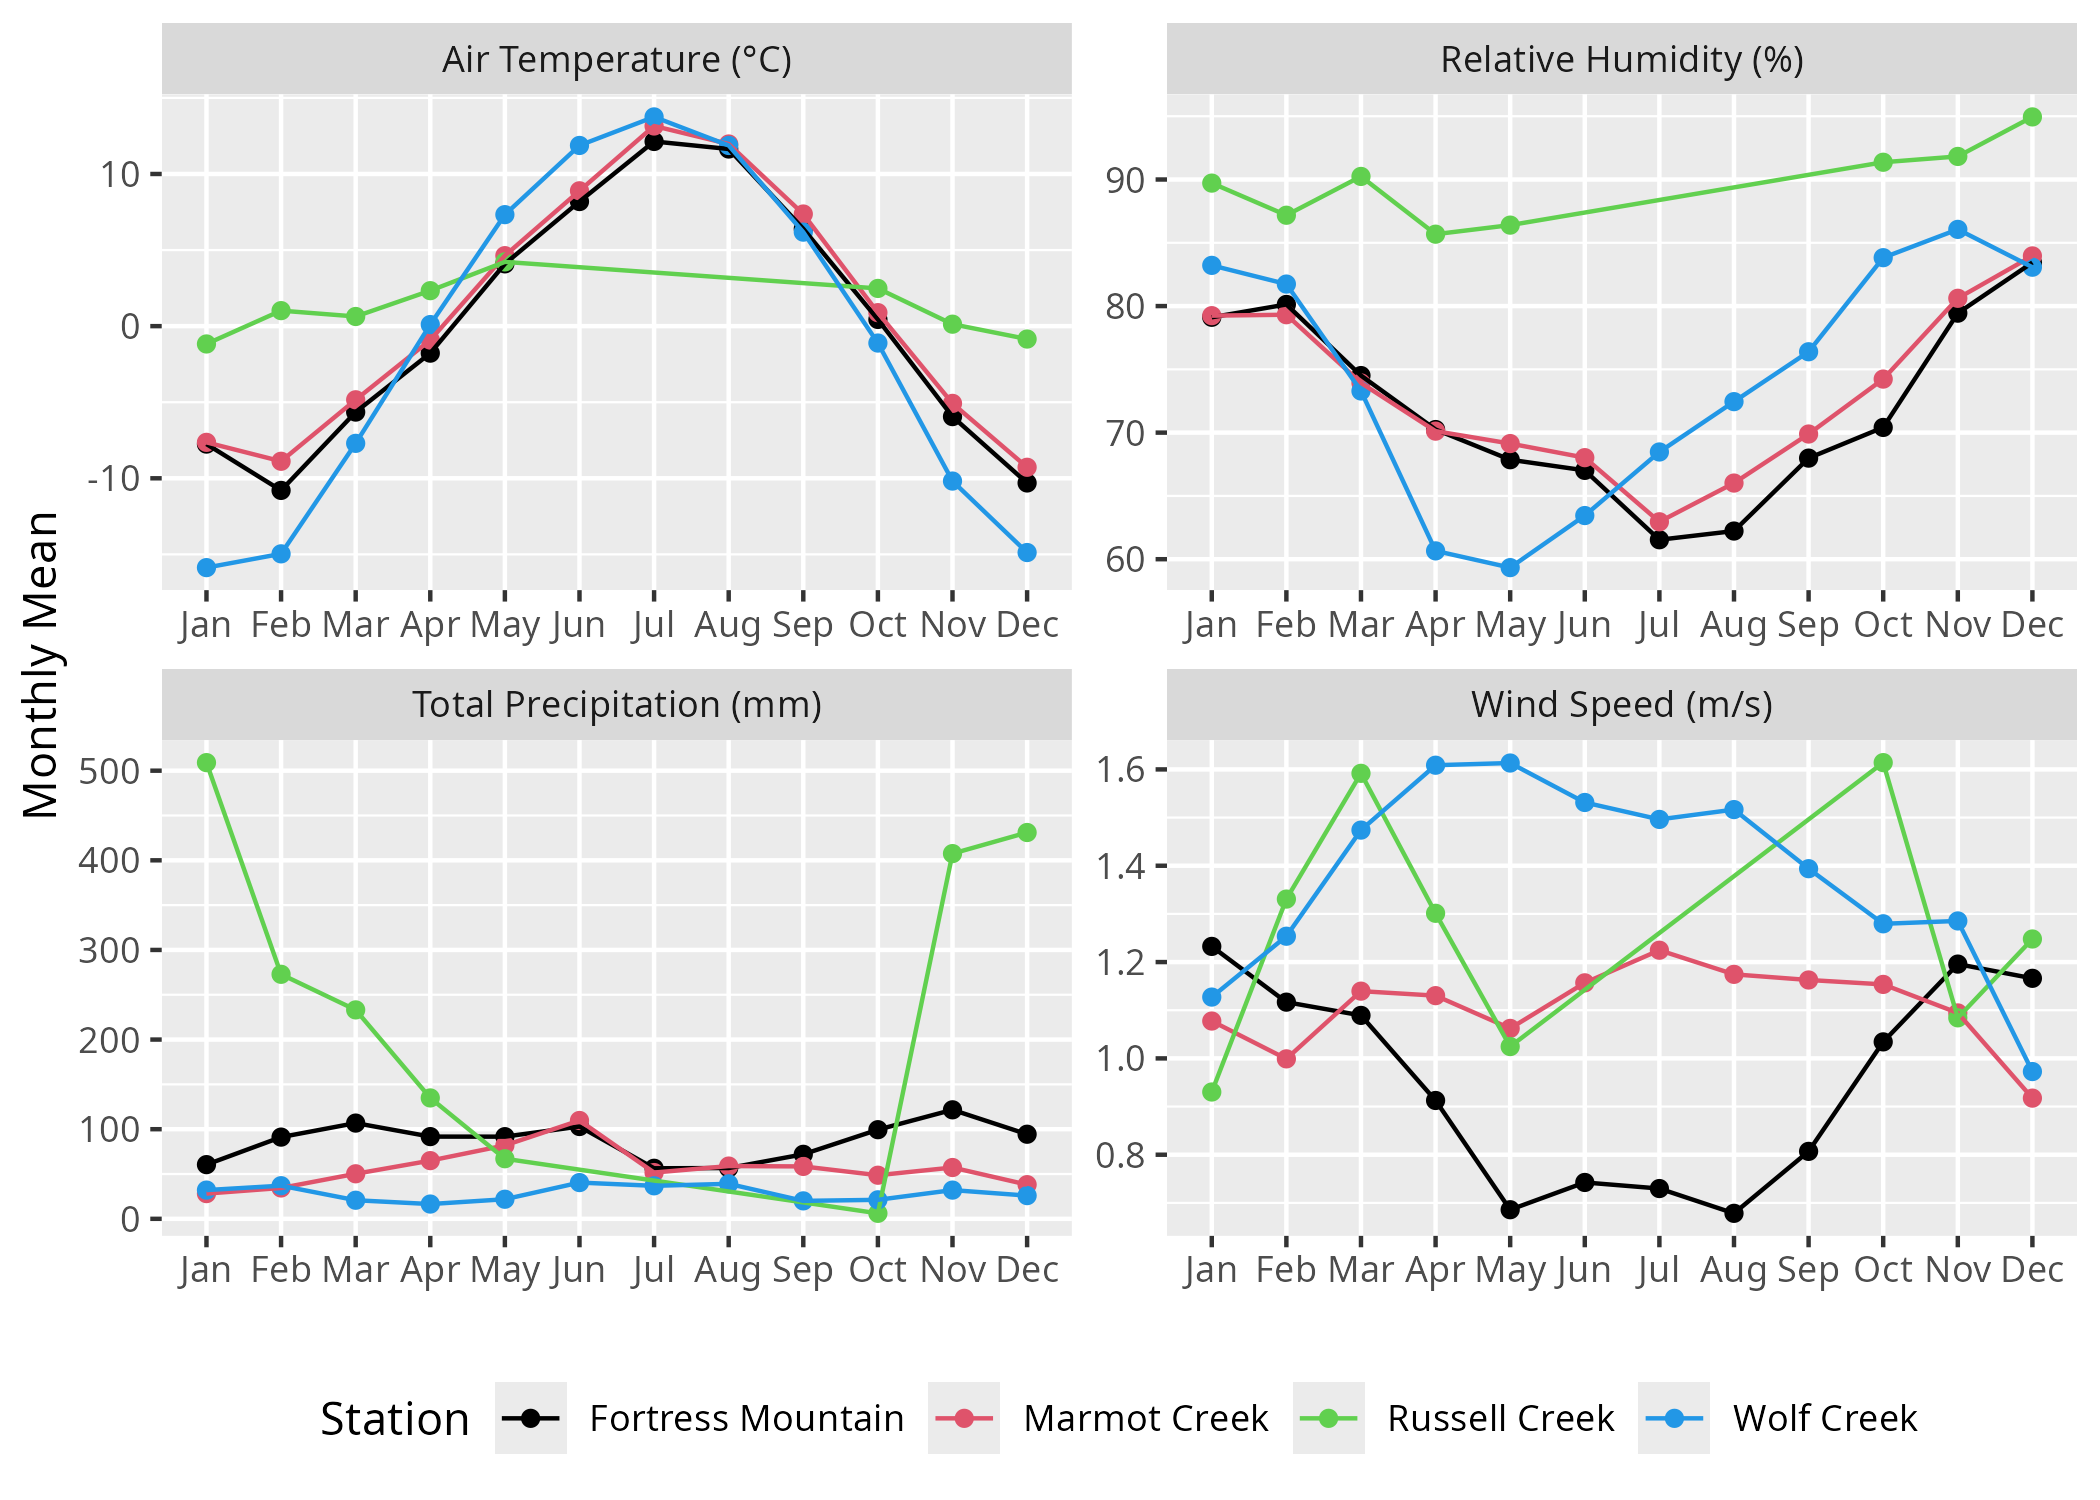
\includegraphics[keepaspectratio]{chapters/05-model-eval-paper/figs/figure2.png}}

}

\caption{\label{fig-met-normals}Graph showing mean monthly relative
humidity, air temperature, total precipitation, and wind speed over the
simulation period for each station. See Table~\ref{tbl-site-meta} for
the corresponding date ranges of each site. Observations were not
available during the snow free period for Russell Creek (Jun---Sept).}

\end{figure}%

\subsection{Simulation of Subcanopy
Snowpack}\label{simulation-of-subcanopy-snowpack}

The Cold Regions Hydrological Modelling Platform (CRHM) was implemented
to simulate SWE at each of the four forest plots. The CRHM platform is
described in detail in Pomeroy et al. (2022); and the up-to-date source
code is available at https://github.com/srlabUsask/crhmcode. Hourly
climate forcing data from station-based measurements of air temperature,
relative humidity, wind speed, total precipitation, and above canopy
incoming solar radiation were used to run the CRHM models. Incoming
solar radiation observations were not available for Wolf Creek and were
simulated following theoretical clear-sky radiation by Garnier \& Ohmura
(1970) and atmospheric transmittance by Annandale et al. (2002) and
Shook \& Pomeroy (2011).

Atmospheric precipitation was partitioned into snow and/or rain phases
following the psychometric energy balance approach of Harder \& Pomeroy
(2013) which accounts for the influence of temperature and humidity on
precipitation phase. The interaction of incoming precipitation with the
forest canopy was treated using two different approaches. An updated
approach following new relationships presented in Cebulski \& Pomeroy
(2025b) and Cebulski \& Pomeroy (2025c) (CP25) to represent the canopy
snow energy and mass balance were integrated within CRHM. This new
approach simulates initial interception of snow in the canopy as a
function of canopy density (Cebulski \& Pomeroy, 2025b) and subsequent
ablation of snow intercepted in the canopy by melt and dry-snow
unloading (Cebulski \& Pomeroy, 2025c), energy balance-based snowmelt
(Cebulski \& Pomeroy, 2025c), and energy balance-based sublimation
(Essery et al., 2003). A second approach (E10) which is based on
observations by Hedstrom \& Pomeroy (1998), Pomeroy et al. (1998b), and
Floyd (2012); and implemented as described in Ellis et al. (2010). E10
calculates initial interception of snow in the canopy as a function of
canopy density, antecedent snow load, and a species dependent storage
capacity following Hedstrom \& Pomeroy (1998). Ablation of snow
intercepted in the canopy is determined by dry snow unloading (function
of canopy snow load as in Hedstrom \& Pomeroy, 1998), unloading due to
melt (Ellis et al., 2010), canopy snowmelt drainage (threshold function
of ice-bulb temperature as in Ellis et al., 2010), and sublimation by an
analytical energy balance-based parameterisation (Pomeroy et al.,
1998b). See Cebulski \& Pomeroy (2025a) for a complete description of
the E10 parameterisation. While neither the E10 nor CP25 model was
calibrated for this study, their parameterisations were originally
developed using data from Marmot and Fortress, respectively.

A two-layer energy and mass balance snowmelt model (Snobal, Marks et
al., 1998) was used to calculate subcanopy snowpack processes. Net
shortwave radiation to the subcanopy snowpack was simulated by
calculating the transmittance of irradiance through the canopy, less the
amount reflected from the snow surface (Ellis et al., 2010; Pomeroy et
al., 2009). Incoming longwave radiation to subcanopy snow was simulated
by thermal emissions from the atmosphere and vegetation elements,
weighted by sky-view-factor (Ellis et al., 2010; Pomeroy et al., 2009).
Sensible and latent heat fluxes to the subcanopy snowpack were
determined using an approach adopted from Brutsaert (1982) and Marks \&
Dozier (1992) and is described in the CRHM source code. Only two water
years were simulated at Russell due to limited model forcing and
validation data.

\subsection{Model Evaluation}\label{model-evaluation}

Simulated subcanopy SWE by the two models (E10 and CP25) was evaluated
using snow survey observations collected from transects at the four
forest plots. The performance of the two models was evaluated based on
the differences in simulated (\(S_i\)) and observed (\(O_i\)) values of
SWE using mean bias (MB) and root mean squared error (RMSE) as:

\begin{equation}\phantomsection\label{eq-mb}{
\text{MB} = \frac{1}{n} \sum^n_{i=1}(S_i-O_i)
}\end{equation}

and

\begin{equation}\phantomsection\label{eq-rmse}{
\text{RMSE} = \sqrt{\frac{\sum^n_{i=1}(S_i-O_i)^2}{n}}
}\end{equation}

Values for \(S_i\) were selected for each site from the E10 and CP25
CRHM simulated SWE state for the timestamp that matched each of the snow
survey observations (\(O_i\)). The MB and RMSE statistics represent the
model performance over all simulation years for each site.

\section{Results}\label{results-2}

\subsection{Snowpack Observations}\label{snowpack-observations}

Amongst the sites and years included in the study, accumulation of
snowfall below the canopy was less than cumulative snowfall, as observed
in open clearings adjacent to each forest transect
(Figure~\ref{fig-sf-subcpy-swe}). At peak seasonal subcanopy SWE,
Fortress had the highest fraction of seasonal snowfall stored in the
subcanopy snowpack at 0.6, followed by Marmot and Wolf Creek which both
had similar fractions at 0.4, and Russell had the smallest fraction at
0.3 when averaged over all years. Variations in the prevalence of canopy
snow unloading, melt/drip, and sublimation contributed to the observed
differences in subcanopy snow accumulation relative to the open
clearings at each site. At the temperate-maritime Russell site
mid-winter melt events also contributed to these observed differences.
Following validation of the new CP25 model in representing subcanopy
SWE, a diagnosis on the contribution of each canopy snow processes in
influencing subcanopy snowfall accumulation will be conducted in
Section~\ref{sec-sf-partition} for each site.

\begin{figure}

\centering{

\pandocbounded{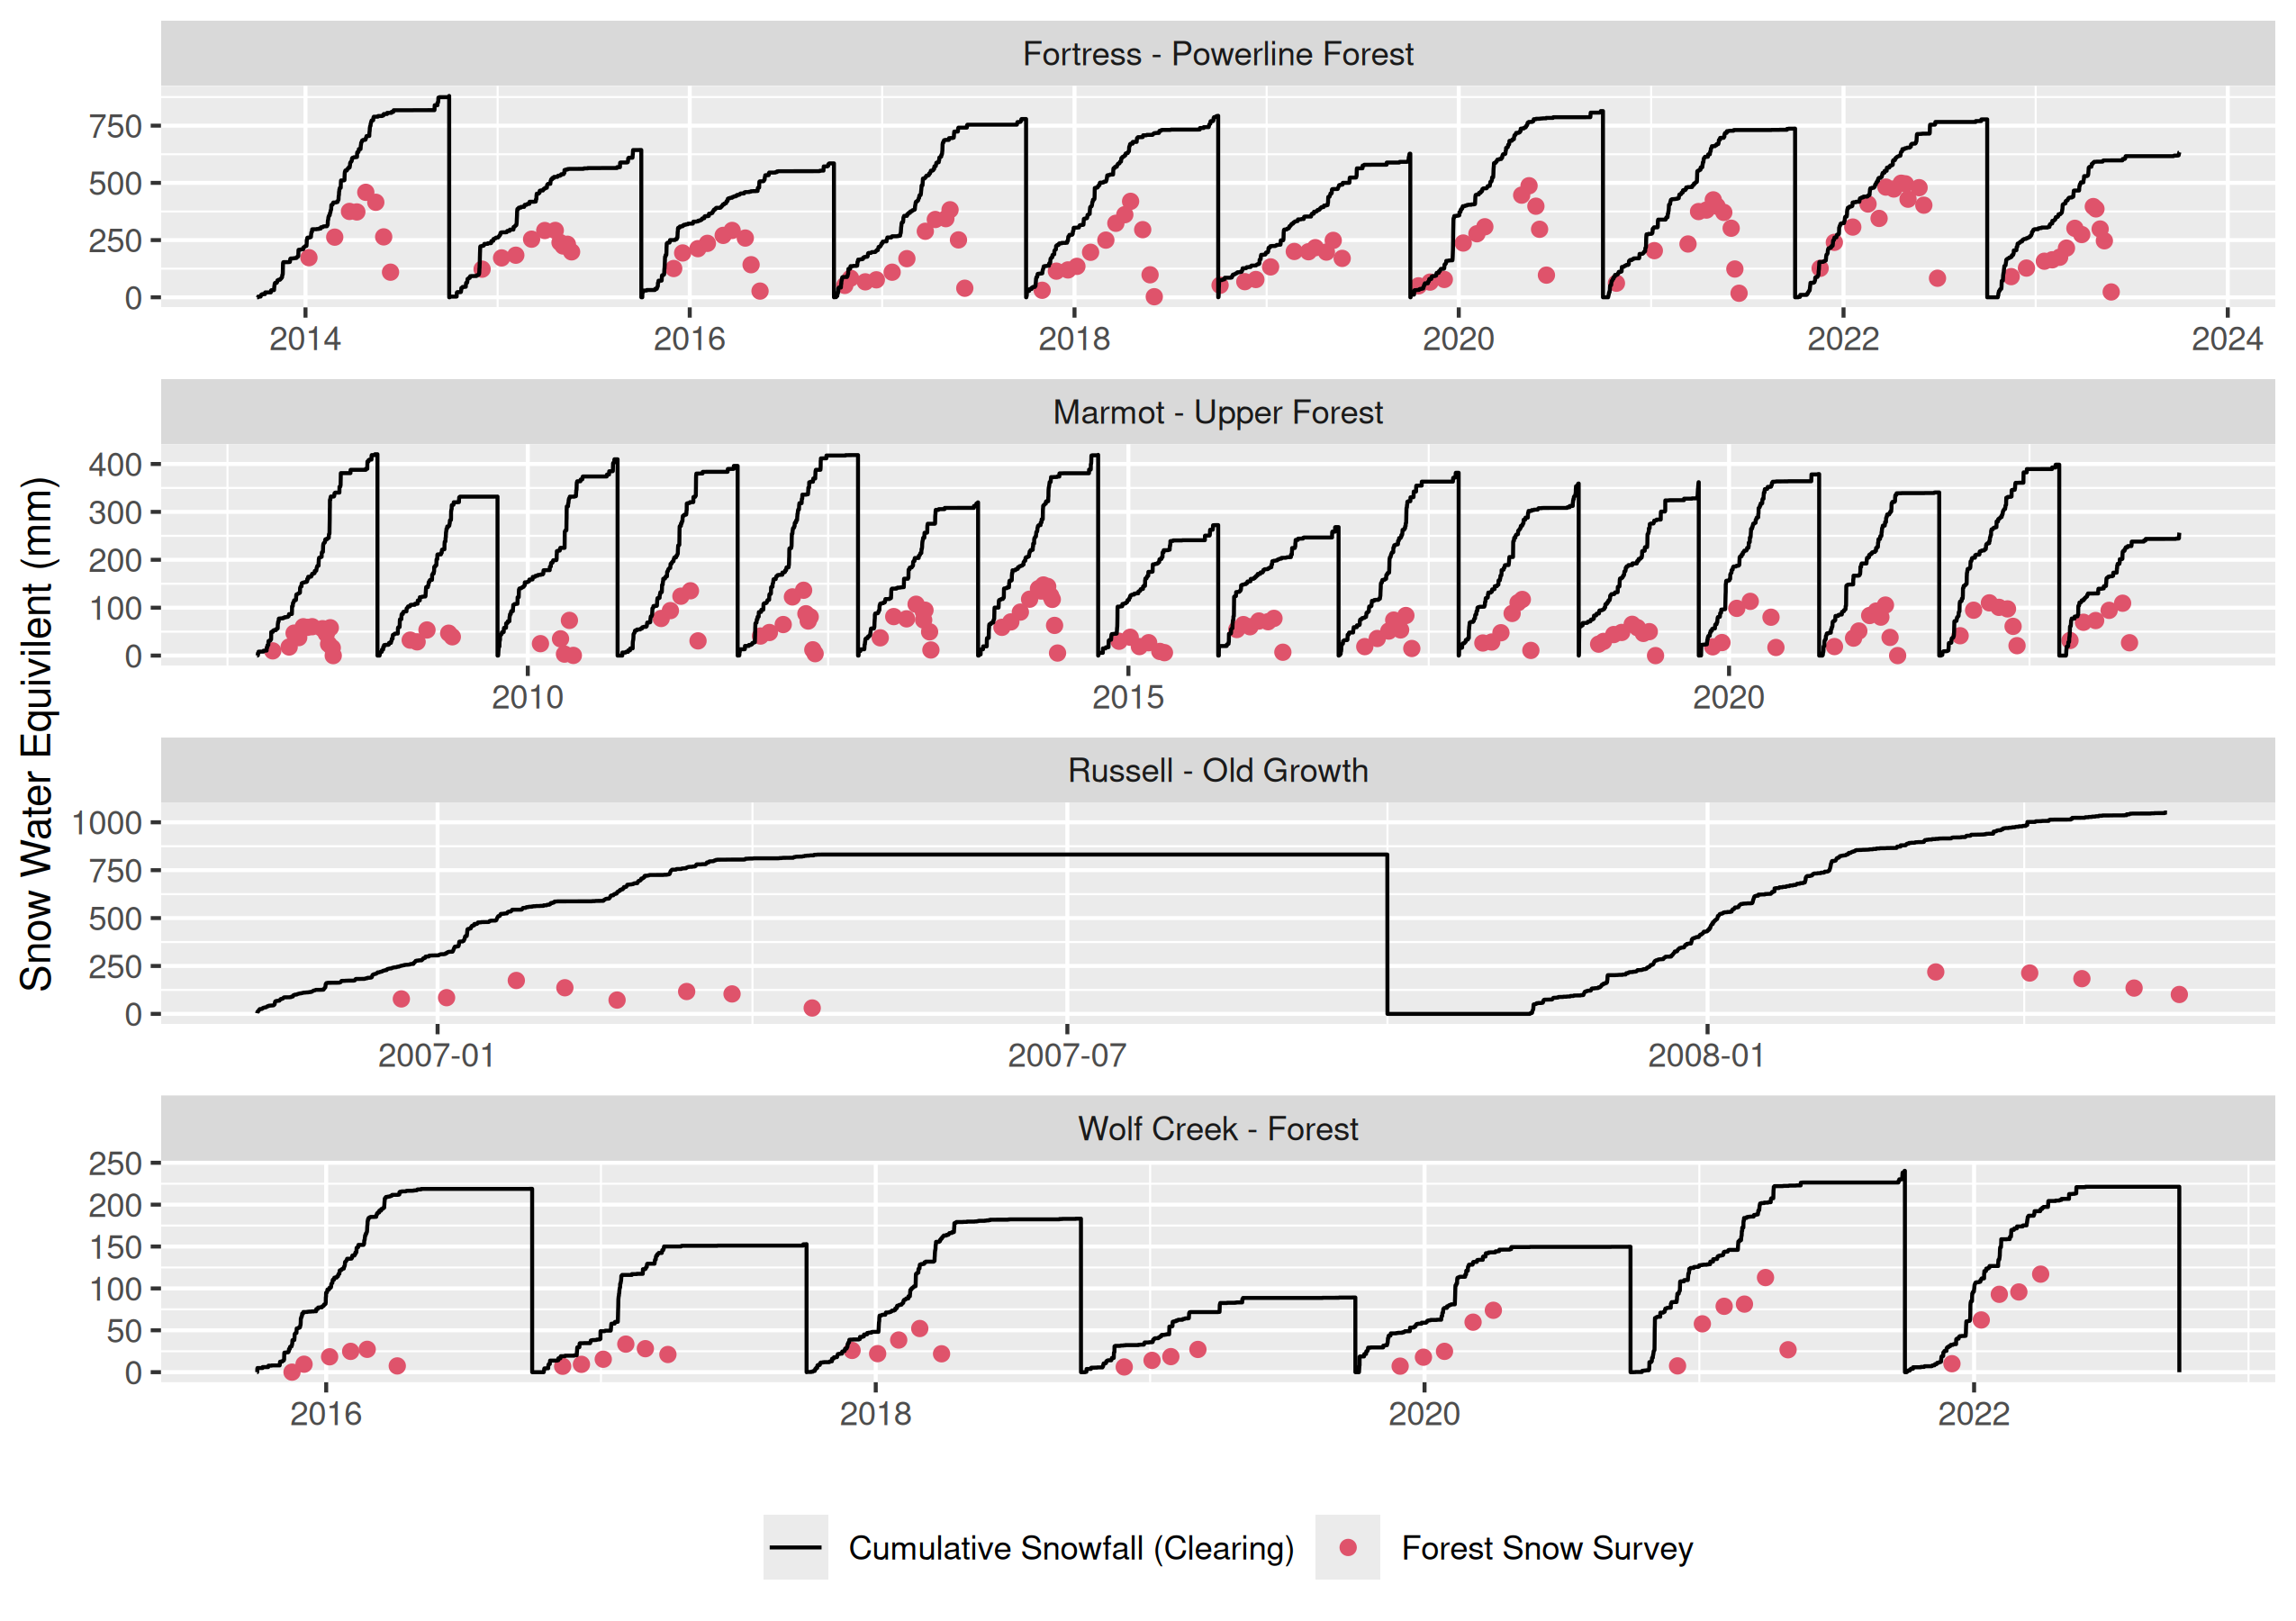
\includegraphics[keepaspectratio]{chapters/05-model-eval-paper/figs/figure3_a.png}}

}

\caption{\label{fig-sf-subcpy-swe}Time series showing seasonal
cumulative snowfall (black lines) and subcanopy snow water equivalent
from in situ snow surveys (red dots). Note: snowfall was determined from
observed total precipitation for each site using the snowfall fraction
simulated in CRHM following Harder \& Pomeroy (2013).}

\end{figure}%

Observed subcanopy SWE varied from a seasonal mean of 14.6 to 366.8 kg
m\textsuperscript{-2} (Figure~\ref{fig-swe-ann-mean}) and seasonal peak
SWE varied from 27.1 to 498.4 kg m\textsuperscript{-2}
(Figure~\ref{fig-swe-ann-peak}) across all sites and years. The CP25
model tended to underestimate both mean and peak SWE at these three
colder sites while E10 overestimated SWE at all four sites.

\begin{figure}

\centering{

\pandocbounded{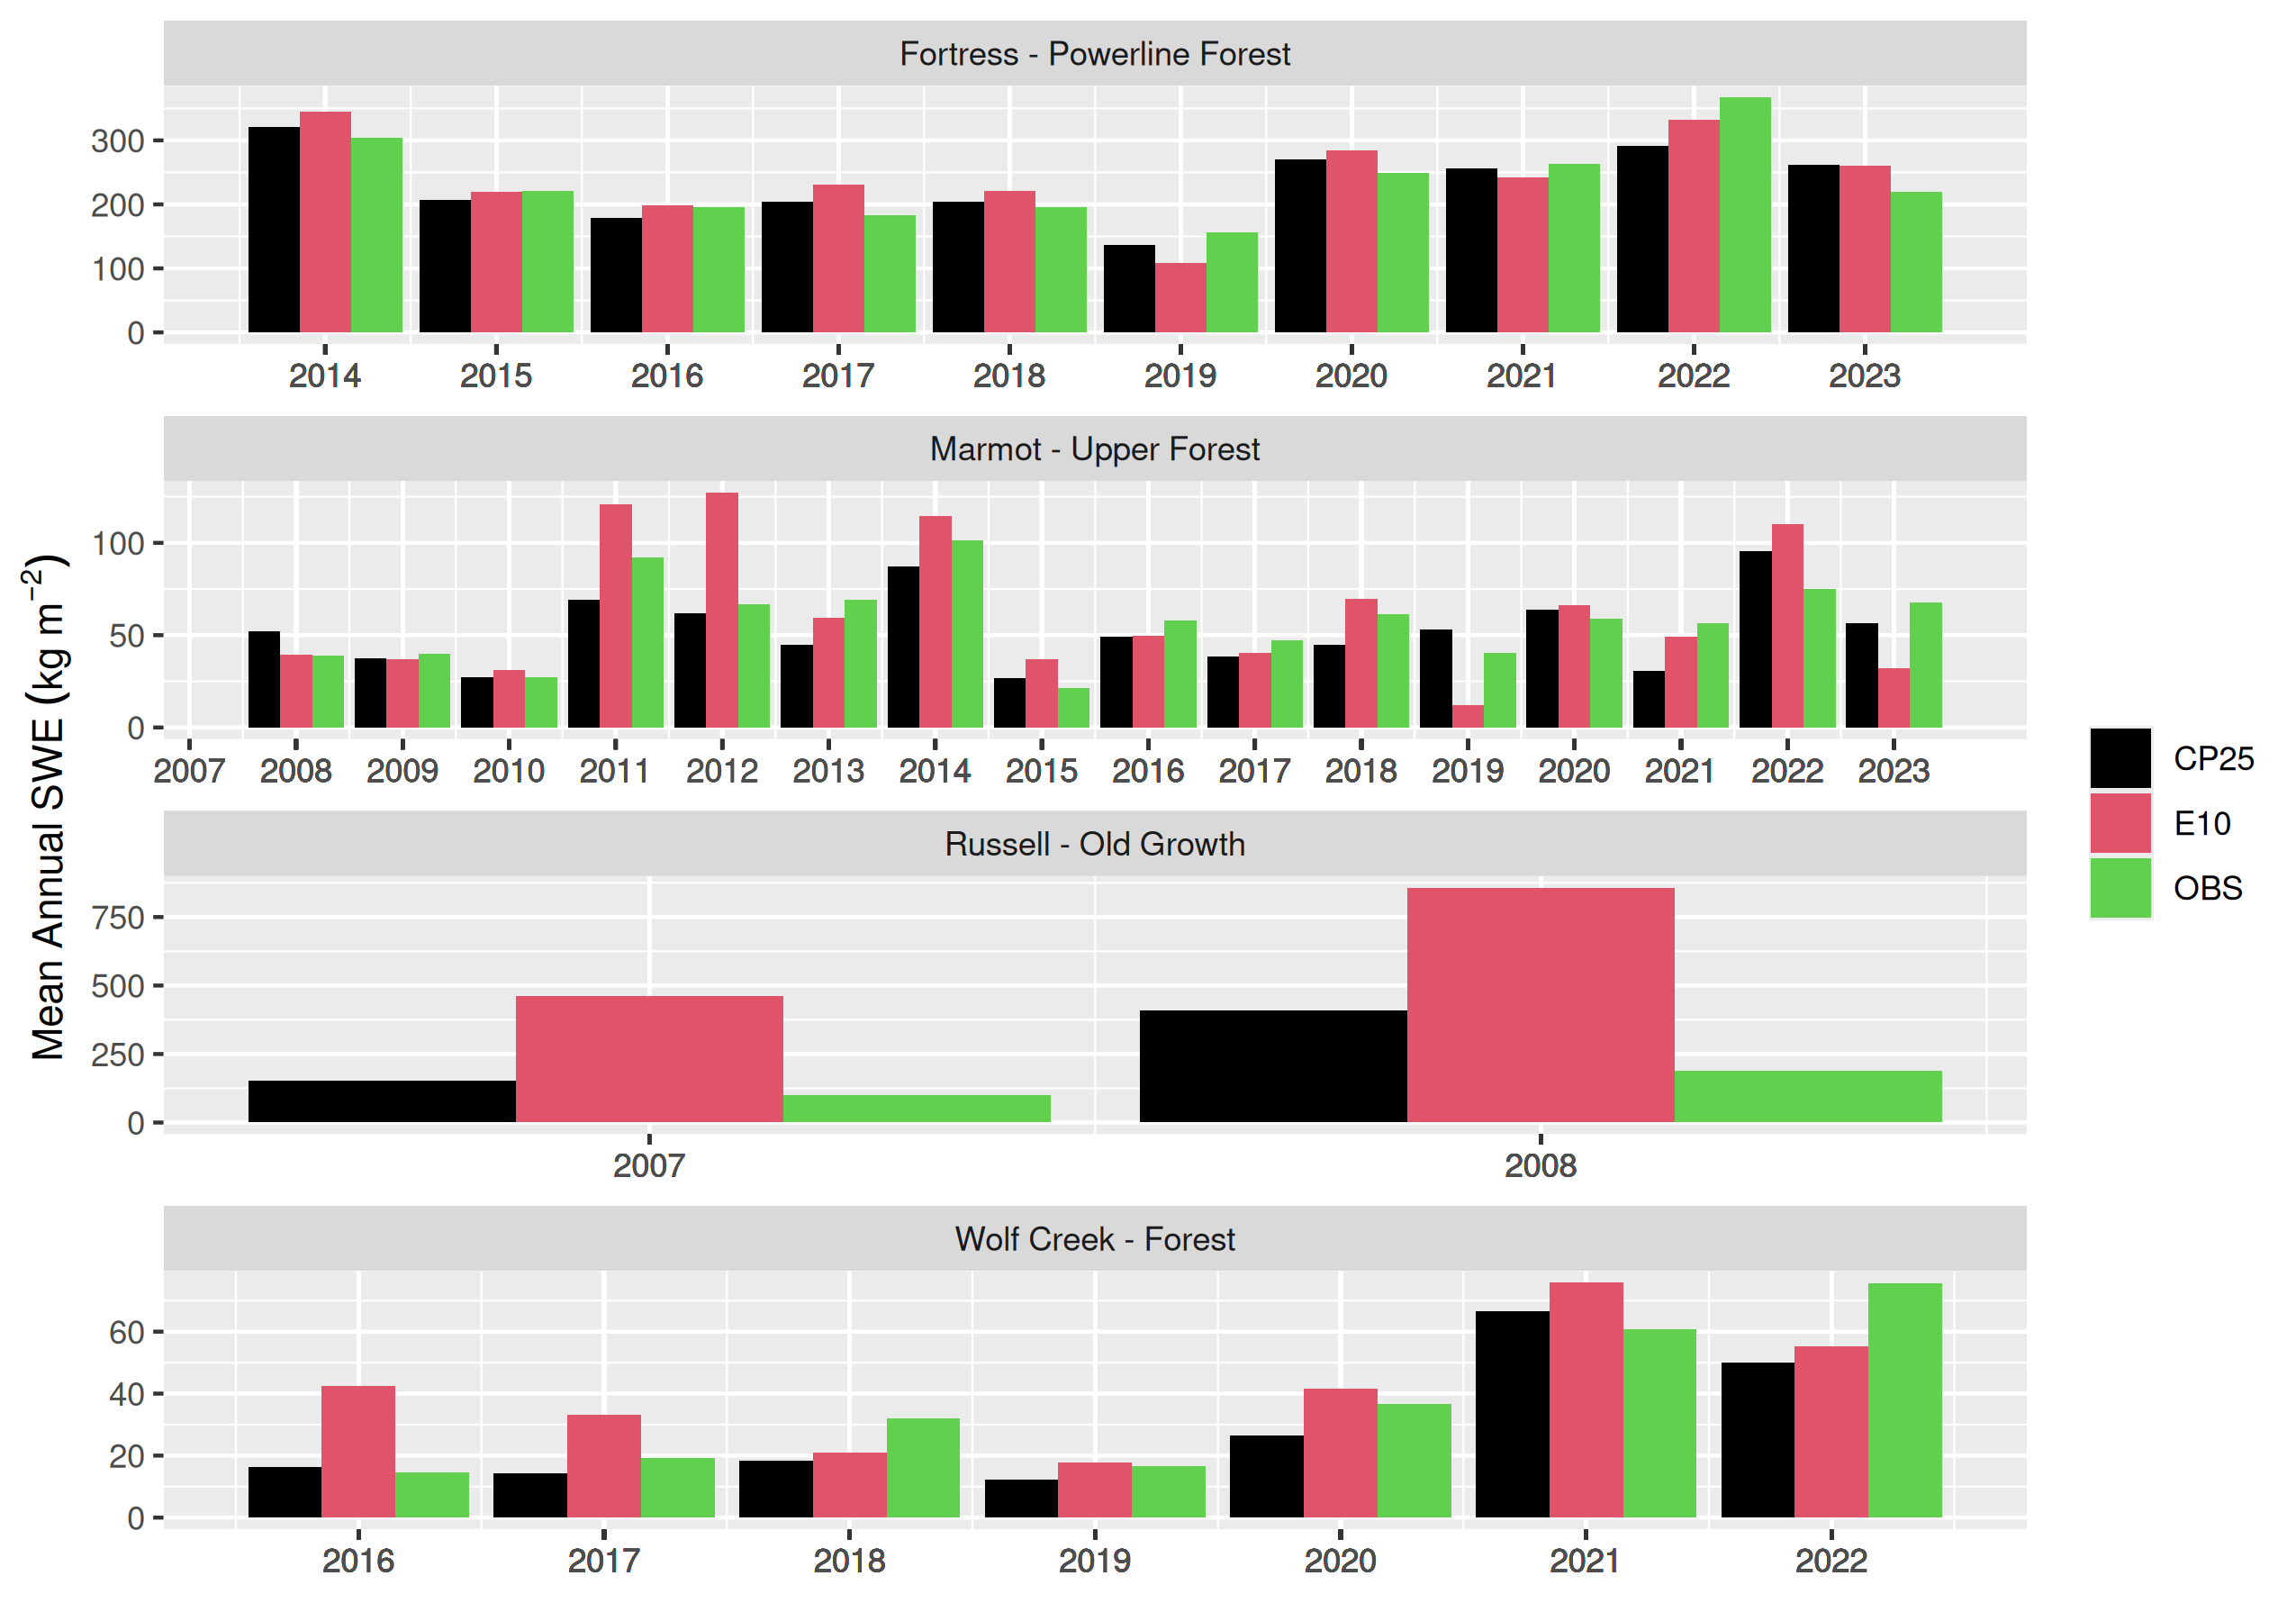
\includegraphics[keepaspectratio]{chapters/05-model-eval-paper/figs/figure3.png}}

}

\caption{\label{fig-swe-ann-mean}Bar chart comparing mean water year
snow water equivalent between snow survey observations (OBS) and the two
models (CP25 and E10).}

\end{figure}%

\begin{figure}

\centering{

\pandocbounded{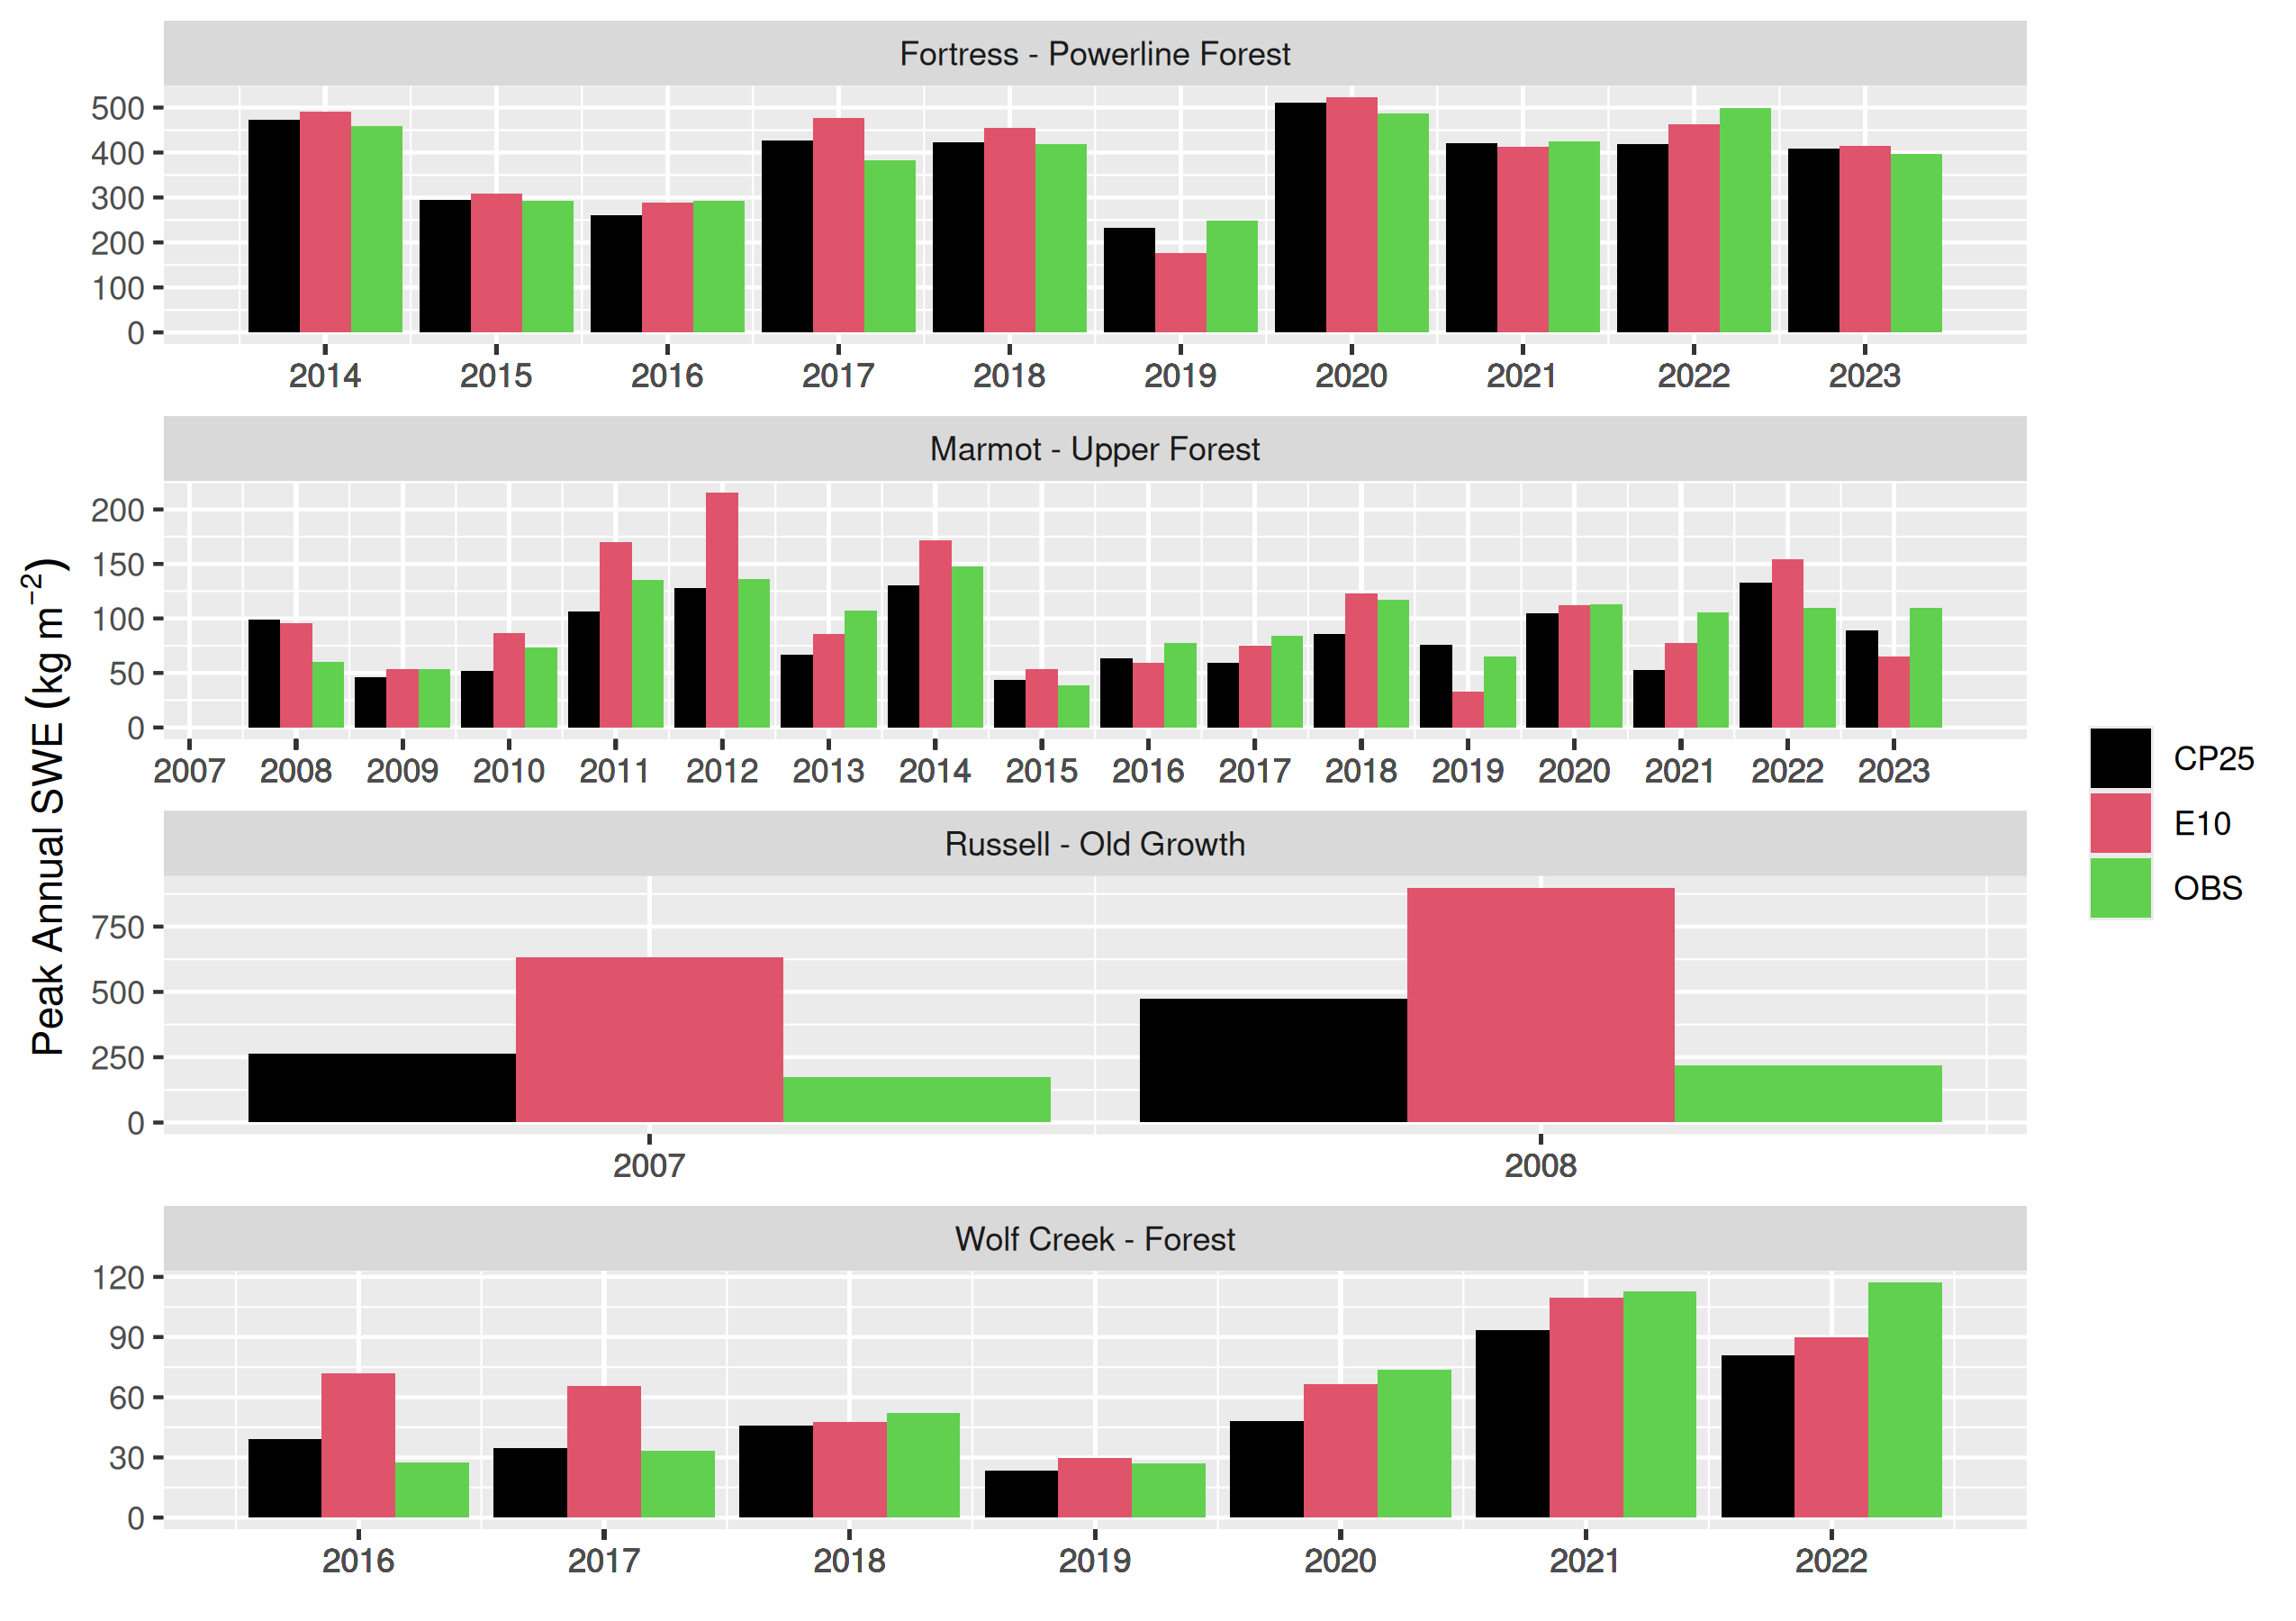
\includegraphics[keepaspectratio]{chapters/05-model-eval-paper/figs/figure4.png}}

}

\caption{\label{fig-swe-ann-peak}Bar chart comparing peak water year
snow water equivalent between snow survey observations (OBS) and the two
models (CP25 and E10).}

\end{figure}%

\subsection{Evaluation of Snowpack
Models}\label{evaluation-of-snowpack-models}

Over all years and sites, the CP25 model had a lower mean bias of -0.63
kg m\textsuperscript{-2} compared to E10's mean bias of -26.23 kg
m\textsuperscript{-2} in representing the individual subcanopy SWE
measurements shown in Figure~\ref{fig-swe-ts}. Across the three colder
climate sites (i.e., Fortress, Marmot, and Wolf Creek) CP25
underestimated SWE (MB = 3.38 kg m\textsuperscript{-2}) and E10
overestimated SWE (MB = -11.5 kg m\textsuperscript{-2}). CP25 had its
smallest mean bias at Fortress of 2.53 kg m\textsuperscript{-2}---where
the canopy snow energy and mass balance parameterisations were
developed---followed by Marmot, Wolf Creek, and Russell. E10 had its
lowest mean bias at Marmot---where this canopy snow model had previously
been tested and developed---followed by Wolf Creek, Fortress, and
Russell (Table~\ref{tbl-swe-mb}). Both the CP25 and E10 models had
relatively similar performance at Marmot and Wolf Creek based on their
mean biases which had absolute values which differed by less than 1 kg
m\textsuperscript{-2} (Table~\ref{tbl-swe-mb}). Although E10 had a
marginally reduced mean bias at Wolf Creek of -5.81 kg
m\textsuperscript{-2} compared to 6.72 kg m\textsuperscript{-2} for CP25
the RMSE across all sites was lower for CP25 (Table~\ref{tbl-swe-mb}).
The lower RMSE for CP25 compared to E10 is also reflected in CP25's
closer estimates to mean and peak seasonal SWE across all water years
across all four sites compared to E10 (Figure~\ref{fig-swe-ann-mean};
Figure~\ref{fig-swe-ann-peak}). Three years contributed to the higher
RMSE at Marmot where E10 simulated SWE was greatly overestimated based
on a mean and peak value by over 50 kg m\textsuperscript{-2} (nearly
100\% of observed SWE) for the water years 2011 and 2012
(Figure~\ref{fig-swe-ann-mean}; Figure~\ref{fig-swe-ann-peak}). In
contrast, E10 had a very large underestimation in subcanopy SWE at
Marmot for the water year 2019. At Wolf Creek, E10 also had deviations
of \textasciitilde30 kg m\textsuperscript{-2} (\textasciitilde100\%
greater than observed SWE) from observed mean and peak seasonal SWE for
2016 and 2017. Both models had their worst overall performance for the
temperate-maritime Russell site; however, CP25 did show a substantial
improvement compared to the E10 model with mean biases of -108.87 kg
m\textsuperscript{-2} and -465.37 kg m\textsuperscript{-2} respectively.
Although the intent of this evaluation is to assess the performance of
each model in simulating subcanopy SWE, uncertainties in model forcing
and physical parameters (i.e., canopy coverage, LAI) may also contribute
to systematic biases in the evaluation. Some of the increased model
error at Russell during the 2008 water year may reflect the use of total
precipitation data from a nearby highway station rather than on-site
measurements.

\begin{longtable}[]{@{}llrr@{}}

\caption{\label{tbl-swe-mb}Mean bias (MB) and and root mean squared
error (RMSE) determined from time-series simulations of snow water
equivalent for the two canopy snow models at each of the four sites.}

\tabularnewline

\toprule\noalign{}
Model & Station & MB & RMSE \\
\midrule\noalign{}
\endhead
\bottomrule\noalign{}
\endlastfoot
CP25 & Fortress - Powerline Forest & 2.53 & 46.10 \\
CP25 & Marmot - Upper Forest & 4.88 & 20.92 \\
CP25 & Russell - Old Growth & -108.87 & 141.79 \\
CP25 & Wolf Creek - Forest & 6.72 & 17.62 \\
CP25 & All Station Mean & -0.63 & 43.70 \\
E10 & Fortress - Powerline Forest & -8.94 & 53.84 \\
E10 & Marmot - Upper Forest & -5.02 & 30.62 \\
E10 & Russell - Old Growth & -465.37 & 499.99 \\
E10 & Wolf Creek - Forest & -5.81 & 21.93 \\
E10 & All Station Mean & -26.23 & 110.61 \\

\end{longtable}

Seasonal subcanopy SWE accumulation and ablation was generally well
represented by both models at Fortress, Marmot, and Wolf Creek
(Figure~\ref{fig-swe-ts}). However, E10 failed to simulate the timing of
SWE accumulation and ablation well for 2011, 2012, and 2019 at Marmot.
The largest deviation in simulated seasonal SWE occurred at Russell for
E10 where subcanopy snow accumulation was simulated at a much higher
rate compared to the observed and CP25 over the two years that were
simulated. At Wolf Creek CP25 had a delay in simulating the initial
accumulation of subcanopy SWE for water years 2017, 2018, and 2019. The
lower snowfall rate at Wolf Creek and higher interception rate for CP25
compared to E10 led to throughfall and unloading rates that were smaller
than the snowpack initiation threshold employed in Snobal, which Snobal
then melts SWE accumulations below this threshold completely. In
contrast, E10 intercepted less snow and had higher unloading rates than
CP25 leading to higher initial accumulation for these three years at
Wolf Creek.

\begin{figure}

\centering{

\pandocbounded{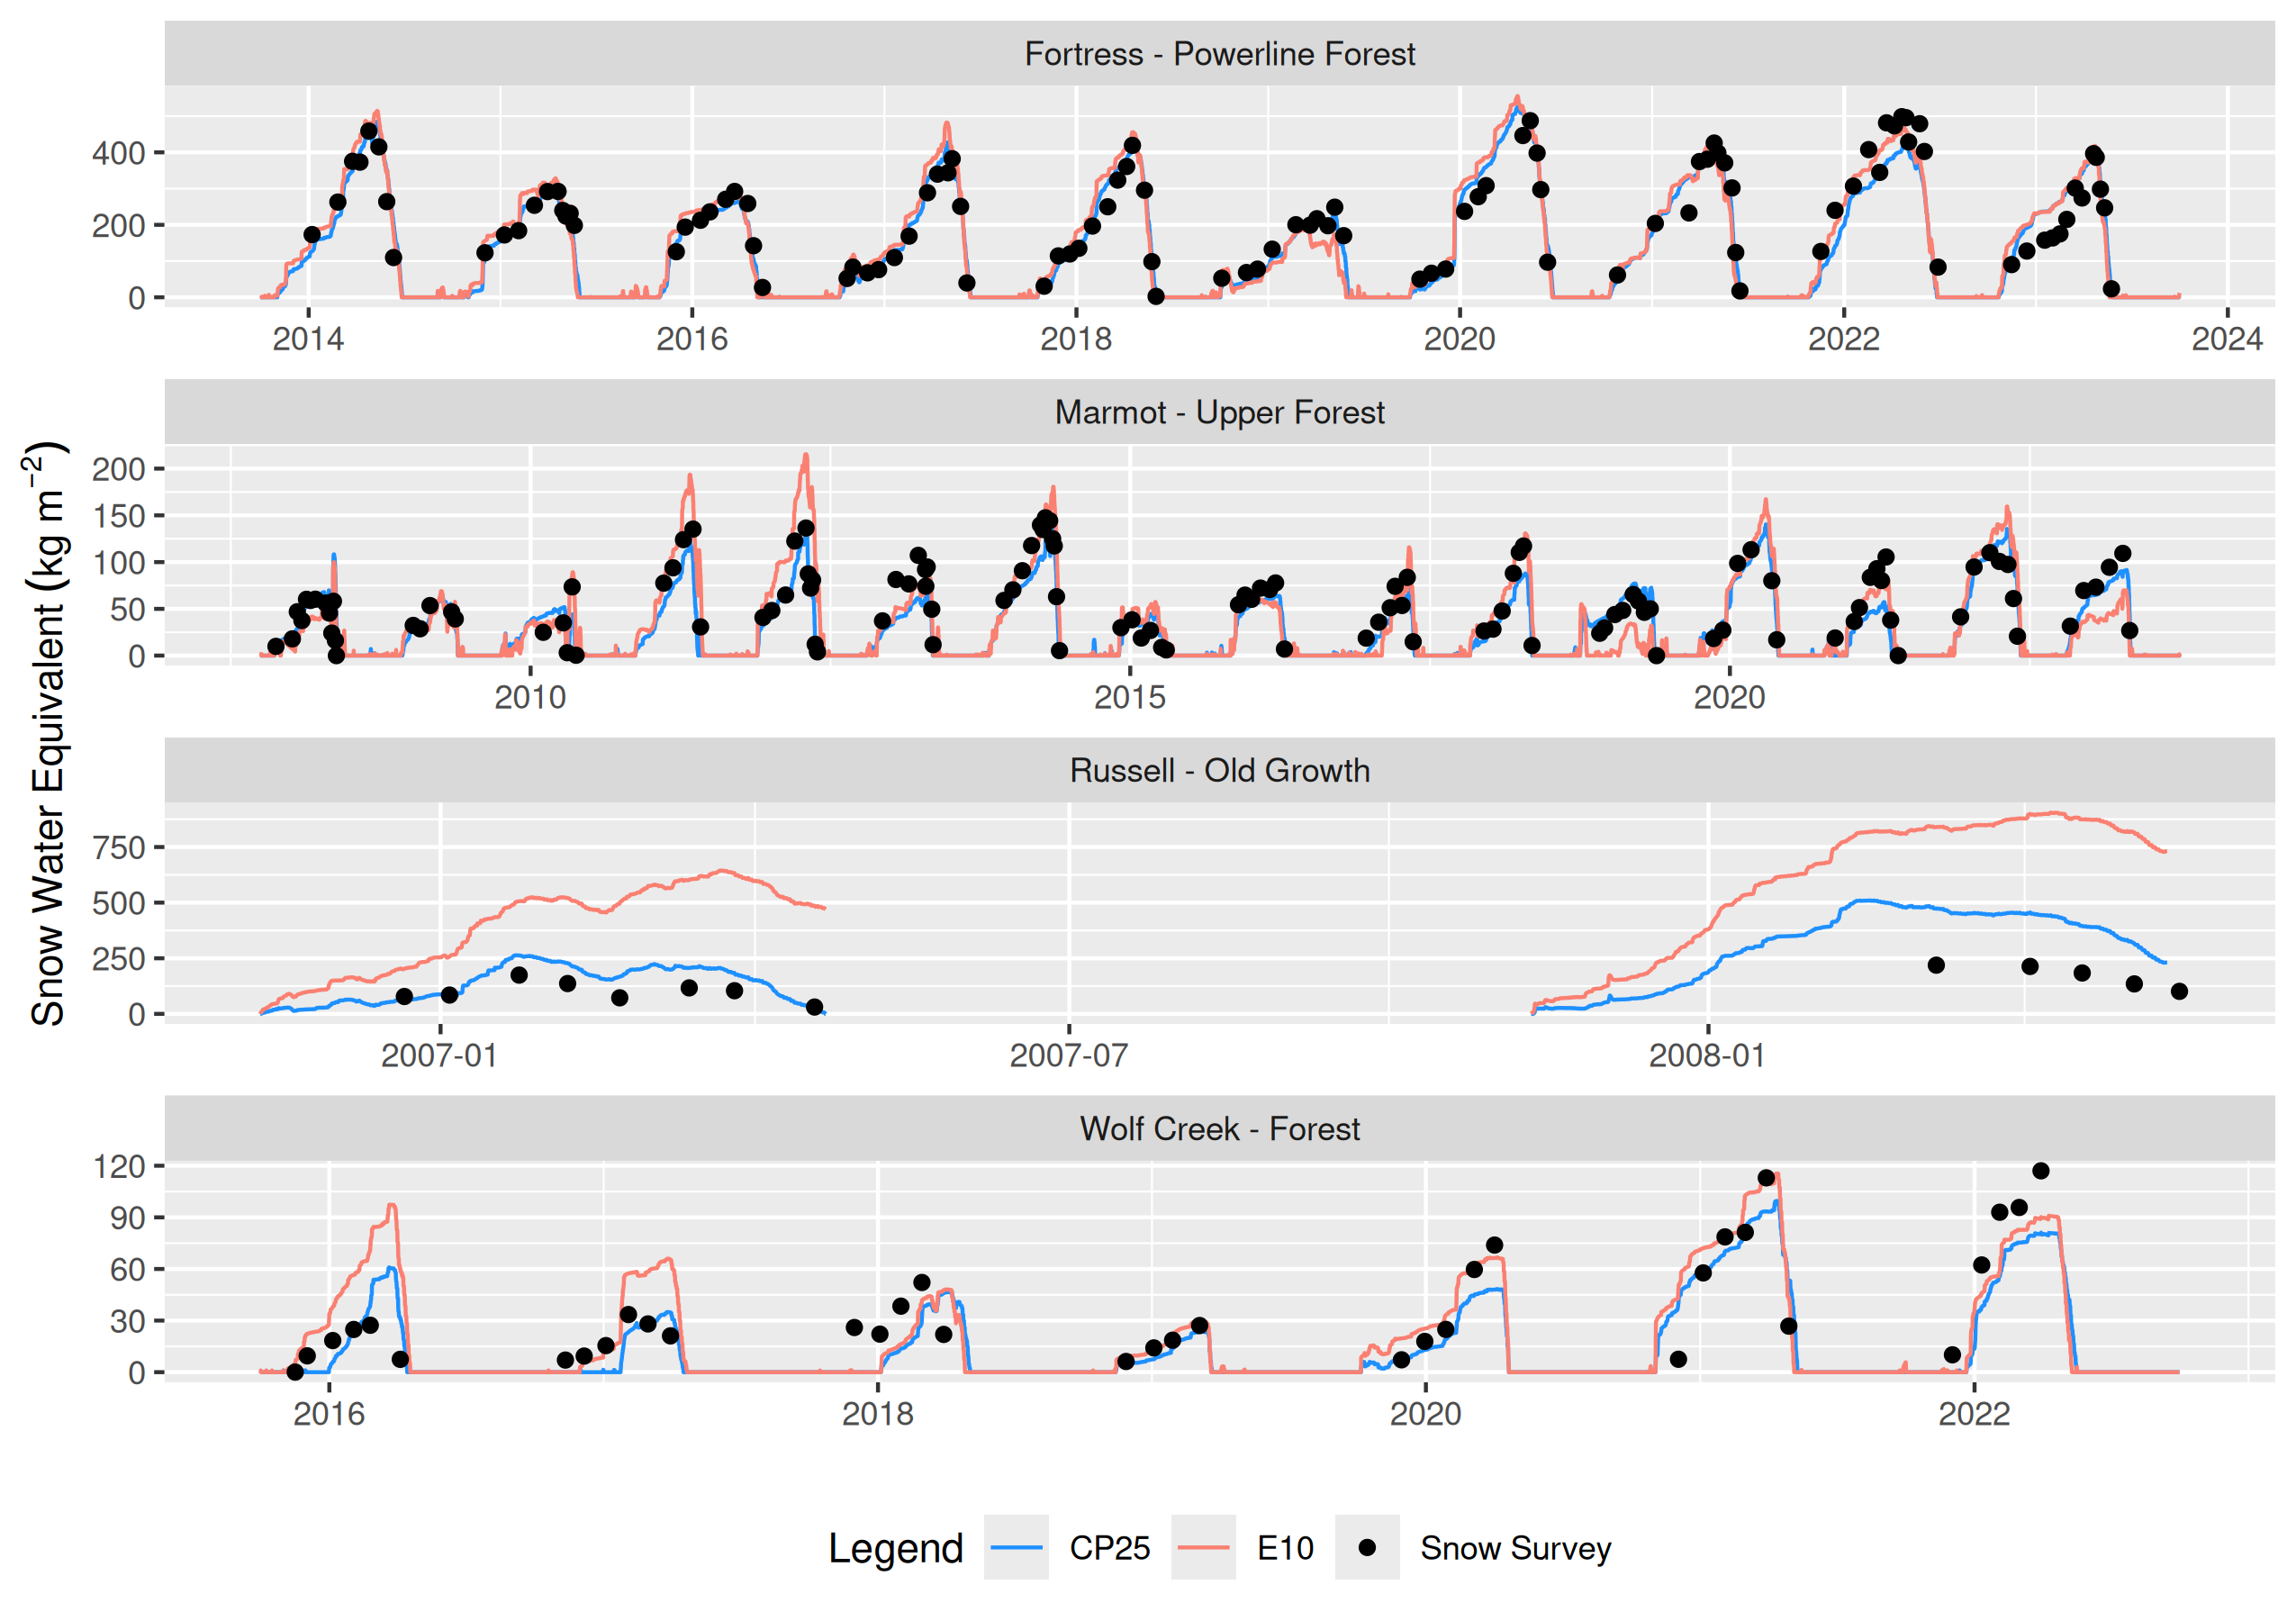
\includegraphics[keepaspectratio]{chapters/05-model-eval-paper/figs/figure5.png}}

}

\caption{\label{fig-swe-ts}Timeseries of observed and simulated (CP25
and E10) forest snow water equivalent at each station.}

\end{figure}%

\subsection{Snowfall Partitioning}\label{sec-sf-partition}

A greater fraction of annual snowfall was sublimated by CP25 compared to
E10 for all four sites across all years (Figure~\ref{fig-frac-subl}).
Lower interception efficiency combined with higher average rates of
unloading for the E10 model led to more snowfall being partitioned
towards the ground compared to the CP25 model
(Figure~\ref{fig-frac-unld}) leading to reduced sublimation of canopy
snow and thus overprediction of subcanopy SWE accumulation
(Table~\ref{tbl-swe-mb}). The underprediction of subcanopy SWE by the
CP25 model at Fortress, Marmot, and Wolf Creek (Table~\ref{tbl-swe-mb})
may have been due to an overestimate of sublimation and/or canopy
snowmelt rates leading to less snowfall being partitioned to the ground
as solid snow. The difference in the annual fraction of snowfall that
was sublimated between the CP25 and E10 models was most prevalent at
Marmot (Figure~\ref{fig-frac-subl}). Factors that may contribute to this
large deviation include the lower unloading rates observed for CP25 at
this site (Figure~\ref{fig-frac-unld}) compared to E10 resulting from
the lower wind speed and air temperatures at this site
(Figure~\ref{fig-met-normals}), reducing the unloading and canopy
snowmelt rates thus increasing the amount of canopy snow subject to
sublimation for CP25. For E10, the April---June monthly air temperature
normals at Marmot---months when this site receives most of its snowfall
(Figure~\ref{fig-met-normals})---are also largely within the E10
ice-bulb temperature unloading range (-3°C to 6°C) which are ideal
conditions for initiating unloading due to warming for the E10 model.
Relatively similar fractions of annual snowfall was sublimated by the
two models at Fortress and Wolf Creek (Figure~\ref{fig-frac-subl}) due
to the similar sublimation parameterisation used by the two models
combined with the similar fraction of snow partitioned towards the
ground (Figure~\ref{fig-frac-unld}). Although CP25 had higher drip/melt
rates than E10, increased throughfall by E10 coupled with the constant
unloading rate as a function of snow load likely made up for E10's lower
melt/drip rate (Figure~\ref{fig-frac-drip}). Process observations of
unloading, melt, and sublimation were not available and thus the
simulations of snowfall partitioning could not be directly evaluated.

\begin{figure}

\centering{

\pandocbounded{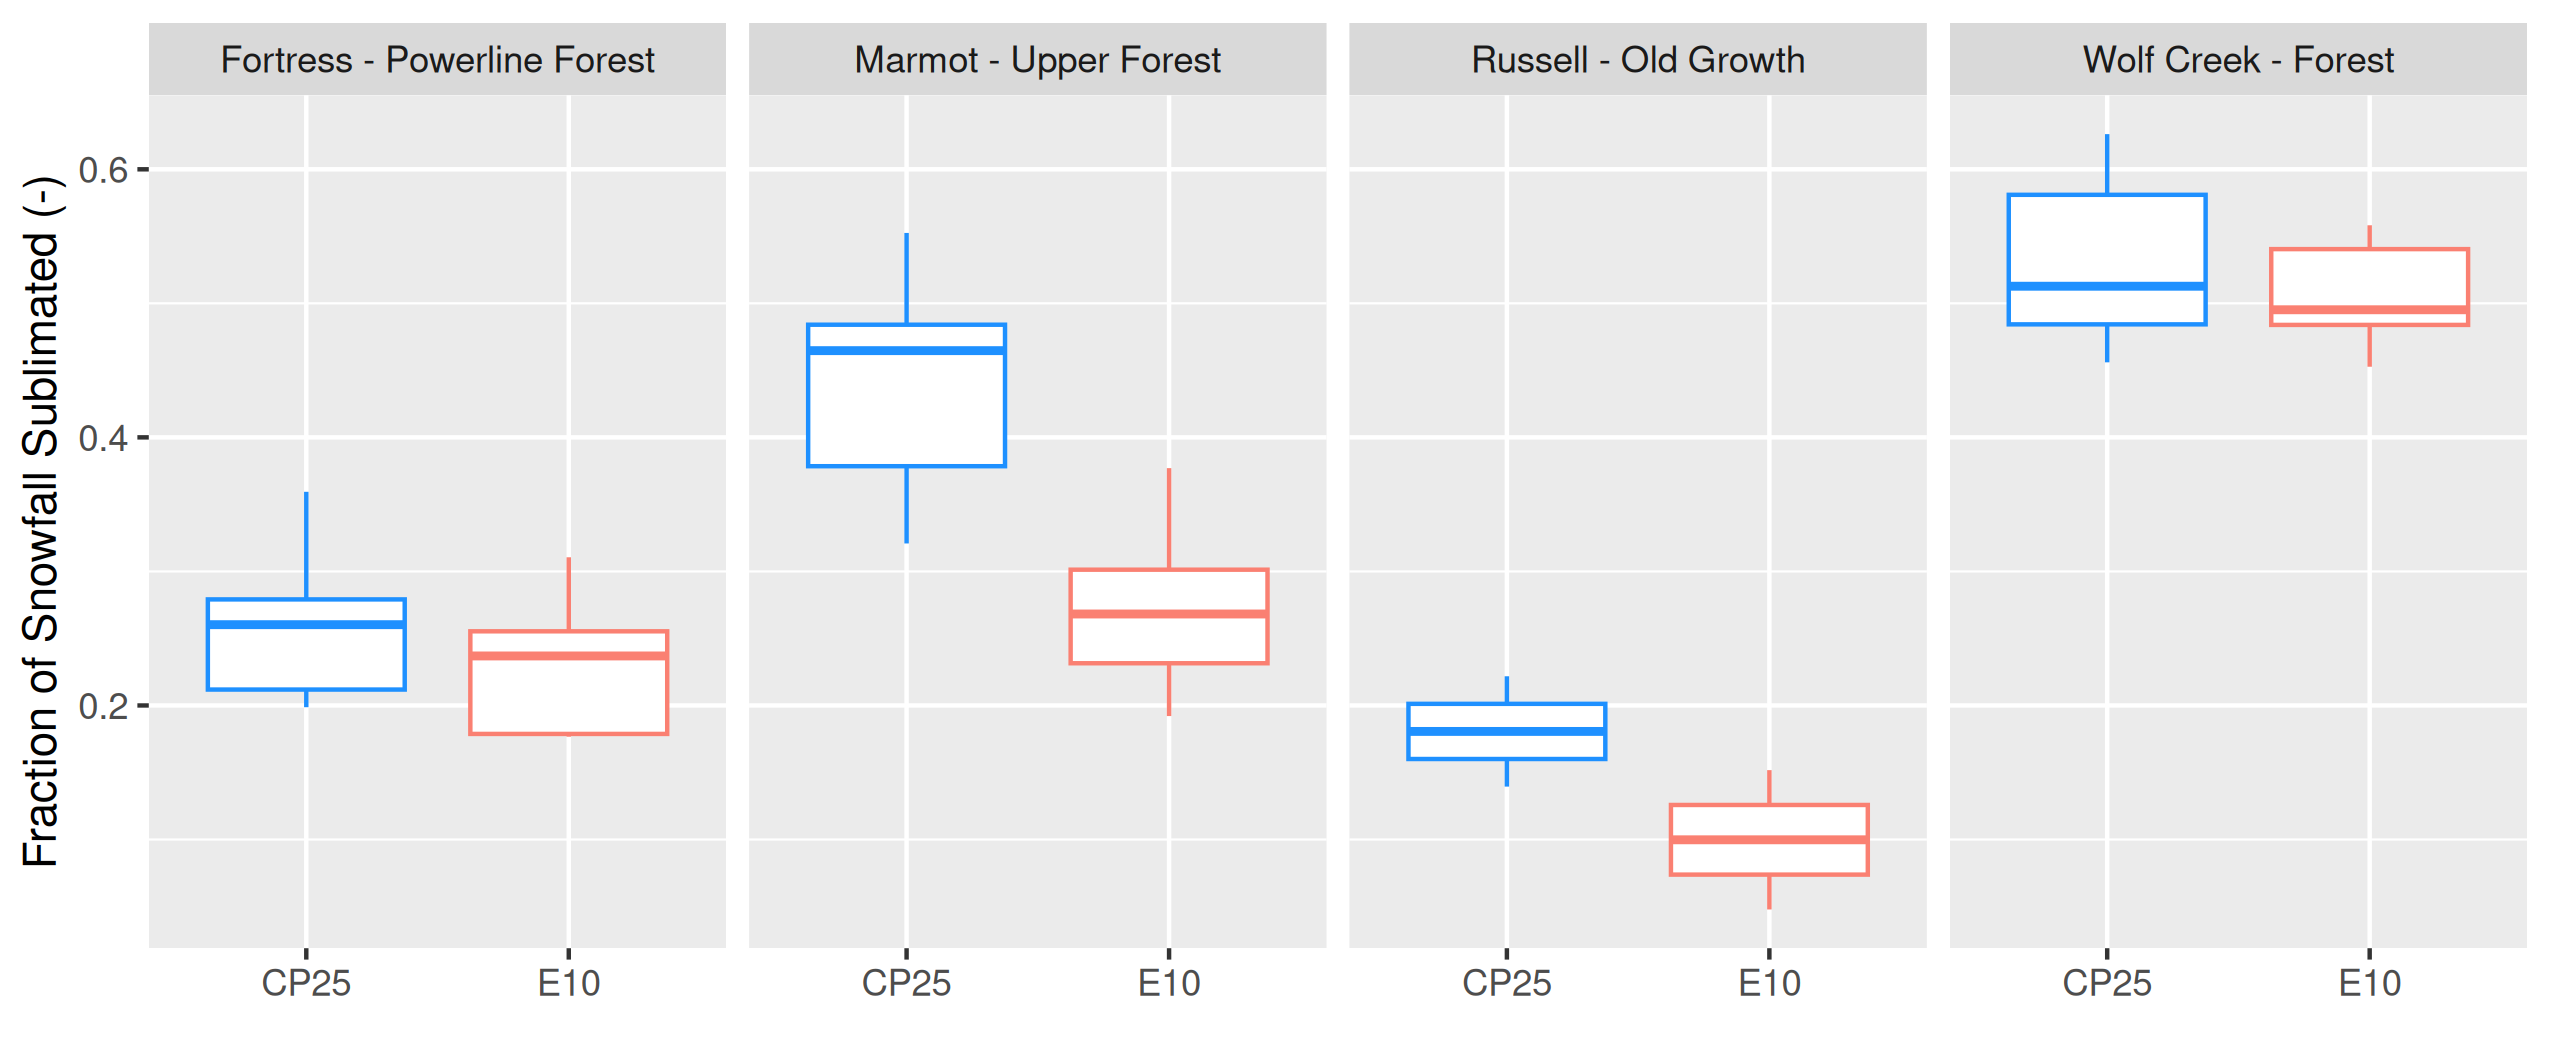
\includegraphics[keepaspectratio]{chapters/05-model-eval-paper/figs/figure6.png}}

}

\caption{\label{fig-frac-subl}Boxplots showing the distribution of the
fraction of total atmospheric snowfall that was sublimated out of the
canopy at each station. Note: the rectangle vertical extent represents
the interquartile range (25\textsuperscript{th} to
75\textsuperscript{th} percentile), the horizontal line within each box
indicates the median, and the whiskers extend to 1.5 times the
interquartile range. Circular points beyond the whiskers represent
outliers.}

\end{figure}%

\begin{figure}

\centering{

\pandocbounded{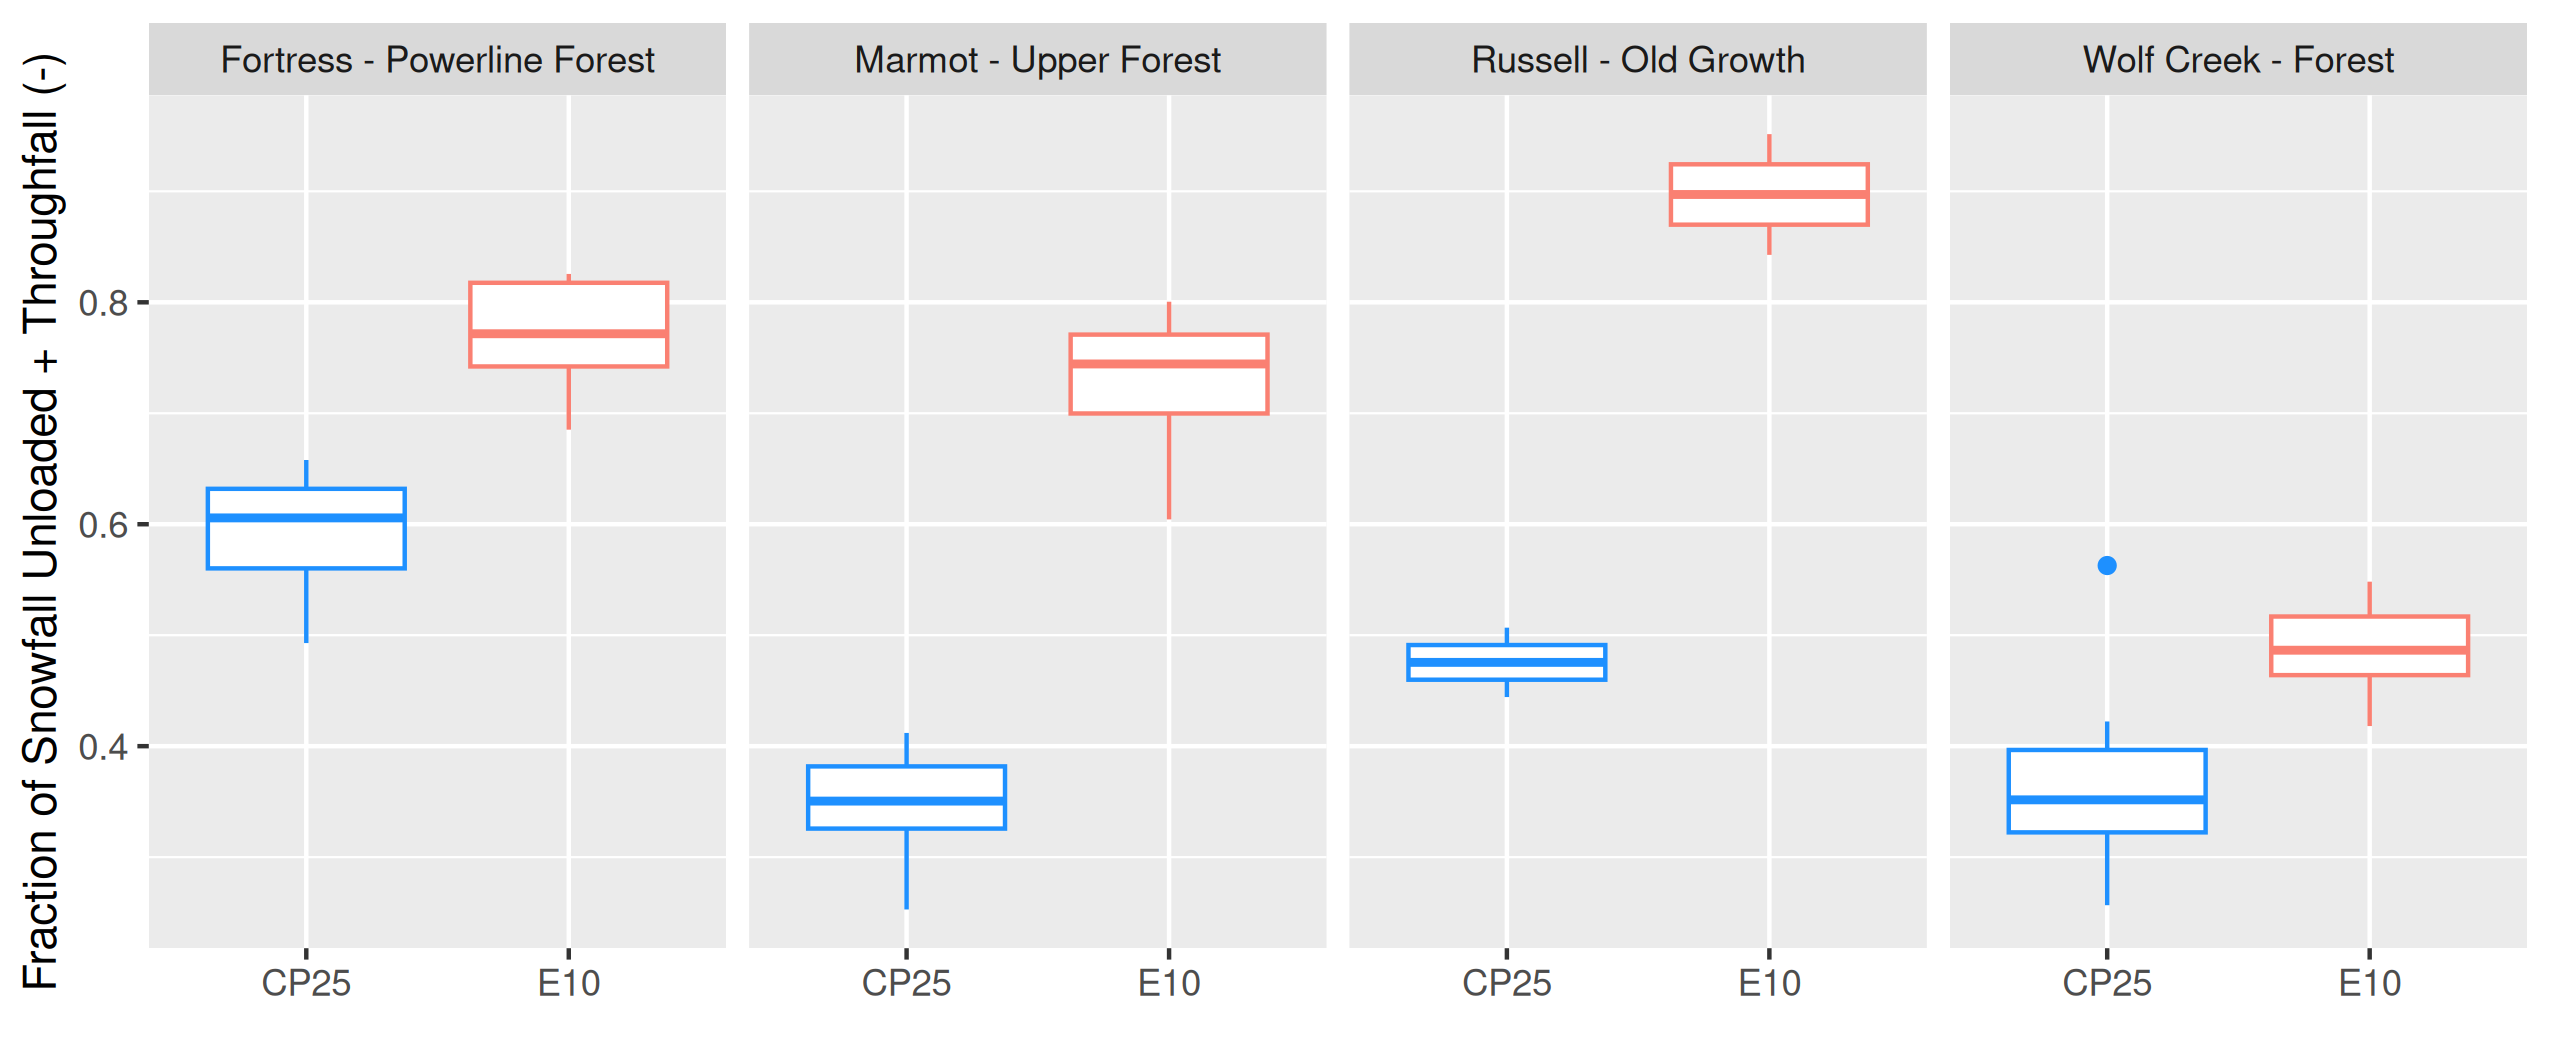
\includegraphics[keepaspectratio]{chapters/05-model-eval-paper/figs/figure7.png}}

}

\caption{\label{fig-frac-unld}Boxplots showing the distribution of the
fraction of total atmospheric snowfall that reached the subcanopy via
unloading and/or throughfall. Note: the rectangle vertical extent
represents the interquartile range (25\textsuperscript{th} to
75\textsuperscript{th} percentile), the horizontal line within each box
indicates the median, and the whiskers extend to 1.5 times the
interquartile range. Circular points beyond the whiskers represent
outliers.}

\end{figure}%

\begin{figure}

\centering{

\pandocbounded{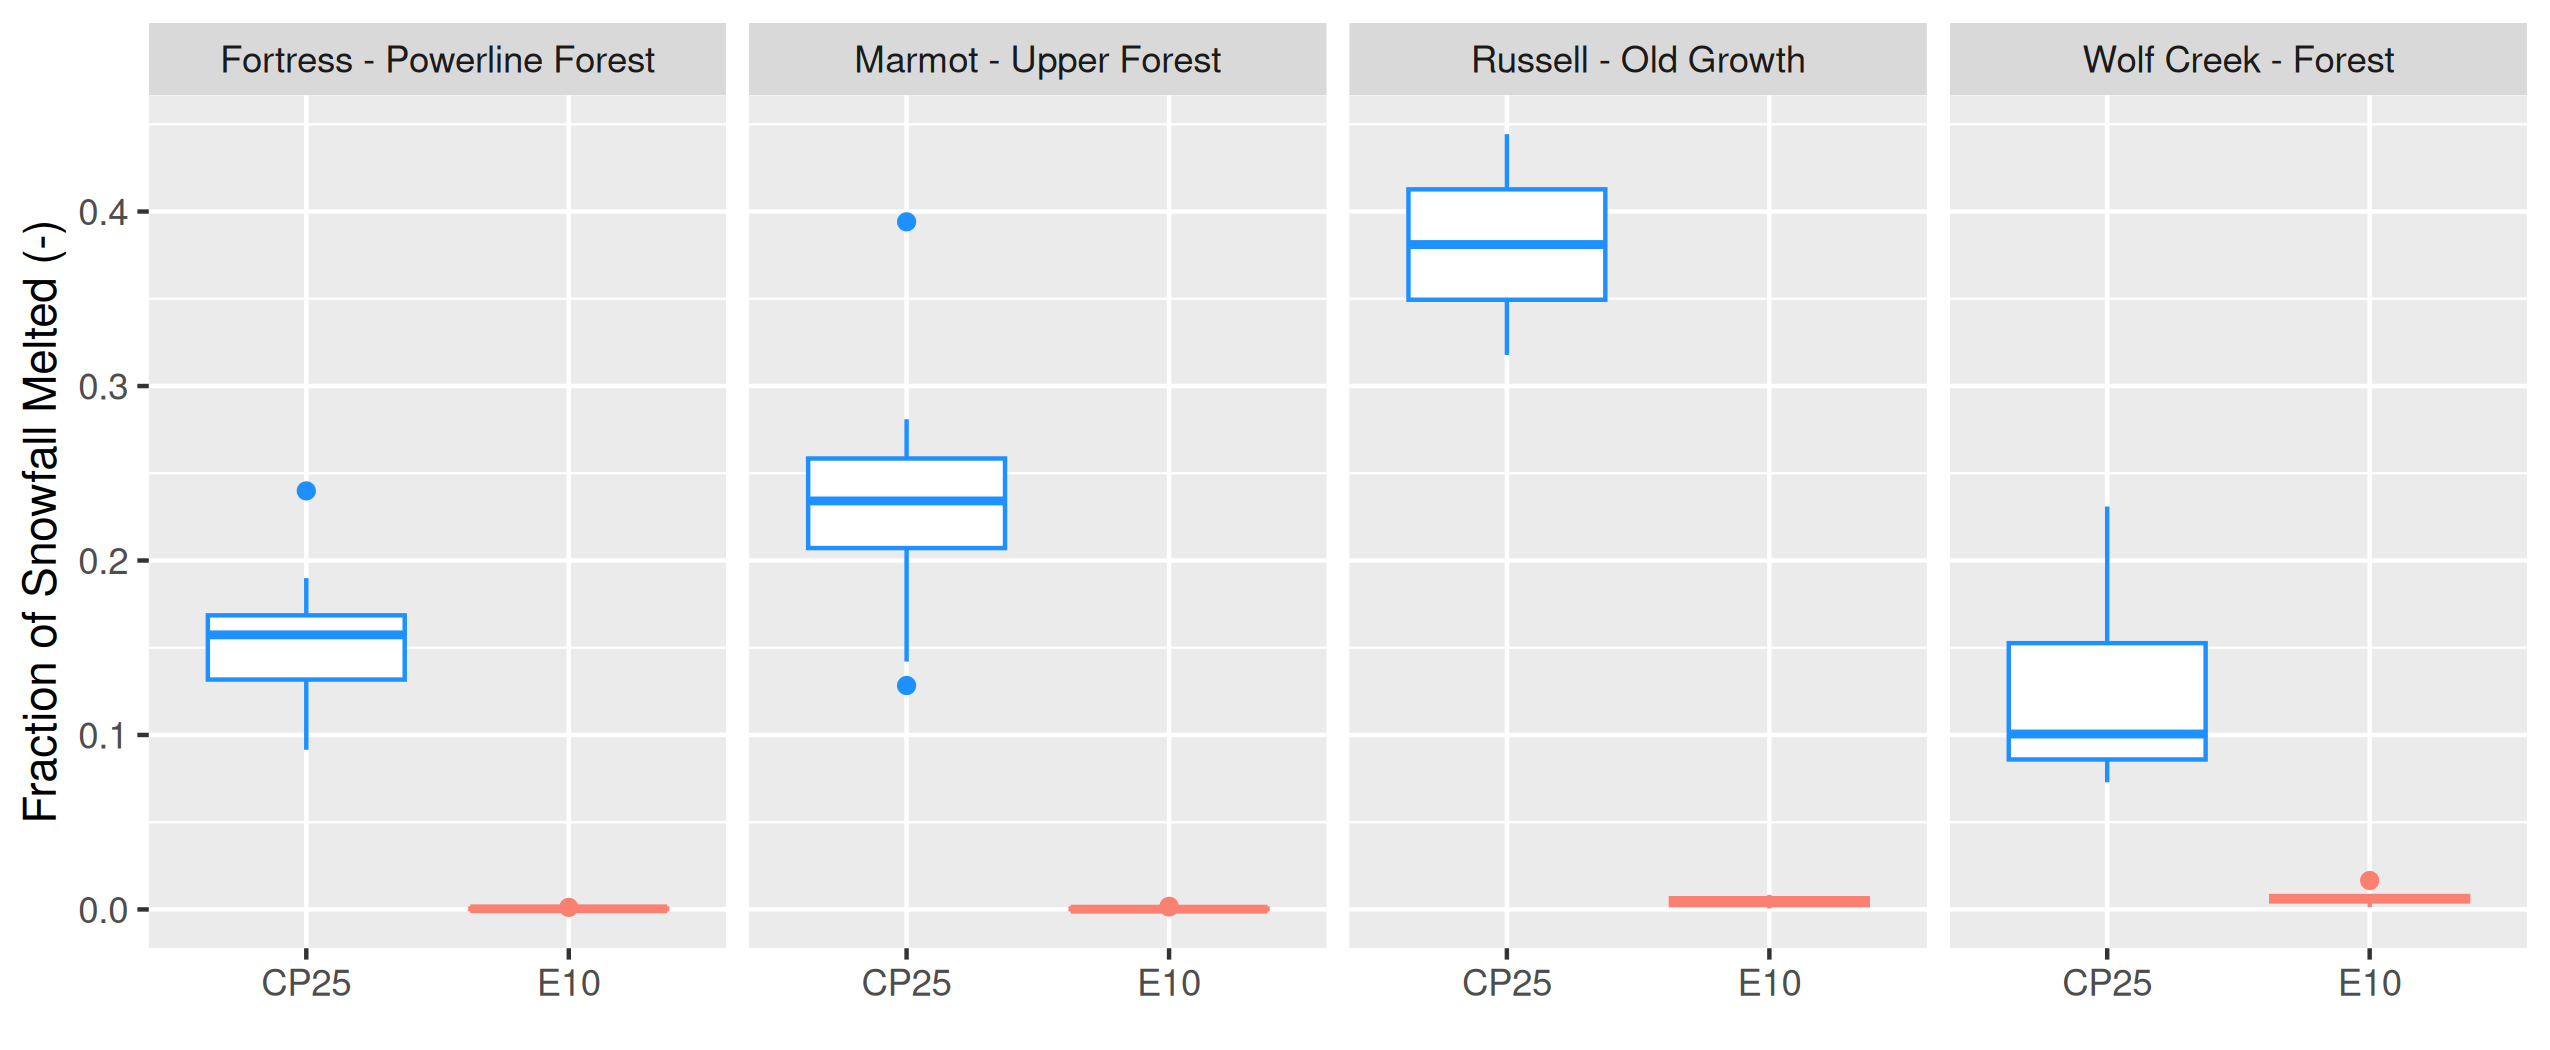
\includegraphics[keepaspectratio]{chapters/05-model-eval-paper/figs/figure8.png}}

}

\caption{\label{fig-frac-drip}Boxplots showing the distribution of the
fraction of total atmospheric snowfall that was melted out of the canopy
at each station. Note: the rectangle vertical extent represents the
interquartile range (25\textsuperscript{th} to 75\textsuperscript{th}
percentile), the horizontal line within each box indicates the median,
and the whiskers extend to 1.5 times the interquartile range. Circular
points beyond the whiskers represent outliers.}

\end{figure}%

\subsection{Simulated Canopy Snow
Load}\label{simulated-canopy-snow-load}

Over all years and sites, CP25 predicted consistently higher canopy snow
loads compared to the E10 model (Figure~\ref{fig-cpy-swe}). This results
from E10's increase in throughfall with increasing antecedent snow load
as well as the constant unloading rate as a function of snow load and
ice-bulb temperature and led to more snowfall partitioned to the ground
as solid snow compared to CP25 (Figure~\ref{fig-frac-unld}). Some
snowfall events had similar initial accumulation of snow in the canopy
between the two models up until the E10 species snow load capacity was
reached (see colder events in Jan and Feb at Fortress, Marmot, and Wolf
Creek in Figure~\ref{fig-cpy-swe-select}). Canopy snow load infrequently
reached the CP25 maximum load of 50 kg m\textsuperscript{-2} at all four
sites (Figure~\ref{fig-cpy-swe}). At Russell, while annual snowfall
amounts were similar to Fortress (Figure~\ref{fig-sf-subcpy-swe}),
increased canopy snow ablation rates due to warmer temperatures at
Russell limited the accumulation of snow in the canopy in spring
(Figure~\ref{fig-cpy-swe}; Figure~\ref{fig-cpy-swe-select}).

\begin{figure}

\centering{

\pandocbounded{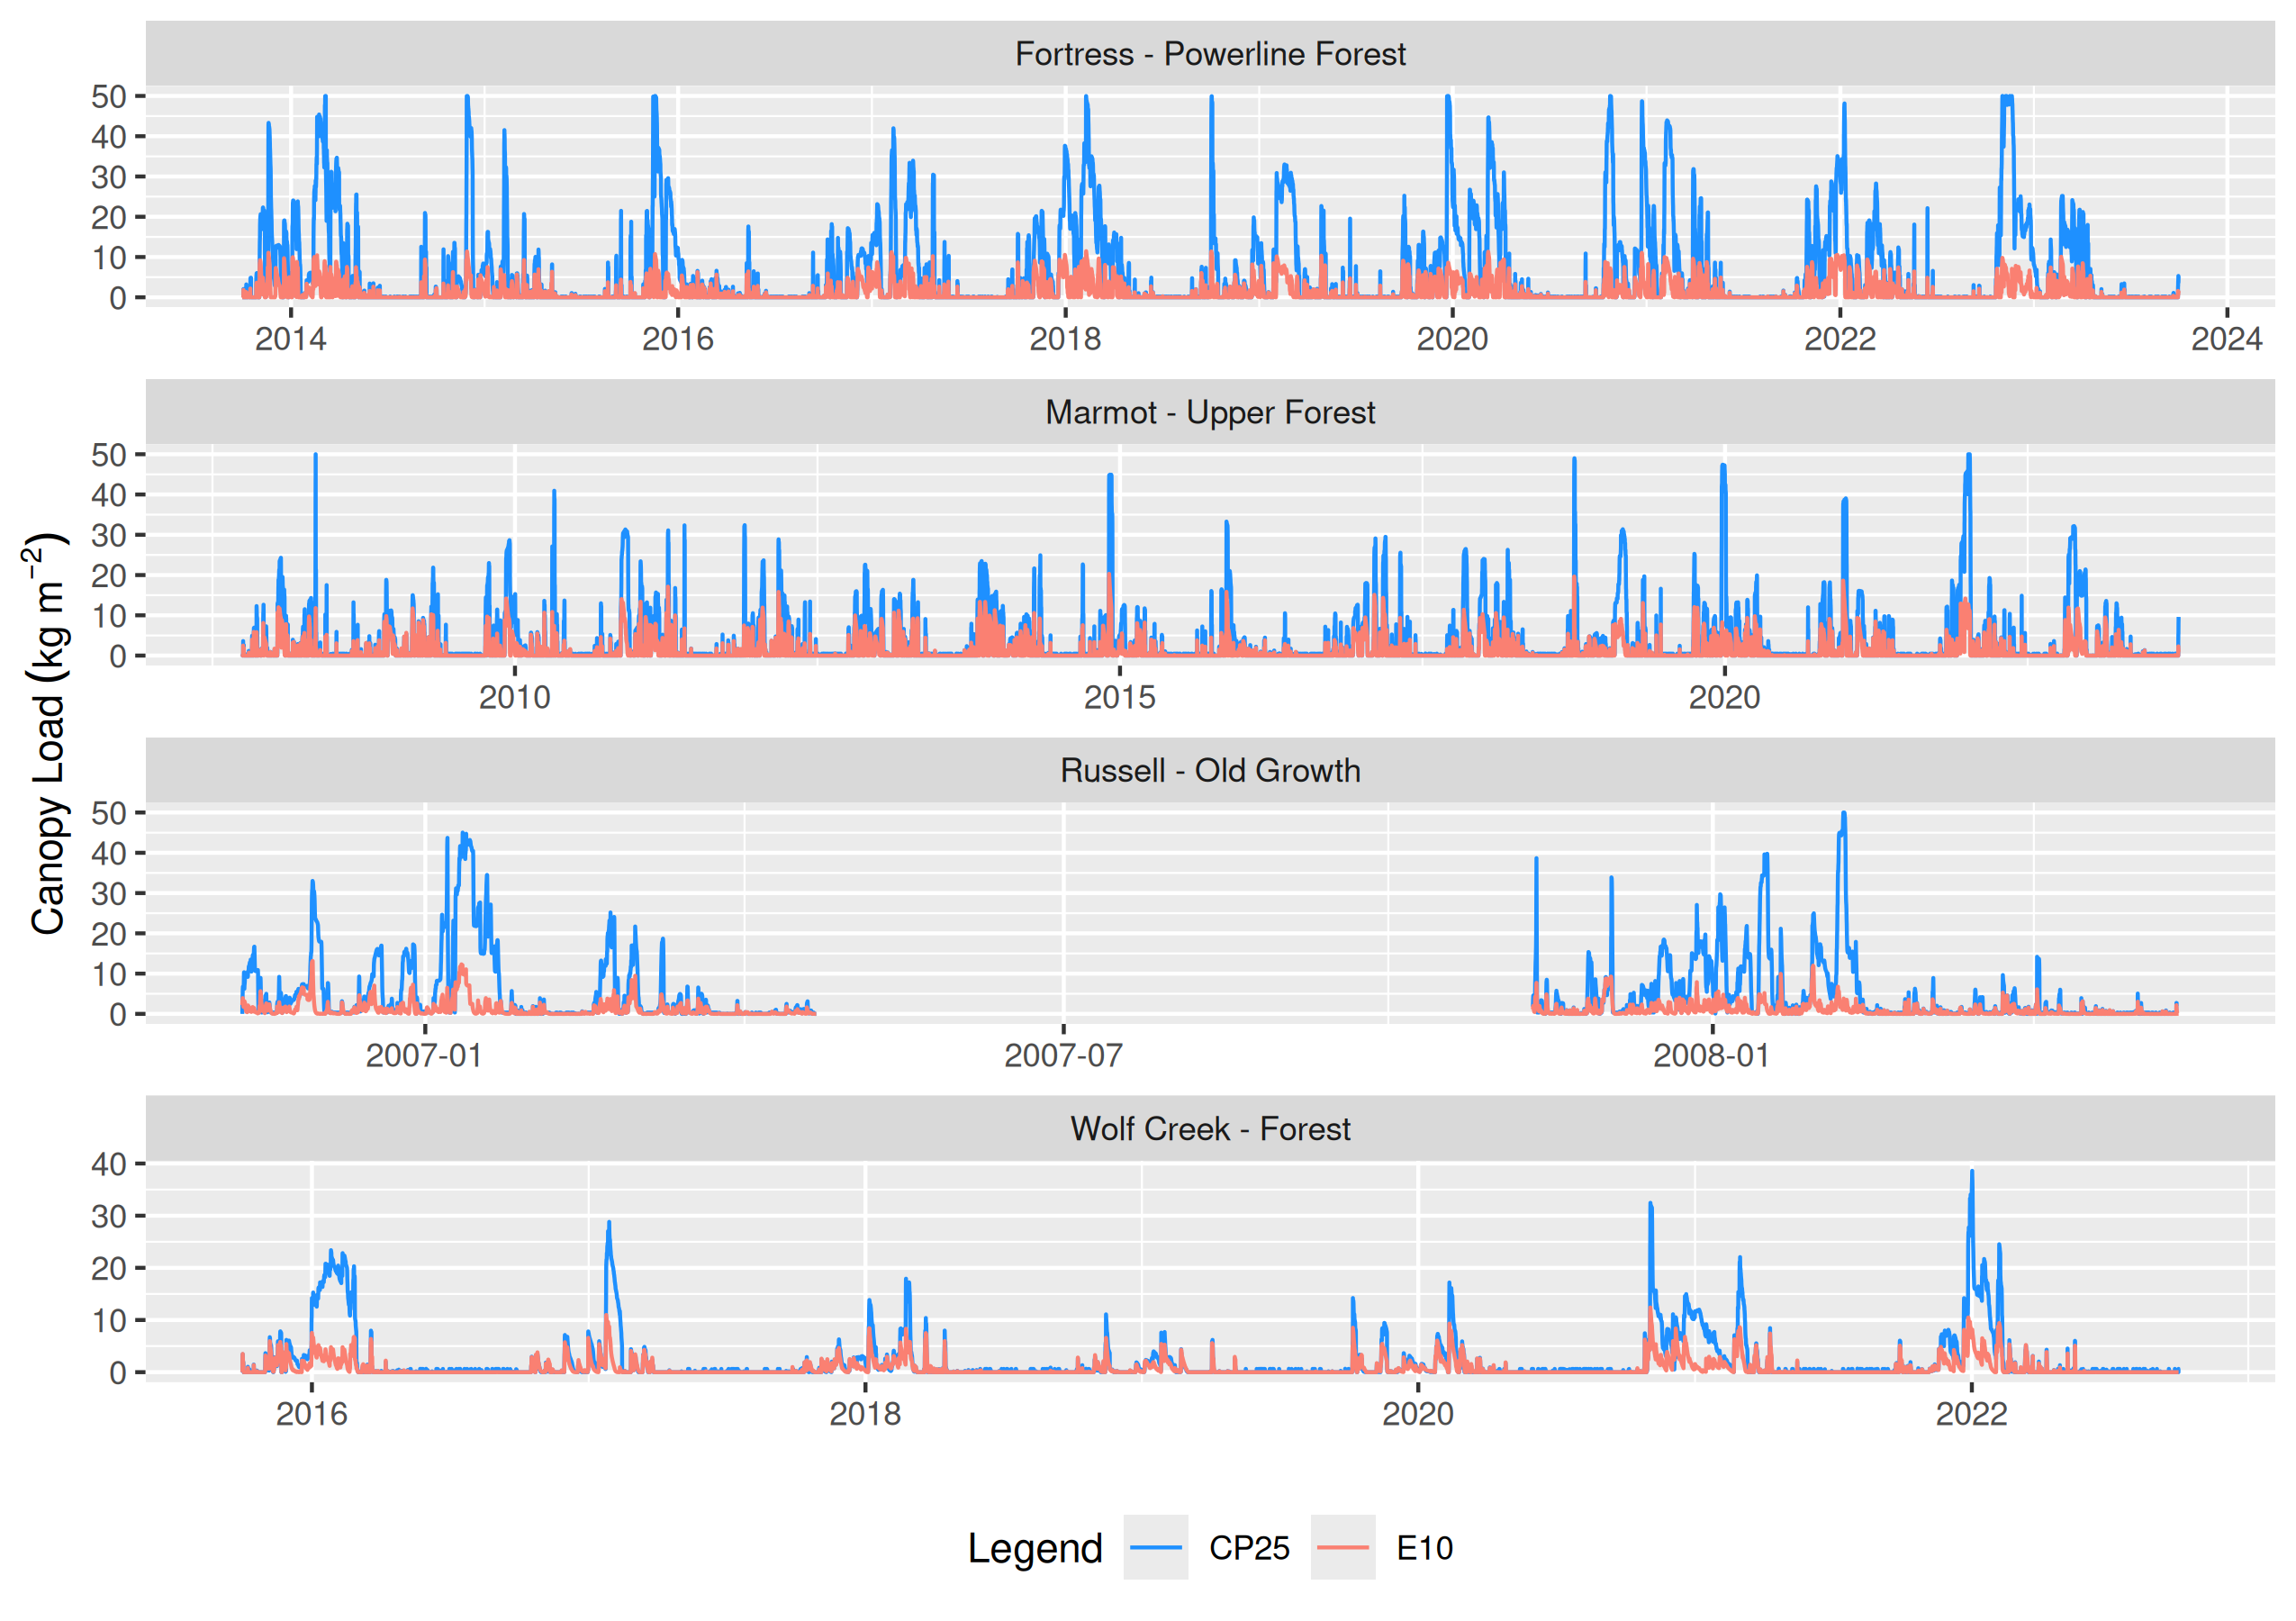
\includegraphics[keepaspectratio]{chapters/05-model-eval-paper/figs/figure9.png}}

}

\caption{\label{fig-cpy-swe}Timeseries of simulated canopy load for CP25
and E10 at each station for the full simulation period.}

\end{figure}%

\begin{figure}

\centering{

\pandocbounded{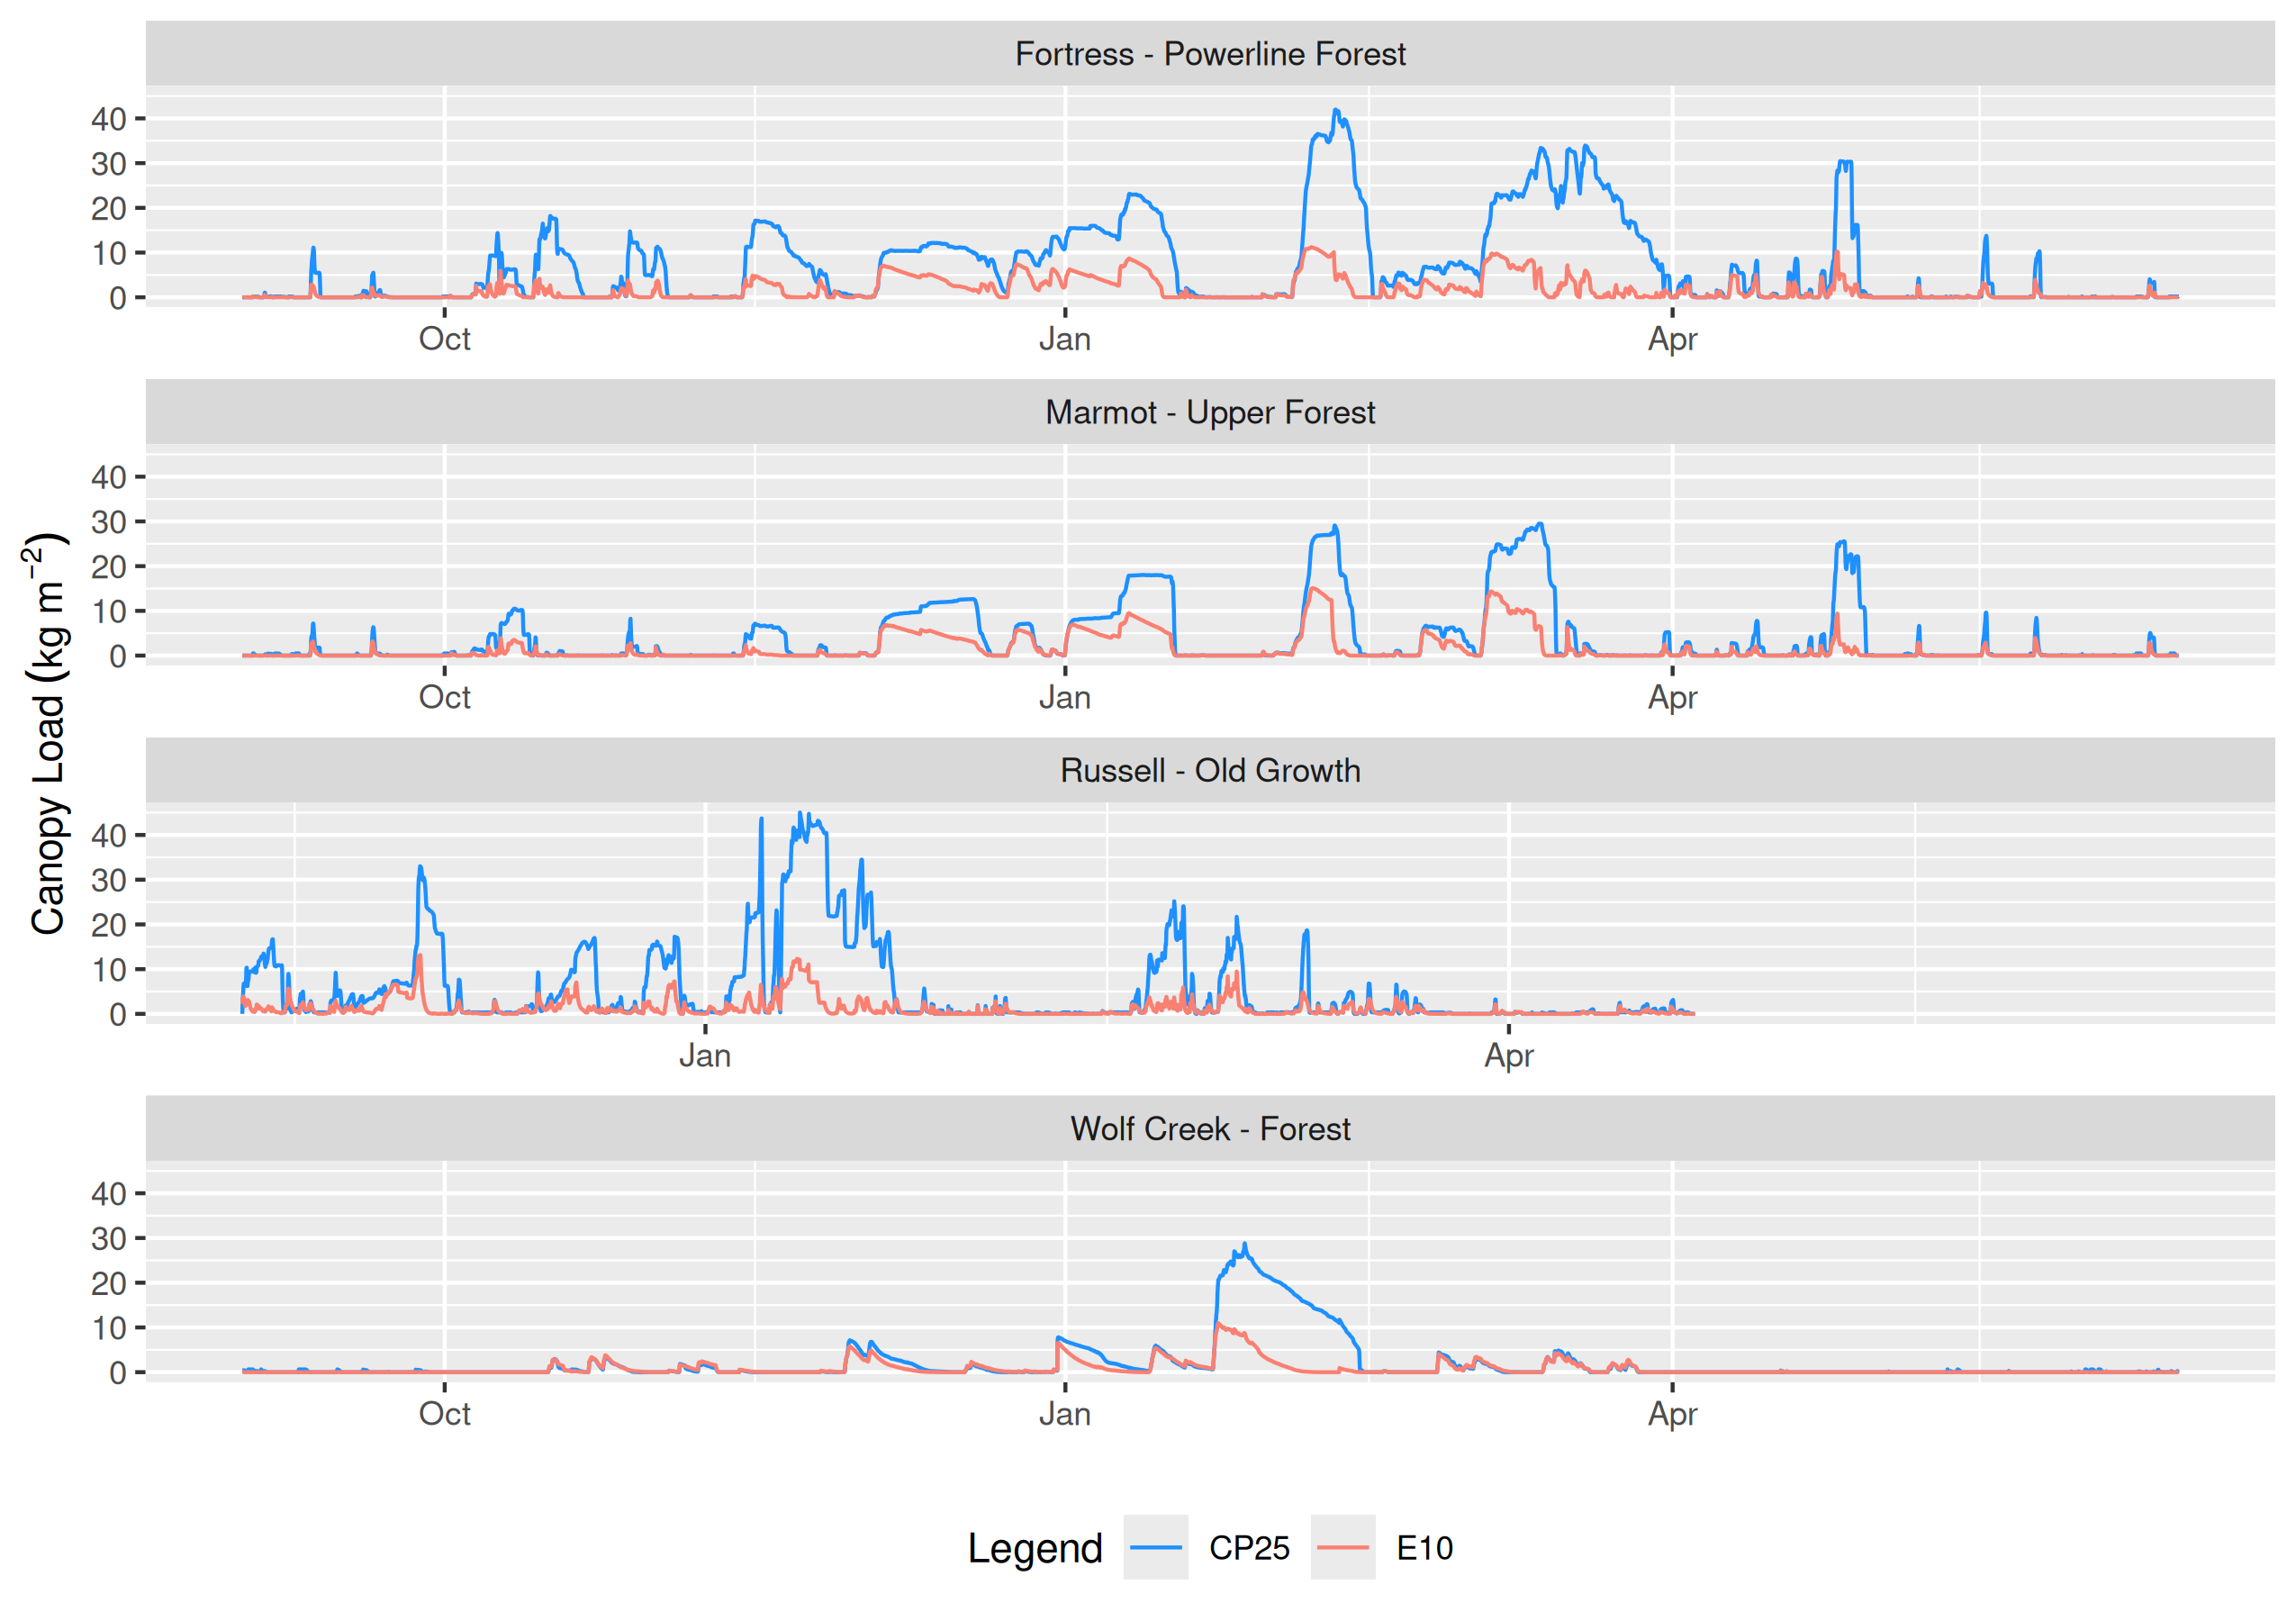
\includegraphics[keepaspectratio]{chapters/05-model-eval-paper/figs/figure10.png}}

}

\caption{\label{fig-cpy-swe-select}Timeseries of simulated canopy load
for CP25 and E10 at each station for select water years. The water year
2017 was selected for Fortress, Marmot, and Wolf Creek, while 2007 was
selected for Russell.}

\end{figure}%

In addition to the large difference in canopy load simulated between
CP25 and E10 across all four sites, the duration that the canopies of
each site were simulated to have more than 2 kg m\textsuperscript{-2} of
snow varied between the four sites and two models
(Figure~\ref{fig-frac-cpy-load-th}). A threshold of 2 kg
m\textsuperscript{-2} was selected based on observations by Pomeroy \&
Dion (1996) who found minimal influence of canopy snow load on above
canopy albedo for loads less than 1.6 kg m\textsuperscript{-2}. Across
all four sites, canopy loads greater than 2 kg m\textsuperscript{-2}
were observed to persist longer for CP25 compared to E10
(Figure~\ref{fig-frac-cpy-load-th}). At Fortress and Russell snow loads
above this threshold persisted up to two times longer for CP25 compared
to E10. The difference at Marmot and Wolf Creek between the two models
were found to be less due to the lower snowfall of these sites which
lowered event canopy snow loads thus yielding higher interception
inefficiencies for the E10 model.

\begin{figure}

\centering{

\pandocbounded{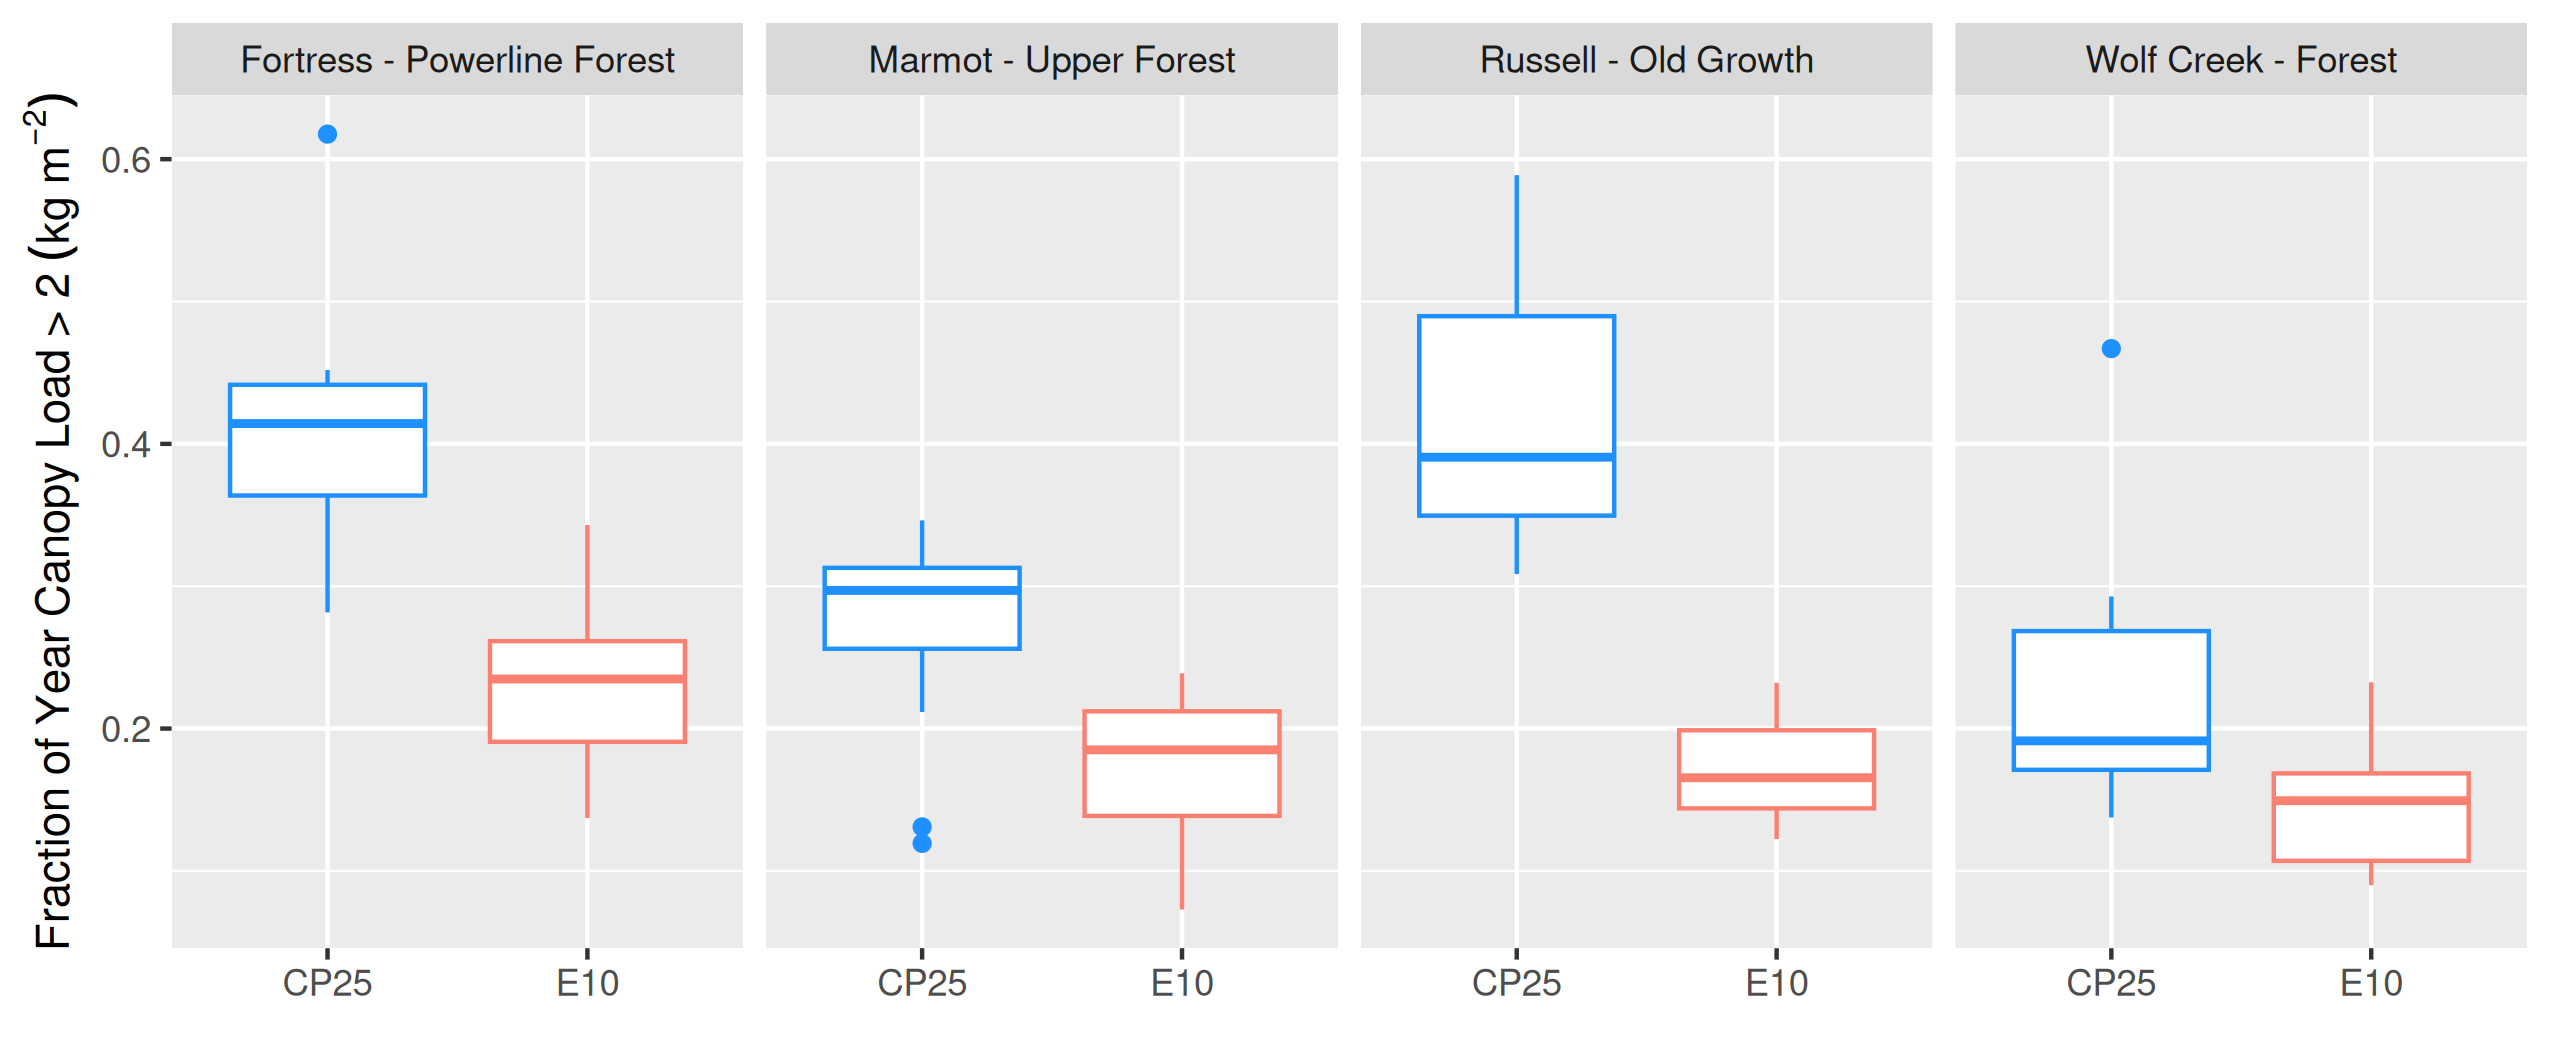
\includegraphics[keepaspectratio]{chapters/05-model-eval-paper/figs/figure11.png}}

}

\caption{\label{fig-frac-cpy-load-th}Boxplots showing the annual
fraction of time where simulated canopy snow load is greater than 2 kg
m\textsuperscript{-2} by the CP25 and E10 models.}

\end{figure}%

\section{Discussion}\label{discussion-3}

\subsection{Model Performance in Simulating Subcanopy Snow
Accumulation}\label{model-performance-in-simulating-subcanopy-snow-accumulation}

New parameterisations of the canopy snow energy and mass
balance---supported by advances in process understanding (Cebulski \&
Pomeroy, 2025b; Cebulski \& Pomeroy, 2025c; Lumbrazo et al., 2022;
Lundquist et al., 2021; Staines \& Pomeroy, 2023)---were evaluated for
their ability to simulate subcanopy SWE across a broad range of climate
and forest types. The higher canopy snow loads simulated by CP25 are
consistent with empirical observations (Calder, 1990; Cebulski \&
Pomeroy, 2025b; Hedstrom \& Pomeroy, 1998; Storck et al., 2002; Watanabe
\& Ozeki, 1964), which demonstrate a linear increase in interception
with snowfall without evidence of reaching a maximum capacity. By
calculating throughfall as a function of canopy density (Cebulski \&
Pomeroy, 2025b; Staines \& Pomeroy, 2023) and combining this with a
comprehensive canopy snow ablation routine (Cebulski \& Pomeroy, 2025c;
Lundquist et al., 2021), CP25 resulted in much larger intercepted snow
loads compared to E10. Consequently, E10 underestimated subcanopy SWE,
as less intercepted snow was exposed to sublimation or melt
(Table~\ref{tbl-swe-mb}).

Inclusion of both dry- and melt-induced unloading of canopy snow is
supported by observations (Cebulski \& Pomeroy, 2025c; Ellis et al.,
2010; Floyd, 2012; Lumbrazo et al., 2022; Roesch et al., 2001), with
mechanisms such as bond weakening, lubrication during melt, and wind
shear reinforcing their physical basis. An energy balance-based canopy
melt routine---recommended by many studies (Andreadis et al., 2009;
Cebulski \& Pomeroy, 2025c; Lumbrazo et al., 2022; Lundquist et al.,
2021; Storck et al., 2002)---improved representation of ablation under
warm conditions (Cebulski \& Pomeroy, 2025c) and likely contributed to
reduced error in subcanopy SWE simulations in this study at the
temperate-maritime Russell site. In contrast, the ice-bulb
temperature-based melt threshold (\textgreater{} 6 °C) was infrequently
reached and caused unloading to occur mainly as solid snow. While
accounting for wind-driven unloading reduced errors slightly in colder
sites, the largest improvements were at Russell, where CP25 better
captured canopy melt and drip.

Both models performed best at the sites where they were originally
developed (CP25 at Fortress and E10 at Marmot), which aligns with
observations by Lumbrazo et al. (2022) that parameters for unloading are
site specific and may suggest the initial interception parameters are as
well. Low error at the cold sites suggests that the dry snow unloading
parameterisation is transferable across sites and is consistent with
observations by Lumbrazo et al. (2022)---where a wind-driven unloading
parameterisation had good accuracy across a cold-climate sites. The CP25
model performed worst at the temperate-maritime Russell site, where
melt/drip and melt-induced unloading processes dominated, despite
showing improvements over E10 in this study and showing strong
performance over warm melt-driven events in Cebulski \& Pomeroy (2025c).
Remaining error at Russell may reflect unrepresented processes, such as
rime-ice accumulation observed in other maritime forests (Lumbrazo et
al., 2022), which increases canopy loads and alters partitioning into
liquid water. Additional uncertainties stem from simplifications in the
canopy energy balance (e.g., radiation transmittance, longwave emission,
and turbulent fluxes), as well as parameterisations of interception and
unloading (Cebulski \& Pomeroy, 2025b; Cebulski \& Pomeroy, 2025c).
These issues are likely amplified at Russell, where frequent air
temperatures near the melting point increase sensitivity to energy
balance formulations, compared to the colder sites with more stable
conditions.

Across the three colder sites, mean bias differed by less than 10 kg
m\textsuperscript{-2} between models, yet CP25 simulated longer periods
of canopy snow loads greater than 2 kg m\textsuperscript{-2}. This has
implications for improving the representation of above-canopy albedo in
land surface models which have previously shown poor performance with
existing canopy snow ablation models (Thackeray et al., 2014; Wang et
al., 2016). Moreover, E10's performance varied substantially between
years; it overestimated SWE over most years, but underestimated SWE in
low-snowfall years when reduced unloading rates allowed more sublimation
(e.g., Marmot in 2019; Figure~\ref{fig-swe-ann-mean}).

These results show that recent process-based
parameterisations---particularly the treatment of canopy load, ablation,
and unloading---yield measurable improvements in simulating subcanopy
SWE across diverse climates and forest types, and have direct
implications for representation of surface albedo in land-surface
schemes.

\subsection{Influence of Climate on Snowfall
Partitioning}\label{influence-of-climate-on-snowfall-partitioning}

Although Russell and Fortress received similar amounts of snowfall
(Figure~\ref{fig-sf-subcpy-swe}), subcanopy accumulation was lower at
Russell due to enhanced canopy ablation: \textasciitilde40\% of annual
snowfall melted and 20\% sublimated in the canopy, compared to
\textasciitilde35\% combined losses at Fortress. The low cold content of
the maritime snowpack at Russell led to canopy snow drip rarely
refreezing, and warmer air temperatures (Figure~\ref{fig-met-normals})
further promoted melt throughout the season (Figure~\ref{fig-swe-ts}).
The prevalence of snowmelt both in the canopy and on the ground at
Russell led to the lowest fraction of seasonal snowfall stored in the
subcanopy (0.3) at peak SWE.

At Fortress, colder conditions, higher snowfall, and greater wind
exposure increased unloading rates, limited sublimation despite the
meteorological conditions favourable for it
(Figure~\ref{fig-frac-subl}). Combined with low canopy melt
(Figure~\ref{fig-frac-drip}), these processes yielded the highest
subcanopy storage fraction (0.6) across all four sites.

Marmot and Wolf Creek experienced cooler, drier conditions and lower
snowfall, leading to reduced unloading and a greater role of sublimation
in canopy losses (Figure~\ref{fig-frac-subl}). Canopy melt played only a
minor role, but high sublimation fractions meant that only
\textasciitilde0.4 of snowfall remained in the subcanopy snowpack at
peak SWE. Simulated sublimation for these two sites (\textasciitilde50\%
of seasonal snowfall; Figure~\ref{fig-frac-subl}) exceeded the upper
range of global estimates (25--45\%) reported by Essery et al. (2003)
but is consistent with observations by Pomeroy \& Gray (1995) and Ellis
et al. (2010).

Despite storing the smallest fraction of snowfall, Russell delivered the
greatest amount of water to the soil because most canopy ablation
occurred as melt and solid snow unloading rather than sublimation.
Relatively consisting mid winter melt of snow in the canopy provided a
steady year-round input of liquid water, which could contribute to the
longer vegetation growing season and may enhance groundwater recharge.
Previous studies (Barnhart et al., 2016; Hayashi, 2020) highlight that
slow, sustained melt increases infiltration opportunity, whereas rapid
melt promotes runoff. In contrast, colder sites with fewer mid-winter
melt events may partition a greater fraction of precipitation into
runoff.

\subsection{Influence of Tree Species on Snowfall
Partitioning}\label{influence-of-tree-species-on-snowfall-partitioning}

The species of needleleaf forest overlying each site also influenced
subcanopy SWE accumulation. However, limited research has been conducted
on how branches elasticity, needle composition, and crown structure
affect both the interception and ablation of snow in the canopy. The
Marmot and Wolf Creek sites both were primarily composed of spruce trees
(Table~\ref{tbl-site-meta}) and exposed to similarly cool climates
(Figure~\ref{fig-met-normals}), showed comparable fractions of snowfall
stored in the subcanopy and similar canopy melt and sublimation losses
(Figure~\ref{fig-frac-drip}; Figure~\ref{fig-frac-subl}).

In contrast, Fortress and Russell were both primarily fir-dominated
forests, yet diverged strongly due to climate differences
(Figure~\ref{fig-met-normals}) and vegetation structure. Despite only
\textasciitilde20\% greater canopy cover, Russell stored about half the
fraction of snowfall in the subcanopy compared to Fortress. Tree size is
a likely factor: large 50 m tall fir trees at Russell can intercept far
more snow than the smaller 10 m fir trees at Fortress. Coupled with low
winds, this increased exposure of intercepted snow to canopy energy
fluxes favored melt and drip at Russell. The larger, more supportive
branches may also have slowed unloading, contributing to CP25's
overestimate of subcanopy SWE at Russell.

These results support earlier theory by Satterlund \& Haupt (1970) that
vegetation structure, density, and climate exert stronger control on
forest--snow partitioning than needleleaf species alone. However, other
forest types, such as broadleaf deciduous or cedar stands, have less
supportive branches and different needle or leaf structures, and are
therefore expected to exert a stronger influence on canopy--snow
processes than the relatively subtle species differences observed among
needleleaf sites in this study.

\section{Conclusions}\label{conclusions-3}

This study shows that advances in the representation of canopy snow
energy and mass balance can substantially improve the snowpack
simulations across forests spanning a range of climates and canopy
structures. The new physically based canopy snow model reduced errors in
simulating subcanopy snowpacks and provided new opportunities to
diagnose the processes that govern how snowfall is partitioned between
the atmosphere, canopy, and forest floor. Building on recent
developments, the new approach replaced earlier theories on the
assumption of a maximum canopy snow load with an interception
calculation based on canopy density, and represented ablation more
explicitly through melt- and wind-driven unloading, energy
balance--based melt and drip, and sublimation processes that vary with
canopy snow load. Compared with an existing model, the revised approach
more accurately represented the melt of intercepted snow, particularly
in the coastal--maritime environment, where errors in subcanopy SWE were
an order of magnitude lower. These results highlight the robustness of
physically based parameterisations under warm conditions, which is
particularly important given that continued warming may reduce the
applicability of empirically derived routines.

Process diagnosis conducted using the new approach highlighted the role
of vegetation in controlling snowfall partitioning. The greatest
influence was observed in the temperate--maritime forest, where high
energy input to intercepted snow caused nearly half of seasonal snowfall
to melt within the canopy, producing the lowest subcanopy SWE fraction
and a steady contribution of meltwater throughout the winter. Despite
the large influence of vegetation on the subcanopy snowpack, sublimation
losses were relatively small (\textasciitilde20\% of seasonal snowfall)
due to high humidity. At two cold continental sites with lower annual
snowfall, reduced unloading allowed a larger proportion of intercepted
snow to be lost to sublimation (\textasciitilde50\%). In contrast, the
cold wind-exposed site with higher snowfall exhibited greater unloading,
which limited sublimation losses relative to the other cold sites.
Overall, climate and canopy density exerted stronger controls on
seasonal snowfall partitioning than species-level differences among fir-
and spruce-dominated forests.

Although the new model simulated subcanopy SWE well, uncertainties
remain in partitioning of snowfall between sublimation losses and liquid
water inputs to the forest floor, as direct flux measurements have only
been validated at one site in a previous study. Measurements of snow
interception, unloading, drip, and sublimation are rarely made at
hydrometeorological stations but would provide important data to
evaluate and refine process-level representations across differing
environments. Further research is also needed to determine how unloading
depends on intercepted snow load, as this relationship is likely to vary
with both climate and tree characteristics. Greater cohesion and
adhesion in humid climates and more supportive branch and needle
structures in certain species may influence how snow is retained or shed
from canopies. Improved process-level measurements, combined with
continued model development, will help to identify these uncertainties
and support the transferability of canopy snow models across the wide
range of conditions found in cold-region forests.

\section{Acknowledgements}\label{acknowledgements-1}

We acknowledge financial support from the University of Saskatchewan
Dean's Scholarship, the Natural Sciences and Engineering Research
Council of Canada's Discovery Grants, the Canada First Research
Excellence Fund's Global Water Futures Programme, Environment and
Climate Change Canada, Alberta Innovates Water Innovation Program, the
Canada Foundation for Innovation's Global Water Futures Observatories
facility, and the Canada Research Chairs Programme. We thank Hannah
Koslowsky, Kieran Lehan, Lindsey Langs, Rosy Tutton, David Barrett, and
Tyler De Jong for their help in the field and Tom Brown and Logan Fang
for support of the CRHM platform.

\section{Data and Sofware Availability
Statement}\label{data-and-sofware-availability-statement}

The Cold Regions Hydrological Model Platform (CRHM) source code is
available at https://github.com/srlabUsask/crhmcode. Model forcing data,
model outputs, validation data, processed data, and scripts to run the
processing are available at \_\_\_\_ .

\pagebreak

\bookmarksetup{startatroot}

\chapter*{References}\label{references}
\addcontentsline{toc}{chapter}{References}

\markboth{References}{References}

\phantomsection\label{refs}
\begin{CSLReferences}{1}{0}
\bibitem[\citeproctext]{ref-Allan1998}
Allan, R., Pereira, L., Raes, D., \& Smith, M. (1998). \emph{Crop
evapotranspiration {Guidelines} for computing crop water requirements}.
{Food and Agriculture Organization of the United Nations}.

\bibitem[\citeproctext]{ref-Andreadis2009}
Andreadis, K. M., Storck, P., \& Lettenmaier, D. P. (2009). Modeling
snow accumulation and ablation processes in forested environments.
\emph{Water Resources Research}, \emph{45}(5), 1--33.
\url{https://doi.org/10.1029/2008WR007042}

\bibitem[\citeproctext]{ref-Annandale2002}
Annandale, J., Jovanovic, N., Benadé, N., \& Allen, R. (2002). Software
for missing data error analysis of {Penman-Monteith} reference
evapotranspiration. \emph{Irrigation Science}, \emph{21}(2), 57--67.
\url{https://doi.org/10.1007/s002710100047}

\bibitem[\citeproctext]{ref-Aston1979}
Aston, A. R. (1979). Rainfall interception by eight small trees.
\emph{Journal of Hydrology}, \emph{42}(3-4), 383--396.
\url{https://doi.org/10.1016/0022-1694(79)90057-X}

\bibitem[\citeproctext]{ref-Aubry-Wake2023}
Aubry-Wake, C., \& Pomeroy, J. W. (2023). Predicting hydrological change
in an alpine glacierized basin and its sensitivity to landscape
evolution and meteorological forcings. \emph{Water Resources Research},
\emph{59}(9). \url{https://doi.org/10.1029/2022WR033363}

\bibitem[\citeproctext]{ref-Baggi2008}
Baggi, S., \& Schweizer, J. (2008). Characteristics of wet-snow
avalanche activity: 20 years of observations from a high alpine valley
({Dischma}, {Switzerland}). \emph{Natural Hazards}, \emph{50}(1),
97--108. \url{https://doi.org/10.1007/s11069-008-9322-7}

\bibitem[\citeproctext]{ref-Barnhart2016}
Barnhart, T. B., Molotch, N. P., Livneh, B., Harpold, A. A., Knowles, J.
F., \& Schneider, D. (2016). Snowmelt rate dictates streamflow.
\emph{Geophysical Research Letters}, \emph{43}(15), 8006--8016.
\url{https://doi.org/10.1002/2016gl069690}

\bibitem[\citeproctext]{ref-Bartlett2015}
Bartlett, P. A., \& Verseghy, D. L. (2015). Modified treatment of
intercepted snow improves the simulated forest albedo in the {Canadian
Land Surface Scheme}. \emph{Hydrological Processes}, \emph{29}(14),
3208--3226. \url{https://doi.org/10.1002/HYP.10431}

\bibitem[\citeproctext]{ref-Beria2018}
Beria, H., Larsen, J. R., Ceperley, N. C., Michelon, A., Vennemann, T.,
\& Schaefli, B. (2018). Understanding snow hydrological processes
through the lens of stable water isotopes. \emph{Wiley Interdisciplinary
Reviews: Water}, \emph{5}(6), 1--23.
\url{https://doi.org/10.1002/wat2.1311}

\bibitem[\citeproctext]{ref-Berndt1969}
Berndt, H. W., \& Fowler, W. B. (1969). Rime and hoarfrost in
upper-slope forests of eastern washington. \emph{Journal of Forestry},
\emph{67}(2), 92--95. \url{https://doi.org/10.1093/jof/67.2.92}

\bibitem[\citeproctext]{ref-Best2011a}
Best, M. J., Pryor, M., Clark, D. B., Rooney, G. G., Essery, R. L. H.,
Ménard, C. B., Edwards, J. M., Hendry, M. A., Porson, A., Gedney, N.,
Mercado, L. M., Sitch, S., Blyth, E., Boucher, O., Cox, P. M., Grimmond,
C. S. B., \& Harding, R. J. (2011). The {Joint UK Land Environment
Simulator} ({JULES}), model description -- {Part} 1: {Energy} and water
fluxes. \emph{Geoscientific Model Development}, \emph{4}(3), 677--699.
\url{https://doi.org/10.5194/gmd-4-677-2011}

\bibitem[\citeproctext]{ref-Betts1997}
Betts, A. K., \& Ball, J. H. (1997). Albedo over the boreal forest.
\emph{Journal of Geophysical Research: Atmospheres}, \emph{102}(D24),
28901--28909. \url{https://doi.org/10.1029/96JD03876}

\bibitem[\citeproctext]{ref-Brutsaert1982}
Brutsaert, W. (1982). \emph{Evaporation into the atmosphere: Theory,
history, and applications}. Dordrecht, Holland: Reidel.

\bibitem[\citeproctext]{ref-Bush2019}
Bush, E., \& Lemmen, D. S. (2019). \emph{Canada's changing climate
report} (p. 444). Government of Canada.

\bibitem[\citeproctext]{ref-Calder1990}
Calder, I. R. (1990). \emph{Evaporation in the uplands} (p. 148). Wiley.

\bibitem[\citeproctext]{ref-NALCMS2020}
Canada Centre for Remote Sensing, Canada Centre for Mapping and Earth
Observation, \& Canada, N. R. (2020). \emph{Land {Cover} of {North
America} at 30 meters} {[}Raster Digital Data{]}.

\bibitem[\citeproctext]{ref-Cebulski2025}
Cebulski, A. C., \& Pomeroy, J. W. (2025a). Theoretical {Underpinnings}
of {Snow Interception} and {Canopy Snow Ablation Parameterisations}.
\emph{WIREs Water}, \emph{12}, e70010.
\url{https://doi.org/10.1002/wat2.70010}

\bibitem[\citeproctext]{ref-Cebulski2025a}
Cebulski, A. C., \& Pomeroy, J. W. (2025b). Snow {Interception
Relationships With Meteorology} and {Canopy Density}. \emph{Hydrological
Processes}, \emph{39}(4), e70135.
\url{https://doi.org/10.1002/hyp.70135}

\bibitem[\citeproctext]{ref-Cebulski2025b}
Cebulski, A. C., \& Pomeroy, J. W. (2025c). Processes {Governing} the
{Ablation} of {Intercepted Snow}. \emph{Water Resources Research},
\emph{in review}.

\bibitem[\citeproctext]{ref-Chianucci2023}
Chianucci, F., \& Macek, M. (2023). {hemispheR}: An {R} package for
fisheye canopy image analysis. \emph{Agricultural and Forest
Meteorology}.

\bibitem[\citeproctext]{ref-Cionco1965}
Cionco, R. M. (1965). A mathematical model for air flow in a vegetative
canopy. \emph{Journal of Applied Meteorology (1962)}, \emph{4}(4),
517--522.
\url{https://doi.org/10.1175/1520-0450(1965)004\%3C0517:AMMFAF\%3E2.0.CO;2}

\bibitem[\citeproctext]{ref-Claassen1995}
Claassen, H. C., \& Downey, J. S. (1995). A {Model} for {Deuterium} and
{Oxygen} 18 {Isotope Changes During Evergreen Interception} of
{Snowfall}. \emph{Water Resources Research}, \emph{31}(3), 601--618.
\url{https://doi.org/10.1029/94WR01995}

\bibitem[\citeproctext]{ref-Clark2010a}
Clark, M. P., \& Kavetski, D. (2010). Ancient numerical daemons of
conceptual hydrological modeling: 1. {Fidelity} and efficiency of time
stepping schemes. \emph{Water Resources Research}, \emph{46}(10), 1--23.
\url{https://doi.org/10.1029/2009WR008894}

\bibitem[\citeproctext]{ref-Clark2015}
Clark, M. P., Nijssen, B., Lundquist, J. D., Kavetski, D., Rupp, D. E.,
Woods, R. A., Freer, J. E., Gutmann, E. D., Wood, A. W., Brekke, L. D.,
Arnold, J. R., Gochis, D. J., \& Rasmussen, R. M. (2015a). A unified
approach for process-based hydrologic modeling: 1. {Modeling} concept.
\emph{Water Resources Research}, \emph{51}(4), 2498--2514.
\url{https://doi.org/10.1002/2015WR017198}

\bibitem[\citeproctext]{ref-Clark2015b}
Clark, M. P., Nijssen, B., Lundquist, J. D., Kavetski, D., Rupp, D. E.,
Woods, R. A., Freer, J. E., Gutmann, E. D., Wood, A. W., Gochis, D. J.,
Rasmussen, R. M., Tarboton, D. G., Mahat, V., Flerchinger, G. N., \&
Marks, D. G. (2015b). A unified approach for process-based hydrologic
modeling: 2. {Model} implementation and case studies. \emph{Water
Resources Research}, \emph{51}(4), 2515--2542.
\url{https://doi.org/10.1002/2015WR017200}

\bibitem[\citeproctext]{ref-Clark2020}
Clark, M. P., Wood, A., Nijssen, B., Bennett, A., Knoben, W., \&
Lumbrazo, C. (2020). \emph{{SUMMA} v3.0.3}. Zenodo.
\url{https://doi.org/10.5281/zenodo.4558054}

\bibitem[\citeproctext]{ref-Conway2018}
Conway, J. P., Pomeroy, J. W., Helgason, W. D., \& Kinar, N. J. (2018).
Challenges in modeling turbulent heat fluxes to snowpacks in forest
clearings. \emph{Journal of Hydrometeorology}, \emph{19}(10),
1599--1616. \url{https://doi.org/10.1175/JHM-D-18-0050.1}

\bibitem[\citeproctext]{ref-Dai2013}
Dai, A. (2013). Erratum: {Increasing} drought under global warming in
observations and models. \emph{Nature Climate Change}, \emph{3}(2), 171.
\url{https://doi.org/10.1038/nclimate1811}

\bibitem[\citeproctext]{ref-Deschamps-Berger2025}
Deschamps-Berger, C., López-Moreno, J. I., Gascoin, S., Mazzotti, G., \&
Boone, A. (2025). Where {Snow} and {Forest Meet}: {A Global Atlas}.
\emph{Geophysical Research Letters}, \emph{52}(10), e2024GL113684.
\url{https://doi.org/10.1029/2024GL113684}

\bibitem[\citeproctext]{ref-Dettinger2014}
Dettinger, M. (2014). Climate change: {Impacts} in the third dimension.
\emph{Nature Geoscience}, \emph{7}(3), 166--167.
\url{https://doi.org/10.1038/ngeo2096}

\bibitem[\citeproctext]{ref-Dickerson2017}
Dickerson-Lange, S. E., Gersonde, R. F., Hubbart, J. A., Link, T. E.,
Nolin, A. W., Perry, G. H., Roth, T. R., Wayand, N. E., \& Lundquist, J.
D. (2017). Snow disappearance timing is dominated by forest effects on
snow accumulation in warm winter climates of the {Pacific Northwest},
{United States}. \emph{Hydrological Processes}, \emph{31}(10),
1846--1862. \url{https://doi.org/10.1002/hyp.11144}

\bibitem[\citeproctext]{ref-Dingman2015}
Dingman, S. L. (2015). \emph{Physical hydrology} (Third ed.). Waveland
Press Inc.

\bibitem[\citeproctext]{ref-Dong2017}
Dong, C., \& Menzel, L. (2017). Snow process monitoring in montane
forests with time-lapse photography. \emph{Hydrological Processes},
\emph{31}(16), 2872--2886. \url{https://doi.org/10.1002/hyp.11229}

\bibitem[\citeproctext]{ref-Ellis2010}
Ellis, C. R., Pomeroy, J. W., Brown, T., \& MacDonald, J. (2010).
Simulation of snow accumulation and melt in needleleaf forest
environments. \emph{Hydrology and Earth System Sciences}, \emph{14}(6),
925--940. \url{https://doi.org/10.5194/hess-14-925-2010}

\bibitem[\citeproctext]{ref-Ellis2013}
Ellis, C. R., Pomeroy, J. W., \& Link, T. E. (2013). Modeling increases
in snowmelt yield and desynchronization resulting from forest
gap-thinning treatments in a northern mountain headwater basin.
\emph{Water Resources Research}, \emph{49}(2), 936--949.
\url{https://doi.org/10.1002/wrcr.20089}

\bibitem[\citeproctext]{ref-Essery2004}
Essery, R., \& Pomeroy, J. W. (2004). Vegetation and topographic control
of wind-blown snow distributions in distributed and aggregated
simulations for an arctic tundra basin. \emph{Journal of
Hydrometeorology}, \emph{5}(5), 735--744.
\url{https://doi.org/10.1175/1525-7541(2004)005\%3C0735:VATCOW\%3E2.0.CO;2}

\bibitem[\citeproctext]{ref-Essery2003}
Essery, R., Pomeroy, J. W., Parviainen, J., \& Storck, P. (2003).
Sublimation of snow from coniferous forests in a climate model.
\emph{Journal of Climate}, \emph{16}(11), 1855--1864.
\url{https://doi.org/10.1175/1520-0442(2003)016\%3C1855:SOSFCF\%3E2.0.CO;2}

\bibitem[\citeproctext]{ref-Fang2020b}
Fang, X., \& Pomeroy, J. W. (2020). Diagnosis of future changes in
hydrology for a {Canadian Rocky Mountain} headwater basin.
\emph{Hydrology and Earth System Sciences Discussions}, 1--40.
\url{https://doi.org/10.5194/hess-2019-640}

\bibitem[\citeproctext]{ref-Fang2023}
Fang, X., \& Pomeroy, J. W. (2023). Simulation of the impact of future
changes in climate on the hydrology of {Bow River} headwater basins in
the {Canadian Rockies}. \emph{Journal of Hydrology}, \emph{620}, 129566.
\url{https://doi.org/10.1016/j.jhydrol.2023.129566}

\bibitem[\citeproctext]{ref-Fang2019}
Fang, X., Pomeroy, J. W., Debeer, C. M., Harder, P., \& Siemens, E.
(2019). Hydrometeorological data from marmot creek research basin,
canadian rockies. \emph{Earth System Science Data}, \emph{11}(2),
455--471. \url{https://doi.org/10.5194/essd-11-455-2019}

\bibitem[\citeproctext]{ref-Floyd2012}
Floyd, W. C. (2012). \emph{Snowmelt energy flux recovery during
rain-on-snow in regenerating forests} (p. 180) {[}PhD thesis, University
of British Columbia{]}.
https://doi.org/\url{https://dx.doi.org/10.14288/1.0073024}

\bibitem[\citeproctext]{ref-Floyd2008}
Floyd, W., \& Weiler, M. (2008). Measuring snow accumulation and
ablation dynamics during rain-on-snow events: Innovative measurement
techniques. \emph{Hydrological Processes}, \emph{22}(24), 4805--4812.

\bibitem[\citeproctext]{ref-Friesen2015}
Friesen, J., Lundquist, J., \& Van Stan, J. T. (2015). Evolution of
forest precipitation water storage measurement methods.
\emph{Hydrological Processes}, \emph{29}(11), 2504--2520.
\url{https://doi.org/10.1002/hyp.10376}

\bibitem[\citeproctext]{ref-Friesen2008}
Friesen, J., Van Beek, C., Selker, J., Savenije, H. H. G., \& Van De
Giesen, N. (2008). Tree rainfall interception measured by stem
compression. \emph{Water Resources Research}, \emph{44}(12), 1--5.
\url{https://doi.org/10.1029/2008WR007074}

\bibitem[\citeproctext]{ref-Fryer1988}
Fryer, B. Y. G. I., Johnson, E. A., Fryer, G. I., \& Johnson, E. A.
(1988). Reconstructing fire behaviour and effects in a subalpine forest.
\emph{The Journal of Applied Ecology}, \emph{25}(3), 1063--1072.
\url{https://doi.org/10.2307/2403766}

\bibitem[\citeproctext]{ref-Galewsky2016}
Galewsky, J., Steen-Larsen, H. C., Field, R. D., Worden, J., Risi, C.,
\& Schneider, M. (2016). Stable isotopes in atmospheric water vapor and
applications to the hydrologic cycle. \emph{Reviews of Geophysics},
\emph{54}(4), 809--865. \url{https://doi.org/10.1002/2015RG000512}

\bibitem[\citeproctext]{ref-Garnier1970}
Garnier, B. J., \& Ohmura, A. (1970). The evaluation of surface
variations in solar radiation income. \emph{Solar Energy}, \emph{13}(1),
21--34. \url{https://doi.org/10.1016/0038-092X(70)90004-6}

\bibitem[\citeproctext]{ref-Garvelmann2013}
Garvelmann, J., Pohl, S., \& Weiler, M. (2013). From observation to the
quantification of snow processes with a time-lapse camera network.
\emph{Hydrology and Earth System Sciences}, \emph{17}(4), 1415--1429.
\url{https://doi.org/10.5194/hess-17-1415-2013}

\bibitem[\citeproctext]{ref-Gelfan2004}
Gelfan, A. N., Pomeroy, J. W., \& Kuchment, L. S. (2004). Modeling
forest cover influences on snow accumulation, sublimation, and melt.
\emph{Journal of Hydrometeorology}, \emph{5}(5), 785--803.
\url{https://doi.org/10.1175/1525-7541(2004)005\%3C0785:MFCIOS\%3E2.0.CO;2}

\bibitem[\citeproctext]{ref-Golding1978}
Golding, D. L., \& Swanson, R. H. (1978). Snow accumulation and melt in
small forest openings in {Alberta}. \emph{Canadian Journal of Forest
Research}, \emph{8}(4), 380--388. \url{https://doi.org/10.1139/x78-057}

\bibitem[\citeproctext]{ref-Gottfried2012}
Gottfried, M., Pauli, H., Futschik, A., Akhalkatsi, M., Barančok, P.,
Benito Alonso, J. L., Coldea, G., Dick, J., Erschbamer, B., Fernández
Calzado, M. R., Kazakis, G., Krajči, J., Larsson, P., Mallaun, M.,
Michelsen, O., Moiseev, D., Moiseev, P., Molau, U., Merzouki, A.,
\ldots{} Grabherr, G. (2012). Continent-wide response of mountain
vegetation to climate change. \emph{Nature Climate Change}, \emph{2}(2),
111--115. \url{https://doi.org/10.1038/nclimate1329}

\bibitem[\citeproctext]{ref-Gouttevin2015}
Gouttevin, I., Lehning, M., Jonas, T., Gustafsson, D., \& Mölder, M.
(2015). A two-layer canopy model with thermal inertia for an improved
snowpack energy balance below needleleaf forest (model {SNOWPACK},
version 3.2.1, revision 741). \emph{Geoscientific Model Development},
\emph{8}(8), 2379--2398. \url{https://doi.org/10.5194/gmd-8-2379-2015}

\bibitem[\citeproctext]{ref-Gray1988}
Gray, D. M., \& Landine, P. G. (1988). An energy-budget snowmelt model
for the {Canadian Prairies}. \emph{Canadian Journal of Earth Sciences},
\emph{25}(8), 1292--1303. \url{https://doi.org/10.1139/e88-124}

\bibitem[\citeproctext]{ref-Gutmann2017}
Gutmann, E. D., Van Stan, J. T., Friesen, J., Aubrey, D. P., \&
Lundquist, J. (2017). Observed compression of in situ tree stems during
freezing. \emph{Agricultural and Forest Meteorology}, \emph{243},
19--24. \url{https://doi.org/10.1016/j.agrformet.2017.05.004}

\bibitem[\citeproctext]{ref-Harder2013}
Harder, P., \& Pomeroy, J. W. (2013). Estimating precipitation phase
using a psychrometric energy balance method. \emph{Hydrological
Processes}, \emph{27}(13), 1901--1914.
\url{https://doi.org/10.1002/hyp.9799}

\bibitem[\citeproctext]{ref-Harder2020}
Harder, P., Pomeroy, J. W., \& Helgason, W. D. (2020). Improving
sub-canopy snow depth mapping with unmanned aerial vehicles: {Lidar}
versus structure-from-motion techniques. \emph{The Cryosphere},
\emph{14}(6), 1919--1935. \url{https://doi.org/10.5194/tc-14-1919-2020}

\bibitem[\citeproctext]{ref-Harding1996}
Harding, R. J., \& Pomeroy, J. W. (1996). The {Energy Balance} of the
{Winter Boreal Landscape}. \emph{Journal of Climate}, \emph{9}(11),
2778--2787. \url{https://www.jstor.org/stable/26201420}

\bibitem[\citeproctext]{ref-Harpold2020}
Harpold, A. A., Krogh, S. A., Kohler, M., Eckberg, D., Greenberg, J.,
Sterle, G., \& Broxton, P. D. (2020). Increasing the efficacy of forest
thinning for snow using high-resolution modeling: {A} proof of concept
in the {Lake Tahoe Basin}, {California}, {USA}. \emph{Ecohydrology :
Ecosystems, Land and Water Process Interactions, Ecohydrogeomorphology},
\emph{13}(4). \url{https://doi.org/10.1002/eco.2203}

\bibitem[\citeproctext]{ref-Harvey2025}
Harvey, N., Burns, S. P., Musselman, K. N., Barnard, H., \& Blanken, P.
D. (2025). Identifying {Canopy Snow} in {Subalpine Forests}: {A
Comparative Study} of {Methods}. \emph{Water Resources Research},
\emph{61}(1), e2023WR036996. \url{https://doi.org/10.1029/2023WR036996}

\bibitem[\citeproctext]{ref-Hayashi2020}
Hayashi, M. (2020). Alpine hydrogeology: {The} critical role of
groundwater in sourcing the headwaters of the world. \emph{Groundwater},
\emph{58}(4), 498--510. \url{https://doi.org/10.1111/gwat.12965}

\bibitem[\citeproctext]{ref-He2021}
He, Z., Pomeroy, J. W., Fang, X., \& Peterson, A. (2021). Sensitivity
analysis of hydrological processes to perturbed climate in a southern
boreal forest basin. \emph{Journal of Hydrology}, \emph{601}(July),
126706. \url{https://doi.org/10.1016/j.jhydrol.2021.126706}

\bibitem[\citeproctext]{ref-Hedstrom1998}
Hedstrom, N. R., \& Pomeroy, J. W. (1998). Measurements and modelling of
snow interception in the boreal forest. \emph{Hydrological Processes},
\emph{12}(10-11), 1611--1625.
\url{https://doi.org/10.1002/(SICI)1099-1085(199808/09)12:10/11\%3C1611::AID-HYP684\%3E3.0.CO;2-4}

\bibitem[\citeproctext]{ref-Helgason2012a}
Helgason, W., \& Pomeroy, J. W. (2012a). Characteristics of the
near-surface boundary layer within a mountain valley during winter.
\emph{Journal of Applied Meteorology and Climatology}, \emph{51}(3),
583--597. \url{https://doi.org/10.1175/JAMC-D-11-058.1}

\bibitem[\citeproctext]{ref-Helgason2012b}
Helgason, W., \& Pomeroy, J. W. (2012b). Problems closing the energy
balance over a homogeneous snow cover during midwinter. \emph{Journal of
Hydrometeorology}, \emph{13}(2), 557--572.
\url{https://doi.org/10.1175/JHM-D-11-0135.1}

\bibitem[\citeproctext]{ref-Henderson2018}
Henderson, G. R., Peings, Y., Furtado, J. C., \& Kushner, P. J. (2018).
Snow--atmosphere coupling in the northern hemisphere. \emph{Nature
Climate Change}, \emph{8}(11), 954--963.
\url{https://doi.org/10.1038/s41558-018-0295-6}

\bibitem[\citeproctext]{ref-Herwitz1995}
Herwitz, S. R., \& Slye, R. E. (1995). Three-dimensional modeling of
canopy tree interception of wind-driven rainfall. \emph{Journal of
Hydrology}, \emph{168}(1-4), 205--226.
\url{https://doi.org/10.1016/0022-1694(94)02643-P}

\bibitem[\citeproctext]{ref-Hoover1967}
Hoover, M. D., \& Leaf, C. F. (1967). Processs and {Significance} of
{Interception} in {Colorado Subalpine Forest}. \emph{Proceeding of a
{National Science Foundation Advanced Science Seminar}}.

\bibitem[\citeproctext]{ref-Hu2020}
Hu, J. M., \& Nolin, A. W. (2020). Widespread warming trends in storm
temperatures and snowpack fate across the {Western United States}.
\emph{Environmental Research Letters}, \emph{15}(3), 034059.
\url{https://doi.org/10.1088/1748-9326/ab763f}

\bibitem[\citeproctext]{ref-Huerta2019}
Huerta, M. L., Molotch, N. P., \& McPhee, J. (2019). Snowfall
interception in a deciduous {Nothofagus} forest and implications for
spatial snowpack distribution. \emph{Hydrological Processes},
\emph{33}(13), 1818--1834.

\bibitem[\citeproctext]{ref-Immerzeel2020}
Immerzeel, W. W., Lutz, A. F., Andrade, M., Bahl, A., Biemans, H.,
Bolch, T., Hyde, S., Brumby, S., Davies, B. J., Elmore, A. C., Emmer,
A., Feng, M., Fernández, A., Haritashya, U., Kargel, J. S., Koppes, M.,
Kraaijenbrink, P. D. A., Kulkarni, A. V., Mayewski, P. A., \ldots{}
Baillie, J. E. M. (2020). Importance and vulnerability of the world's
water towers. \emph{Nature}, \emph{577}(7790), 364--369.
\url{https://doi.org/10.1038/s41586-019-1822-y}

\bibitem[\citeproctext]{ref-Isyumov1971}
Isyumov, N. (1971). \emph{An approach to the prediction of snow loads}
{[}PhD thesis{]}. The University of Western Ontario (Canada).

\bibitem[\citeproctext]{ref-Kasischke2006}
Kasischke, E. S., \& Turetsky, M. R. (2006). Recent changes in the fire
regime across the {North American} boreal region - {Spatial} and
temporal patterns of burning across {Canada} and {Alaska}.
\emph{Geophysical Research Letters}, \emph{33}(9).
\url{https://doi.org/10.1029/2006GL025677}

\bibitem[\citeproctext]{ref-Kasischke2010}
Kasischke, E. S., Verbyla, D. L., Rupp, T. S., McGuire, A. D., Murphy,
K. A., Jandt, R., Barnes, J. L., Hoy, E. E., Duffy, P. A., Calef, M., \&
Turetsky, M. R. (2010). Alaska's changing fire regime -- implications
for the vulnerability of its boreal forests. \emph{Canadian Journal of
Forest Research}, \emph{40}(7), 1313--1324.

\bibitem[\citeproctext]{ref-Katsushima2023}
Katsushima, T., Kato, A., Aiura, H., Nanko, K., Suzuki, S., Takeuchi,
Y., \& Murakami, S. (2023). Modelling of snow interception on a
{Japanese} cedar canopy based on weighing tree experiment in a warm
winter region. \emph{Hydrological Processes}, \emph{37}(6), 1--16.
\url{https://doi.org/10.1002/hyp.14922}

\bibitem[\citeproctext]{ref-Kesselring2024}
Kesselring, J., Morsdorf, F., Kükenbrink, D., Gastellu-Etchegorry,
J.-P., \& Damm, A. (2024). Diversity of {3D APAR} and {LAI} dynamics in
broadleaf and coniferous forests: {Implications} for the interpretation
of remote sensing-based products. \emph{Remote Sensing of Environment},
\emph{306}, 114116. \url{https://doi.org/10.1016/j.rse.2024.114116}

\bibitem[\citeproctext]{ref-Kim2017}
Kim, E., Gatebe, C., Hall, D., Newlin, J., Misakonis, A., Elder, K.,
Marshall, H. P., Hiemstra, C., Brucker, L., De Marco, E., Crawford, C.,
Kang, D. H., \& Entin, J. (2017). {NASA}'s snowex campaign: {Observing}
seasonal snow in a forested environment. \emph{2017 {IEEE} International
Geoscience and Remote Sensing Symposium ({IGARSS})}, 1388--1390.
\url{https://doi.org/10.1109/IGARSS.2017.8127222}

\bibitem[\citeproctext]{ref-King2008}
King, J. C., Pomeroy, J. W., Gray, D. M., Fierz, C., Föhn, P. M. B.,
Harding, R. J., Jordan, R. E., Martin, E., \& Plüss, C. (2008).
Snow-atmosphere energy and mass balance. In \emph{Snow and climate:
{Physical} processes, surface energy exchange and modelling} (pp.
70--123). Cambridge University Press.
\url{https://doi.org/10.1017/S0954102008001612}

\bibitem[\citeproctext]{ref-Kobayashi1987}
Kobayashi, D. (1987). Snow accumulation on a narrow board. \emph{Cold
Regions Science and Technology}, \emph{13}(3), 239--245.
\url{https://doi.org/10.1016/0165-232X(87)90005-X}

\bibitem[\citeproctext]{ref-Koeniger2008}
Koeniger, P., Hubbart, J. A., Link, T., \& Marshall, J. D. (2008).
Isotopic variation of snow cover and streamflow in response to changes
in canopy structure in a snow-dominated mountain catchment.
\emph{Hydrological Processes}, \emph{22}(4), 557--566.
\url{https://doi.org/10.1002/hyp.6967}

\bibitem[\citeproctext]{ref-Kozak1995}
Kozak, A., \& Kozak, R. A. (1995). Notes on regression through the
origin. \emph{Forestry Chronicle}, \emph{71}(3), 326--330.
\url{https://doi.org/10.5558/tfc71326-3}

\bibitem[\citeproctext]{ref-Krinner2018}
Krinner, G., Derksen, C., Essery, R., Flanner, M., Hagemann, S., Clark,
M. P., Hall, A., Rott, H., Brutel-Vuilmet, C., Kim, H., Ménard, C. B.,
Mudryk, L., Thackeray, C., Wang, L., Arduini, G., Balsamo, G., Bartlett,
P., Boike, J., Boone, A., \ldots{} Zhu, D. (2018). {ESM-SnowMIP}:
{Assessing} snow models and quantifying snow-related climate feedbacks.
\emph{Geoscientific Model Development}, \emph{11}(12), 5027--5049.
\url{https://doi.org/10.5194/gmd-11-5027-2018}

\bibitem[\citeproctext]{ref-Kurz2008}
Kurz, W. A., Dymond, C. C., Stinson, G., Rampley, G. J., Neilson, E. T.,
Carroll, A. L., Ebata, T., \& Safranyik, L. (2008). Mountain pine beetle
and forest carbon feedback to climate change. \emph{Nature},
\emph{452}(7190), 987--990.

\bibitem[\citeproctext]{ref-Langs2020}
Langs, L. E., Petrone, R. M., \& Pomeroy, J. W. (2020). A
{\(\delta\)18O} and {\(\delta\)2H} stable water isotope analysis of
subalpine forest water sources under seasonal and hydrological stress in
the {Canadian Rocky Mountains}. \emph{Hydrological Processes},
\emph{34}(26), 5642--5658. \url{https://doi.org/10.1002/hyp.13986}

\bibitem[\citeproctext]{ref-Leach2014}
Leach, J. A., \& Moore, R. D. (2014). Winter stream temperature in the
rain-on-snow zone of the {Pacific Northwest}: Influences of hillslope
runoff and transient snow cover. \emph{Hydrology and Earth System
Sciences}, \emph{18}(2), 819--838.
\url{https://doi.org/10.5194/hess-18-819-2014}

\bibitem[\citeproctext]{ref-Lehtonen2016}
Lehtonen, I., Kämäraïnen, M., Gregow, H., Venälaïnen, A., \& Peltola, H.
(2016). Heavy snow loads in {Finnish} forests respond regionally
asymmetrically to projected climate change. \emph{Natural Hazards and
Earth System Sciences}, \emph{16}(10), 2259--2271.
\url{https://doi.org/10.5194/nhess-16-2259-2016}

\bibitem[\citeproctext]{ref-LeMone2019}
LeMone, M. A., Angevine, W. M., Bretherton, C. S., Chen, F., Dudhia, J.,
Fedorovich, E., Katsaros, K. B., Lenschow, D. H., Mahrt, L., Patton, E.
G., \& Others. (2019). 100 years of progress in boundary layer
meteorology. \emph{Meteorological Monographs}, \emph{59}, 9.1--9.85.
\url{https://doi.org/10.1175/AMSMONOGRAPHS-D-18-0013.1}

\bibitem[\citeproctext]{ref-Lopez-Moreno2007}
López-Moreno, J. I., \& Latron, J. (2007). Influence of canopy density
on snow distribution in a temperate mountain range. \emph{Hydrological
Processes}, \emph{22}(1), 117--126.
\url{https://doi.org/10.1002/hyp.6572}

\bibitem[\citeproctext]{ref-Lopez-Moreno2014}
López-Moreno, J. I., Zabalza, J., Vicente-Serrano, S. M., Revuelto, J.,
Gilaberte, M., Azorin-Molina, C., Morán-Tejeda, E., García-Ruiz, J. M.,
\& Tague, C. (2014). Impact of climate and land use change on water
availability and reservoir management: {Scenarios} in the {Upper
Arag{ó}n River}, {Spanish Pyrenees}. \emph{Science of The Total
Environment}, \emph{493}, 1222--1231.
\url{https://doi.org/10.1016/j.scitotenv.2013.09.031}

\bibitem[\citeproctext]{ref-Lumbrazo2022}
Lumbrazo, C., Bennett, A., Currier, W. R., Nijssen, B., \& Lundquist, J.
(2022). Evaluating multiple canopy-snow unloading parameterizations in
{SUMMA} with time-lapse photography characterized by citizen scientists.
\emph{Water Resources Research}, \emph{58}(6), 1--22.
\url{https://doi.org/10.1029/2021WR030852}

\bibitem[\citeproctext]{ref-Lundberg1994}
Lundberg, A., \& Halldin, S. (1994). Evaporation of intercepted snow:
{Analysis} of governing factors. \emph{Water Resources Research},
\emph{30}(9), 2587--2598.

\bibitem[\citeproctext]{ref-Lundberg2001}
Lundberg, A., \& Halldin, S. (2001). Snow interception evaporation.
{Review} of measurement techniques, processes, and models.
\emph{Theoretical and Applied Climatology}, \emph{70}(1-4), 117--133.
\url{https://doi.org/10.1007/s007040170010}

\bibitem[\citeproctext]{ref-Lundquist2021}
Lundquist, J. D., Dickerson-Lange, S., Gutmann, E., Jonas, T., Lumbrazo,
C., \& Reynolds, D. (2021). Snow interception modelling: {Isolated}
observations have led to many land surface models lacking appropriate
temperature sensitivities. \emph{Hydrological Processes}, \emph{35}(7),
1--20. \url{https://doi.org/10.1002/hyp.14274}

\bibitem[\citeproctext]{ref-Lv2019}
Lv, Z., \& Pomeroy, J. W. (2019). Detecting intercepted snow on mountain
needleleaf forest canopies using satellite remote sensing. \emph{Remote
Sensing of Environment}, \emph{231}(March), 111222.
\url{https://doi.org/10.1016/j.rse.2019.111222}

\bibitem[\citeproctext]{ref-Lv2020}
Lv, Z., \& Pomeroy, J. W. (2020). Assimilating snow observations to snow
interception process simulations. \emph{Hydrological Processes},
\emph{34}(10), 2229--2246. \url{https://doi.org/10.1002/hyp.13720}

\bibitem[\citeproctext]{ref-MacDonald2010}
MacDonald, J. P. (2010). \emph{Unloading of intercepted snow in conifer
forests} (p. 93) {[}M.\{\{Sc\}\}. Thesis{]}. Department of Geography,
University of Saskatchewan.

\bibitem[\citeproctext]{ref-Marks1992}
Marks, D., \& Dozier, J. (1992). Climate and energy exchange at the snow
surface in the {Alpine Region} of the {Sierra Nevada}: 2. {Snow} cover
energy balance. \emph{Water Resources Research}, \emph{28}(11),
3043--3054. \url{https://doi.org/10.1029/92WR01483}

\bibitem[\citeproctext]{ref-Marks1998}
Marks, D., Kimball, J., Tingey, D., \& Link, T. (1998). The sensitivity
of snowmelt processes to climate conditions and forest cover during
rain-on-snow: A case study of the 1996 {Pacific Northwest} flood.
\emph{Hydrological Processes}, \emph{12}(10-11), 1569--1587.
\url{https://doi.org/10.1002/(SICI)1099-1085(199808/09)12:10/11\%3C1569::AID-HYP682\%3E3.0.CO;2-L}

\bibitem[\citeproctext]{ref-Martin2013}
Martin, K. A., Van Stan, J. T., Dickerson-Lange, S. E., Lutz, J. A.,
Berman, J. W., Gersonde, R., \& Lundquist, J. D. (2013). Development and
testing of a snow interceptometer to quantify canopy water storage and
interception processes in the rain/snow transition zone of the {North
Cascades}, {Washington}, {USA}. \emph{Water Resources Research},
\emph{49}(6), 3243--3256. \url{https://doi.org/10.1002/wrcr.20271}

\bibitem[\citeproctext]{ref-Mazzotti2019}
Mazzotti, G., Currier, W. R., Deems, J. S., Pflug, J. M., Lundquist, J.
D., \& Jonas, T. (2019). Revisiting snow cover variability and canopy
structure within forest stands: {Insights} from airborne lidar data.
\emph{Water Resources Research}, \emph{55}(7), 6198--6216.
\url{https://doi.org/10.1029/2019WR024898}

\bibitem[\citeproctext]{ref-Merriam1960}
Merriam, R. A. (1960). A note on the interception loss equation.
\emph{JOURNAL OF GEOPHYSICAL RESEARCH}, \emph{65}(11), 3850--3851.

\bibitem[\citeproctext]{ref-Miller1962}
Miller, D. H. (1962). Snow in the trees: {Where} does it go.
\emph{Proceedings of the Western Snow Conference}, 30, 21--27.

\bibitem[\citeproctext]{ref-Moeser2015b}
Moeser, D., Morsdorf, F., \& Jonas, T. (2015a). Novel forest structure
metrics from airborne {LiDAR} data for improved snow interception
estimation. \emph{Agricultural and Forest Meteorology}, \emph{208},
40--49. \url{https://doi.org/10.1016/j.agrformet.2015.04.013}

\bibitem[\citeproctext]{ref-Moeser2015}
Moeser, D., Stähli, M., \& Jonas, T. (2015b). Improved snow interception
modeling using canopy parameters derived from airborne {LiDAR} data.
\emph{Water Resources Research}, \emph{51}(7), 5041--5059.
\url{https://doi.org/10.1002/2014WR016724}

\bibitem[\citeproctext]{ref-Molotch2007}
Molotch, N. P., Blanken, P. D., Williams, M. W., Turnipseed, A. A.,
Monson, R. K., \& Margulis, S. A. (2007). Estimating sublimation of
intercepted and sub-canopy snow using eddy covariance systems.
\emph{Hydrological Processes}, \emph{21}(12), 1567--1575.
\url{https://doi.org/10.1002/hyp}

\bibitem[\citeproctext]{ref-Musselman2017}
Musselman, K. N., \& Pomeroy, J. W. (2017). Estimation of needleleaf
canopy and trunk temperatures and longwave contribution to melting snow.
\emph{Journal of Hydrometeorology}, \emph{18}(2), 555--572.
\url{https://doi.org/10.1175/JHM-D-16-0111.1}

\bibitem[\citeproctext]{ref-Musselman2015a}
Musselman, K. N., Pomeroy, J. W., \& Link, T. E. (2015). Variability in
shortwave irradiance caused by forest gaps: {Measurements}, modelling,
and implications for snow energetics. \emph{Agricultural and Forest
Meteorology}, \emph{207}, 69--82.
\url{https://doi.org/10.1016/j.agrformet.2015.03.014}

\bibitem[\citeproctext]{ref-Nakai1999}
Nakai, Y., Sakamoto, T., Terajima, T., Kitamura, K., \& Shirai, T.
(1999). Energy balance above a boreal coniferous forest: {A} difference
in turbulent fluxes between snow-covered and snow-free canopies.
\emph{Hydrological Processes}, \emph{13}(4), 515--529.
\url{https://doi.org/10.1002/(SICI)1099-1085(199903)13:4\%3C515::AID-HYP712\%3E3.0.CO;2-J}

\bibitem[\citeproctext]{ref-ArmyCorps1956}
of Engineers, U. States. Army. C. (1956). \emph{Snow hydrology:
{Summary} report of the snow investigations}. North Pacific Division,
Corps of Engineers, U.S. Army.

\bibitem[\citeproctext]{ref-Papesch1984}
Papesch, A. J. G. (1984). \emph{Wind and its effects on ({Canterbury})
forests} {[}PhD thesis{]}. University of Canterbury.

\bibitem[\citeproctext]{ref-Parajka2012}
Parajka, J., Haas, P., Kirnbauer, R., Jansa, J., \& Blöschl, G. (2012).
Potential of time-lapse photography of snow for hydrological purposes at
the small catchment scale. \emph{Hydrological Processes}, \emph{26}(22),
3327--3337. \url{https://doi.org/10.1002/hyp.8389}

\bibitem[\citeproctext]{ref-Parviainen2000}
Parviainen, J., \& Pomeroy, J. W. (2000). Multiple-scale modelling of
forest snow sublimation: {Initial} findings. \emph{Hydrological
Processes}, \emph{14}(15), 2669--2681.
\url{https://doi.org/10.1002/1099-1085(20001030)14:15\%3C2669::AID-HYP85\%3E3.0.CO;2-Q}

\bibitem[\citeproctext]{ref-Pfister1999}
Pfister, R., \& Schneebeli, M. (1999). Snow accumulation on boards of
different sizes and shapes. \emph{Hydrological Processes},
\emph{13}(14-15), 2345--2355.
\url{https://doi.org/10.1002/(SICI)1099-1085(199910)13:14/15\%3C2345::AID-HYP873\%3E3.0.CO;2-N}

\bibitem[\citeproctext]{ref-Pomeroy2022}
Pomeroy, J. W., Brown, T., Fang, X., Shook, K. R., Pradhananga, D.,
Armstrong, R., Harder, P., Marsh, C., Costa, D., Krogh, S. A.,
Aubry-Wake, C., Annand, H., Lawford, P., He, Z., Kompanizare, M., \&
Moreno, J. I. L. (2022). The cold regions hydrological modelling
platform for hydrological diagnosis and prediction based on process
understanding. \emph{Journal of Hydrology}, \emph{615}(128711), 1--25.
\url{https://doi.org/10.1016/j.jhydrol.2022.128711}

\bibitem[\citeproctext]{ref-Pomeroy1999}
Pomeroy, J. W., Davies, T. D., Jones, H. G., Marsh, P., Peters, N. E.,
\& Tranter, M. (1999). Transformations of snow chemistry in the boreal
forest: Accumulation and volatilization. \emph{Hydrological Processes},
\emph{13}(14-15), 2257--2273.
\url{https://doi.org/10.1002/(SICI)1099-1085(199910)13:14/15\%3C2257::AID-HYP874\%3E3.0.CO;2-G}

\bibitem[\citeproctext]{ref-Pomeroy1996}
Pomeroy, J. W., \& Dion, K. (1996). Winter radiation extinction and
reflection in a boreal pine canopy: {Measurements} and modelling.
\emph{Hydrological Processes}, \emph{10}(12), 1591--1608.
\url{https://doi.org/10.1002/(sici)1099-1085(199612)10:12\%3C1591::aid-hyp503\%3E3.0.co;2-8}

\bibitem[\citeproctext]{ref-Pomeroy2012}
Pomeroy, J. W., Fang, X., \& Ellis, C. R. (2012). Sensitivity of
snowmelt hydrology in {Marmot Creek}, {Alberta}, to forest cover
disturbance. \emph{Hydrological Processes}, \emph{26}(12), 1891--1904.
\url{https://doi.org/10.1002/hyp.9248}

\bibitem[\citeproctext]{ref-Pomeroy1995}
Pomeroy, J. W., \& Gray, D. M. (1995). \emph{Snowcover {Accumulation},
{Relocation} and {Management}} (NHRI Science Report No. 7, p. 144).
National Hydrology Research Institute, Environment Canada, Saskatoon,
Canada.

\bibitem[\citeproctext]{ref-Pomeroy2007}
Pomeroy, J. W., Gray, D. M., Brown, T., Hedstrom, N. R., Quinton, W. L.,
Granger, R. J., \& Carey, S. K. (2007). The cold regions hydrological
model: A platform for basing process representation and model structure
on physical evidence. \emph{Hydrological Processes}, \emph{21}(19),
2650--2667. \url{https://doi.org/10.1002/hyp.6787}

\bibitem[\citeproctext]{ref-Pomeroy2002}
Pomeroy, J. W., Gray, D. M., Hedstrom, N. R., \& Janowicz, J. R. (2002).
Prediction of seasonal snow accumulation in cold climate forests.
\emph{Hydrological Processes}, \emph{16}(18), 3543--3558.
\url{https://doi.org/10.1002/hyp.1228}

\bibitem[\citeproctext]{ref-Pomeroy1993}
Pomeroy, J. W., Gray, D. M., \& Landine, P. G. (1993). The {Prairie
Blowing Snow Model}: Characteristics, validation, operation.
\emph{Journal of Hydrology}, \emph{144}(1-4), 165--192.
\url{https://doi.org/10.1016/0022-1694(93)90171-5}

\bibitem[\citeproctext]{ref-Pomeroy1998c}
Pomeroy, J. W., Gray, D. M., Shook, K. R., Toth, B., Essery, R. L. H.
H., Pietroniro, A., \& Hedstrom, N. (1998a). An evaluation of snow
accumulation and ablation processes for land surface modelling.
\emph{Hydrological Processes}, \emph{12}(15), 2339--2367.
\url{https://doi.org/10.1002/(SICI)1099-1085(199812)12:15\%3C2339::AID-HYP800\%3E3.0.CO;2-L}

\bibitem[\citeproctext]{ref-Pomeroy2009}
Pomeroy, J. W., Marks, D., Link, T., Ellis, C. R., Hardy, J., Rowlands,
A., \& Granger, R. (2009). The impact of coniferous forest temperature
on incoming longwave radiation to melting snow. \emph{Hydrological
Processes}, \emph{23}, 2513--2525.
\url{https://doi.org/10.1002/hyp.7325}

\bibitem[\citeproctext]{ref-Pomeroy1997}
Pomeroy, J. W., Marsh, P., \& Gray, D. M. (1997). Application of a
distributed blowing snow model to the arctic. \emph{Hydrological
Processes}, \emph{11}(11), 1451--1464.
\url{https://doi.org/10.1002/(sici)1099-1085(199709)11:11\%3C1451::aid-hyp449\%3E3.0.co;2-q}

\bibitem[\citeproctext]{ref-Pomeroy1998b}
Pomeroy, J. W., Parviainen, J., Hedstrom, N., \& Gray, D. M. (1998b).
Coupled modelling of forest snow interception and sublimation.
\emph{Hydrological Processes}, \emph{12}(15), 2317--2337.
\url{https://doi.org/10.1002/(SICI)1099-1085(199812)12:15\%3C2317::AID-HYP799\%3E3.0.CO;2-X}

\bibitem[\citeproctext]{ref-Pomeroy1993a}
Pomeroy, J. W., \& Schmidt, R. A. (1993). The use of fractal geometry in
modelling intercepted snow accumulation and sublimation. \emph{Eastern
Snow Conference}, \emph{50}, 231--239.

\bibitem[\citeproctext]{ref-Pomeroy2025}
Pomeroy, J. W., Westbrook, C. J., Petrone, R. M., Hayashi, M., Stadnyk,
T. A., Thériault, J. M., Fang, X., \& Langs, L. E. (2025). \emph{The
{Canadian Rockies Hydrological Observatory}: Long term observations from
a high altitude observation network}. \emph{in prep}.

\bibitem[\citeproctext]{ref-R2024}
R Core Team. (2024). \emph{R: A language and environment for statistical
computing} {[}Manual{]}. R Foundation for Statistical Computing.

\bibitem[\citeproctext]{ref-Raleigh2022}
Raleigh, M. S., Gutmann, E. D., Van Stan II, J. T., Burns, S. P.,
Blanken, P. D., \& Small, E. E. (2022). Challenges and {Capabilities} in
{Estimating Snow Mass Intercepted} in {Conifer Canopies With Tree Sway
Monitoring}. \emph{Water Resources Research}, \emph{58}(3).
\url{https://doi.org/10.1029/2021WR030972}

\bibitem[\citeproctext]{ref-Rasouli2019}
Rasouli, K., Pomeroy, J. W., Janowicz, J. R., Williams, T. J., \& Carey,
S. K. (2019a). A long-term hydrometeorological dataset (1993--2014) of a
northern mountain basin: {Wolf} creek research basin, yukon territory,
canada. \emph{Earth System Science Data}, \emph{11}(1), 89--100.
\url{https://doi.org/10.5194/essd-11-89-2019}

\bibitem[\citeproctext]{ref-Rasouli2019b}
Rasouli, K., Pomeroy, J. W., \& Whitfield, P. H. (2019b). Are the
effects of vegetation and soil changes as important as climate change
impacts on hydrological processes? \emph{Hydrology and Earth System
Sciences}, \emph{23}(12), 4933--4954.
\url{https://doi.org/10.5194/hess-23-4933-2019}

\bibitem[\citeproctext]{ref-Rittger2020}
Rittger, K., Raleigh, M. S., Dozier, J., Hill, A. F., Lutz, J. A., \&
Painter, T. H. (2020). Canopy adjustment and improved cloud detection
for remotely sensed snow cover mapping. \emph{Water Resources Research},
\emph{56}(6), n/a. \url{https://doi.org/10.1029/2019WR024914}

\bibitem[\citeproctext]{ref-Roesch2001}
Roesch, A., Wild, M., Gilgen, H., \& Ohmura, A. (2001). A new snow cover
fraction parameterization for the {ECHAM4 GCM}. \emph{Climate Dynamics},
\emph{17}(12), 933--946. \url{https://doi.org/10.1007/s003820100153}

\bibitem[\citeproctext]{ref-Roth2019}
Roth, T. R., \& Nolin, A. W. (2019). Characterizing maritime snow canopy
interception in forested mountains. \emph{Water Resources Research},
\emph{55}(6), 4564--4581. \url{https://doi.org/10.1029/2018WR024089}

\bibitem[\citeproctext]{ref-Ruess2021}
Ruess, R. W., Winton, L. M., \& Adams, G. C. (2021). Widespread
mortality of trembling aspen ({Populus} tremuloides) throughout interior
{Alaskan} boreal forests resulting from a novel canker disease.
\emph{PLoS ONE}, \emph{16}(4 April), 1--24.
\url{https://doi.org/10.1371/journal.pone.0250078}

\bibitem[\citeproctext]{ref-Russell2020}
Russell, M., Eitel, J. U. H., Maguire, A. J., \& Link, T. E. (2020).
Toward a novel laser-based approach for estimating snow interception.
\emph{Remote Sensing}, \emph{12}(7), 1--11.
\url{https://doi.org/10.3390/rs12071146}

\bibitem[\citeproctext]{ref-Rutter2009}
Rutter, N., Essery, R., Pomeroy, J. W., Altimir, N., Andreadis, K. M.,
Baker, I., Barr, A., Bartlett, P., Boone, A., Deng, H., Douville, H.,
Dutra, E., Elder, K., Ellis, C. R., Feng, X., Gelfan, A., Goodbody, A.,
Gusev, Y., Gustafsson, D., \ldots{} Yamazaki, T. (2009). Evaluation of
forest snow processes models ({SnowMIP2}). \emph{Journal of Geophysical
Research: Atmospheres}, \emph{114}(D6), 10--18.
\url{https://doi.org/10.1029/2008JD011063}

\bibitem[\citeproctext]{ref-Safa2021}
Safa, H., Krogh, S. A., Greenberg, J., Kostadinov, T. S., \& Harpold, A.
A. (2021). Unraveling the controls on snow disappearance in montane
conifer forests using multi-site lidar. \emph{Water Resources Research},
\emph{57}(12), 1--20. \url{https://doi.org/10.1029/2020WR027522}

\bibitem[\citeproctext]{ref-Sanmiguel-Vallelado2020}
Sanmiguel-Vallelado, A., López-Moreno, J. I., Morán-Tejeda, E.,
Alonso-González, E., Navarro-Serrano, F. M., Rico, I., \& Camarero, J.
J. (2020). Variable effects of forest canopies on snow processes in a
valley of the central {Spanish Pyrenees}. \emph{Hydrological Processes},
\emph{34}(10), 2247--2262. \url{https://doi.org/10.1002/hyp.13721}

\bibitem[\citeproctext]{ref-Sanmiguel-Vallelado2022}
Sanmiguel-Vallelado, A., McPhee, J., Esmeralda Ojeda Carreño, P.,
Morán-Tejeda, E., Julio Camarero, J., \& López-Moreno, J. I. (2022b).
Sensitivity of forest--snow interactions to climate forcing: {Local}
variability in a {Pyrenean} valley. \emph{Journal of Hydrology},
\emph{605}. \url{https://doi.org/10.1016/j.jhydrol.2021.127311}

\bibitem[\citeproctext]{ref-Sanmiguel2022}
Sanmiguel-Vallelado, A., McPhee, J., Esmeralda Ojeda Carreño, P.,
Morán-Tejeda, E., Julio Camarero, J., \& López-Moreno, J. I. (2022a).
Sensitivity of forest--snow interactions to climate forcing: {Local}
variability in a {Pyrenean} valley. \emph{Journal of Hydrology},
\emph{605}. \url{https://doi.org/10.1016/j.jhydrol.2021.127311}

\bibitem[\citeproctext]{ref-Sanmiguel-Vallelado2017}
Sanmiguel-Vallelado, A., Morán-Tejeda, E., Alonso-González, E., \&
López-Moreno, J. I. (2017). Effect of snow on mountain river regimes: An
example from the {Pyrenees}. \emph{Frontiers of Earth Science},
\emph{11}(3), 515--530. \url{https://doi.org/10.1007/s11707-016-0630-z}

\bibitem[\citeproctext]{ref-Satterlund1967}
Satterlund, D. R., \& Haupt, H. F. (1967). Snow catch by conifer crowns.
\emph{Water Resources Research}, \emph{3}(4), 1035--1039.
\url{https://doi.org/10.1029/WR003i004p01035}

\bibitem[\citeproctext]{ref-Satterlund1970}
Satterlund, D. R., \& Haupt, H. F. (1970). The disposition of snow
caught by conifer crowns. \emph{Water Resources Research}, \emph{6}(2),
649--652. \url{https://doi.org/10.1029/WR006i002p00649}

\bibitem[\citeproctext]{ref-Schlaepfer2014}
Schlaepfer, D. R., Ewers, B. E., Shuman, B. N., Williams, D. G., Frank,
J. M., Massman, W. J., \& Lauenroth, W. K. (2014). Terrestrial water
fluxes dominated by transpiration: {Comment}. \emph{Ecosphere},
\emph{5}(5), 1--9. \url{https://doi.org/10.1890/ES13-00391.1}

\bibitem[\citeproctext]{ref-Schmidt1972}
Schmidt, R. A. (1972). Sublimation of wind transported snow- a model.
\emph{USDA Forest Service Research Paper RM-90}, \emph{0}(Rocky Mountain
Forest and Range Experiment Station, U.S. Department of Agriculture,
Fort Collins), 24.

\bibitem[\citeproctext]{ref-Schmidt1991}
Schmidt, R. A., \& Gluns, D. R. (1991). Snowfall interception on
branches of three conifer species. \emph{Canadian Journal of Forest
Research}, \emph{21}(8), 1262--1269.
\url{https://doi.org/10.1139/x91-176}

\bibitem[\citeproctext]{ref-Schmidt1988}
Schmidt, R. A., Jairell, R. L., \& Pomeroy, J. W. (1988). Measuring
{Snow Interception} and {Loss From} an {Artificial Conifer}.
\emph{Proceedings of the {Western Snow Conference}}, \emph{56},
166--169.

\bibitem[\citeproctext]{ref-Schmidt1990}
Schmidt, R. A., \& Pomeroy, J. W. (1990). Bending of a conifer branch at
subfreezing temperatures: Implications for snow interception.
\emph{Canadian Journal of Forest Research}, \emph{20}(8), 1251--1253.
\url{https://doi.org/10.1139/x90-165}

\bibitem[\citeproctext]{ref-Schmidt1989}
Schmidt, R. A., \& Troendle, C. A. (1989). Snowfall into a forest and
clearing. \emph{Journal of Hydrology}, \emph{110}(3-4), 335--348.
\url{https://doi.org/10.1016/0022-1694(89)90196-0}

\bibitem[\citeproctext]{ref-Sexstone2018}
Sexstone, G. A., Clow, D. W., Fassnacht, S. R., Liston, G. E., Hiemstra,
C. A., Knowles, J. F., \& Penn, C. A. (2018). Snow sublimation in
mountain environments and its sensitivity to forest disturbance and
climate warming. \emph{Water Resources Research}, \emph{54}(2),
1191--1211. \url{https://doi.org/10.1002/2017WR021172}

\bibitem[\citeproctext]{ref-Sexstone2016}
Sexstone, G. A., Clow, D. W., Stannard, D. I., \& Fassnacht, S. R.
(2016). Comparison of methods for quantifying surface sublimation over
seasonally snow-covered terrain. \emph{Hydrological Processes},
\emph{30}(19), 3373--3389. \url{https://doi.org/10.1002/hyp.10864}

\bibitem[\citeproctext]{ref-Shook2011}
Shook, K., \& Pomeroy, J. (2011). Synthesis of incoming shortwave
radiation for hydrological simulation. \emph{Hydrology Research},
\emph{42}(6), 433--446. \url{https://doi.org/10.2166/nh.2011.074}

\bibitem[\citeproctext]{ref-Sicart2006}
Sicart, J. E., Pomeroy, J. W., Essery, R. L. H., \& Bewley, D. (2006).
Incoming longwave radiation to melting snow: Observations, sensitivity
and estimation in {Northern} environments. \emph{Hydrological
Processes}, \emph{20}(17), 3697--3708.

\bibitem[\citeproctext]{ref-Smith2007}
Smith, C. D. (2007). Correcting the wind bias in snowfall measurements
made with a {Geonor T-200B} precipitation gauge and alter wind shield.
\emph{87th {AMS} Annual Meeting}.

\bibitem[\citeproctext]{ref-Staines2023}
Staines, J., \& Pomeroy, J. W. (2023). Influence of forest canopy
structure and wind flow on patterns of sub-canopy snow accumulation in
montane needleleaf forests. \emph{Hydrological Processes},
\emph{37}(10), 1--19. \url{https://doi.org/10.1002/hyp.15005}

\bibitem[\citeproctext]{ref-Stillinger2023}
Stillinger, T., Rittger, K., Raleigh, M. S., Michell, A., Davis, R. E.,
\& Bair, E. H. (2023). Landsat, {MODIS}, and {VIIRS} snow cover mapping
algorithm performance as validated by airborne lidar datasets. \emph{The
Cryosphere}, \emph{17}(2), 567--590.
\url{https://doi.org/10.5194/tc-17-567-2023}

\bibitem[\citeproctext]{ref-Storck2002}
Storck, P., Lettenmaier, D. P., \& Bolton, S. M. (2002). Measurement of
snow interception and canopy effects on snow accumulation and melt in a
mountainous maritime climate, {Oregon}, {United States}. \emph{Water
Resources Research}, \emph{38}(11), 1--16.
\url{https://doi.org/10.1029/2002wr001281}

\bibitem[\citeproctext]{ref-Stull2017}
Stull, R. B. (2017). \emph{Practical meteorology: {An} algebra-based
survey of atmospheric science.} (1.02b ed., pp. 1--944). University of
British Columbia.

\bibitem[\citeproctext]{ref-Szczypta2015}
Szczypta, C., Gascoin, S., Houet, T., Hagolle, O., Dejoux, J.-F.,
Vigneau, C., \& Fanise, P. (2015). Impact of climate and land cover
changes on snow cover in a small {Pyrenean} catchment. \emph{Journal of
Hydrology}, \emph{521}, 84--99.
\url{https://doi.org/10.1016/j.jhydrol.2014.11.060}

\bibitem[\citeproctext]{ref-Thackeray2014}
Thackeray, C. W., Fletcher, C. G., \& Derksen, C. (2014). The influence
of canopy snow parameterizations on snow albedo feedback in boreal
forest regions. \emph{Journal of Geophysical Research: Atmospheres},
\emph{119}(16), 9810--9821. \url{https://doi.org/10.1002/2014JD021858}

\bibitem[\citeproctext]{ref-Theriault2012a}
Thériault, J. M., Stewart, R. E., \& Henson, W. (2012). Impacts of
terminal velocity on the trajectory of winter precipitation types.
\emph{Atmospheric Research}, \emph{116}, 116--129.
\url{https://doi.org/10.1016/j.atmosres.2012.03.008}

\bibitem[\citeproctext]{ref-Thorpe1966}
Thorpe, A. D., \& Mason, B. J. (1966). The evaporation of ice spheres
and ice crystals. \emph{British Journal of Applied Physics},
\emph{17}(4), 541--548. \url{https://doi.org/10.1088/0508-3443/17/4/316}

\bibitem[\citeproctext]{ref-Troendle1983}
Troendle, C. A. (1983). The potential for water yield augmentation from
forest management in the {Rocky Mountain} region. \emph{Journal of the
American Water Resources Association}, \emph{19}(3), 359--373.
\url{https://doi.org/10.1111/j.1752-1688.1983.tb04593.x}

\bibitem[\citeproctext]{ref-Valante1997}
Valante, F., David, J. S., \& Gash, J. H. C. (1997). Modelling
interception loss for two sparse eucalypt and pine forests in central
{Portugal} using reformulated {Rutter} and {Gash} analytical models.
\emph{Journal of Hydrology}, \emph{190}(1-2), 141--162.
\url{https://doi.org/10.1016/S0022-1694(96)03066-1}

\bibitem[\citeproctext]{ref-VanStan2020}
Van Stan, J. T., Gutmann, E., \& Friesen, J. (2020). \emph{Precipitation
partitioning by vegetation: {A} global synthesis}.

\bibitem[\citeproctext]{ref-VanStan2011}
Van Stan, J. T., Siegert, C. M., Levia, D. F., \& Scheick, C. E. (2011).
Effects of wind-driven rainfall on stemflow generation between
codominant tree species with differing crown characteristics.
\emph{Agricultural and Forest Meteorology}, \emph{151}(9), 1277--1286.
\url{https://doi.org/10.1016/j.agrformet.2011.05.008}

\bibitem[\citeproctext]{ref-Varhola2010}
Varhola, A., Coops, N. C., Weiler, M., \& Moore, R. D. (2010). Forest
canopy effects on snow accumulation and ablation: {An} integrative
review of empirical results. \emph{Journal of Hydrology},
\emph{392}(3-4), 219--233.
\url{https://doi.org/10.1016/j.jhydrol.2010.08.009}

\bibitem[\citeproctext]{ref-Verseghy2017}
Verseghy, D. L. (2017). \emph{Class -- the {Canadian Land Surface
Scheme} (version 3.6.1) technical documentation.} (January; p. 174).
{Environment and Climate Change Canada Internal Rep.}

\bibitem[\citeproctext]{ref-Verseghy1993}
Verseghy, D. L., McFarlane, N. A., \& Lazare, M. (1993). Class---{A
Canadian} land surface scheme for {GCMS}, {II}. {Vegetation} model and
coupled runs. \emph{International Journal of Climatology}, \emph{13}(4),
347--370.

\bibitem[\citeproctext]{ref-Vionnet2021}
Vionnet, V., Mortimer, C., Brady, M., Arnal, L., \& Brown, R. (2021).
Canadian historical snow water equivalent dataset ({CanSWE},
1928--2020). \emph{Earth System Science Data}, \emph{13}(9), 4603--4619.
\url{https://doi.org/10.5194/essd-13-4603-2021}

\bibitem[\citeproctext]{ref-Viviroli2011}
Viviroli, D., Archer, D. R., Buytaert, W., Fowler, H. J., Greenwood, G.
B., Hamlet, A. F., Huang, Y., Koboltschnig, G., Litaor, M. I.,
López-Moreno, J. I., Lorentz, S., Schädler, B., Schreier, H., Schwaiger,
K., Vuille, M., \& Woods, R. (2011). Climate change and mountain water
resources: {Overview} and recommendations for research, management and
policy. \emph{Hydrology and Earth System Sciences}, \emph{15}(2),
471--504. \url{https://doi.org/10.5194/hess-15-471-2011}

\bibitem[\citeproctext]{ref-Viviroli2007}
Viviroli, D., Dürr, H. H., Messerli, B., Meybeck, M., \& Weingartner, R.
(2007). Mountains of the world, water towers for humanity: {Typology},
mapping, and global significance. \emph{Water Resources Research},
\emph{43}(7), 1--13. \url{https://doi.org/10.1029/2006WR005653}

\bibitem[\citeproctext]{ref-Viviroli2020}
Viviroli, D., Kummu, M., Meybeck, M., Kallio, M., \& Wada, Y. (2020).
Increasing dependence of lowland populations on mountain water
resources. \emph{Nature Sustainability}, \emph{3}(11), 917--928.
\url{https://doi.org/10.1038/s41893-020-0559-9}

\bibitem[\citeproctext]{ref-Wang2016}
Wang, L., Cole, J. N. S., Bartlett, P., Verseghy, D., Derksen, C.,
Brown, R., \& von Salzen, K. (2016). Investigating the spread in surface
albedo for snow-covered forests in {CMIP5} models. \emph{Journal of
Geophysical Research: Atmospheres}, \emph{121}(3), 1104--1119.
\url{https://doi.org/10.1002/2015JD023824}

\bibitem[\citeproctext]{ref-Watanabe1964}
Watanabe, S., \& Ozeki, J. (1964). Study of fallen snow on forest trees
({II}). {Experiment} on the snow crown of the {Japanese} cedar.
\emph{Jap. Govt. Forest Exp. Sta. Bull}, \emph{169}, 121--140.

\bibitem[\citeproctext]{ref-Weiskittel2009}
Weiskittel, A. R., Kershaw, J. A., Hofmeyer, P. V., \& Seymour, R. S.
(2009). Species differences in total and vertical distribution of
branch- and tree-level leaf area for the five primary conifer species in
{Maine}, {USA}. \emph{Forest Ecology and Management}, \emph{258}(7),
1695--1703. \url{https://doi.org/10.1016/j.foreco.2009.07.035}

\bibitem[\citeproctext]{ref-Wheater2022}
Wheater, H. S., Pomeroy, J. W., Pietroniro, A., Davison, B., Elshamy,
M., Yassin, F., Rokaya, P., Fayad, A., Tesemma, Z., Princz, D., Loukili,
Y., DeBeer, C. M., Ireson, A. M., Razavi, S., Lindenschmidt, K.-E.,
Elshorbagy, A., MacDonald, M., Abdelhamed, M., Haghnegahdar, A., \&
Bahrami, A. (2022). Advances in modelling large river basins in cold
regions with {Mod{é}lisation Environmentale Communautaire}---{Surface}
and {Hydrology} ({MESH}), the {Canadian} hydrological land surface
scheme. \emph{Hydrological Processes}, \emph{36}(4), 1--24.
\url{https://doi.org/10.1002/hyp.14557}

\bibitem[\citeproctext]{ref-Yamazaki1996}
Yamazaki, T., Fukabori, K., \& Kondo, J. (1996). Albedo of forest with
crown snow. \emph{Journal of the Japanese Society of Snow and Ice},
\emph{58}(1), 11--18. \url{https://doi.org/10.5331/seppyo.58.11}

\bibitem[\citeproctext]{ref-Zhong2022}
Zhong, F., Jiang, S., van Dijk, A. I. J. M., Ren, L., Schellekens, J.,
\& Miralles, D. G. (2022). Revisiting large-scale interception patterns
constrained by a synthesis of global experimental data. \emph{Hydrology
and Earth System Sciences}, \emph{26}(21), 5647--5667.
\url{https://doi.org/10.5194/hess-26-5647-2022}

\end{CSLReferences}




\end{document}
